\documentclass{article}
\usepackage[utf8]{inputenc}
\usepackage{csquotes}
\usepackage[catalan]{babel}
\usepackage{amssymb} %Para usar símbolos matemáticos
%\usepackage{amsmath} %Para usar entornos matemáticos
\usepackage{float}
\usepackage{amsmath}
\usepackage{fancyhdr} % Required for making headers and footers

%Composición
\usepackage[
  top=2cm,
  bottom=2cm,
  left=3.25cm,
  right=3.25cm,
  headheight=50pt, % as per the warning by fancyhdr
  includehead,includefoot,
  heightrounded, % to avoid spurious underfull messages
]{geometry}
\usepackage{setspace}
\renewcommand{\baselinestretch}{1.4}
\setlength{\parindent}{0pt} % Change the identation in new paragraphs (default = 20pt)
\setlength{\parskip}{1.5em} % Change added space in new paragraph (default = 0em)

%Paquet per afegir codi maco
\usepackage{caption}
\DeclareCaptionFont{orange}{\color{orange}}
\captionsetup{labelfont=orange} 

\usepackage[usenames,dvipsnames,table,xcdraw]{xcolor}
\usepackage{listings}
\lstdefinestyle{sql}{
        basicstyle=\ttfamily,
        keywordstyle=\color{red},
        stringstyle=\color{Mahogany},
        commentstyle=\color{PineGreen},
        breaklines=true,
        showstringspaces=false,
        numbers=left,
        backgroundcolor=\color{gray!20},
        numberstyle=\tiny\color{gray},
        stepnumber=1,
        numbersep=10pt}
\lstset{language=R,
        basicstyle=\ttfamily,
        keywordstyle=\color{blue},
        stringstyle=\color{Mahogany},
        commentstyle=\color{PineGreen},
        breaklines=true,
        showstringspaces=false,
        numbers=left,
        backgroundcolor=\color{gray!20},
        numberstyle=\tiny\color{gray},
        stepnumber=1,
        numbersep=10pt}
        \usepackage[usenames,dvipsnames]{xcolor}

%Citas y referencias
\usepackage{hyperref}
\hypersetup{urlcolor=cyan}

\usepackage[style=numeric]{biblatex}
\addbibresource{references.bib}

%comentaris multilinea
\usepackage{comment}

%Imágenes
\usepackage{graphicx}
\graphicspath{ {./} }
\usepackage[justification=centering]{caption}

%Cabeceras
\usepackage{fancyhdr}
\fancypagestyle{logos}
{
    \fancyhf{}
    \fancyhead[L]{
\includegraphics[scale=0.04]{Images/upc.png}}    
    \fancyhead[R]{
\includegraphics[scale=0.04]{Images/fib.png}}
}

%Inicio del documento
\begin{document}

\begin{titlepage}
\thispagestyle{logos}
\vspace*{0cm}
\centering
{\bfseries\LARGE Universitat Politècnica de Catalunya \par}
\vspace{0.5cm}
{\scshape\Large Facultat d'Informàtica de Barcelona \par}
\vspace{1cm}
{\scshape\Huge Anàlisi i modelatge dels top 40 cançons setmanals de Spotify\par}
\vspace{0.5cm}
{\scshape\LARGE Entrega del D3 \par}
\vspace{1cm}
{\itshape\Large Grau en Intel·ligència Artificial \par}
{\itshape\Large Preprocessament i Models Avançats d'Anàlisi de Dades\par}
\vfill
{\Large Autors: \par}
{\Large \textbf{Roger Baiges, Pablo Barrenechea, Anna Casanovas, Pau Hidalgo, Abril Risso, Cai Selvas}  \par}

{\Large \today \par}
\end{titlepage}

\setcounter{page}{2}
\rhead{
\includegraphics[scale=0.25]{Images/Logo UPC BCNTech Negre Transparent.png}}
\lhead{\textbf{Grau en Intel·ligència Artificial\\[3pt]PMAAD - D3}\vspace{5pt}}
\pagestyle{fancy}


\newpage
\tableofcontents

\section{Introducció}

Des de l'arribada de les plataformes de streaming, la música s'ha convertit en un element molt present en el dia a dia d'una gran quantitat de persones. En aquest treball, es buscarà analitzar els hàbits de consum a partir de les 50 cançons més escoltades cada setmana.
Les dades amb les que es treballarà provenen de Spotify, una de les empreses amb més usuaris en el sector, i van ser recollides entre el 2017 i el quart mes del 2021.

A partir d'aquesta informació, s'intentarà esbrinar quines són les tendències a les quals evoluciona la música més popular, quins trets tenen en comú les cançons més exitoses i quins estils trobem, entre d'altres.

Durant el transcurs d'aquest projecte s'usaran tècniques de preprocessament i de clústering avançades, així com eines d'anàlisi textual i geoespacial per tal d'extreure el màxim d'informació d'aquestes dades.

\section{Anàlisi descriptiva bàsica (sense processar)}

Abans de realitzar qualsevol tipus de preprocessat, s’ha dut a terme un anàlisi exploratori de dades (EDA) inicial per tal de conèixer les dades amb les que treballem. Mencionar que no s’ha partit d’un dataset raw, sinó d’un ja va tractat per treballar-hi en el passat. Per aquest motiu, d’entrada es comentaran alguns dels principals canvis que es van dur a terme , donant així més context sobre aquestes dades en cas de desconèixer els passos seguits en l’assignatura anterior.

\subsection{Anàlisi realitzat en el passat}
Es va realitzar un anàlisi unvariant i bivariant, entre d'altres, que van permetre extreure algunes conclusions. D'aquestes, es va realitzar tant una selecció de instàncies (instance selection) com una de variables (feature selection). 

\subsection{Anàlisi univariant}

L’anàlisi univariant descriptiu ha donat, com era d’esperar, els mateixos resultats que ja s’havien observat. No s’observa cap comportament que es pugui considerar estrany o que s’hagi de tractar d’entrada. En les variables noves, aquest anàlisi tampoc mostra problemes (tot i que n’hi ha hagut, més endavant quan s’expliqui l’ús de APIs per adquirir nova informació s’explicarà).

% TODO

\subsection{Anàlisi bivariant}

% PETA EL TEMPS DE COMPILACIÓ, QUAN ENTREGUEM AFEGIM I COMPILEM EN LOCAL

En conclusió, amb aquest anàlisi bivariant no hem observat realment cap comportament estrany. En alguns casos, es podria arribar a considerar algun punt com a outlier bivariant, però aquest fet es deu més a que tenim dades bastant esparses. A més, hem observat que la majoria de les variables numèriques a penes tenen correlació entre elles, i les categòriques tampoc en tenen molta.

És important comentar que no s’han tractat outliers, encara que n’hi hagi (especialment en variables com artist followers o streams). L’argumentació per no eliminar-los, convertir-los en dades mancants i imputar-los o tractar-los d’alguna altra forma és principalment que es tracten de dades reals. No es pot no tenir en compte un artista que tot i tenir pocs seguidors hagi estat capaç de crear un hit, per exemple, ja que és un cas que va ocòrrer així en la realitat. Aquestes dades provenen de la API de Spotify directament, que està ben treballada i en principi no hauria de contenir dades errònies (ni se n’han detectat en aquest EDA inicial) i per tant no considerarem cap valor com a extrany.

Aquest anàlisi univariant i bivariant han permés definir quins eren els passos a dur a terme durant el preprocessat, que es comentaran a continuació.

\section{Preprocessing}
La base de dades de la que es va partir ja estava preprocessada degut al treball realitzat en anys anteriors. Per aquest motiu, per tal de poder comparar diferents mètodes d'imputació s'han hagut d'assignar valors mancants.

Per afegir valors mancants, s'ha determinat que, tenint en compte les característiques de la base de dades, les millors variables per contenir missings i poder imputar-los correctament són \textit{danceability}, \textit{speechiness} i \textit{duration}. Per tant, s'ha afegir aproximadament un 4\% de missing data en aquestes columnes. A més, com que en aquesta base de dades hi ha múltiples files que representen una mateixa cançó (cada una en una setmana diferent), s'ha assegurat que quan s'afegís un valor mancant en una instància d'una cançó, també s'afegís a la resta d'aparicions d'aquesta mateixa cançó, per tal de que els missings siguin coherents.

Finalment, per poder assegurar que els missings han estat afegits de manera aleatòria, s'ha realitzat el test de Little. En aquest test, la hipòtesis nul·la ($H_0$) és que les dades són MCAR (Missing Completely At Random), indicant que els valors mancants són totalment han estat afegits de forma totalment aleatòria. Els resultats d'aquest test han donat un $\textit{p-valor} > 0.05$, indicant que no hi ha suficient evidència estadística per poder descartar la hipòtesis nul·la, de manera que podem considerar que els valors mancants afegits són completament aleatoris (MCAR).

\subsection{Imputació de valors mancants}
Després de validar que, efectivament, el \textit{missing data} era aleatori, es va procedir amb la imputació mitjançant amb 3 mètodes diferents:

\subsubsection{MIMMI}

MIMMI és un mètode d'imputació descrit en CITAR PAPER KARINA, on s'utilitza un clústering per imputar els valors mancants. Per aquest motiu, el mètode ens demana que escollim una k per triar quants clústers volem. El dendrograma del clústering, usant la mètrica de Gower i el mètode de Ward.D2 era el següent (\ref{fig:Preprocessing_mimmi_dend}):

\begin{figure}[H]
    \centering
    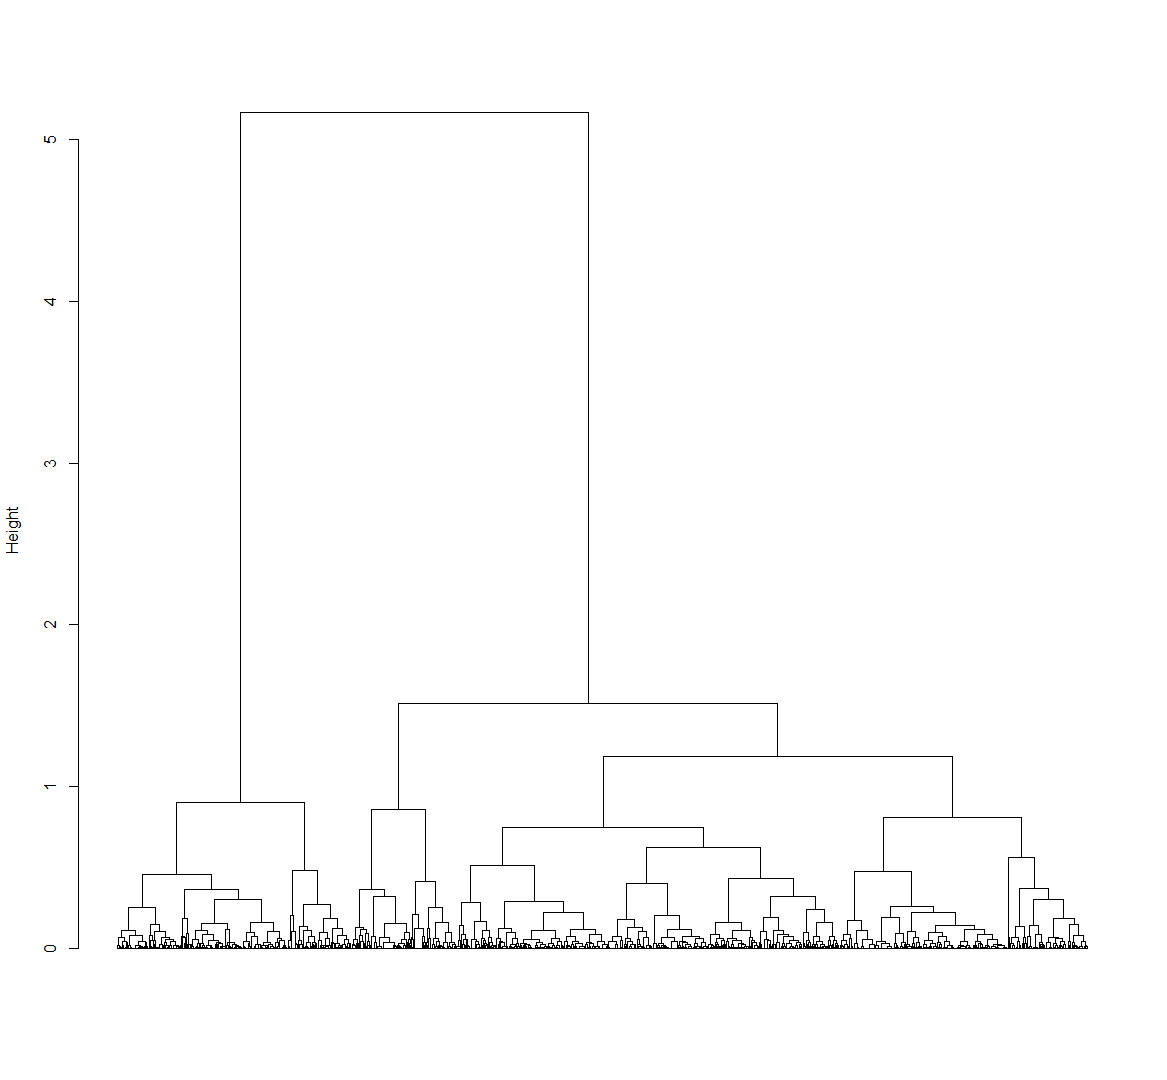
\includegraphics[width=0.8\textwidth]{Images/3_Preprocessing/mimmidend.png}
    \caption{Dendrograma usat pel MIMMI}
    \label{fig:Preprocessing_mimmi_dend}
\end{figure}

En aquest cas, vam escollir k = 4. Amb aquests clústers, realitzats amb les dades que no contenen missing data, es pot imputar la resta de instàncies simplement observant quin és el clúster que els hi pertoca i realitzant la mitja (o la moda, tot i que en aquest cas només s'han imputat variables numèriques).

\subsubsection{MICE} 
\textit{Multivariate Imputation by Chained Equations}, més conegut com MICE, és un altre mètode d'imputació. En aquest, es produeixen múltiples imputacions per variable que es combinen per obtenir el resultat final. Els paràmetres que es van usar per utilitzar-lo en la base de dades van ser: \textit{predictive mean matching} com a mètode (pmm), m (número de imputacions múltiples) 5 i màxim 5 iteracions.

R disposa d'un paquet amb aquest mètode, o sigui que la implementació ja estava feta.

\subsubsection{KNN}

Per imputar les dades usant KNN, s'han utilitzat tan sols les variables numèriques. S'han usat les variables completes (\textit{track\_popularity, album\_popularity, artist\_popularity, artist\_num, energy, loudness, acousticness, liveness, valence, tempo} i \textit{streams}) com a referència.

Per poder imputar, s'han usat com a train les instàncies del dataset amb aquestes variables on el dataset original no contenia missings a la variable a imputar. La "classificació" d'aquest train eren els valors de la variable a imputar (que no tenien missing). Llavors, com a test, s'usen la resta, que són els que contenen missing. D'aquesta manera es poden afegir aquests valors mancants usant el KNN. El valor de k usat ha estat el per defecte, 1, i la distància euclidiana (també el valor per defecte).

Després de les 3 imputacions, la suma total dels valors mancants del dataset era 420. Aquests, però, corresponen a valors mancants en les variables categòriques, especialment en aquelles provinents de APIs ja que va haver-hi alguns problemes. Més endavant s'explicarà com es van sol·lucionar aquests errors.


\subsection{Anàlisi descriptiva post processat}

% Anàlisi, dir quin vam escollir i per què

\subsection{Ampliació de la base de dades mitjançants APIs}

Com ja s'ha mencionat anteriorment, la nostra base de dades originària de \textbf{Kaggle} incloïa diverses variables sobre cançons com ara la seva llargada, timbre, duració, etc. Després d'un primer preprocessament on es van eliminar totes les aparicions de les cançons si l'artista no era el principal, ens vam centrar més en els artistes, ja que l'anàlisi resultava més interessant i prometedor. La falta d'informació detallada sobre els artistes ens va portar a utilitzar diferents APIs per a enriquir el nostre conjunt de dades.

\subsubsection{Selecció d'APIs}

Per a millorar la qualitat i riquesa de les dades, es va decidir incorporar informació addicional sobre els artistes, com ara la seva ubicació \textbf{(País / Ciutat)}, gènere \textbf{(Masculí / Femení / No binari)} i si l'artista és un \textbf{individu} o un \textbf{grup}. A més, també es va incorporar la lletra de les cançons per tal de poder realitzar un \textit{text analysis} més endavant.. Això es va aconseguir mitjançant l'ús de diverses APIs públiques:
\begin{itemize}
    \item \textbf{MusicBrainz API}: Per obtenir detalls específics dels artistes, incloent si són solistes o grups, i el gènere del grup basat en els seus membres.
    \item \textbf{CountriesNow API}: Per verificar si una ciutat determinada es troba dins d'un país específic, evitant així inconsistències en la ubicació.
    \item \textbf{RestCountries API}: Per obtenir la capital d'un país quan la ciutat de l'artista no està disponible o no es pot verificar correctament.
    \item \textbf{Genius API}: Per obtenir els lyrics de les cançons. S'ha usat amb la llibreria de \textit{Python} \textit{lyricsgenius} .
\end{itemize}

\subsubsection{Gestió d'errors i tècniques de millora}

Per a assegurar la fiabilitat i precisió de les dades recopilades, es van implementar diverses estratègies:
\begin{itemize}
    \item Esperar un temps prudencial entre trucades a la API per evitar sobrecàrregues i possibles bloquejos.
    \item Realitzar múltiples intents per cada trucada a l'API, gestionant els errors temporals de manera eficient.
    \item Substituir els valors no disponibles (\textit{NA}) per les capitals dels països corresponents quan la informació de la ciutat de l'artista no es trobava o era incorrecta.
    \item Verificació manual per a casos on les dades automàticament recollides no eren coherents, com ara ciutats que no pertanyien al país indicat o països erròniament identificats com a ciutats.
\end{itemize}

Malgrat l'aplicació d'aquestes mesures, alguns errors en la localització d'artistes van requerir correccions manuals, especialment en casos on les ciutats no concordaven amb els països o quan la informació retornada per les APIs era incorrecta a causa de la confusió amb altres artistes de nom similar. Aquestes situacions van ser poc freqüents però destacables, ja que reflecteixen les limitacions inherents a l'ús de dades automàticament recollides i la importància de la revisió humana en la curació de conjunts de dades.

\subsubsection{Resultats}

Després de l'execució de l'script i la implementació de les tècniques esmentades, es va obtenir un conjunt de dades considerablement millorat, amb informació més completa i precisa sobre els artistes i amb les lletres de les cançons. Aquest enriquiment de les dades obre noves possibilitats per a l'anàlisi, permetent estudis més detallats i específics sobre la música i els seus creadors en la plataforma Spotify.







\newpage

\section{Clústering avançat} 

En aquesta secció s'exploraran diferents tècniques avançades de clustering alhora que s'analitzaran i es compararan els resultats obtinguts. Cal mencionar en tots que els objectius de la creació de classes pot resultar diferent sobretot segons el mètode utilitza ja que, per exemple, en el \textit{K-modes} tan sols volem formar clústers per variables categòriques o en el \textit{time series clustering} volem agrupar instàncies de cançons segons una sola variable al llarg del temps.

\subsection{Clústering jeràrquic} \label{section:clustering_jerarquic3}

El clustering jeràrquic és un mètode d'agrupament de dades que no requereix donar-li el nombre de grups com a paràmetre, ja que es representa amb dendrograma (que mostra la relació de similitud entre els elements) i a partir d'allà es pot escollir la k. Aquest mètode ja es va explorar el quatrimetre passat.

En aquest apartat es fa un clústering jeràrquic però afegint les noves variables creades durant el preprocessament de les dades per veure de quina manera aquestes variables afecten a aquest agrupament. A l'agrupament les variables que no han estat incluides han estat week\_index i day\_release ja que s'ha considerat que es feient millor els clústers sense afegir-les. Tampoc s'han incluit les variables track\_id, track\_name, album\_name i artist\_name. 

% Foto del dendrograma sense pintar
\begin{figure}[H]
    \centering
    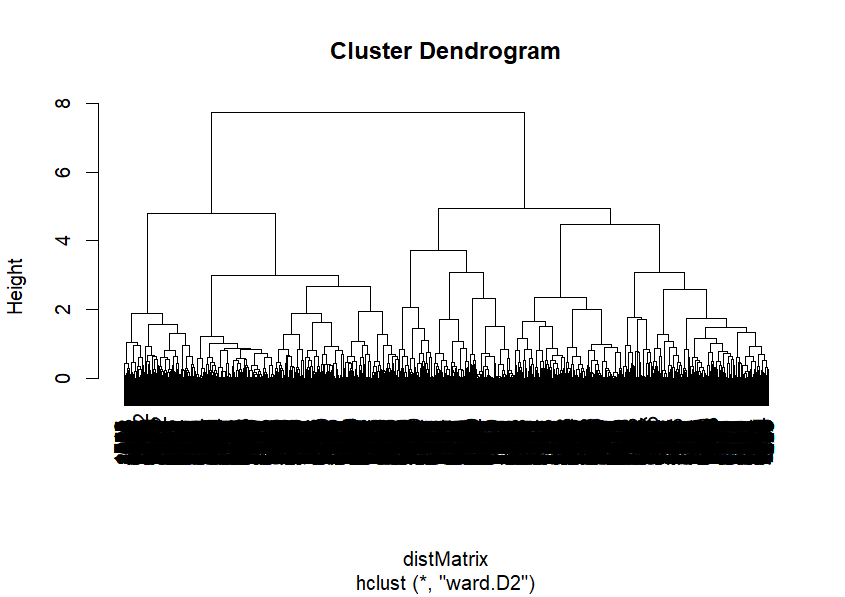
\includegraphics[width=0.8\textwidth]{Images/4_clustering/herarchical/dendogram.png}
    \caption{Dendrograma del clustering jeràrquic}
    \label{fig:dendogram}
\end{figure}

Observant el dendrograma, podem veure que es podria dividir entre dues classes, però per fer el profiling considerem que és millor agafar més classes. L'han passat vam triar 4 clústers, però en el cas d'ara ens quedarien les classes poc balancejades. Per això, triem 5 clústers.  

Amb el dendrograma resultant, es divideixen els 5 clústers de la següent manera: 

\begin{figure}[H]
    \centering
    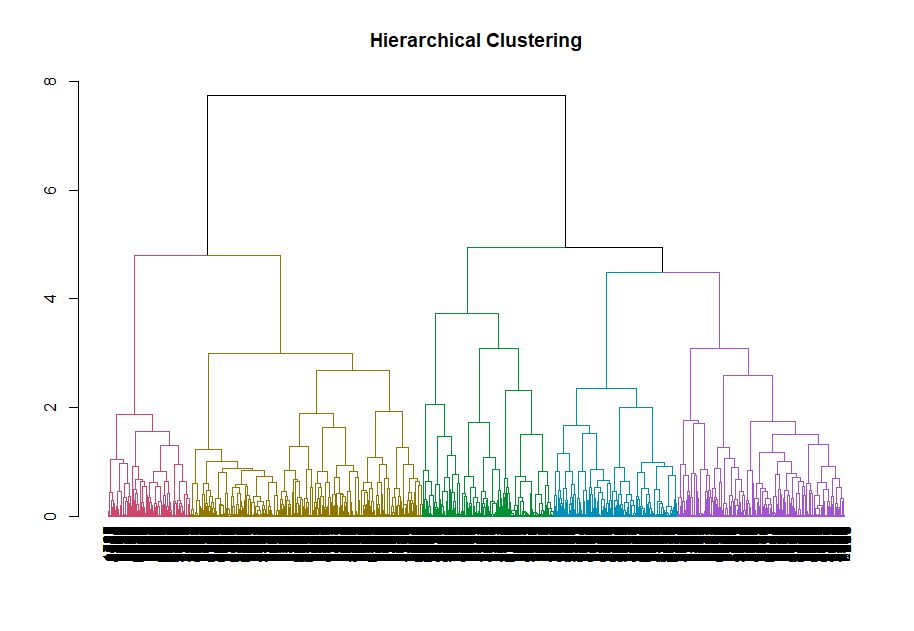
\includegraphics[width=0.8\textwidth]{Images/4_clustering/herarchical/hierarchical_dendogram_colors2.png}
    \caption{Dendrograma del clustering jeràrquic després de crear els clústers}
    \label{fig:hierarchical_dendogram_colors2}
\end{figure}

Abans de realitzar el profiling del clústering jeràrquic, s'ha realitzat un PCA per poder observar els clusters que s'han identificat en el clústering jeràrquic en les dos primeres components principals.

\begin{figure}[H]
    \centering
    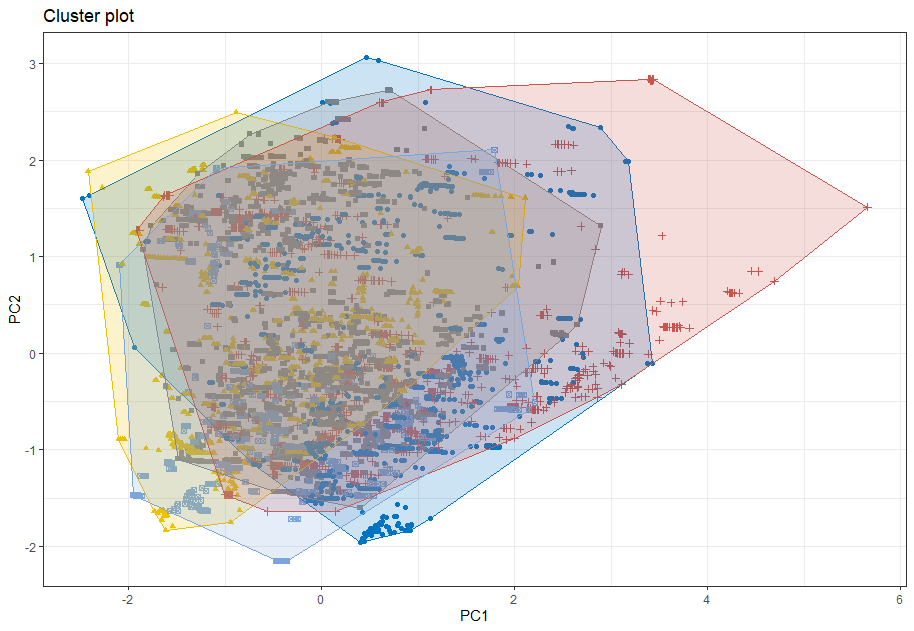
\includegraphics[width=0.7\textwidth]{Images/4_clustering/herarchical/pca_hierarchical.png}
    \caption{Resultats del clústering jerarquic}
    \label{fig:pca_hierarchical}
\end{figure}

Com es pot observar, tenim 5 clústers, uns semblen més dispersos i altres més densos indicant variacions en la cohesió interna dels grups. Tot i així, és important recalcar que les dos primeres components no capturen una gran informació de les dades (17\% el primer component i 14\% el segon).

Encara que no es pot observar una clara divisió dels clústers degut al baix percentatge de variància explicada en les dos primeres components, amb  el profiling que s'ha realitzat posteriorment, s'examinarà les dades en la seva totalitat i les característiques de cada clúster.   

La mida dels clústers finals és de:
\begin{table}[H]
\centering
\begin{tabular}{|c|c|c|c|c|}
\hline
1    & 2    & 3   & 4   & 5 \\ \hline
1574 & 1997 & 2785 & 1489  & 990  \\ \hline
\end{tabular}
\caption{Resultat del clústering jerarquic}
\label{tab:clustering_results}
\end{table}

Es pot veure que l'últim clúster té una mida més petita que la resta, tot i així, la mida de tots els clústers és bastant similar.

\subsection{K-modes}

El K-modes és un algoritme de clustering i és una extensió del k-means, un algoritme que ja hem treballat en aquesta assignatura. L'algorisme fa bàsicament el mateix però en comptes d'utilitzar dades numèriques, utilitza exclusivament dades categòriques. En el nostre cas hem seleccionat totes les variables categòriques que ja teniem ("pop","hip\_hop", "collab","rank\_group"...) i a més les noves variables afegides durant el preprocessament ("gender", "is\_group", "nationality",\"city"). La variable lyrics no s'ha inclòs en el clustering.

Divideix les dades en un nombre k de grups basant-se en la similitud entre ells. La k, com al k-means, és un hiperparàmetre que hem de triar nosaltres. Per veure la similitud de les dades, en comptes d'utilitzar la distància euclidiana, utilitzem una mesura de disimilitud per a dades categòriques.

Utilitzant el paquet klaR en R, hem fet servir kmodes() donant-li el hiperparàmetre k = 4. Com no es poden utilitzar mètriques de validació per les variables categòriques, s'ha triat la k no agafant un nombre molt gran, i a partir del clustering jeràrquic que vam fer l'any passat. 

Un cop s'ha realitzat el K-Modes, s'ha realitzat un Anàlisi dels Components Principals (ACP) per visualitzar la distribució dels clústers respecte les variables numèriques. No s'ha observat una classificació clara de les variables numèriques en els clústers realitzats amb les variables categòriques. Tot i així, en la cinquena i sisena dimensió (8,5\% i 6\% de variància explicada respectivament) si que s'observa una petita separació entre clústers.  \\

\begin{figure}[H]
    \centering
    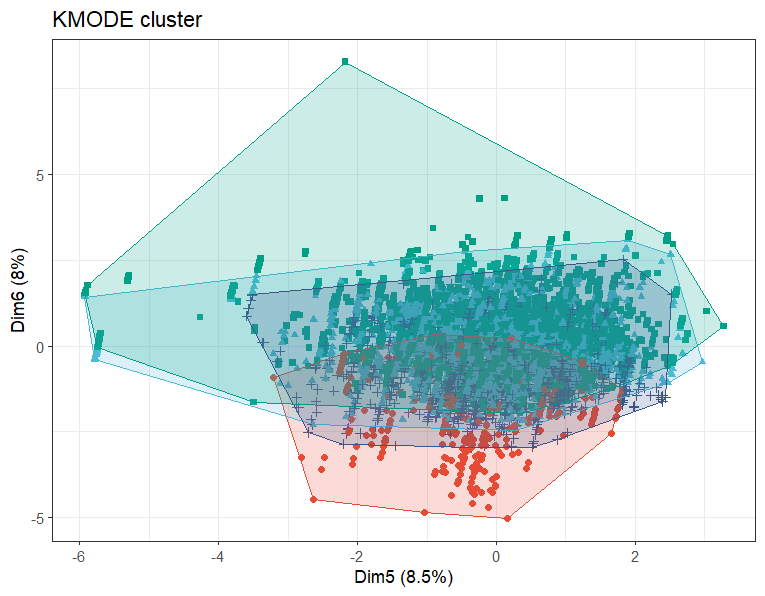
\includegraphics[width=0.7\textwidth]{Images/4_clustering/KMODES/kmodes1.png}
    \caption{Resultats del K-Modes en la 5ª i 6ª dimensió}
    \label{fig:kmodes1}
\end{figure}

La dimensió 5 està relacionada amb l'speechines i el tempo d'una cançó i la dimensió 6 està més relacionada amb el número d'artistes, la duració i la danceability d'una cançó. Per tant, es podria indicar que el K-Means divideix els clústers segons aquestes característiques. Tot i així, cal recalcar que aquestes dimensions només expliquen un 16\% de la variància total de les dades, per tant, caldria fer el profiling per poder afirmar aquesta conclusió.

\begin{figure}[H]
    \centering
    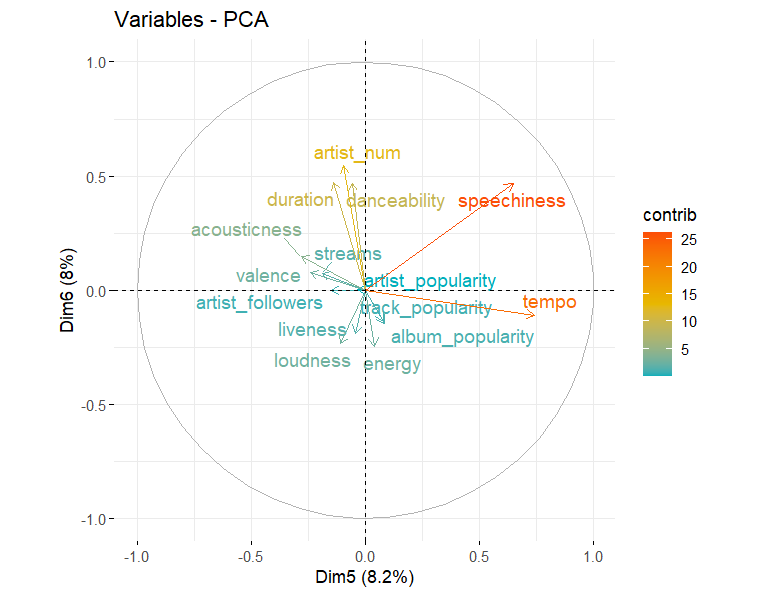
\includegraphics[width=0.7\textwidth]{Images/4_clustering/KMODES/kmodes2.png}
    \caption{Variables i la seva contribució en el 5é i 6é components principals}
    \label{fig:kmodes2}
\end{figure}

Un cop fet ja s'ha experimentat amb el k-means i amb el k-modas, s'ha trobat interessant  fer ús del k-prototypes. Aquesta és una tècnica que barreja les variables numèriques i categòriques. S'ha utilitzat la funció kproto() de clustMixType per fer el clustering. Com amb el k-means, basant-nos en els resultats de l'últim agrupament, s'ha utilitzat el número de clústers k=4. També s'han afegit més paràmetres. El paràmetre lambda s'encarrega d'equilibrar la importància entre els dos tipus de variales, també hem posat un màxim d'iteracions i el nombre d'ejecucions a fer amb diferents centroides inicials (nstart). 

\subsection{CURE}
Clustering Using REpresentatives (\ref{guha_1998_cure}) és una tècnica avançada de clústering centrada en millorar el rendiment d’aquest tipus d’algorismes per bases de dades especialment grans. Es basa en el concepte de trobar uns punts representatius inicials i realitzar el clústering amb aquests. Un cop es troben uns centroides adequats, es calculen les distàncies de la resta dels punts a aquests i s’escull el millor.

S’ha escollit realitzar-lo usant tant les variables numèriques com algunes categòriques (gèneres...). Per tal de poder combinar aquestes variables mixtes, les categòriques s’han transformat prèviament en one-hot-encoding. A més, per evitar problemes amb les magnituds (algunes numèriques tenien valors entre 0 i 1 mentres que d’altres arribaven als milions), les variables numèriques s’han escalat usant la funció scale de R.

\begin{figure}[H]
    \centering
    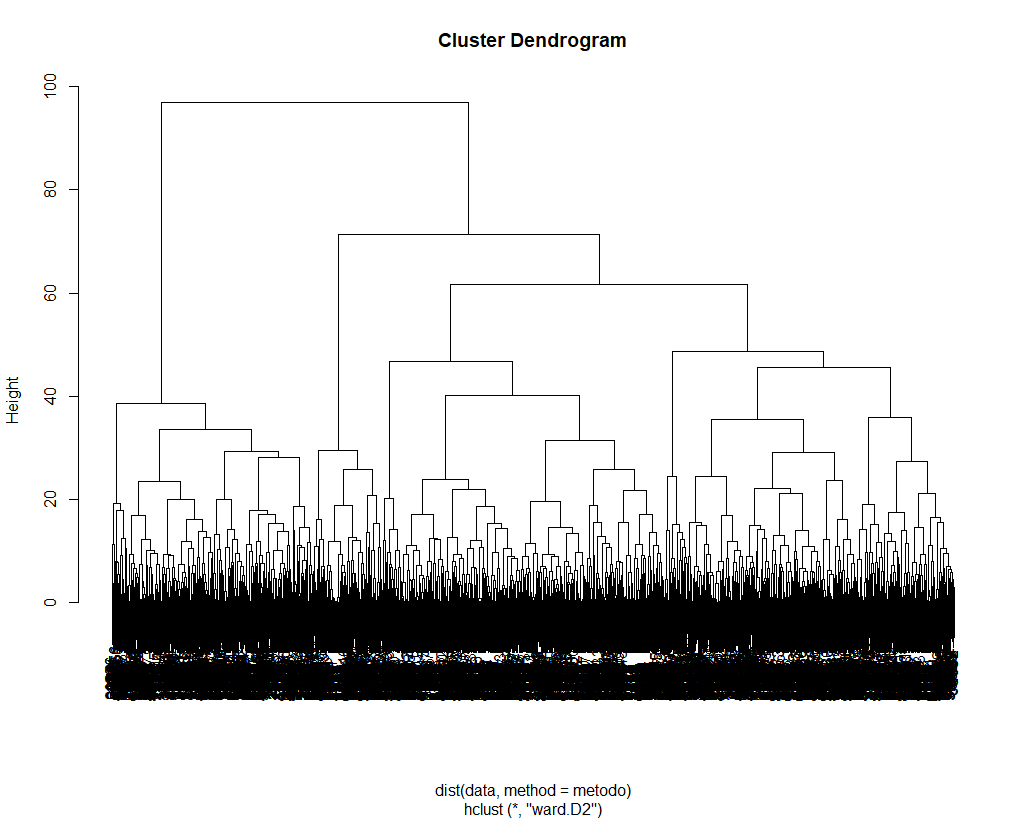
\includegraphics[width=0.8\textwidth]{Images/4_clustering/CURE/curedendrogram.png}
    \caption{Dendrograma de les dades usades pel CURE (jeràrquic, amb ward D2)}
    \label{fig:CURE_dend}
\end{figure}

La distància usada ha estat la euclidiana, ja que després d’aquest petit processat de les dades es podia utilitzar. Amb un  clústering jeràrquic inicial s’ha observat que un bon punt de tall era 4 observant la figura \ref{fig:CURE_dend}, i per tant s’ha escollit aquesta k. La r escollida, és a dir, el percentatge de representatius, ha estat 0.25.

Els 4 clústers dels representatius han quedat amb el següent nombre de cançons en cada un (taula \ref{tab:CURE_taularep}):

\begin{table}[H]
\centering
\begin{tabular}{lllll}
\cline{1-4}
\multicolumn{1}{|c|}{1}   & \multicolumn{1}{c|}{2}   & \multicolumn{1}{c|}{3}    & \multicolumn{1}{c|}{4}   &  \\ \cline{1-4}
\multicolumn{1}{|c|}{653} & \multicolumn{1}{c|}{654} & \multicolumn{1}{c|}{1211} & \multicolumn{1}{c|}{133} &  \\ \cline{1-4}
                          &                          &                           &                          &  \\
                          &                          &                           &                          & 
\end{tabular}
\caption{Resultat del clústering dels representatius}
\label{tab:CURE_taularep}
\end{table}

A partir d’aquests, es poden assignar clústers a la resta de dades. El resultat es pot observar a \ref{tab:CURE_taulanorep}.

\begin{table}[H]
\centering
\begin{tabular}{lllll}
\cline{1-4}
\multicolumn{1}{|c|}{1}    & \multicolumn{1}{c|}{2}    & \multicolumn{1}{c|}{3}   & \multicolumn{1}{c|}{4}   &  \\ \cline{1-4}
\multicolumn{1}{|c|}{3266} & \multicolumn{1}{c|}{1939} & \multicolumn{1}{c|}{670} & \multicolumn{1}{c|}{309} &  \\ \cline{1-4}
                           &                           &                          &                          &  \\
                           &                           &                          &                          & 
\end{tabular}
\caption{Resultat del clústering dels no representatius}
\label{tab:CURE_taulanorep}
\end{table}

Observem com han quedat lleugerament desbalancejats. Se’ns presenta un grup 1 amb moltes de les instàncies, seguit d'un grup 2 que també en té moltes. D'altra banda, els clústers 3 i 4 tenen pocs elements (tot i que el 3 té molts representatius). Els resultats d'aquest clústering es poden visualitzar usant les dues primeres dimensions del PCA, com es pot observar a la figura \ref{fig:CURE_res}.

\begin{figure}[H]
    \centering
    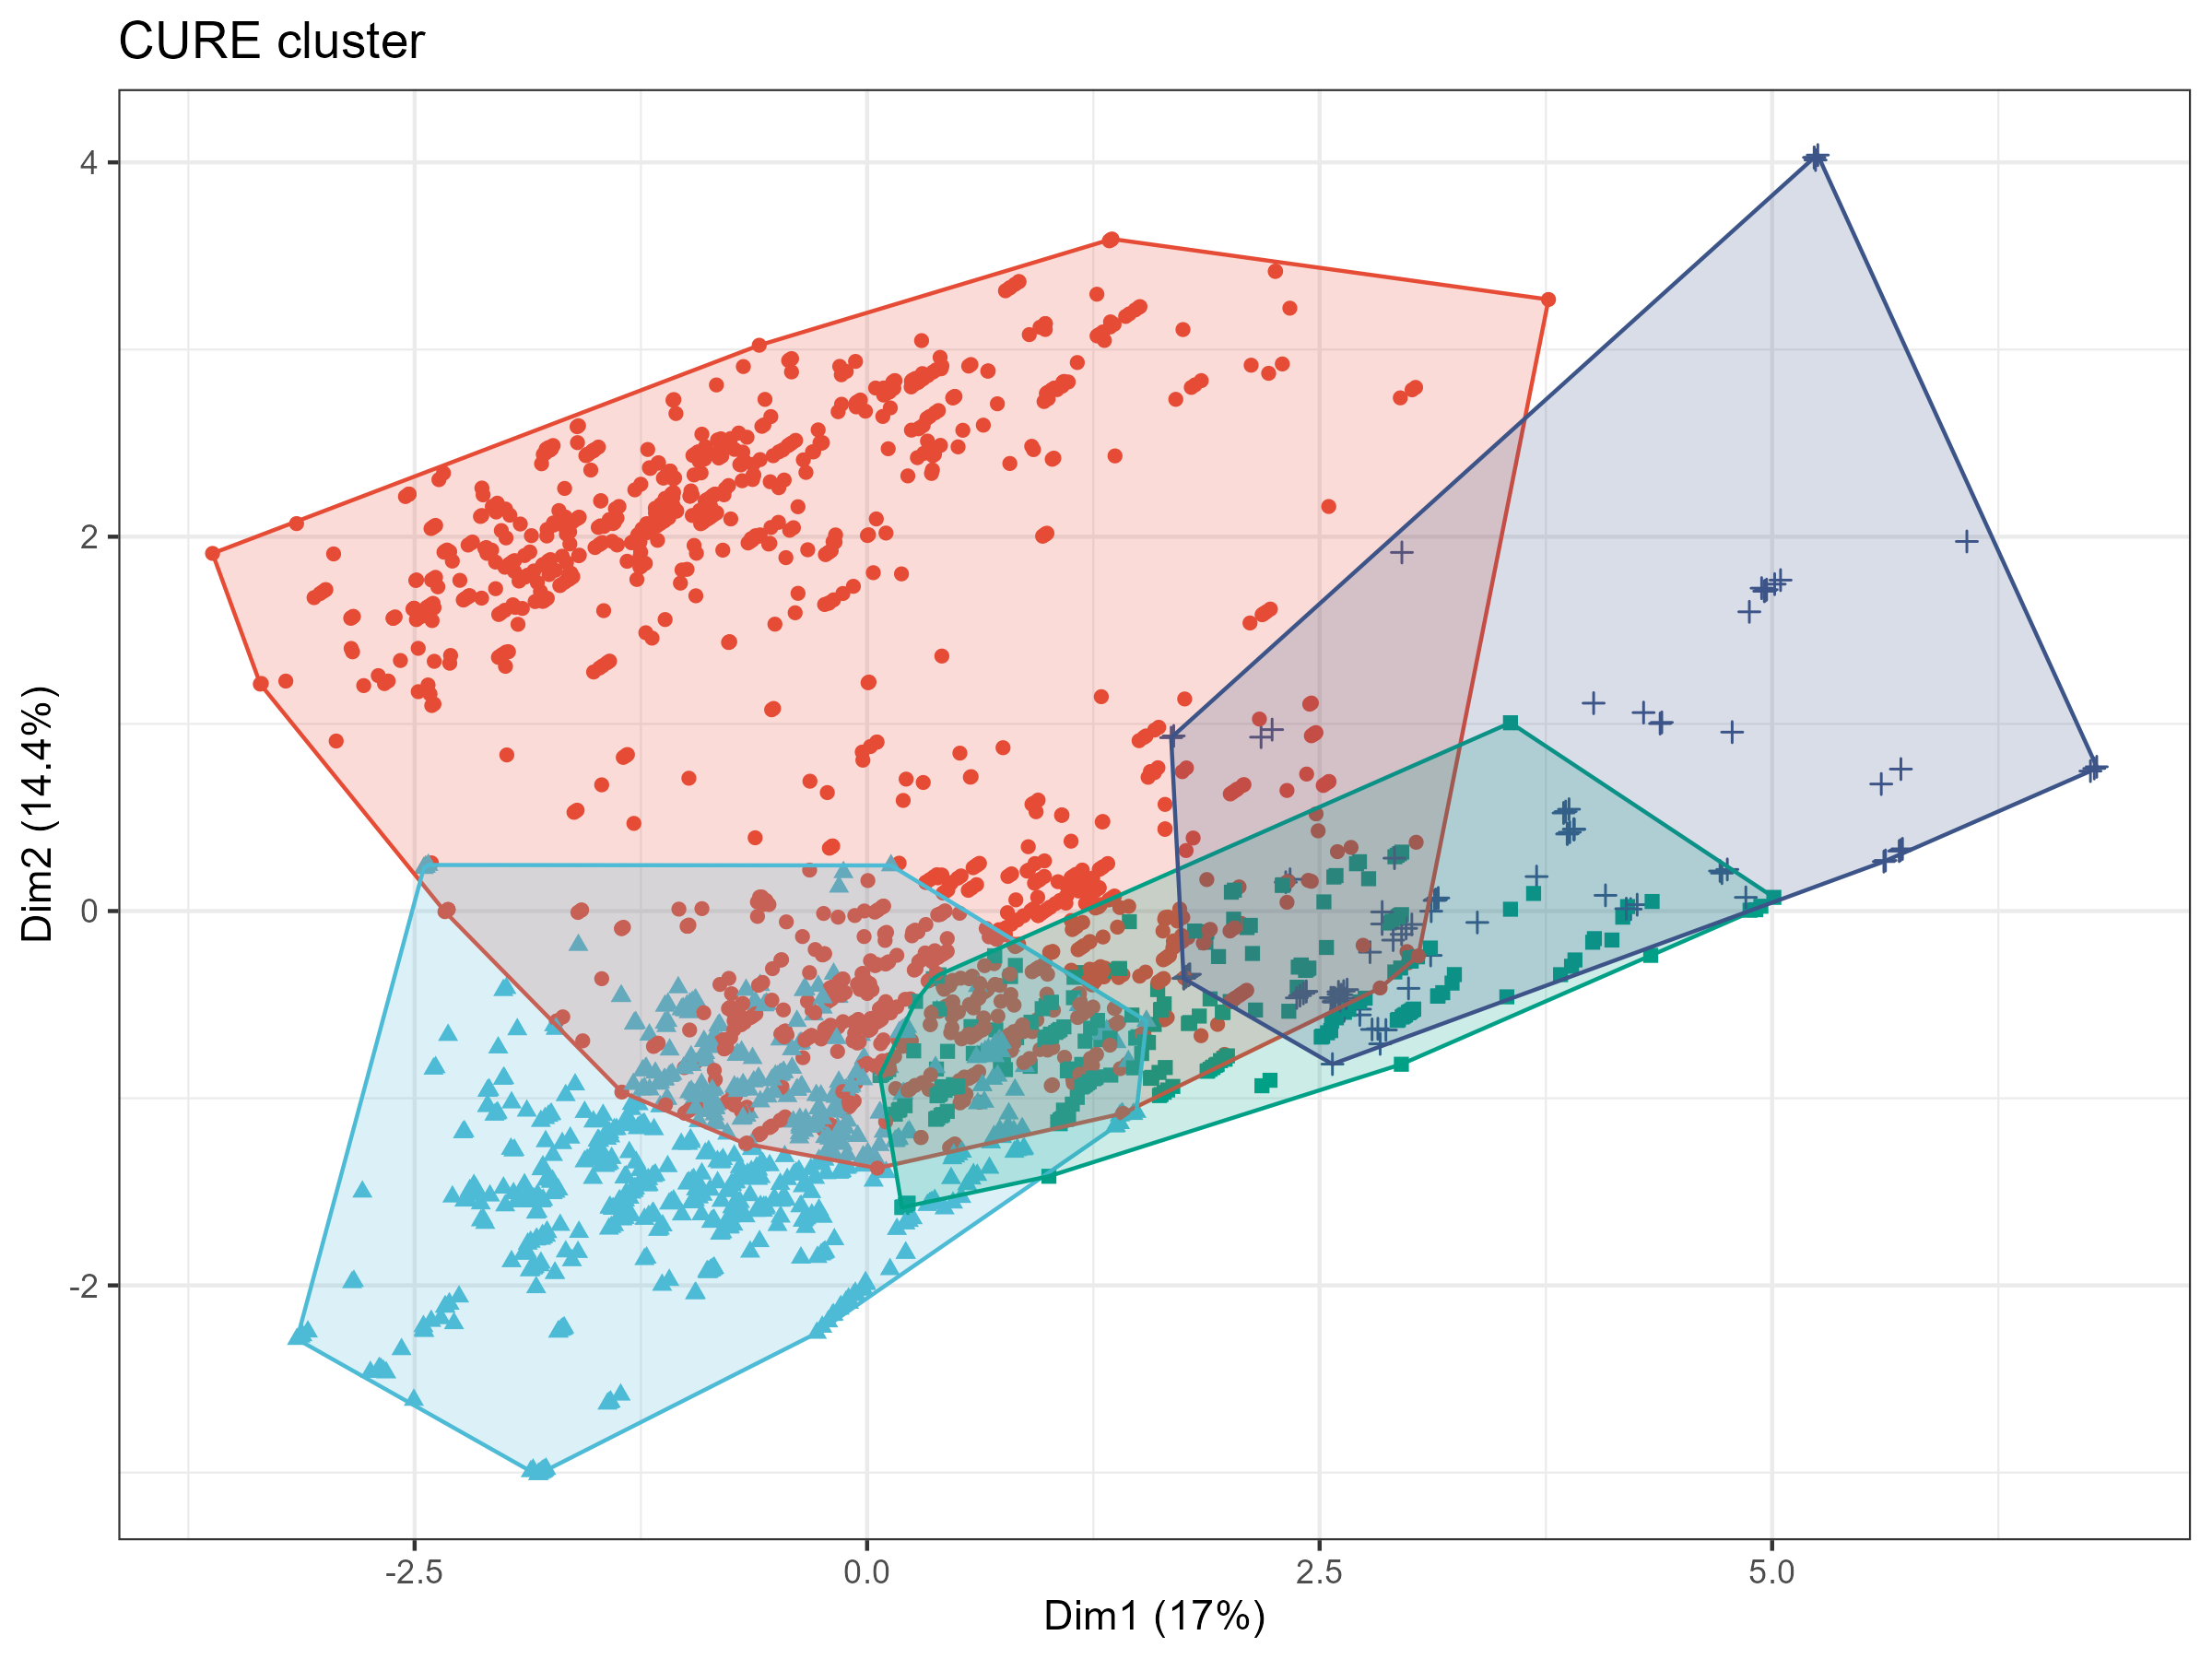
\includegraphics[width=0.8\textwidth]{Images/4_clustering/CURE/cure.png}
    \caption{Resultats del clústering usant CURE (4,0.15)}
    \label{fig:CURE_res}
\end{figure}

S'observa un gran clúster vermell, corresponent probablement al clúster 1. Aquest ocupa un núvol de punts situat a l'espai superior, així com la part central del núvol inferior. Amb valors negatius tant de la primera com de la segona dimensió trobem el clúster blau clar, corresponent al número 2, que és el segon més gran. Finalment, el clúster verd es situa al centre del núvol inferior, amb valors de la dimensió 2 bastant baixos, i el clúster 4, de color blau fosc, és el que engloba els punts amb valors més alts de la dimensió 1.

\subsection{DBSCAN}

El DBSCAN (\cite{dbscan}) és una tècnica de clústering basada en densitat. Per tal de poder observar millor com es reparteixen les nostres dades en aquest aspecte, el primer pas realitzat ha sigut un anàlisi dels components principals (PCA) (figura \ref{fig:DBSCAN_pca}). Aquest, a diferència de l'any passat, no ha estat realitzat en profunditat: tan sols ha estat usat com a tècnica de visualització de dades.

\begin{figure}[H]
    \centering
    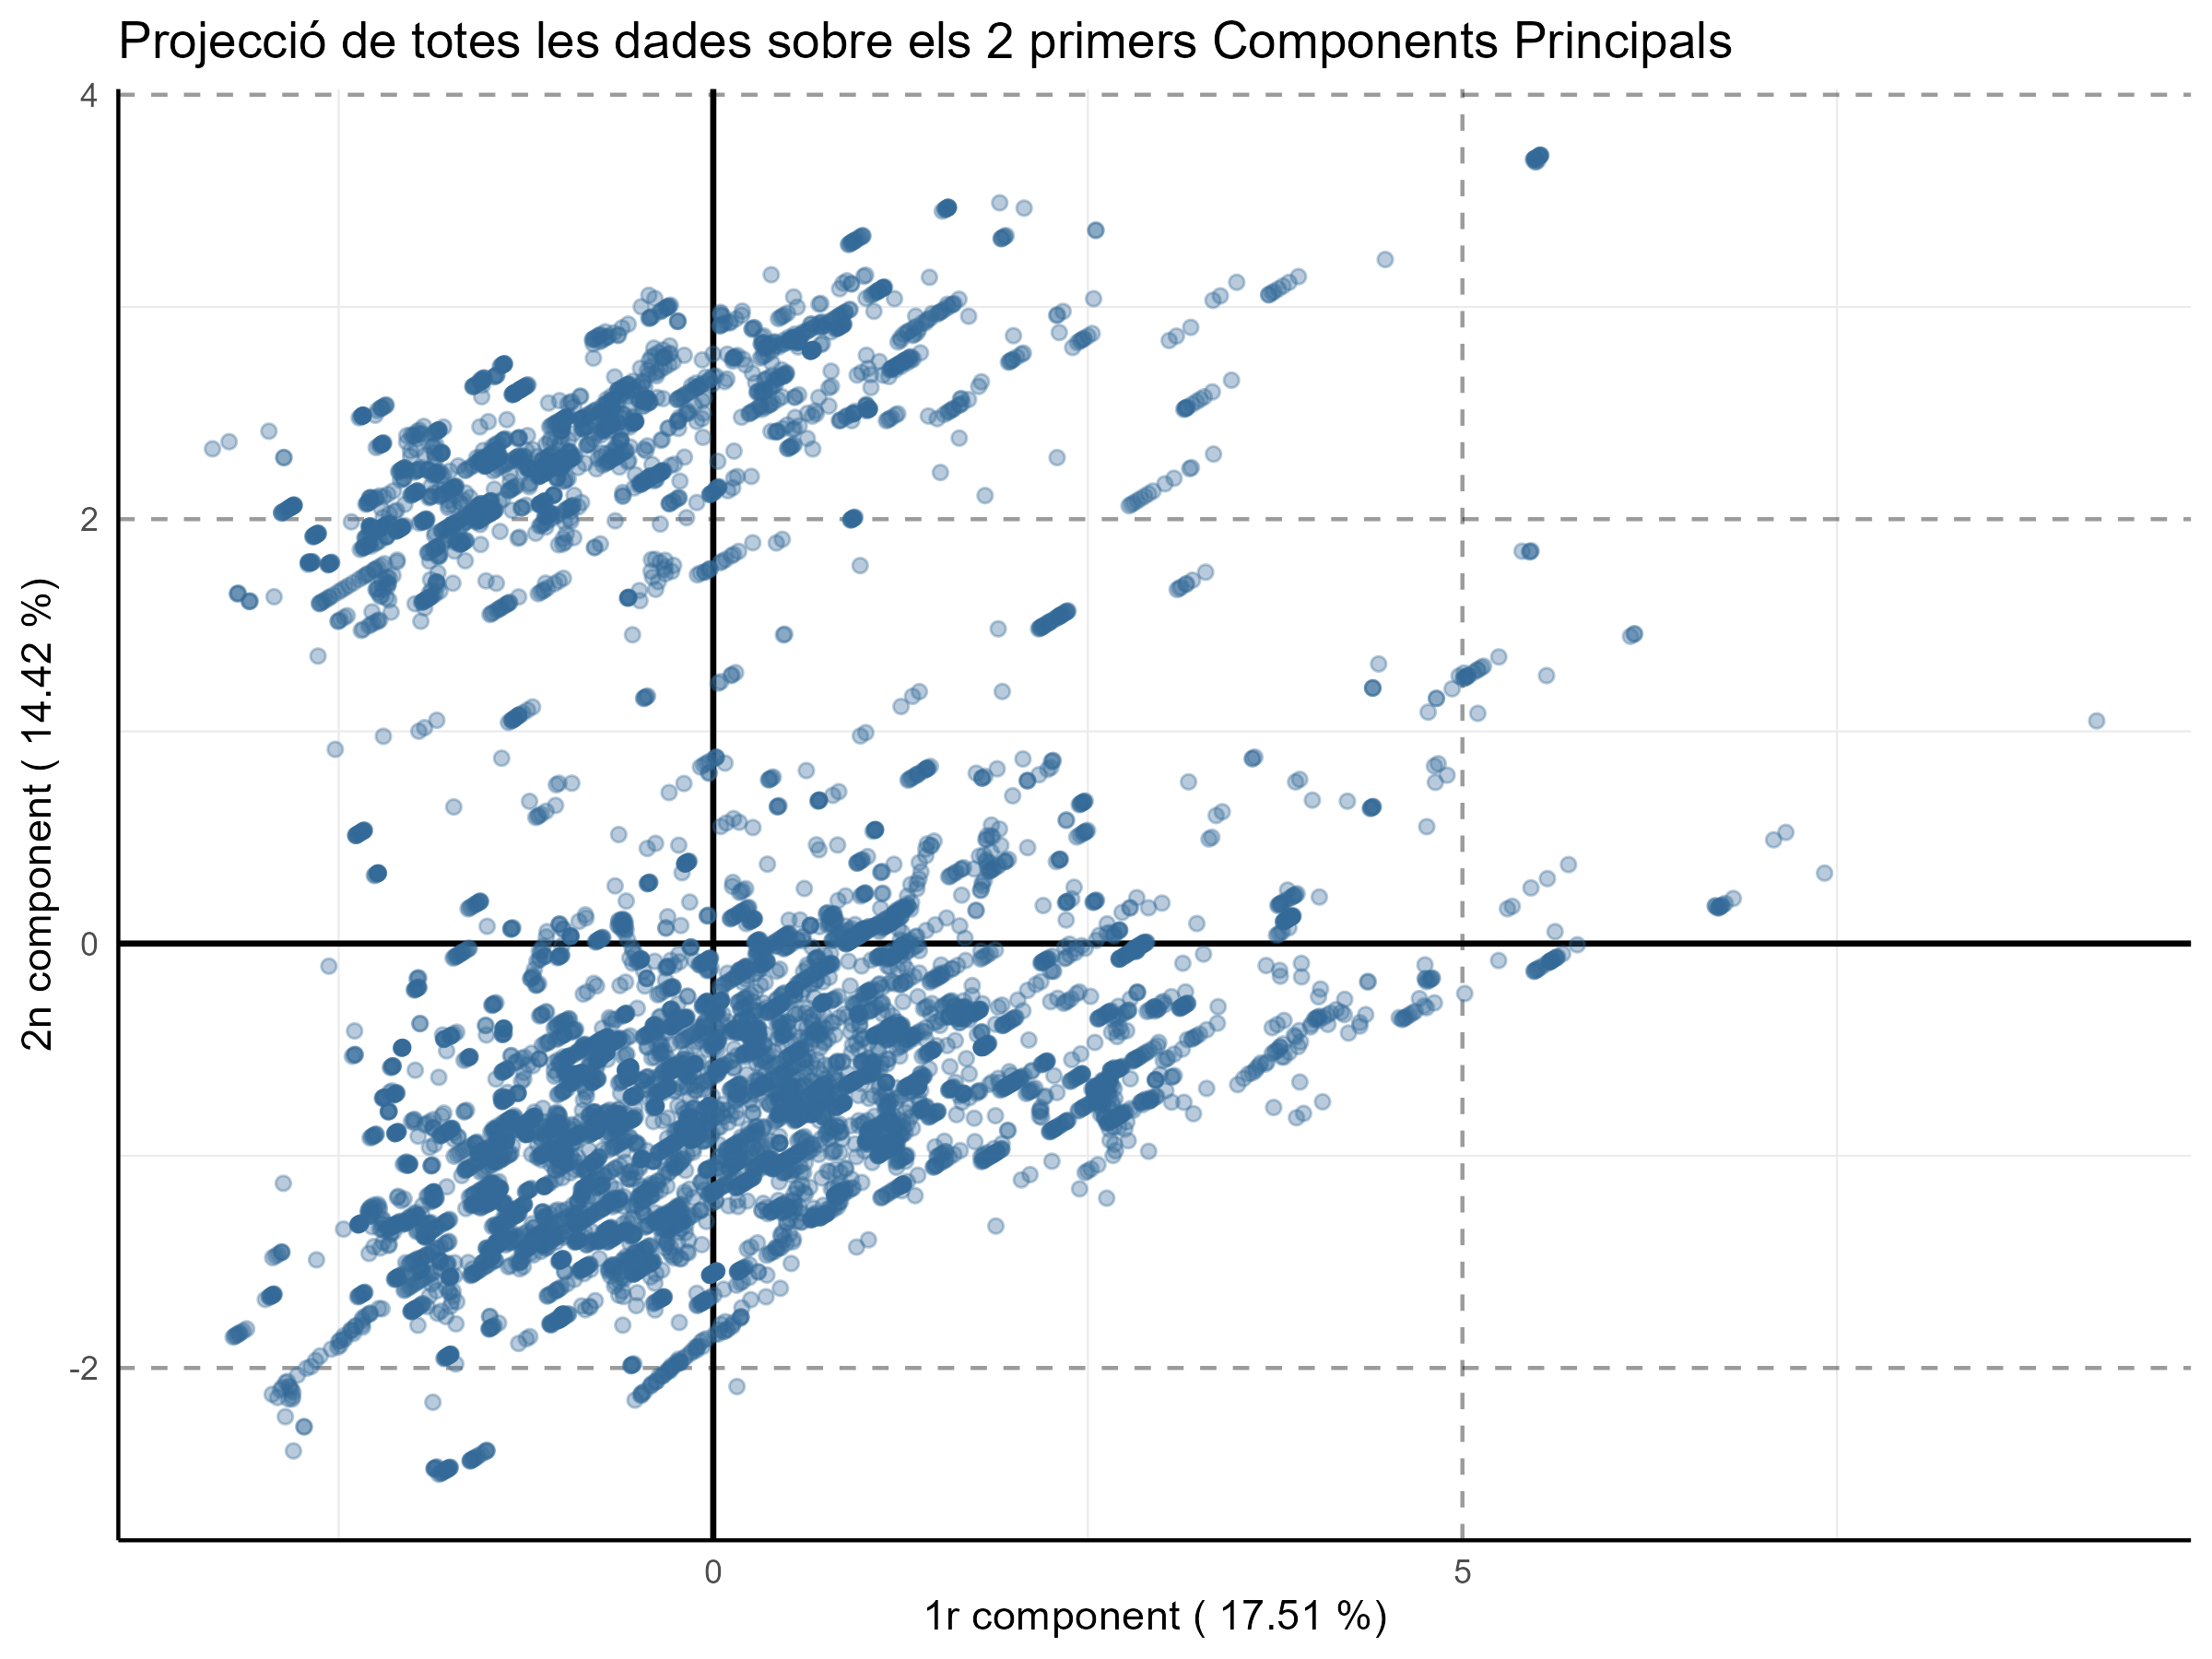
\includegraphics[width=0.8\textwidth]{Images/4_clustering/DBSCAN/dbscanpca.png}
    \caption{Dades descomposades en els dos primers components principals}
    \label{fig:DBSCAN_pca}
\end{figure}

A simple vista, basant-nos en les dues components principals, observem dos grans grups: un amb valors negatius de la segona component i un altre amb valors positius. Analitzant les variables que influeixen en aquests components (figura \ref{fig:DBSCAN_pca_contrib}), sembla ser que el grup inferior conté cançons més populars, mentres que l'altre conté cançons més antigues i per tant menys populars (Dimensió 2). La dimensió 1 ens indica com d'acústica o trista és la cançó: valors negatius indiquen cançó positiva, amb energia i forta (potent) mentre que valors positius indiquen una major \textit{acousticness}.

\begin{figure}[H]
    \centering
    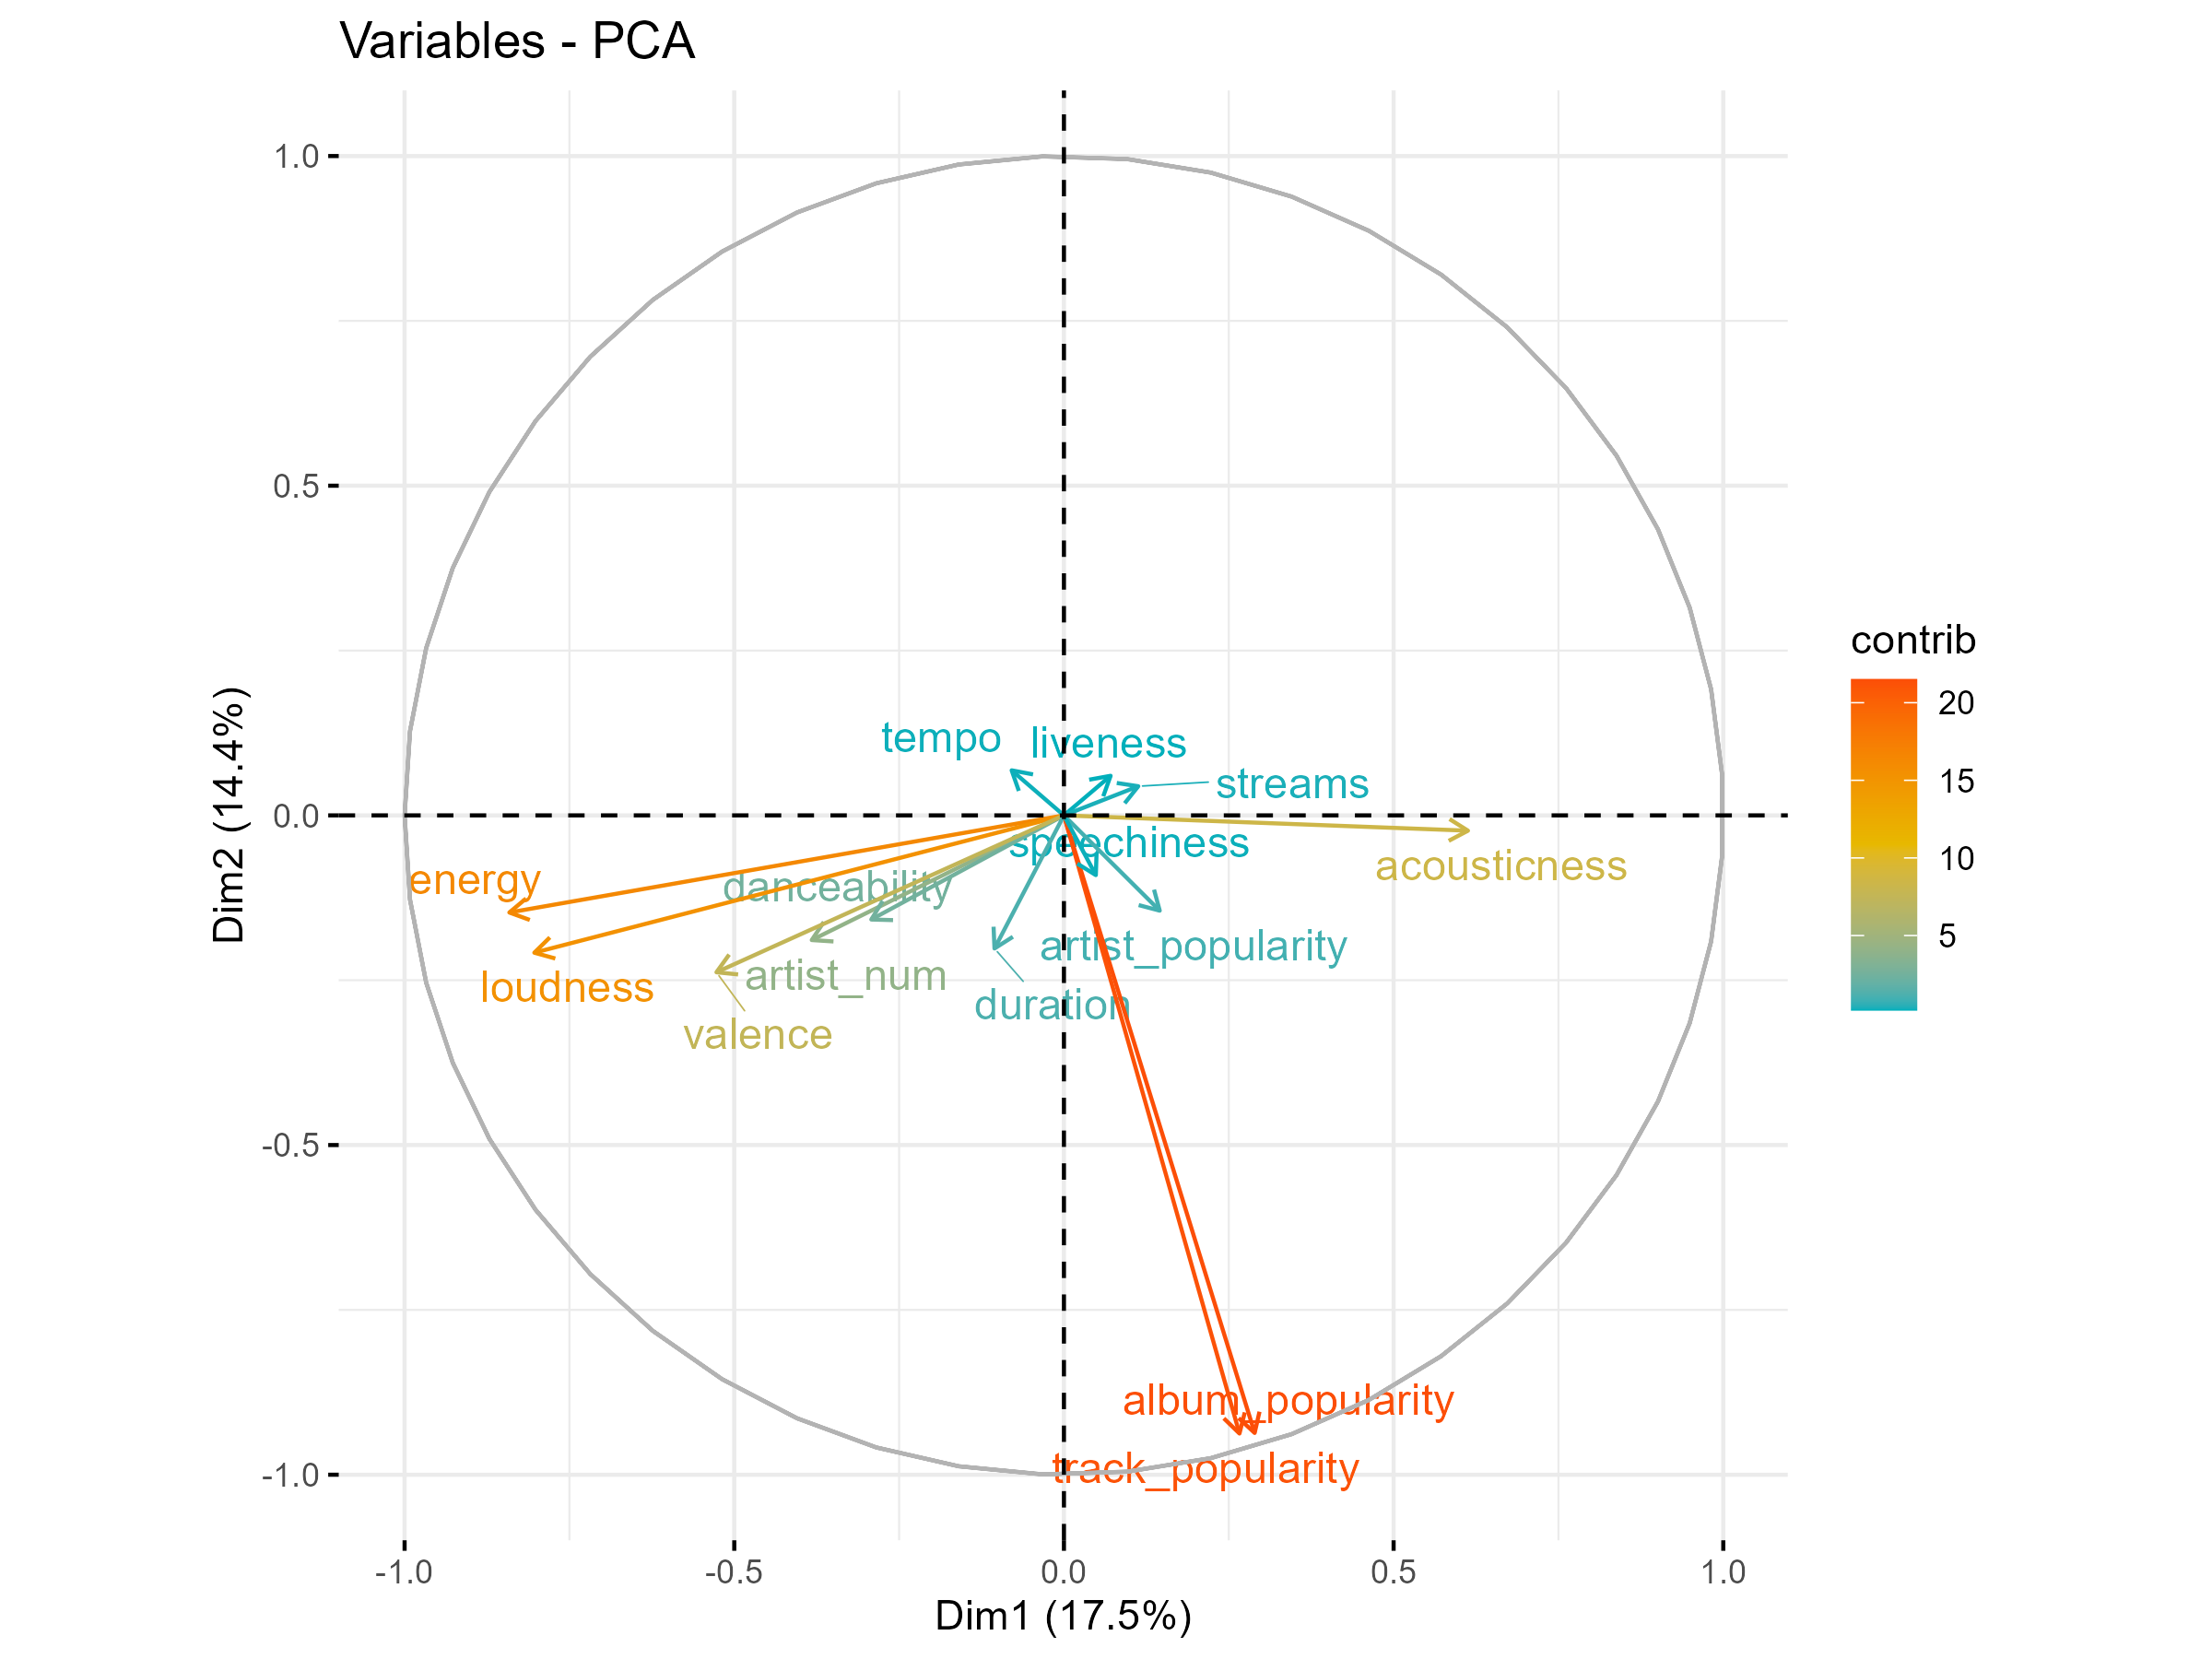
\includegraphics[width=0.8\textwidth]{Images/4_clustering/DBSCAN/dbscanpcacomponents.png}
    \caption{Variables i la seva contribució en cada un dels dos primers components principals.}
    \label{fig:DBSCAN_pca_contrib}
\end{figure}

Abans de realitzar el DBSCAN, el clústering basat en densitat, s’ha creat un petit k-means per tal d’observar la nostra distribució de dades  (figura \ref{fig:KMEANS}). En aquest cas, s’ha usat una k amb valor 5. Cal destacar que a partir d'aquest moment, usarem unes dades normalitzades ja que les distàncies (concretament, els rangs de valors de les variables) poden afectar a aquests clústers.

\begin{figure}[H]
    \centering
    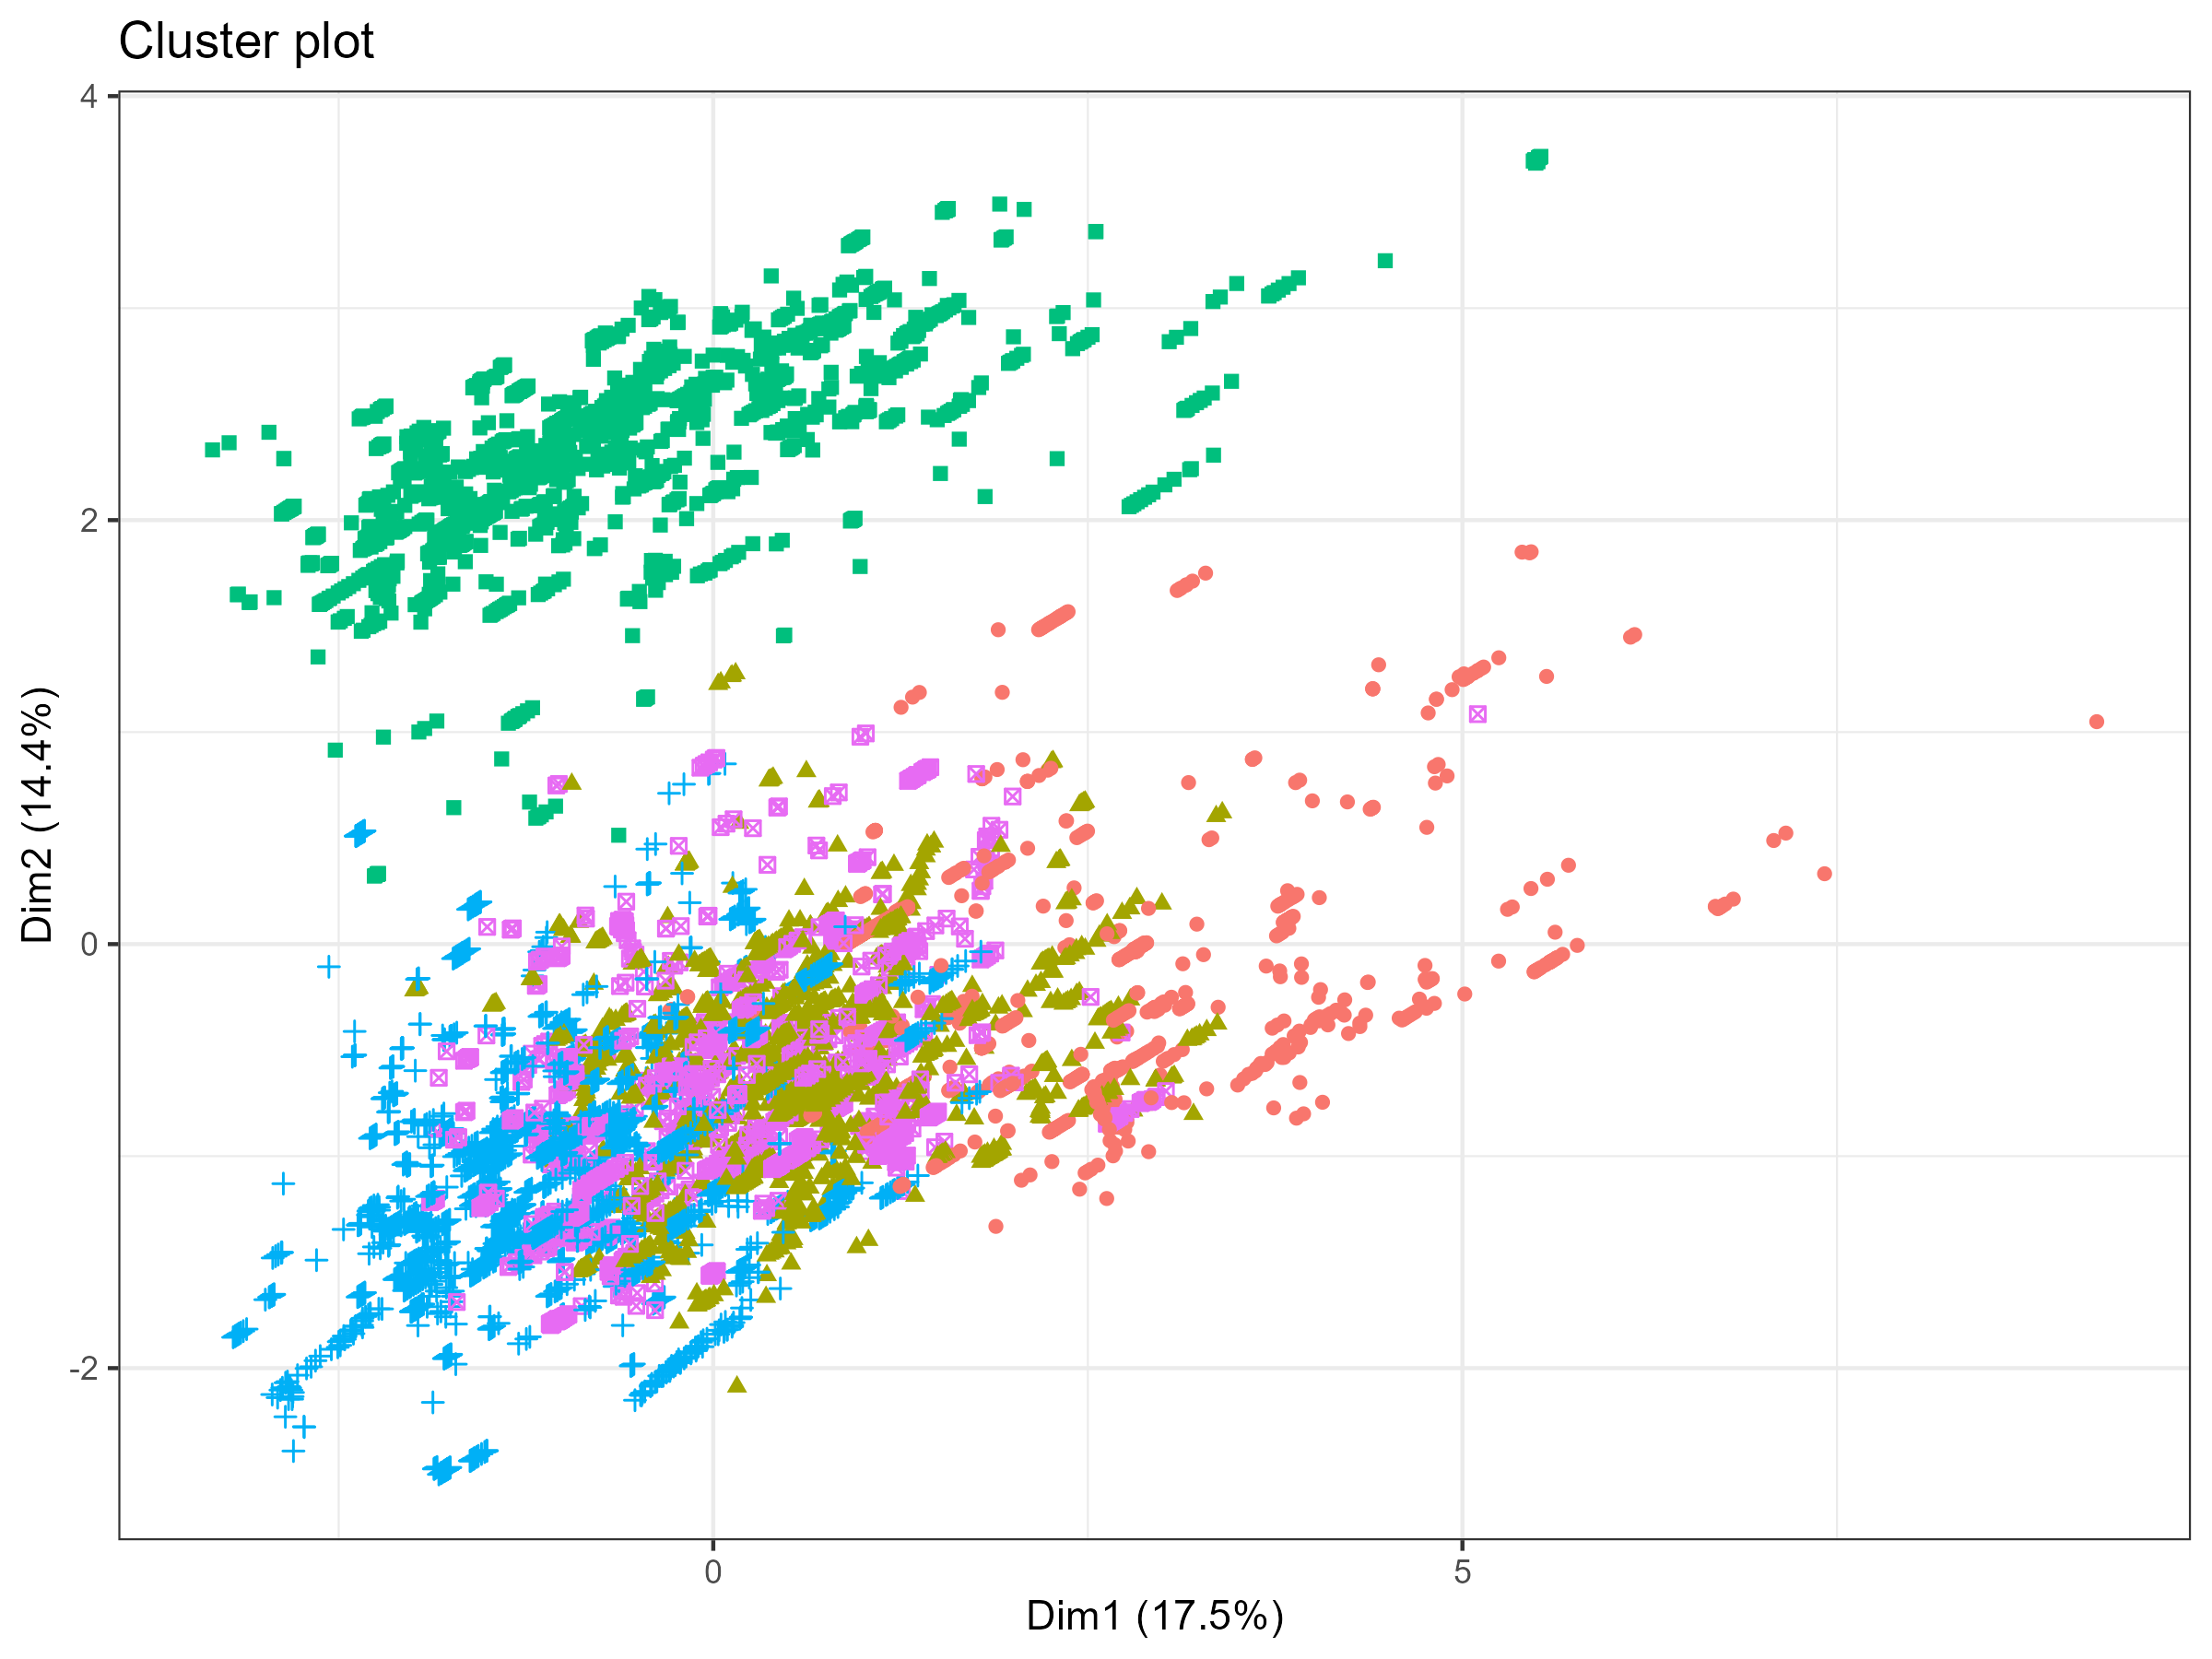
\includegraphics[width=0.8\textwidth]{Images/4_clustering/DBSCAN/kmeans.png}
    \caption{Resultats del clústering usant K-MEANS.}
    \label{fig:KMEANS}
\end{figure}

El grup superior, vist anteriorment, ha estat catalogat pràcticament de manera íntegra en el clúster verd. Pel que fa l’altre, s’ha repartit en funció de la dimensió 1: valors més baixos corresponen al clúster blau, els mitjanament baixos al violeta, els mitjanament alts a un verd més marronós i els alts a un taronja. Els dos clústers amb valors mitjos, el violeta i el marró, han quedat bastant barrejats. En general, però, els clústers creats són bastant bons, i ens serviran de referència per comparar amb els trobats pel DBSCAN.

Observant aquests mateixos clústers en la tercera i quarta dimensió (figura \ref{fig:KMEANS_34}), les dades queden molt més barrejades . Els clústers verds, taronja i marró queden completament inseparables, i els únics que podriem distingir serien el blau, amb valors negatius de la dimensió 3 i el lila amb valors positius. Mirant què representen les dimensions, sembla ser que separa les cançons més aviat llargues i ràpides (lila) contra les més ballables (blau).

\begin{figure}[H]
    \centering
    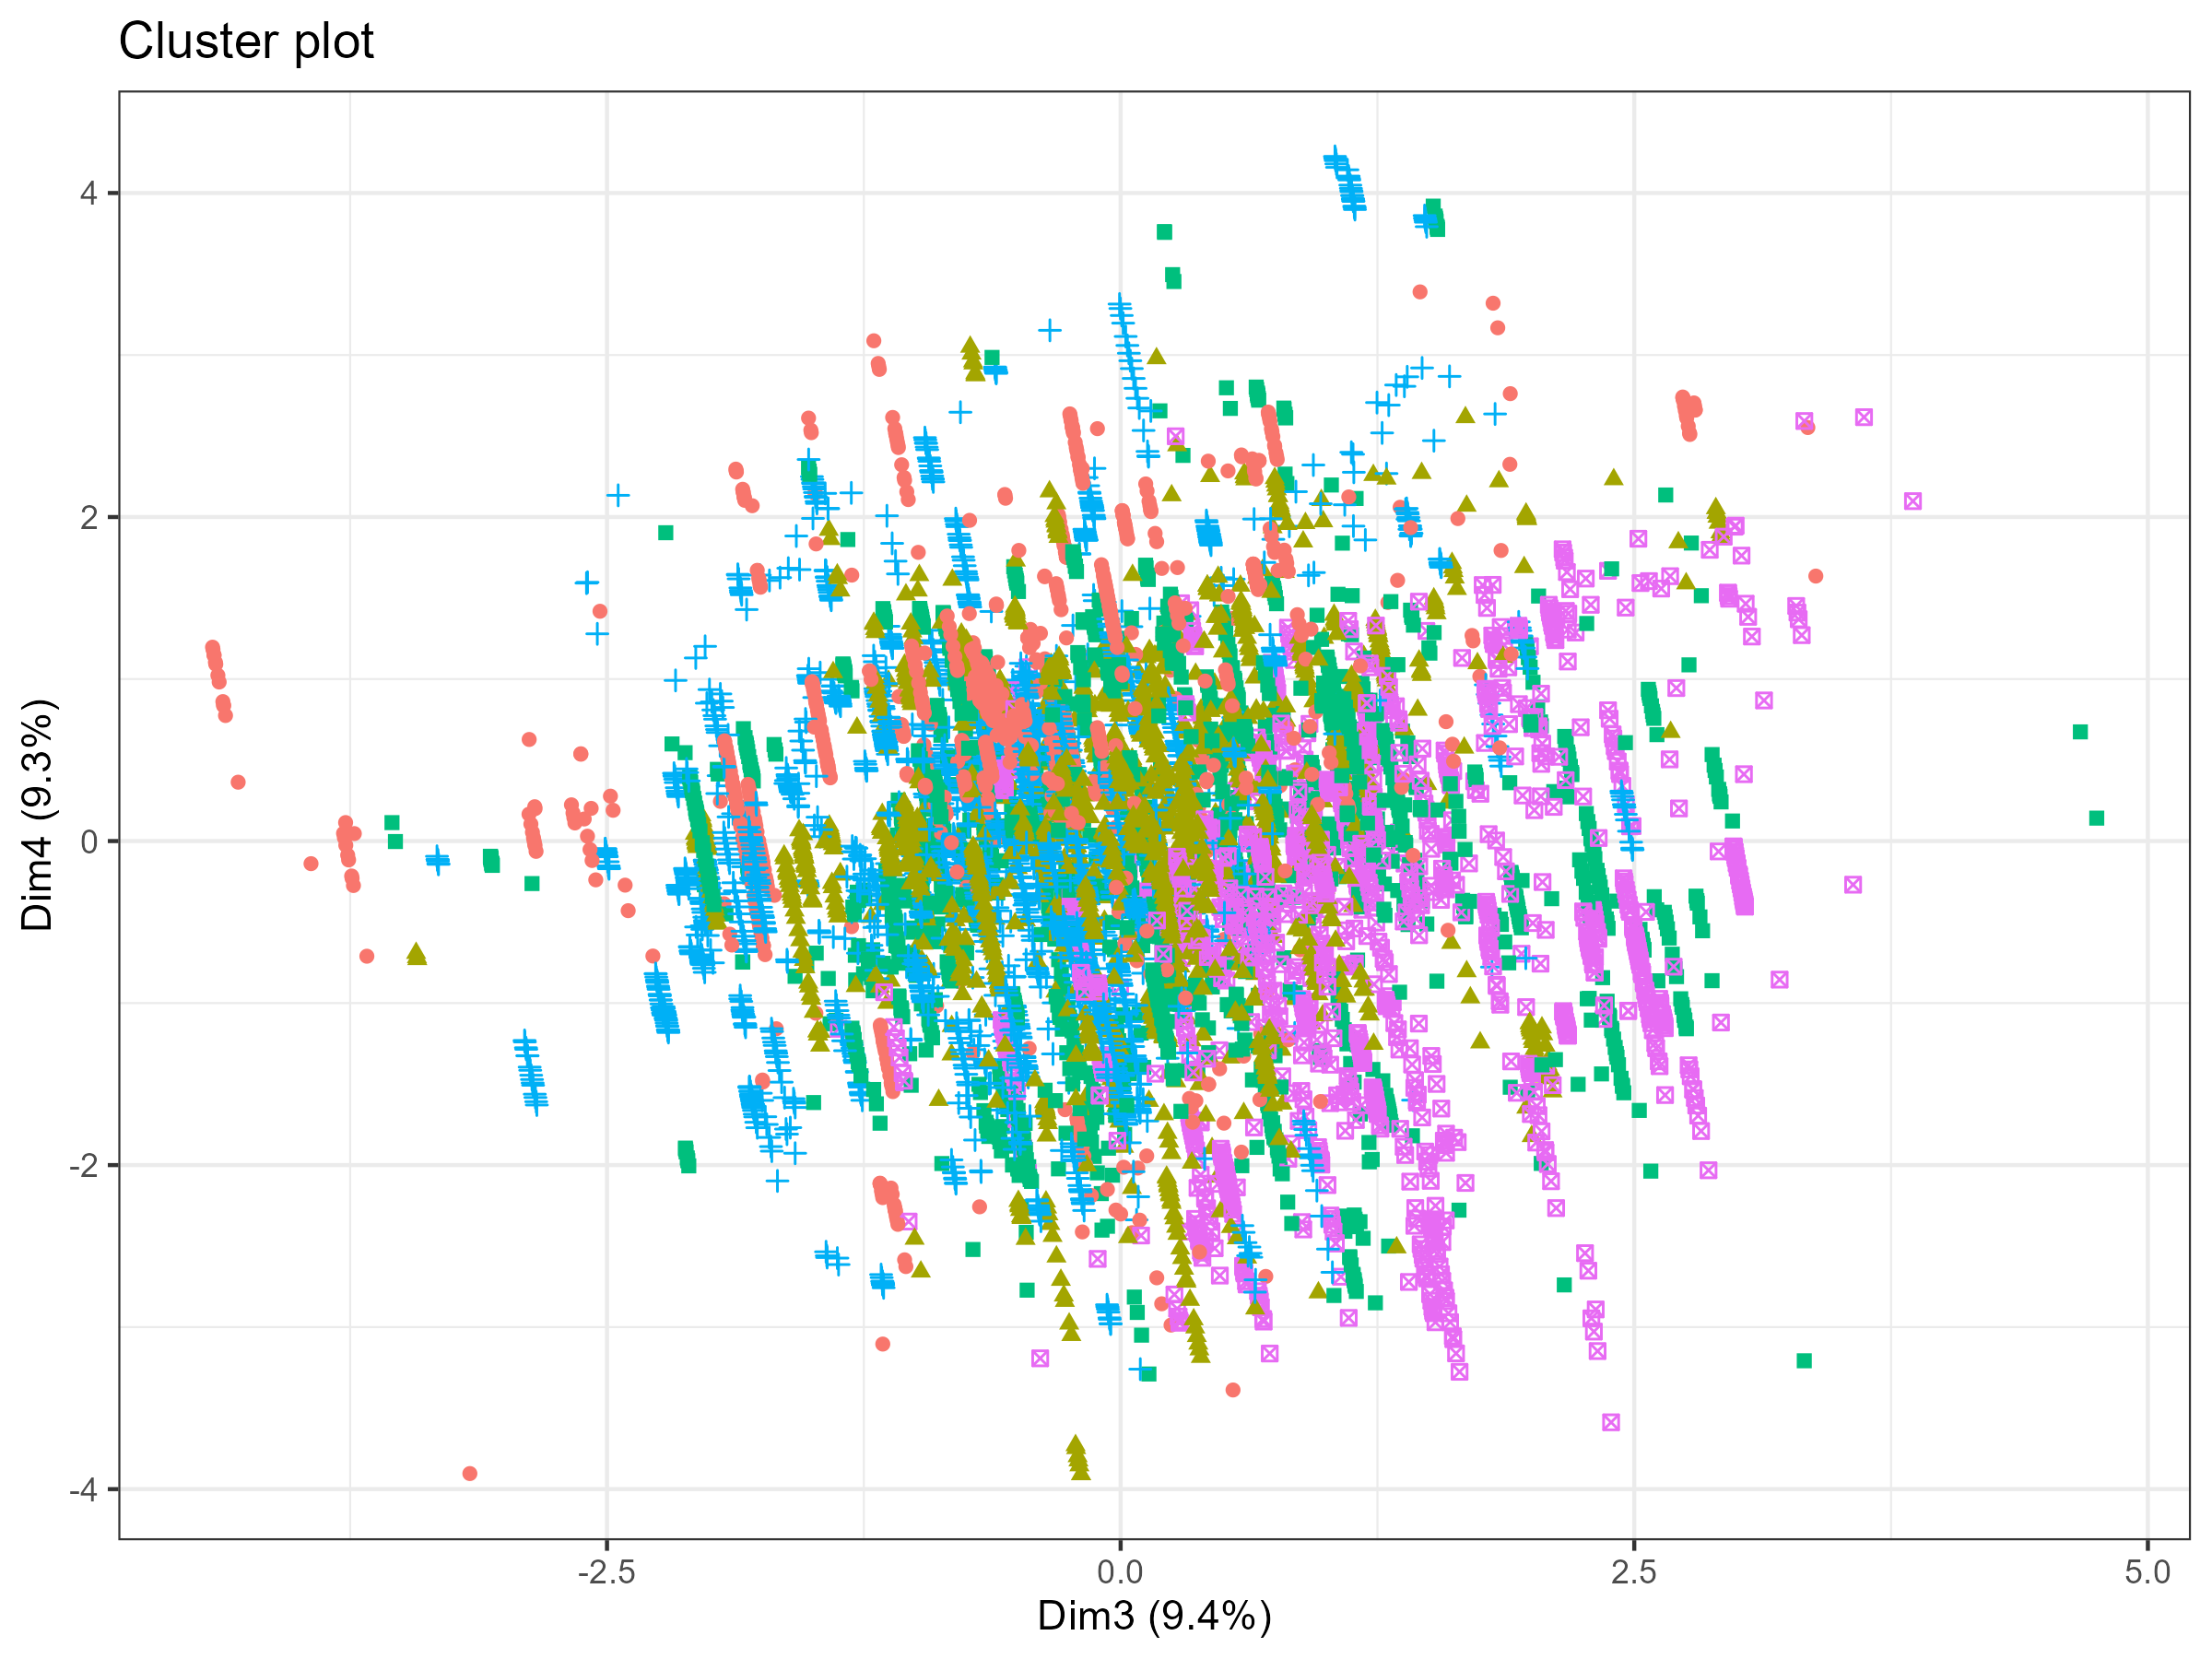
\includegraphics[width=0.8\textwidth]{Images/4_clustering/DBSCAN/kmeans34.png}
    \caption{Resultats del clústering usant K-MEANS visualitzats en components principals 3 i 4}
    \label{fig:KMEANS_34}
\end{figure}

Passant ja al DBSCAN, l’inicial (figura \ref{fig:DBSCAN_inicial}) realitzat amb 0.15 de espsilon i minPts 20 senyalava la gran majoria de punts com outliers, representats com a punts negres transparents. A més, creava molts clústers però molt petits (més de 100 clústers).

\begin{figure}[H]
    \centering
    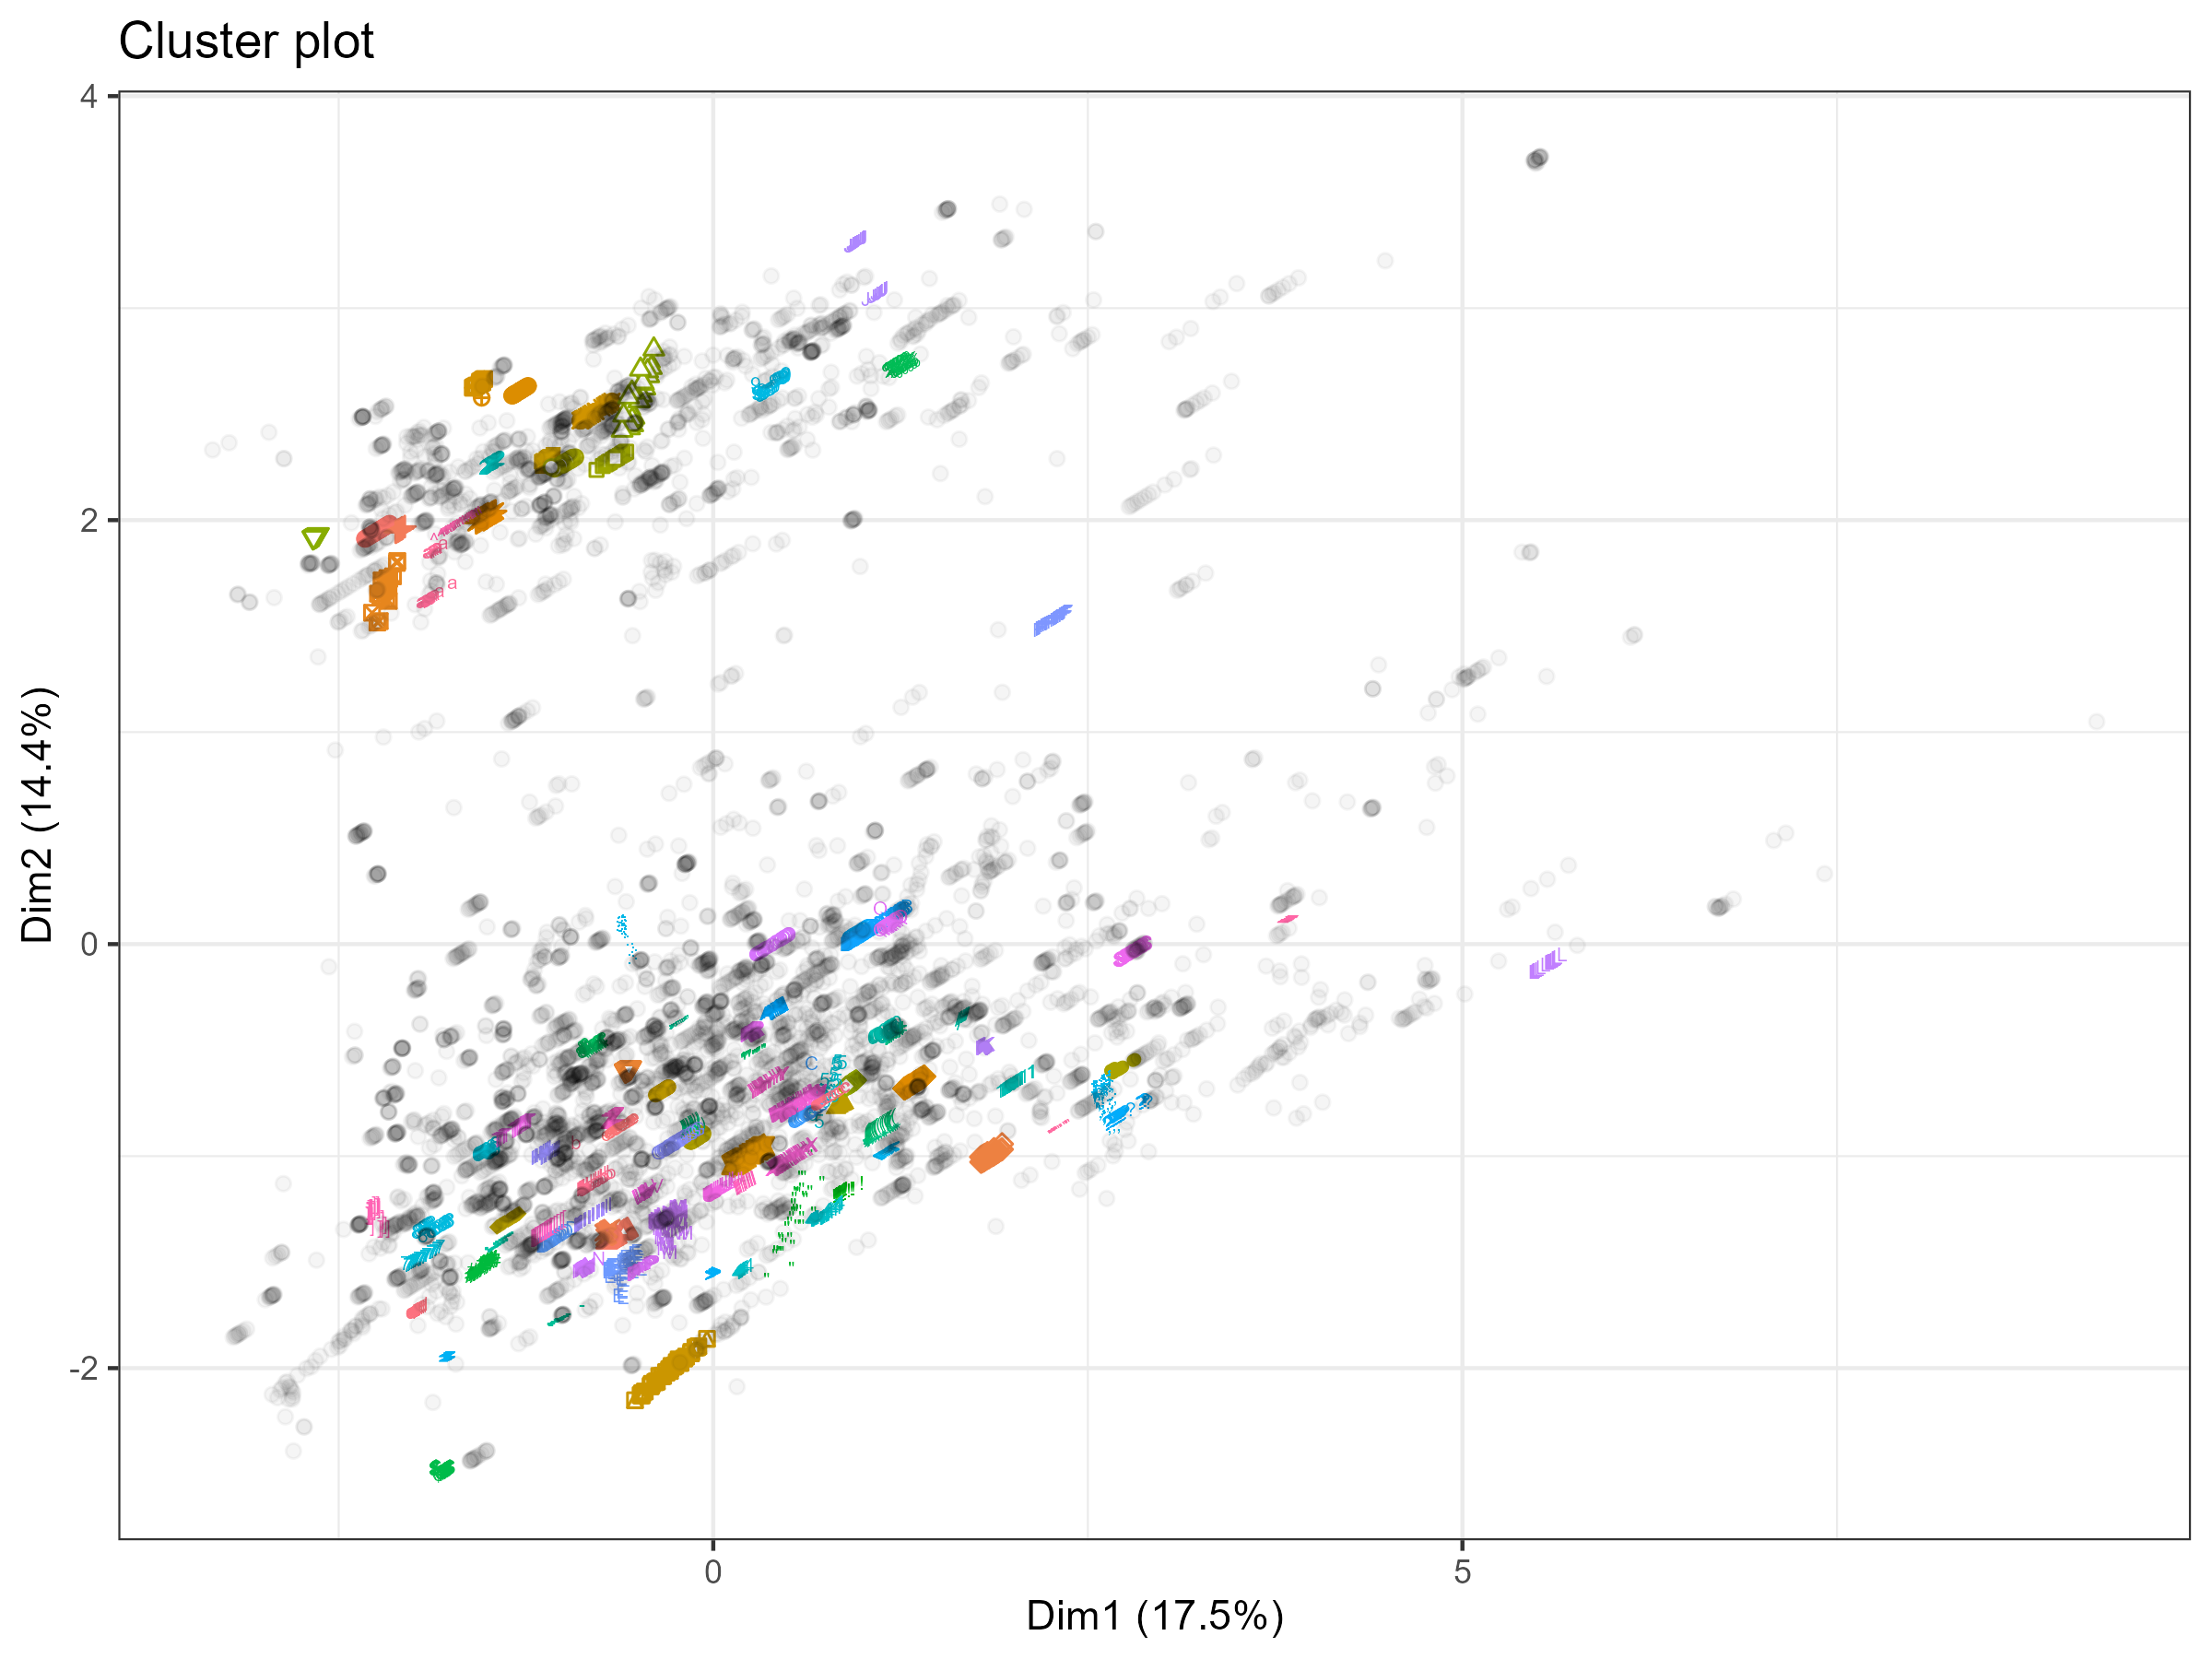
\includegraphics[width=0.8\textwidth]{Images/4_clustering/DBSCAN/baddbscan.png}
    \caption{Resultats del clústering inicial usant DBSCAN (0.15, 20) visualitzats en els dos primers components principals \\
    Des d'aquest punt tots els clústerings seran visualitzats d'aquesta manera.}
    \label{fig:DBSCAN_inicial}
\end{figure}


Per millorar els resultats, calia trobar la millor epsilon i el millor mínim de punts. Pel mínim de punts, es va escollir el 0.25\%, en aquest cas 22 punts. És un valor gran, però cal tenir en compte que la nostra base de dades també és bastant gran, amb 8800 observacions. Per escollir la epsilon, s'han realitzat les distàncies de knn, i s'ha intentat escollir el que tenia canvi de pendent màxim. Aquest retornava una epsilon de 0.72, però analitzant el gràfic s'ha determinat que un millor valor era 0.55. Tornant a realitzar el DBSCAN obteniem la figura  (figura \ref{fig:DBSCAN_auto}):

\begin{figure}[H]
    \centering
    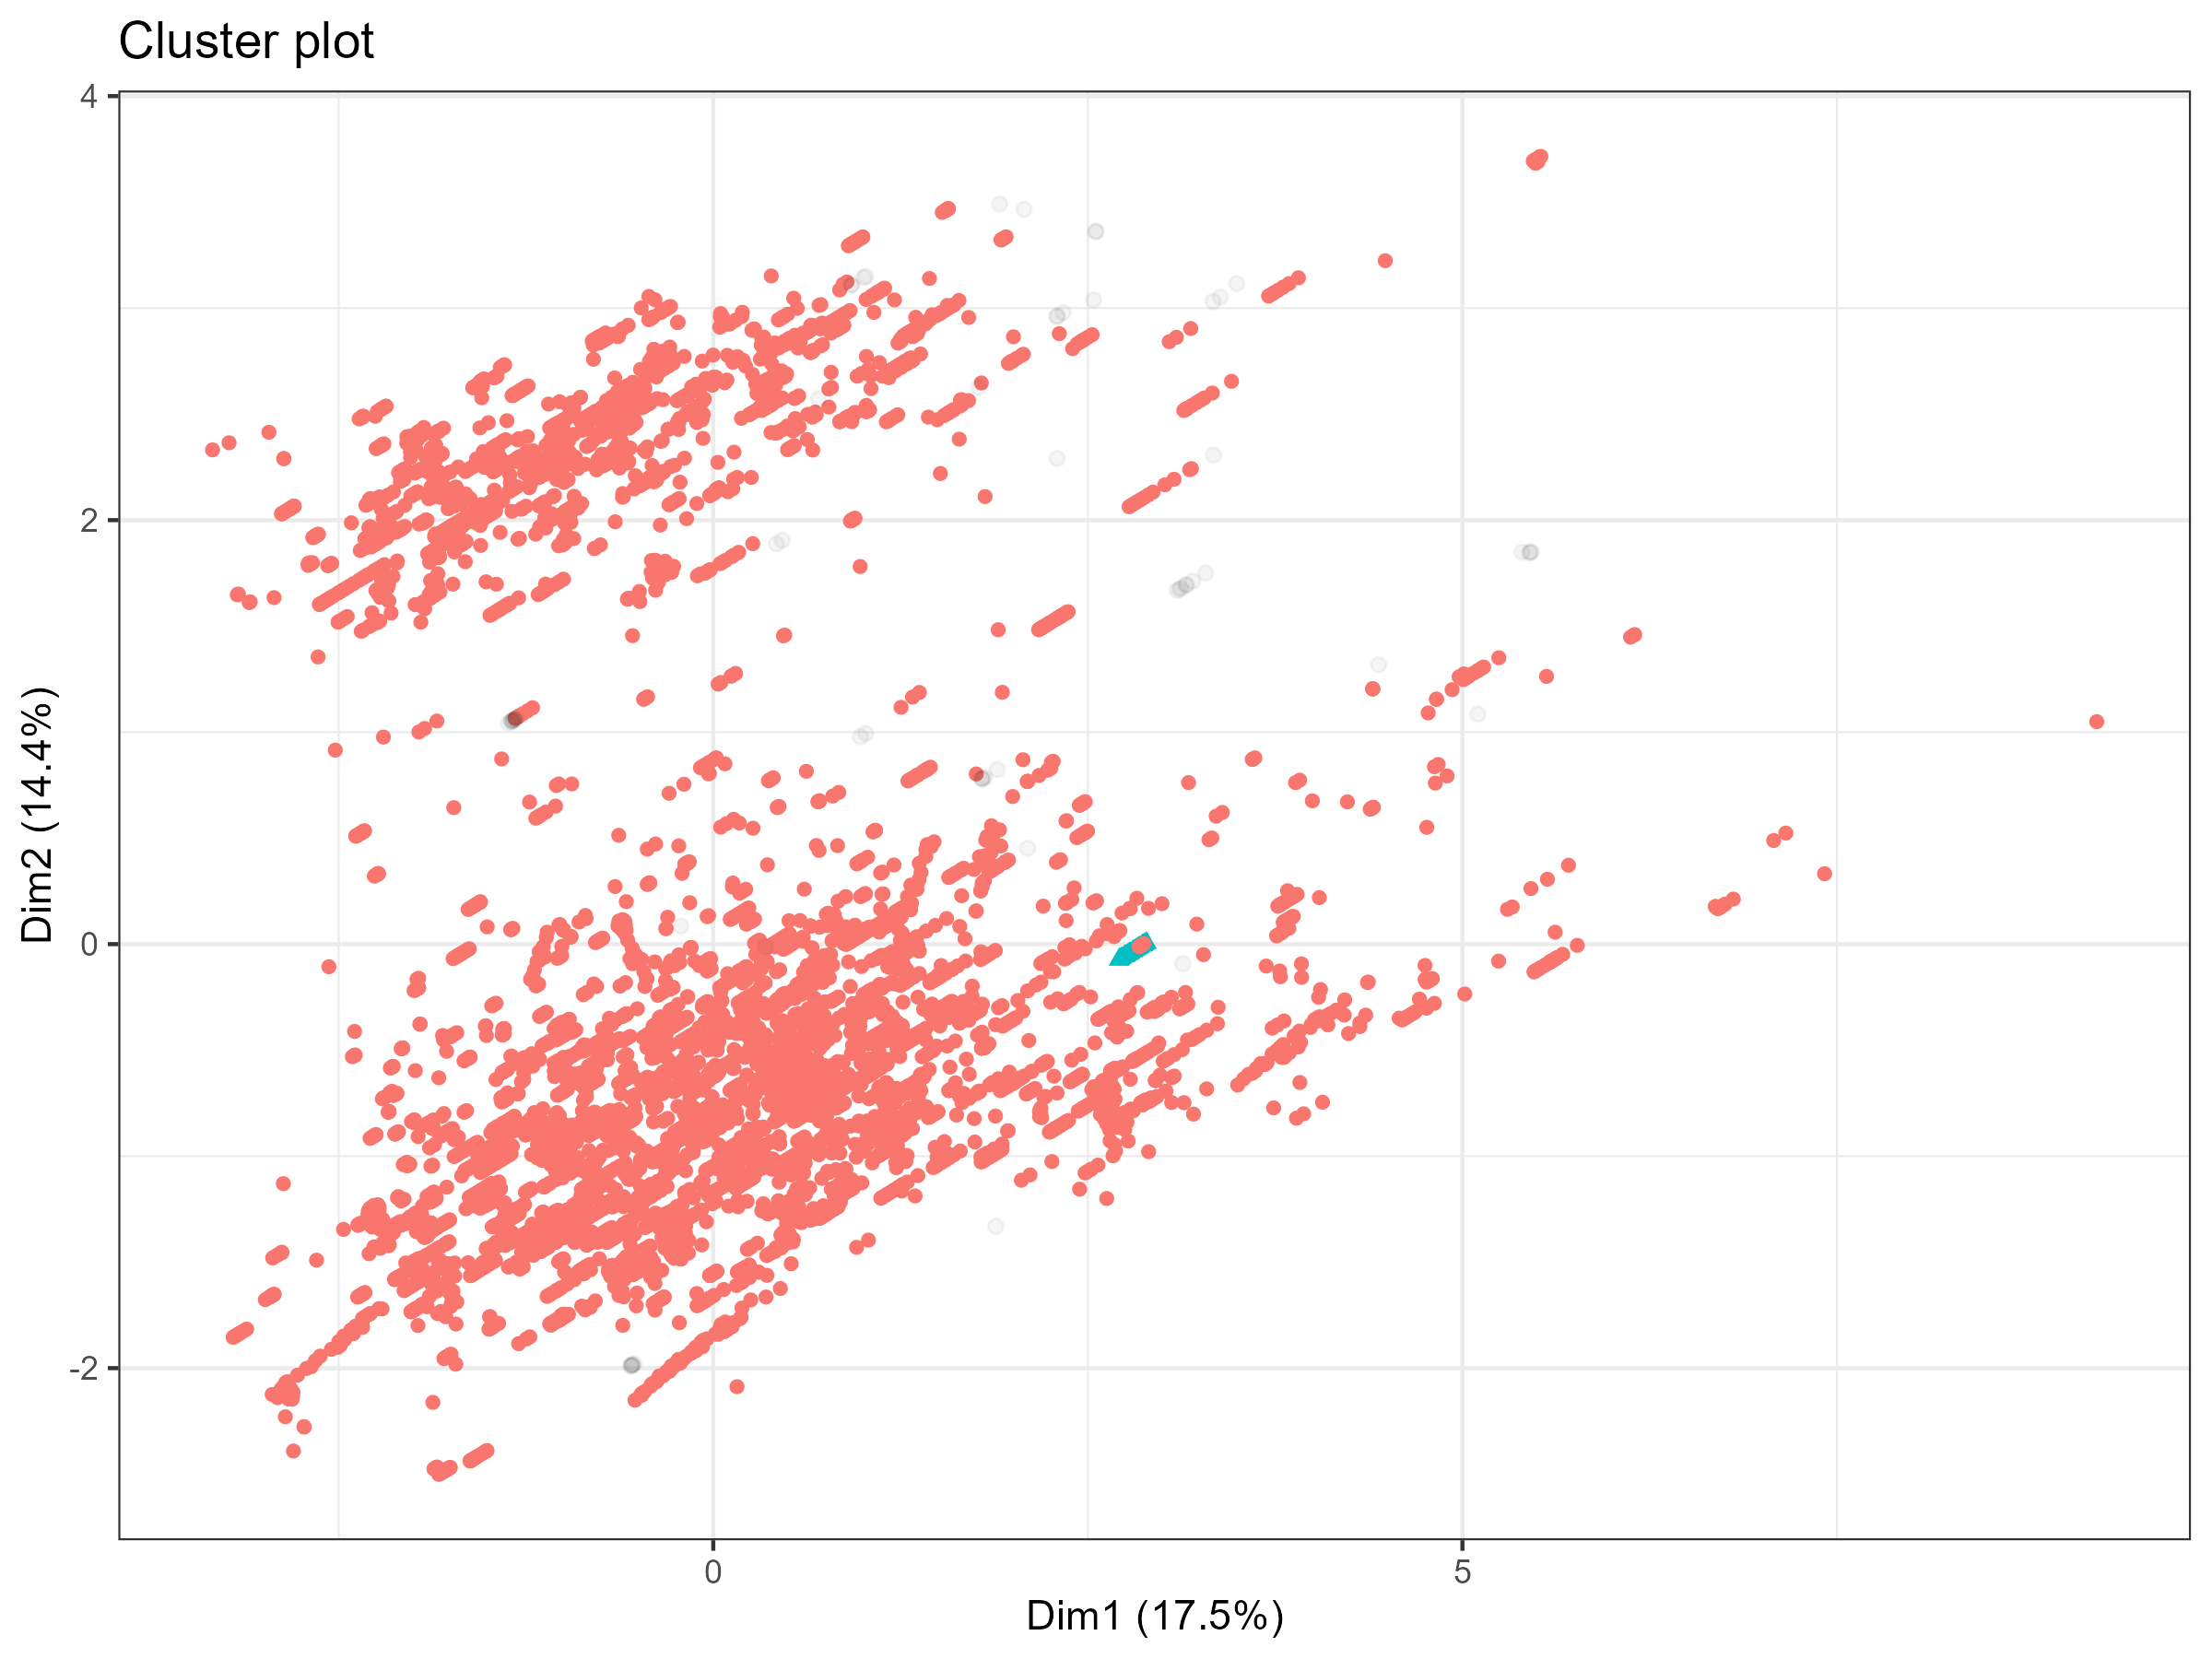
\includegraphics[width=0.8\textwidth]{Images/4_clustering/DBSCAN/dbscanauto.png}
    \caption{Resultats del clústering usant DBSCAN, epsilon knn (0.55, 22)}
    \label{fig:DBSCAN_auto}
\end{figure}

Es pot veure com aquests valors no han servit gens per millorar els resultats: ara, enlloc d'haver-hi molts clústers petits, n'hi ha un de molt gran. En teoria n'hi ha dos més, però son tan petits que són pràcticament imperceptibles.

Buscant de forma artificial uns valors de èpsilon i de mínim de punts, el resultat del DBSCAN ha sigut millor (figura \ref{fig:DBSCAN_manual}), tot i que no ha variat gaire respecte al k means: hem trobat els dos grans grups esmentats anteriorment. Per fer-ho, s'ha usat una epsilon de 0.4 i un mínim de punts de 70 (molt elevat). Amb valors més petits de mínim de punts, apareixien altre cop els clústers molt petits, que no aporten gaire res. Jugant amb la epsilon (per exemple, 0.35) es van obtenir alguns clústers dins del clúster gran de baix: un amb els valors més baixos de la dimensió 2, un altre amb els valors més alts de la dimensió 1 i un altre amb valors alts de les dues dimensions (figura \ref{fig:DBSCAN_manual2}). Tot i això, aquests clústers eren bastant petits.

\begin{figure}[H]
    \centering
    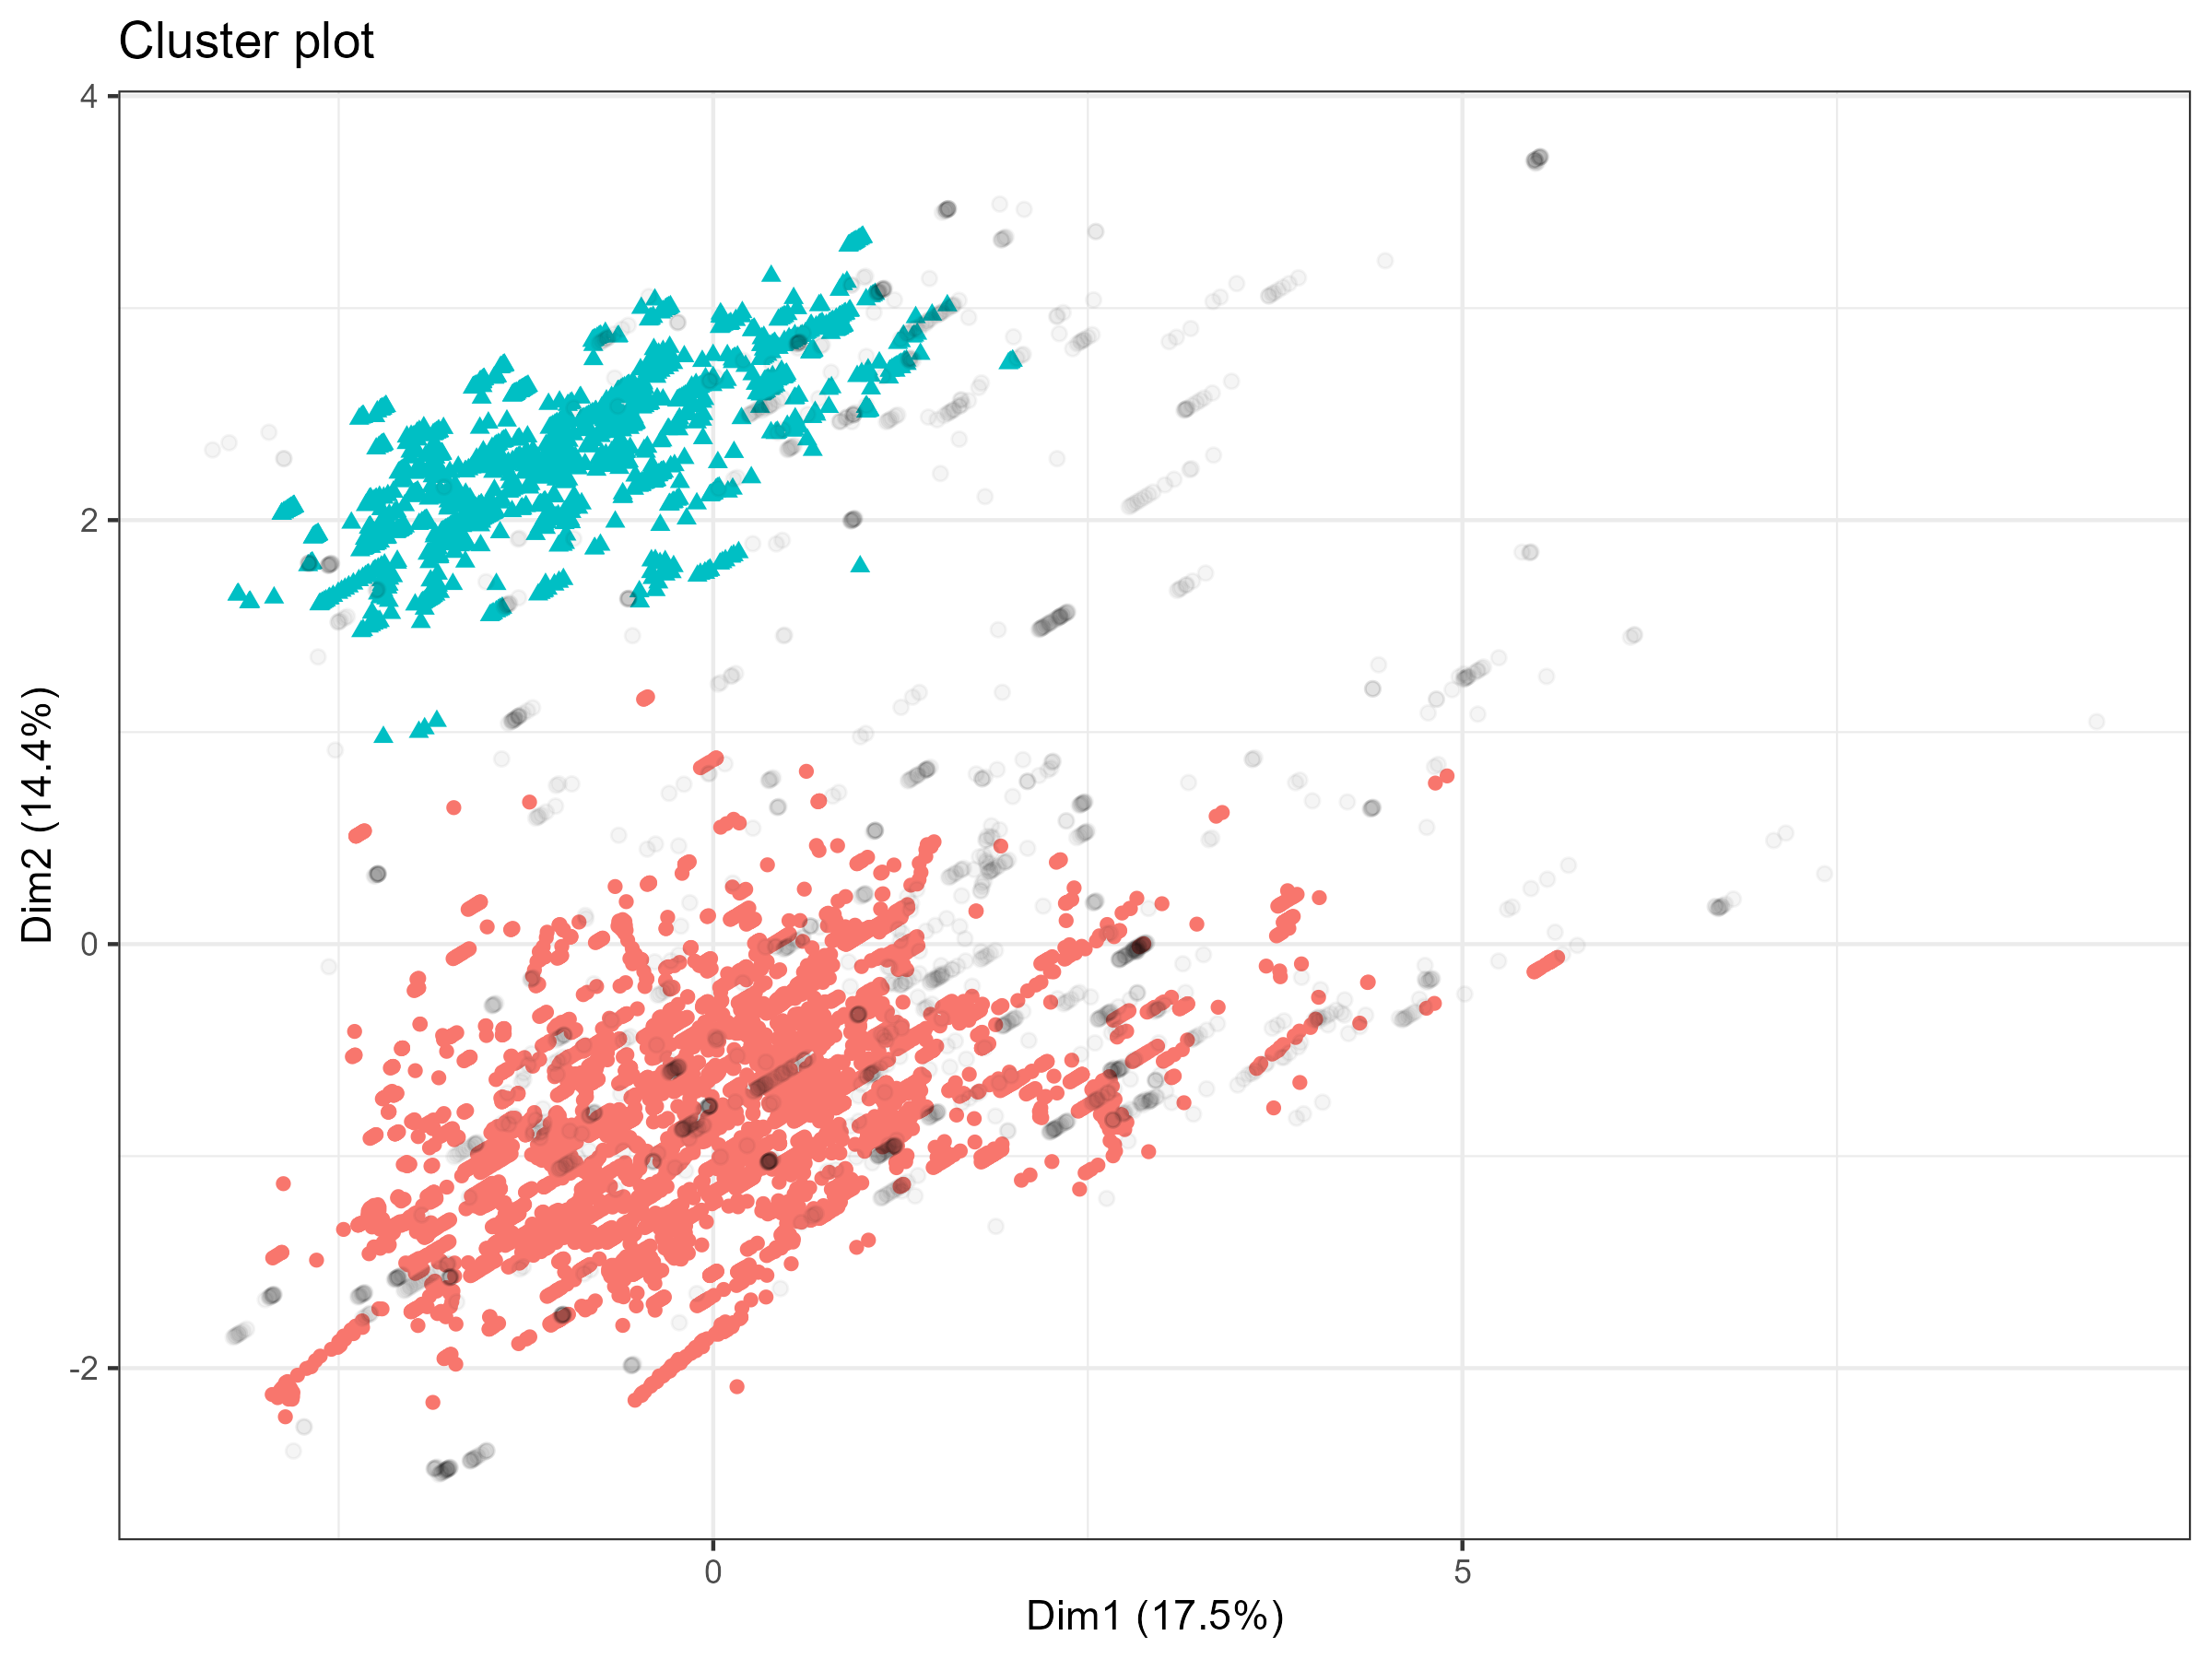
\includegraphics[width=0.8\textwidth]{Images/4_clustering/DBSCAN/dbscanforca.png}
    \caption{Resultats del clústering usant DBSCAN, epsilon manual (0.4, 70)}
    \label{fig:DBSCAN_manual}
\end{figure}

\begin{figure}[H]
    \centering
    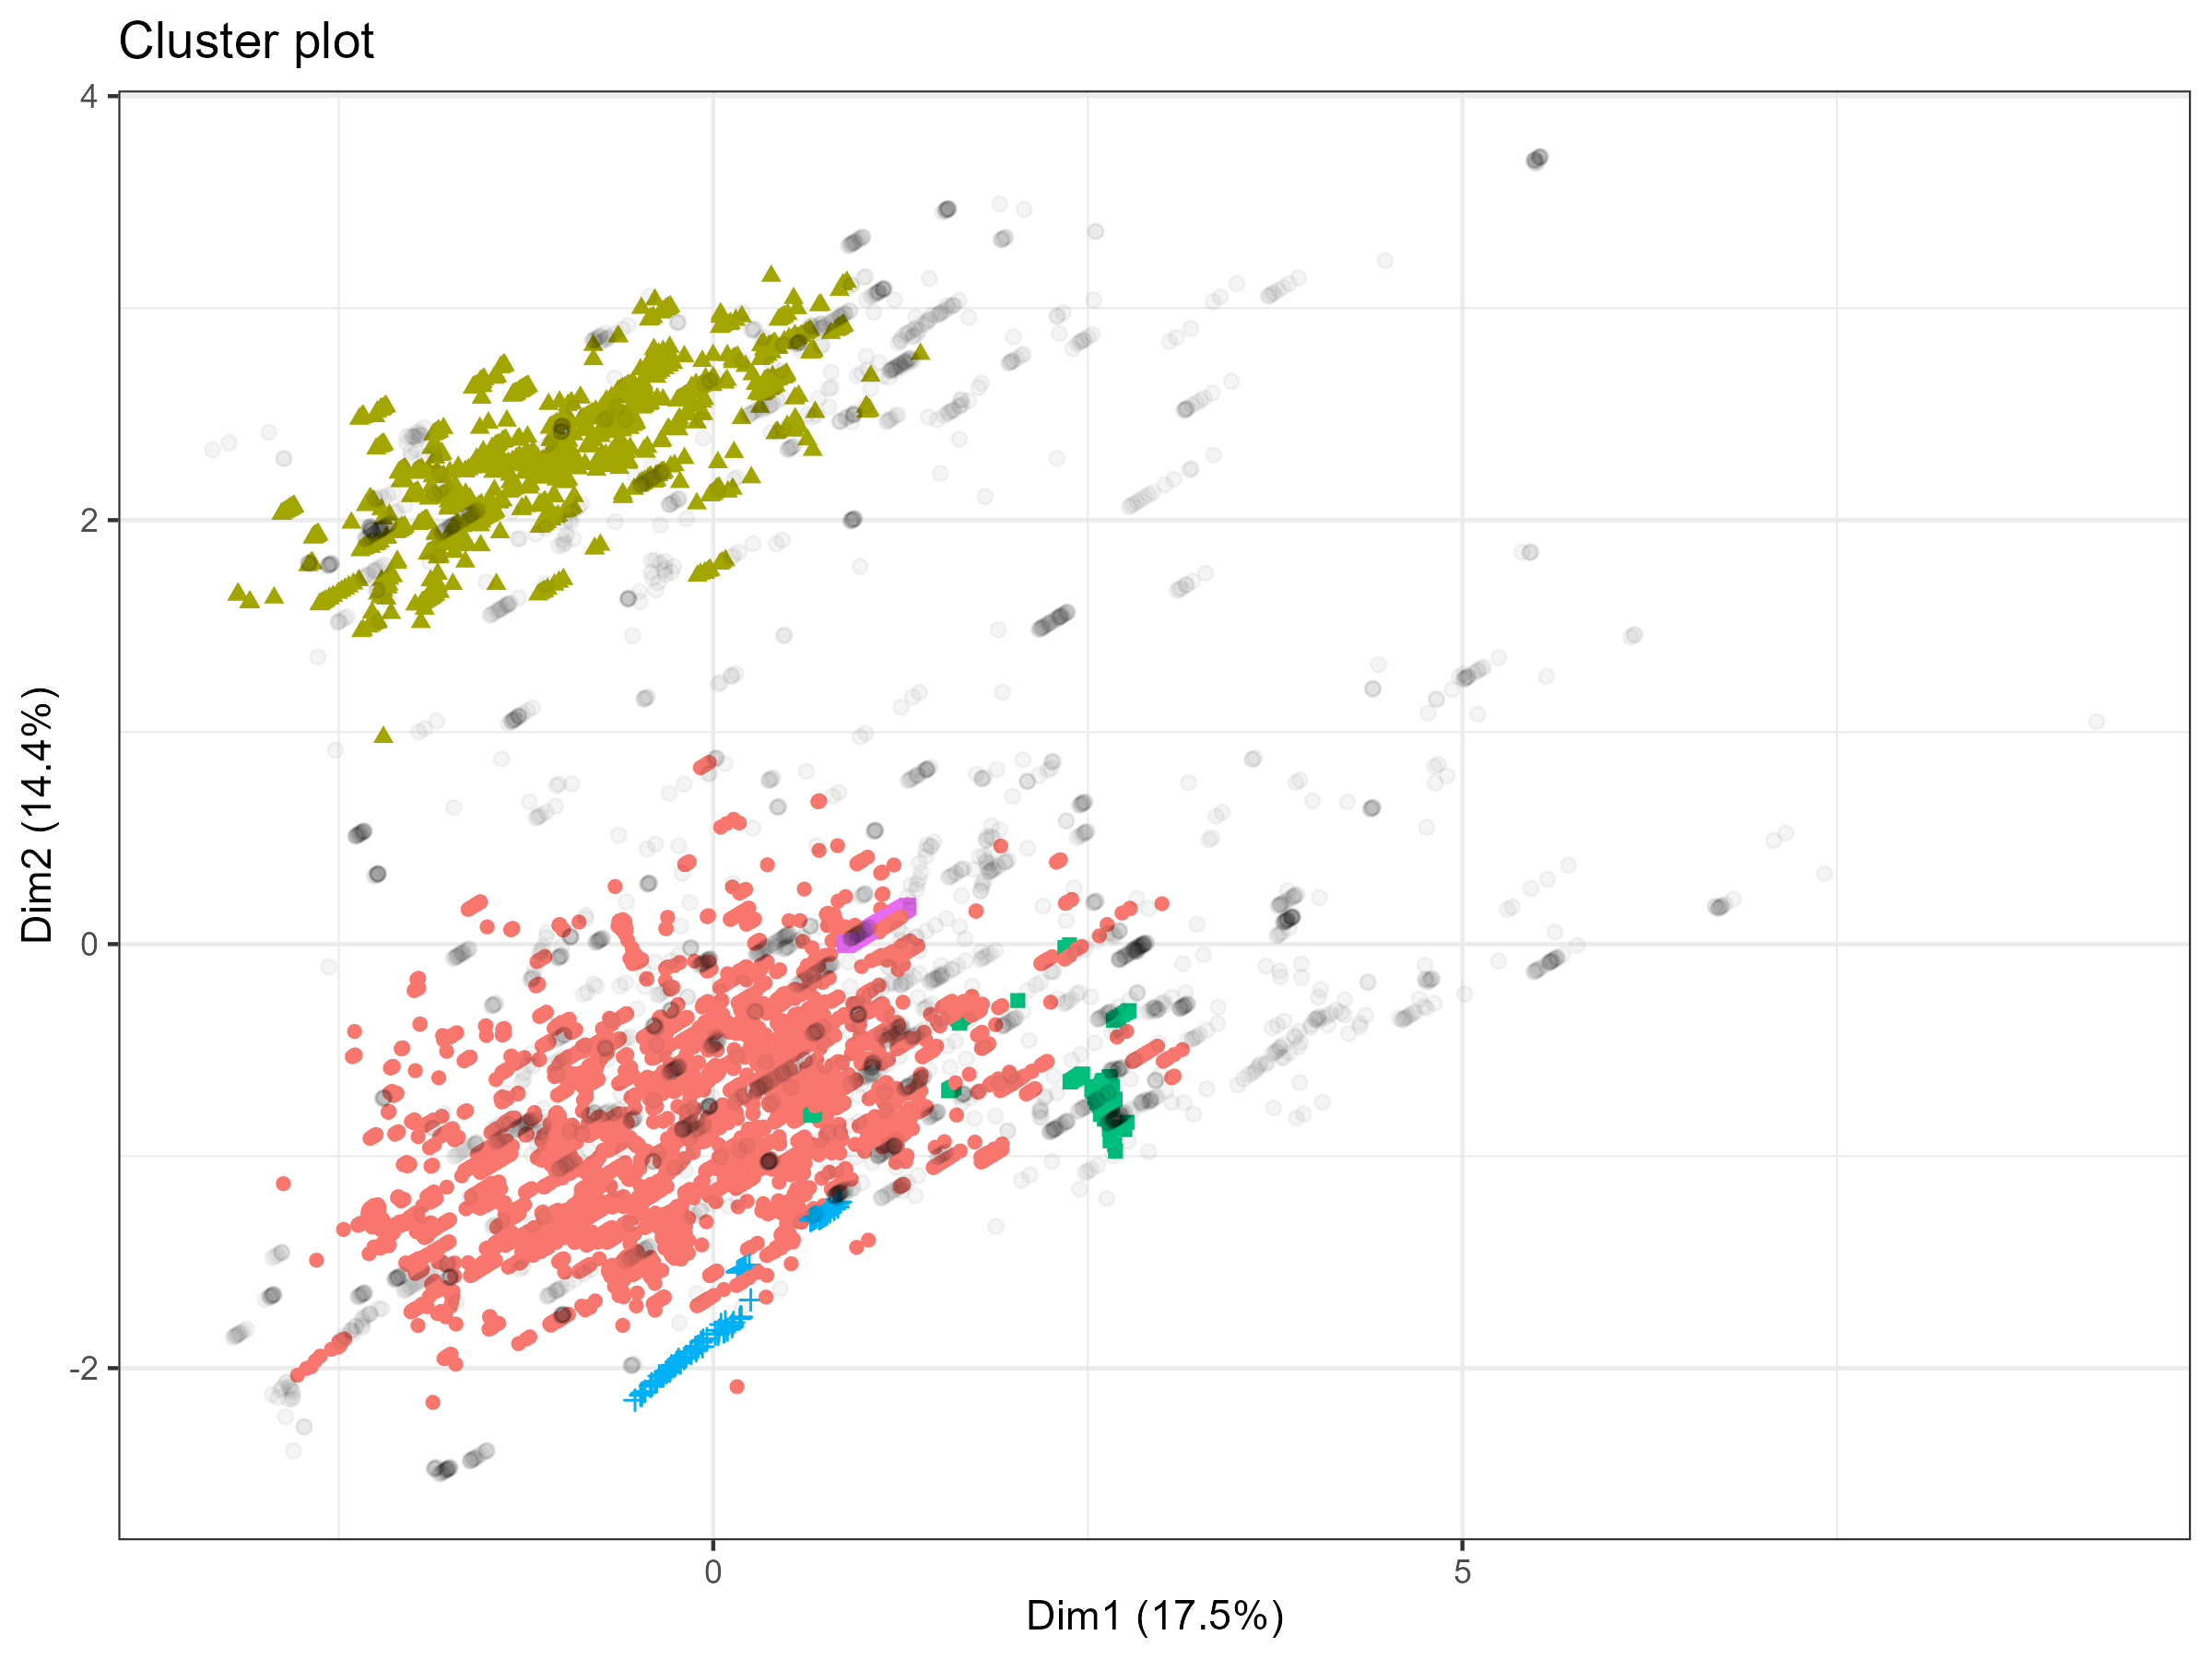
\includegraphics[width=0.8\textwidth]{Images/4_clustering/DBSCAN/dbscanforcaalt.png}
    \caption{Resultats del clústering usant DBSCAN, epsilon manual v2 (0.35, 70)}
    \label{fig:DBSCAN_manual2}
\end{figure}

En aquest apartat, el clústering escollit després de valorar totes les opcions ha sigut el DBSCAN usant epsilon 0.47 i minPts 70. Amb aquest obtenim les dues classes que s'han comentat, i 508 outliers.

A més del DBSCAN, es plantejava usar un algorisme derivat d’aquest, però que usa una tècnica diferent: OPTICS (\cite{ankerst_1999_optics}). Aquest analitza on “pot anar” cada punt, assignant-li una \textit{reachability}. En la base de dades, el reachability plot, usant els paràmetres epsilon 0.55 i minPts 22 es poden observar a la figura \ref{fig:OPTICS_inicial}.

\begin{figure}[H]
    \centering
    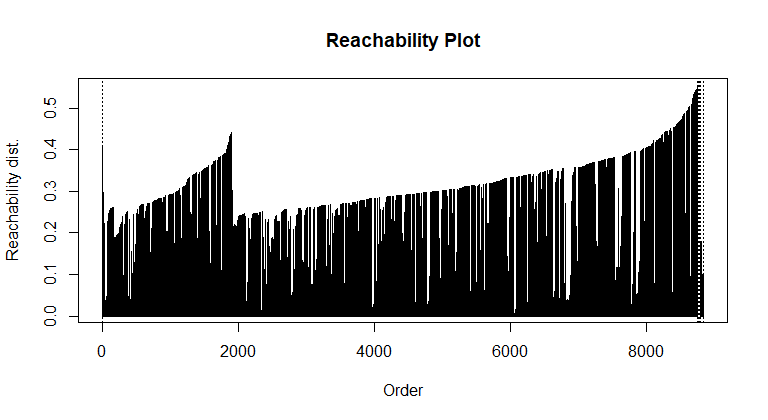
\includegraphics[width=0.8\textwidth]{Images/4_clustering/optics/reachability1.png}
    \caption{Reachability de OPTICS inicial (0.55, 22)}
    \label{fig:OPTICS_inicial}
\end{figure}

Per tal d'escollir un altre epsilon i minPts que anés millor, s'ha provat utilitzant un Grid Search tots els epsilon entre 0.1 i 1 de 0.05 en 0.05 i tots els minPts entre 10 i 70 de 10 en 10. Després d'aquesta cera, els millors valors escollits han estat 0.9 i 10 punts. El Reachability plot queda, tallant a 0.4, tal que (figura \ref{fig:OPTICS_grid}):

\begin{figure}[H]
    \centering
    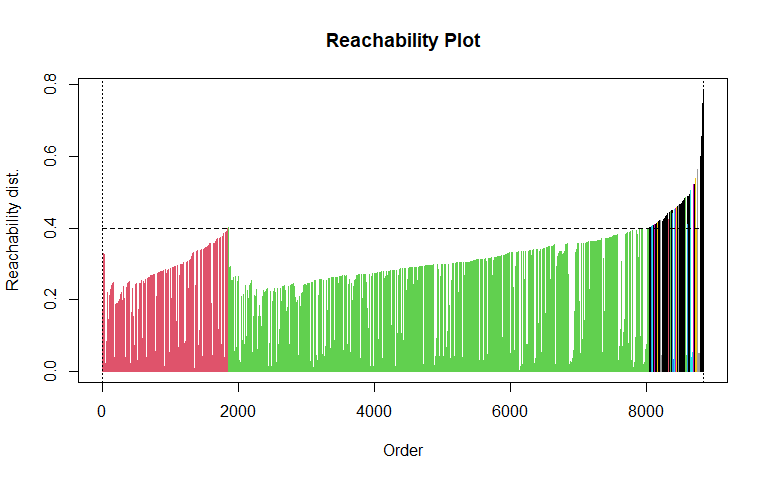
\includegraphics[width=0.8\textwidth]{Images/4_clustering/optics/reachabilitygrid.png}
    \caption{Reachability de OPTICS usant grid search (0.9, 10)}
    \label{fig:OPTICS_grid}
\end{figure}

D'aquí, podem extreure un clústering que es pot visualitzar igual que feiem amb el DBSCAN (figura \ref{fig:OPTICS_grid_res}).

\begin{figure}[H]
    \centering
    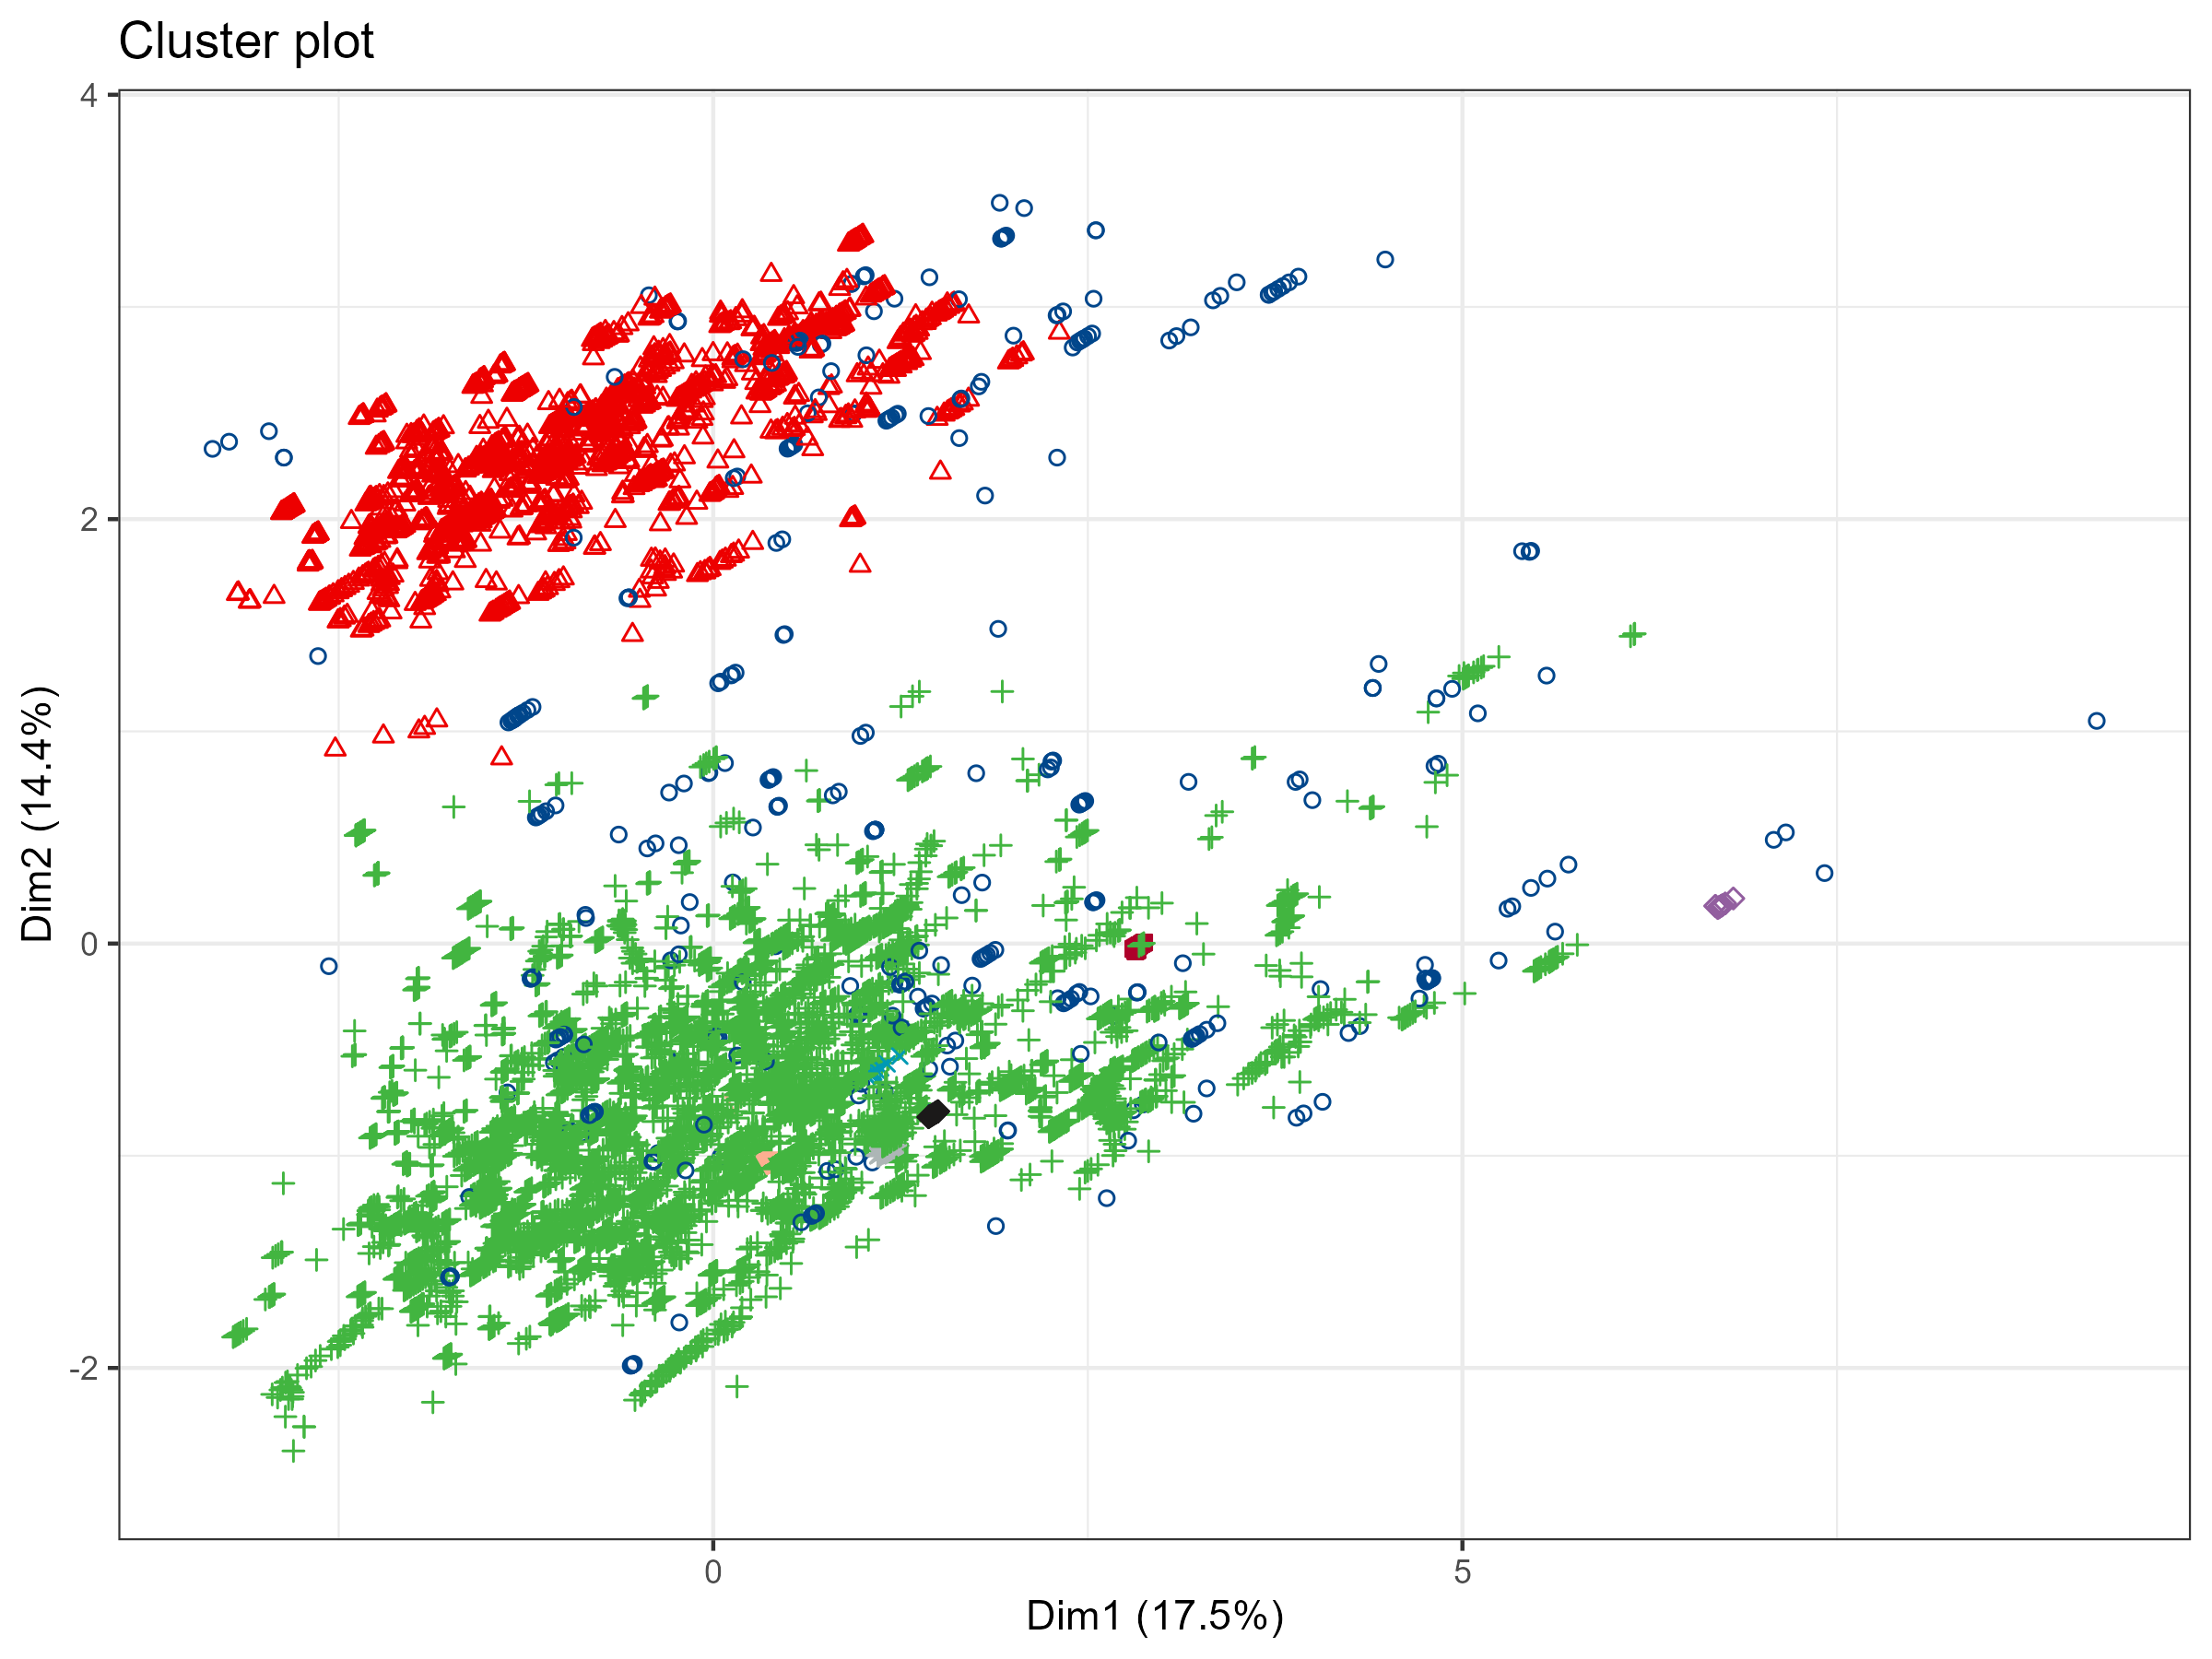
\includegraphics[width=0.8\textwidth]{Images/4_clustering/optics/opticsgrid.png}
    \caption{Resultats del clústering usant OPTICS, grid search (0.9, 10)}
    \label{fig:OPTICS_grid_res}
\end{figure}


S'observen dos clústers principals (tot i que realment n'hi ha uns 20). També veiem bastants outliers (en total 792) i clústers petits al sector dret, similar als que veiem amb el DBSCAN. L'alternativa a aquest gridSearch era usar el silhouette, però no dóna bons resultats en aquest cas, creant més de 300 clústers diferents (figura \ref{fig:OPTICS_silo}).
\begin{figure}[H]
    \centering
    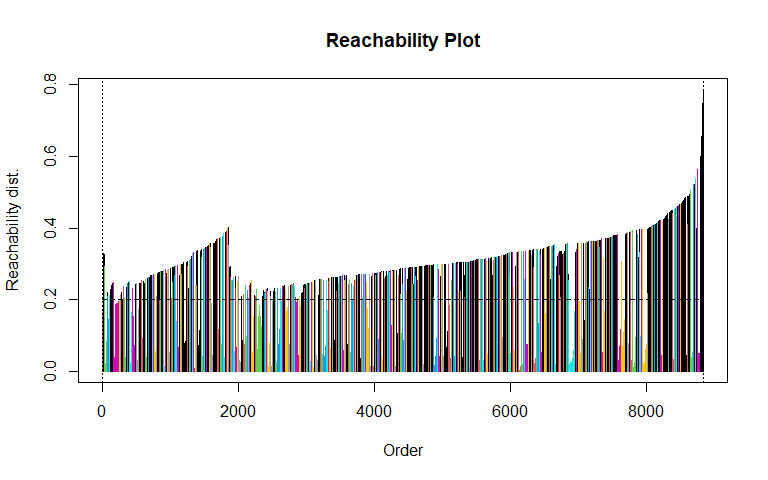
\includegraphics[width=0.8\textwidth]{Images/4_clustering/optics/siloreachability.png}
    \caption{Reachability de OPTICS usant silhouette (0.2, 22)}
    \label{fig:OPTICS_silo}
\end{figure}

En conclusió, sembla ser que l'optics no és una bona tècnica de clústering per aquestes dades. Com a molt, és capaç d'acostar-se als resultats obtinguts amb el DBSCAN. En general, les dues tècniques no han sigut capaces de crear clústers lo suficientment interessants i equilibrats com per poder extreure'n bona informació, o sigui que probablement no siguin les millors per aquestes dades. En aquest cas, el KMEANS creava uns clústers més interessants, i encara que no detectés outliers, probablement serien agrupacions més interessants.


\subsection{Clústering de sèries temporals}

S'ha realitzat una anàlisi de clústering de sèries temporals per a les cançons més escoltades mensualment a Spotify entre els anys 2017 i 2021. L'objectiu ha estat identificar patrons de comportament en les tendències de streams, que poden revelar agrupacions de cançons amb trajectòries similars en el temps, incloent hits ràpids o cançons amb una presència sostinguda en el temps.

Per dur a terme aquesta anàlisi, primer s'han carregat i preparat les dades, transformant-les per adequar-se a l'anàlisi de sèries temporals. Aquesta preparació ha inclòs la transformació de les variables \texttt{year\_week} i \texttt{month\_week} en una única columna de text per al mes i any, així com la pivotació de les dades per tenir aquesta nova variable \texttt{year\_month} en columnes i \texttt{track\_name} en files. Per a cada valor de fila i columna es va fer una agregació de totes les reproduccions de la cançó en aquell mes en concret.

S'ha seleccionat la variable \texttt{streams} per a l'anàlisi, considerant que aquesta proporcionaria el major benefici per a l'empresa al analitzar les cançons amb tendències de popularitat ràpida o sostinguda. S'ha prestat molta atenció al fet que, degut a que les dades només inclouen les cançons que estan dins del top 40 global de Spotify, les streams d'una cançó en un mes on no apareix cap vegada s'han considerat com a 0. Aquesta aproximació s'ha justificat amb l'ús de la Distància Temporal Dinàmica (DTW) per al càlcul de similituds, entenent que els valors 0 tenen menys pes en la comparació, i per tant, l'anàlisi es centra més en les tendències presents que en les absències.

Amb les dades preparades, s'ha realitzat un clústering jeràrquic utilitzant la distància DTW i el mètode de Ward. Aquest mètode s'ha escollit per la seva capacitat de crear grups basats en la minimització de la variància dins dels clústers, ideal per identificar grups de cançons amb patrons de streams similars al llarg del temps. 

Després de l'anàlisi jeràrquic, s'ha realitzat el dendrograma per poder escollir quin és el nombre més adequat de classes.

\begin{figure}[H]
    \centering
    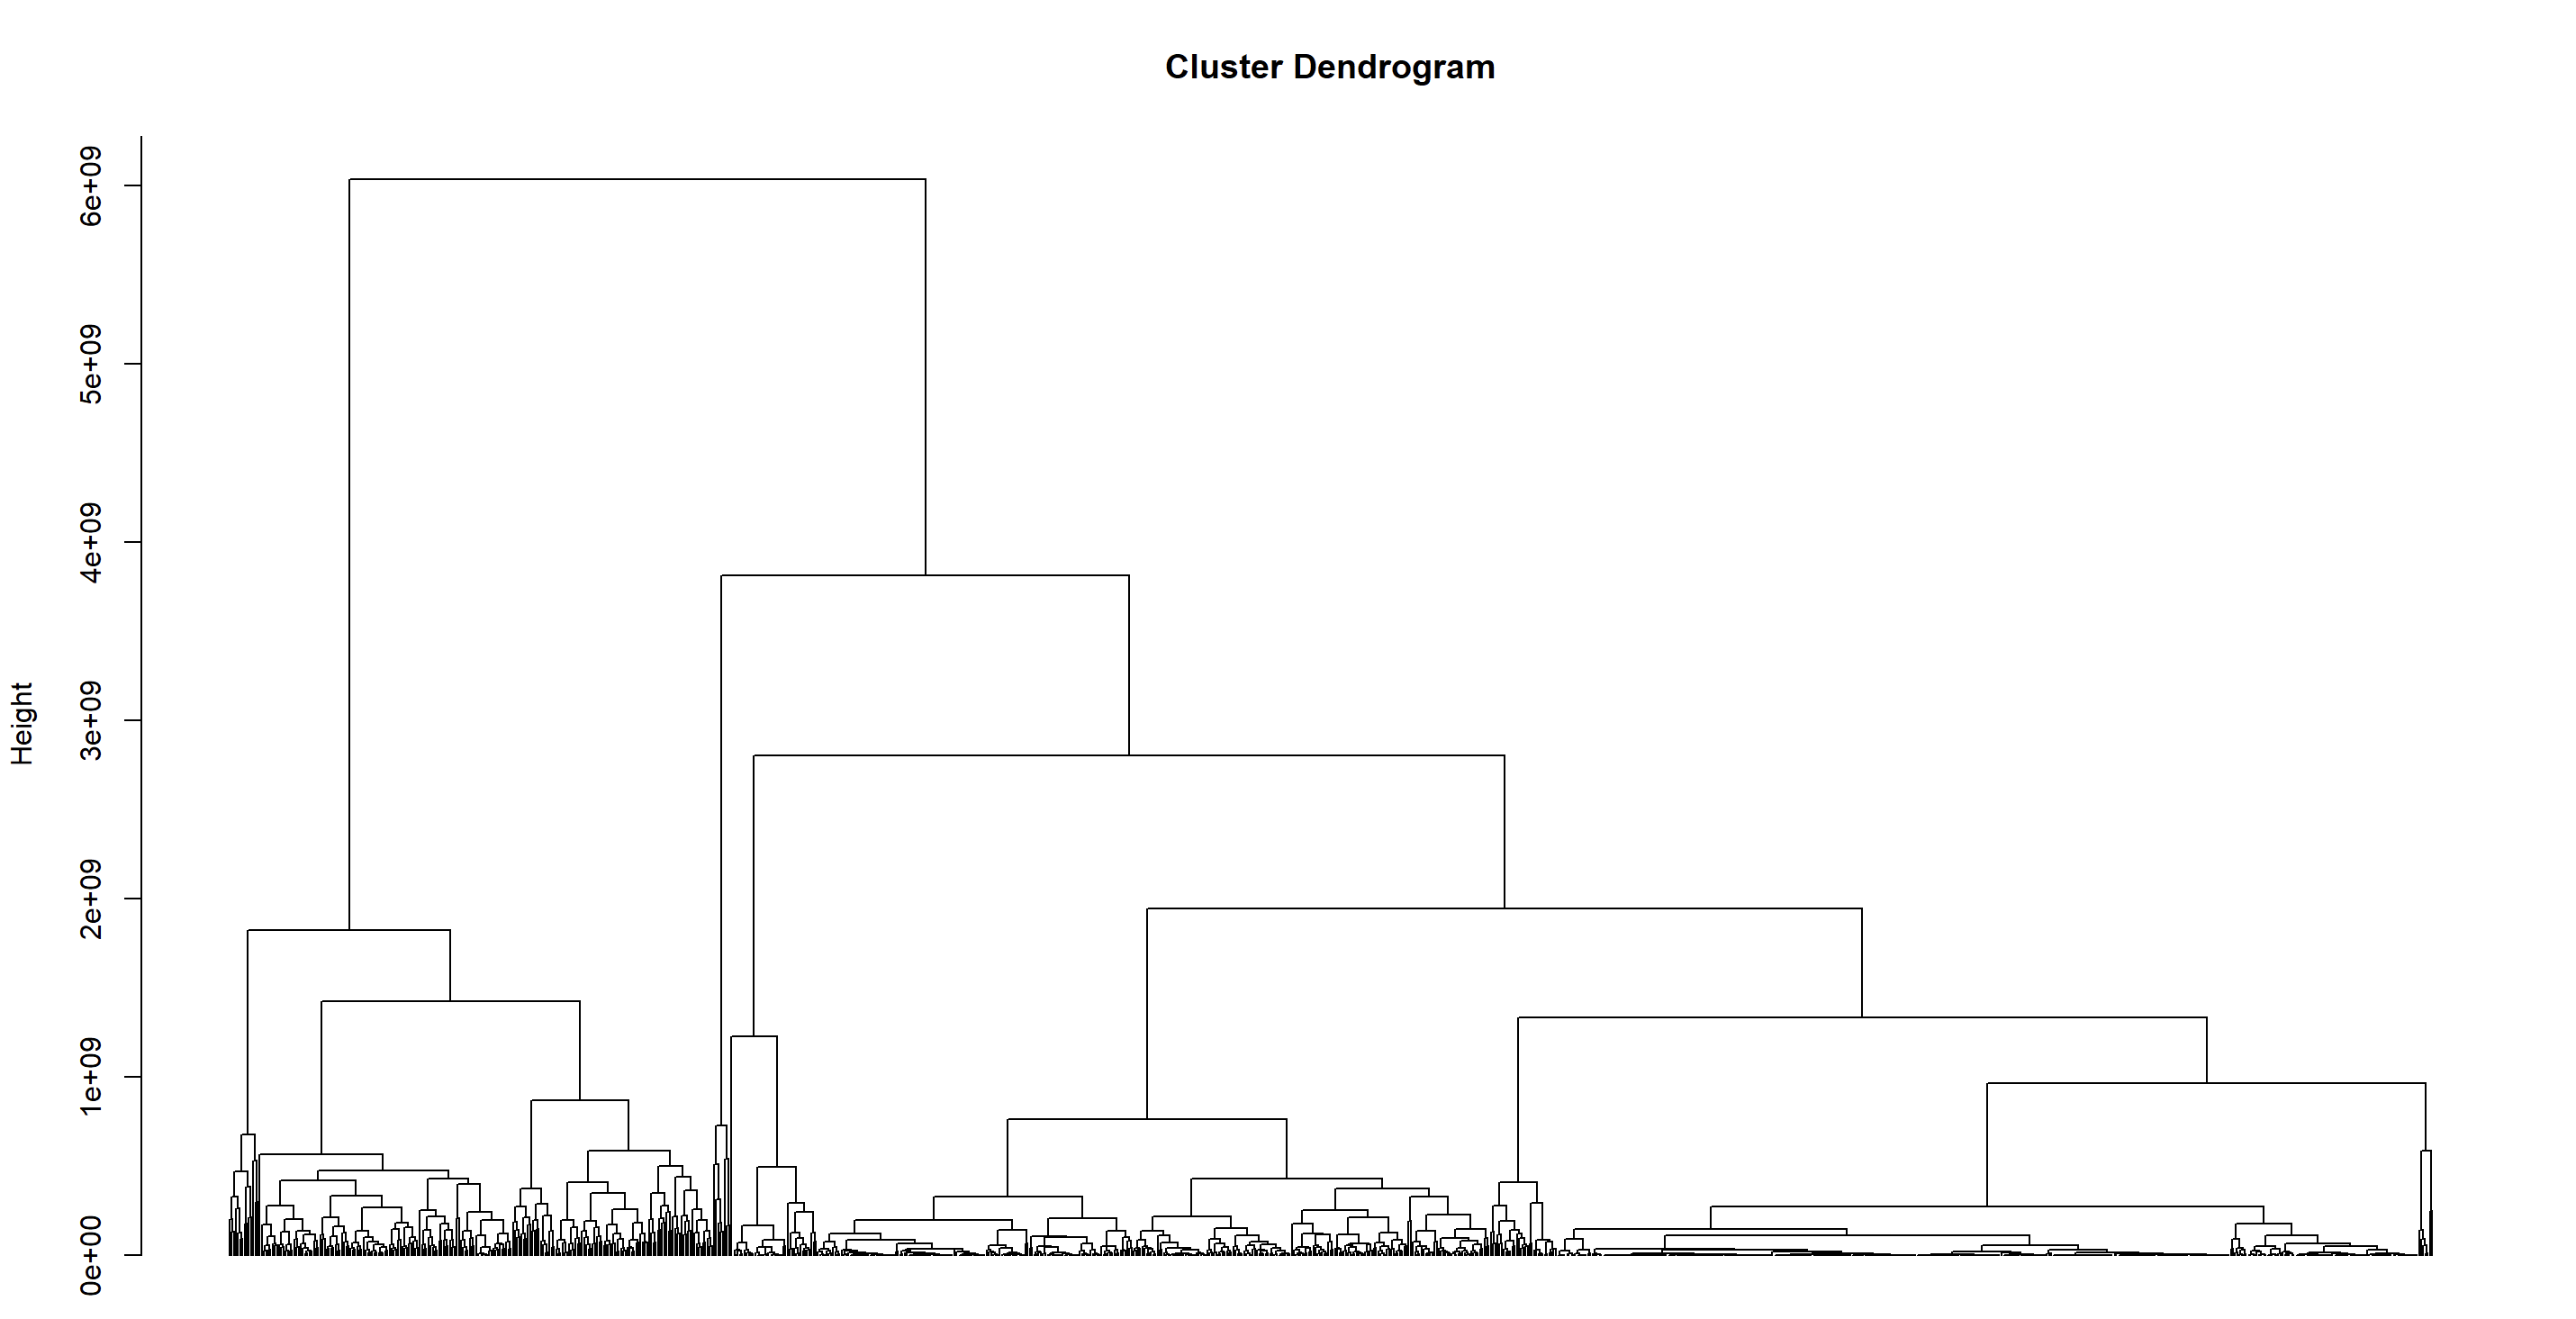
\includegraphics[width=\textwidth]{Images/4_clustering/time_series/dendrograma_original.png}
    \caption{Dendrograma de cançons utilitzant distància \texttt{DTW} i mètode \texttt{ward.D2}}
    \label{fig:TS_dendrograma_original}
\end{figure}

Com es pot veure en la figura \ref{fig:TS_dendrograma_original} el nombre \textit{k} a escollir no és gaire evident degut al desbalanceig de la majoria de clústers. Després d'analitzar aquest equilibri de classes, s'ha realitzat un tall per obtenir 5 classes diferents per tal d'intentar tenir una quantitat de cançons similar a tots els clústers (intentant mantenir una \textit{k} petita igualment).

Com es pot veure en la següent taula \ref{tab:TS_clustering_results} les 3 primeres classes tenen un nombre prou equilibrat de cançons mentre que en el quart n'hi ha moltes menys i en el cinquè gairebé no n'hi ha cap. Aquest fet és curiós degut a que molt probablement aquestes cançons agrupades en classes tan reduïdes podrien estar molt relacionades entre si podent arribar a conclusions interessants.

\begin{table}[H]
\centering
\begin{tabular}{|c|c|c|c|c|}
\hline
1    & 2    & 3   & 4   & 5 \\ \hline
311 & 436 & 224 & 40 & 8  \\ \hline
\end{tabular}
\caption{Resultat del clústering de les sèries temporals}
\label{tab:TS_clustering_results}
\end{table}

Una vegada s'ha escollit el valor de $k = 5$, en la figura \ref{fig:TS_dendrograma_colors} es pot veure el dendrograma colorejat per tal de visualitzar els diferents clústers. El color verd representa el clúster número 3, el color lila el 5, el blau el 4, el vermell l'1 i el mostassa el 2.

\begin{figure}[H]
    \centering
    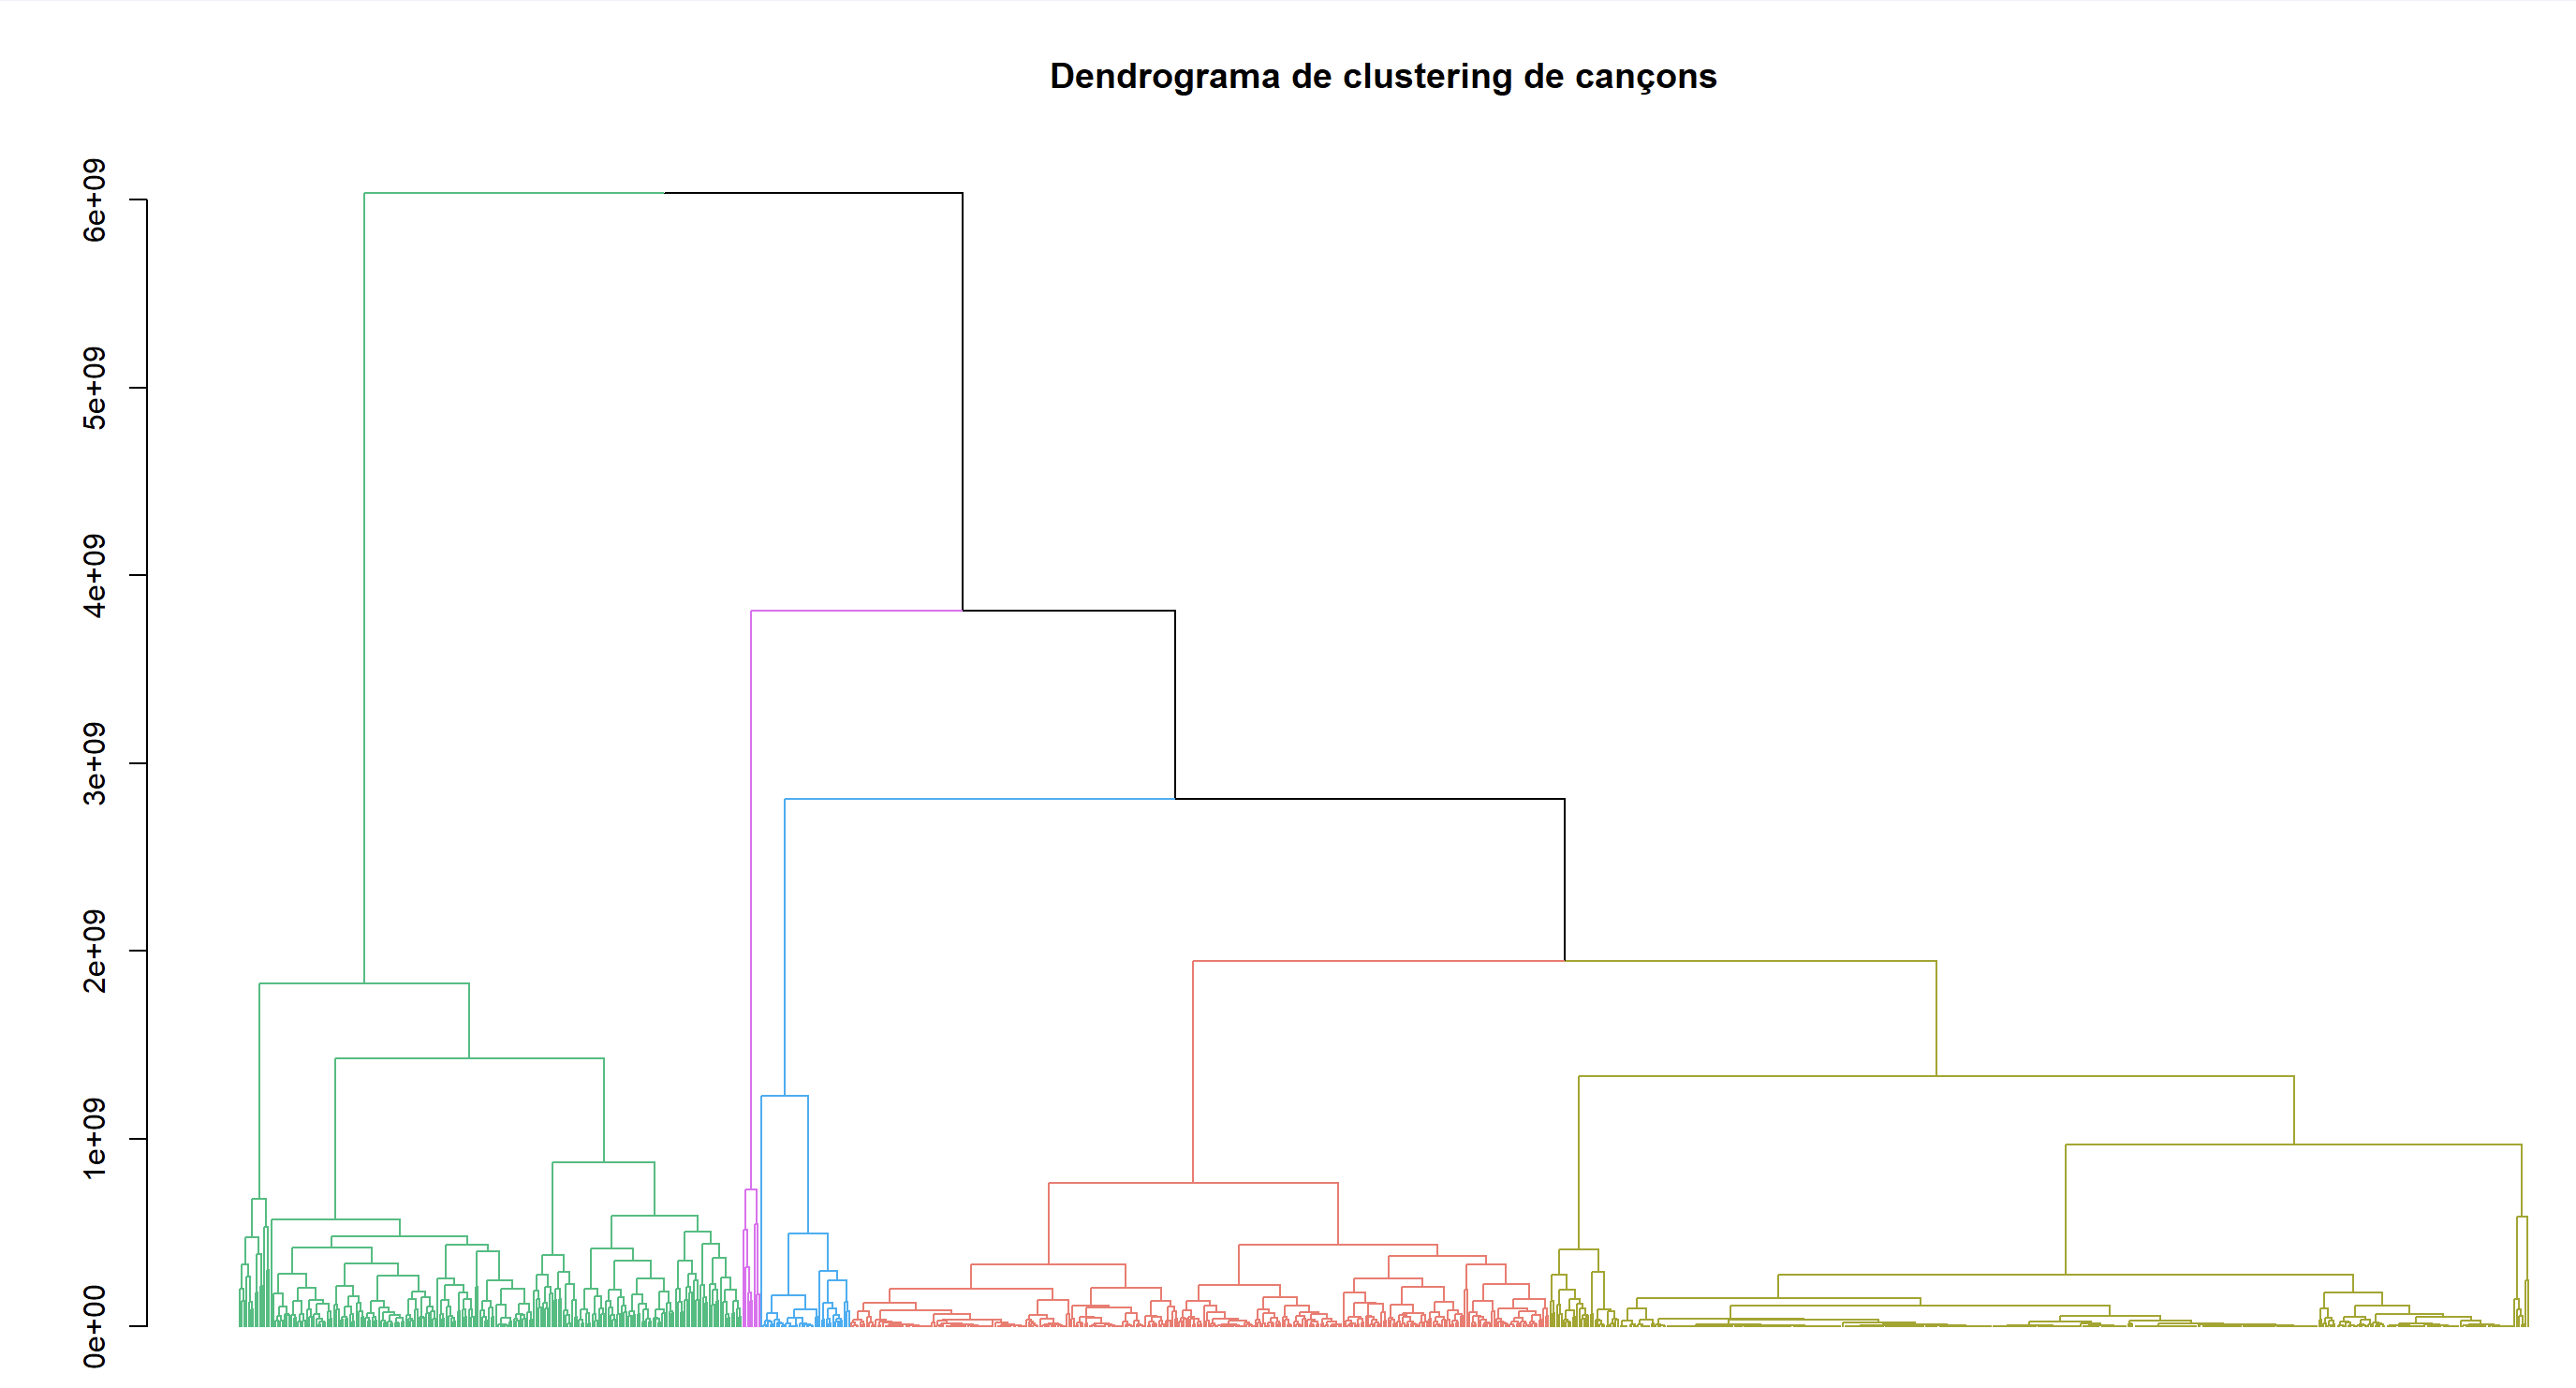
\includegraphics[width=\textwidth]{Images/4_clustering/time_series/dendrograma_colors.png}
    \caption{Dendrograma de cançons utilitzant distància \texttt{DTW} i mètode \texttt{ward.D2} amb els clústers colorejats ($k = 5$)}
    \label{fig:TS_dendrograma_colors}
\end{figure}

\subsubsection{Anàlisi dels resultats}

Amb els clústers ja establerts, s'ha procedit a realitzar un anàlisi detallat dels resultats amb l'objectiu d'interpretar i comprendre els motius subjacents que han conduït a la formació d'aquestes agrupacions

Les visualitzacions i anàlisis post-clústering, com ara la comparació entre els clústers i la durada mitjana de les cançons per cada agrupació, ofereixen una perspectiva més profunda permetent descobrir patrons amagats que ajudin a entendre millor la situació musical de l'aplicació.

Pel que fa a la figura \ref{fig:TS_tsclust_sc} podem observar les evolucions de les reproduccions per a cada clúster al llarg del temps.  Simplement al fer una breu ullada ja podem veure, més o menys, com estan distribuïdes les cançons. \\

\begin{itemize}
    \item \textbf{Clúster 1:} Aquest grup mostra un patró consistent en la quantitat de \textit{streams} amb un alt nivell de superposició de les sèries alhora que allargada, indicant una quantitat de streams sostinguda.
    
    \item \textbf{Clúster 2:} Aquest clúster presenta uns pics molt marcats al llarg dels anys indicant èxit ocasionalment que podria ser a causa de promocions o esdeveniments o inclús d'altres aplicacions que tenen molt poder d'influència com ara \textit{TikTok}. Cal recordar que la majoria de cançons es troben en aquest grup, i en aquests pics no s'hi veuen moltes cançons, de manera que hi ha una gran quantitat de cançons (les que no formen els pics) que no són tan populars i conformen la majoria del clúster.
    
    \item \textbf{Clúster 3:} Aquesta classe és molt similar al primer clúster però amb una diferència més significativa en les variacions entre cançons, encara que segueixen tenint una popularitat allargada. A més, els valors màxims són considerablement més alts que els del clúster 1, de manera que segurament hi ha cançons més populars en aquest clúster.
    
    \item \textbf{Clúster 4:} En aquest grup trobem les cançons que eren populars a l'inici de la creació del \textit{dataset} però que ràpidament van perdre l'interès, possiblement \textit{hits} d'aquella temporada. Cal mencionar com ja s'ha vist anteriorment que aquest clúster compta amb molt poques cançons, concretament 40.
    
    \item \textbf{Clúster 5:} Aquest grup, que és el més petit de tots, és el que té un període més llarg d'èxit i on les cançons tarden més en sortir del top després del pic. A més, els valors màxims són molt alts, de manera que segurament conté cançons molt populars.
\end{itemize}


\begin{figure}[H]
    \centering
    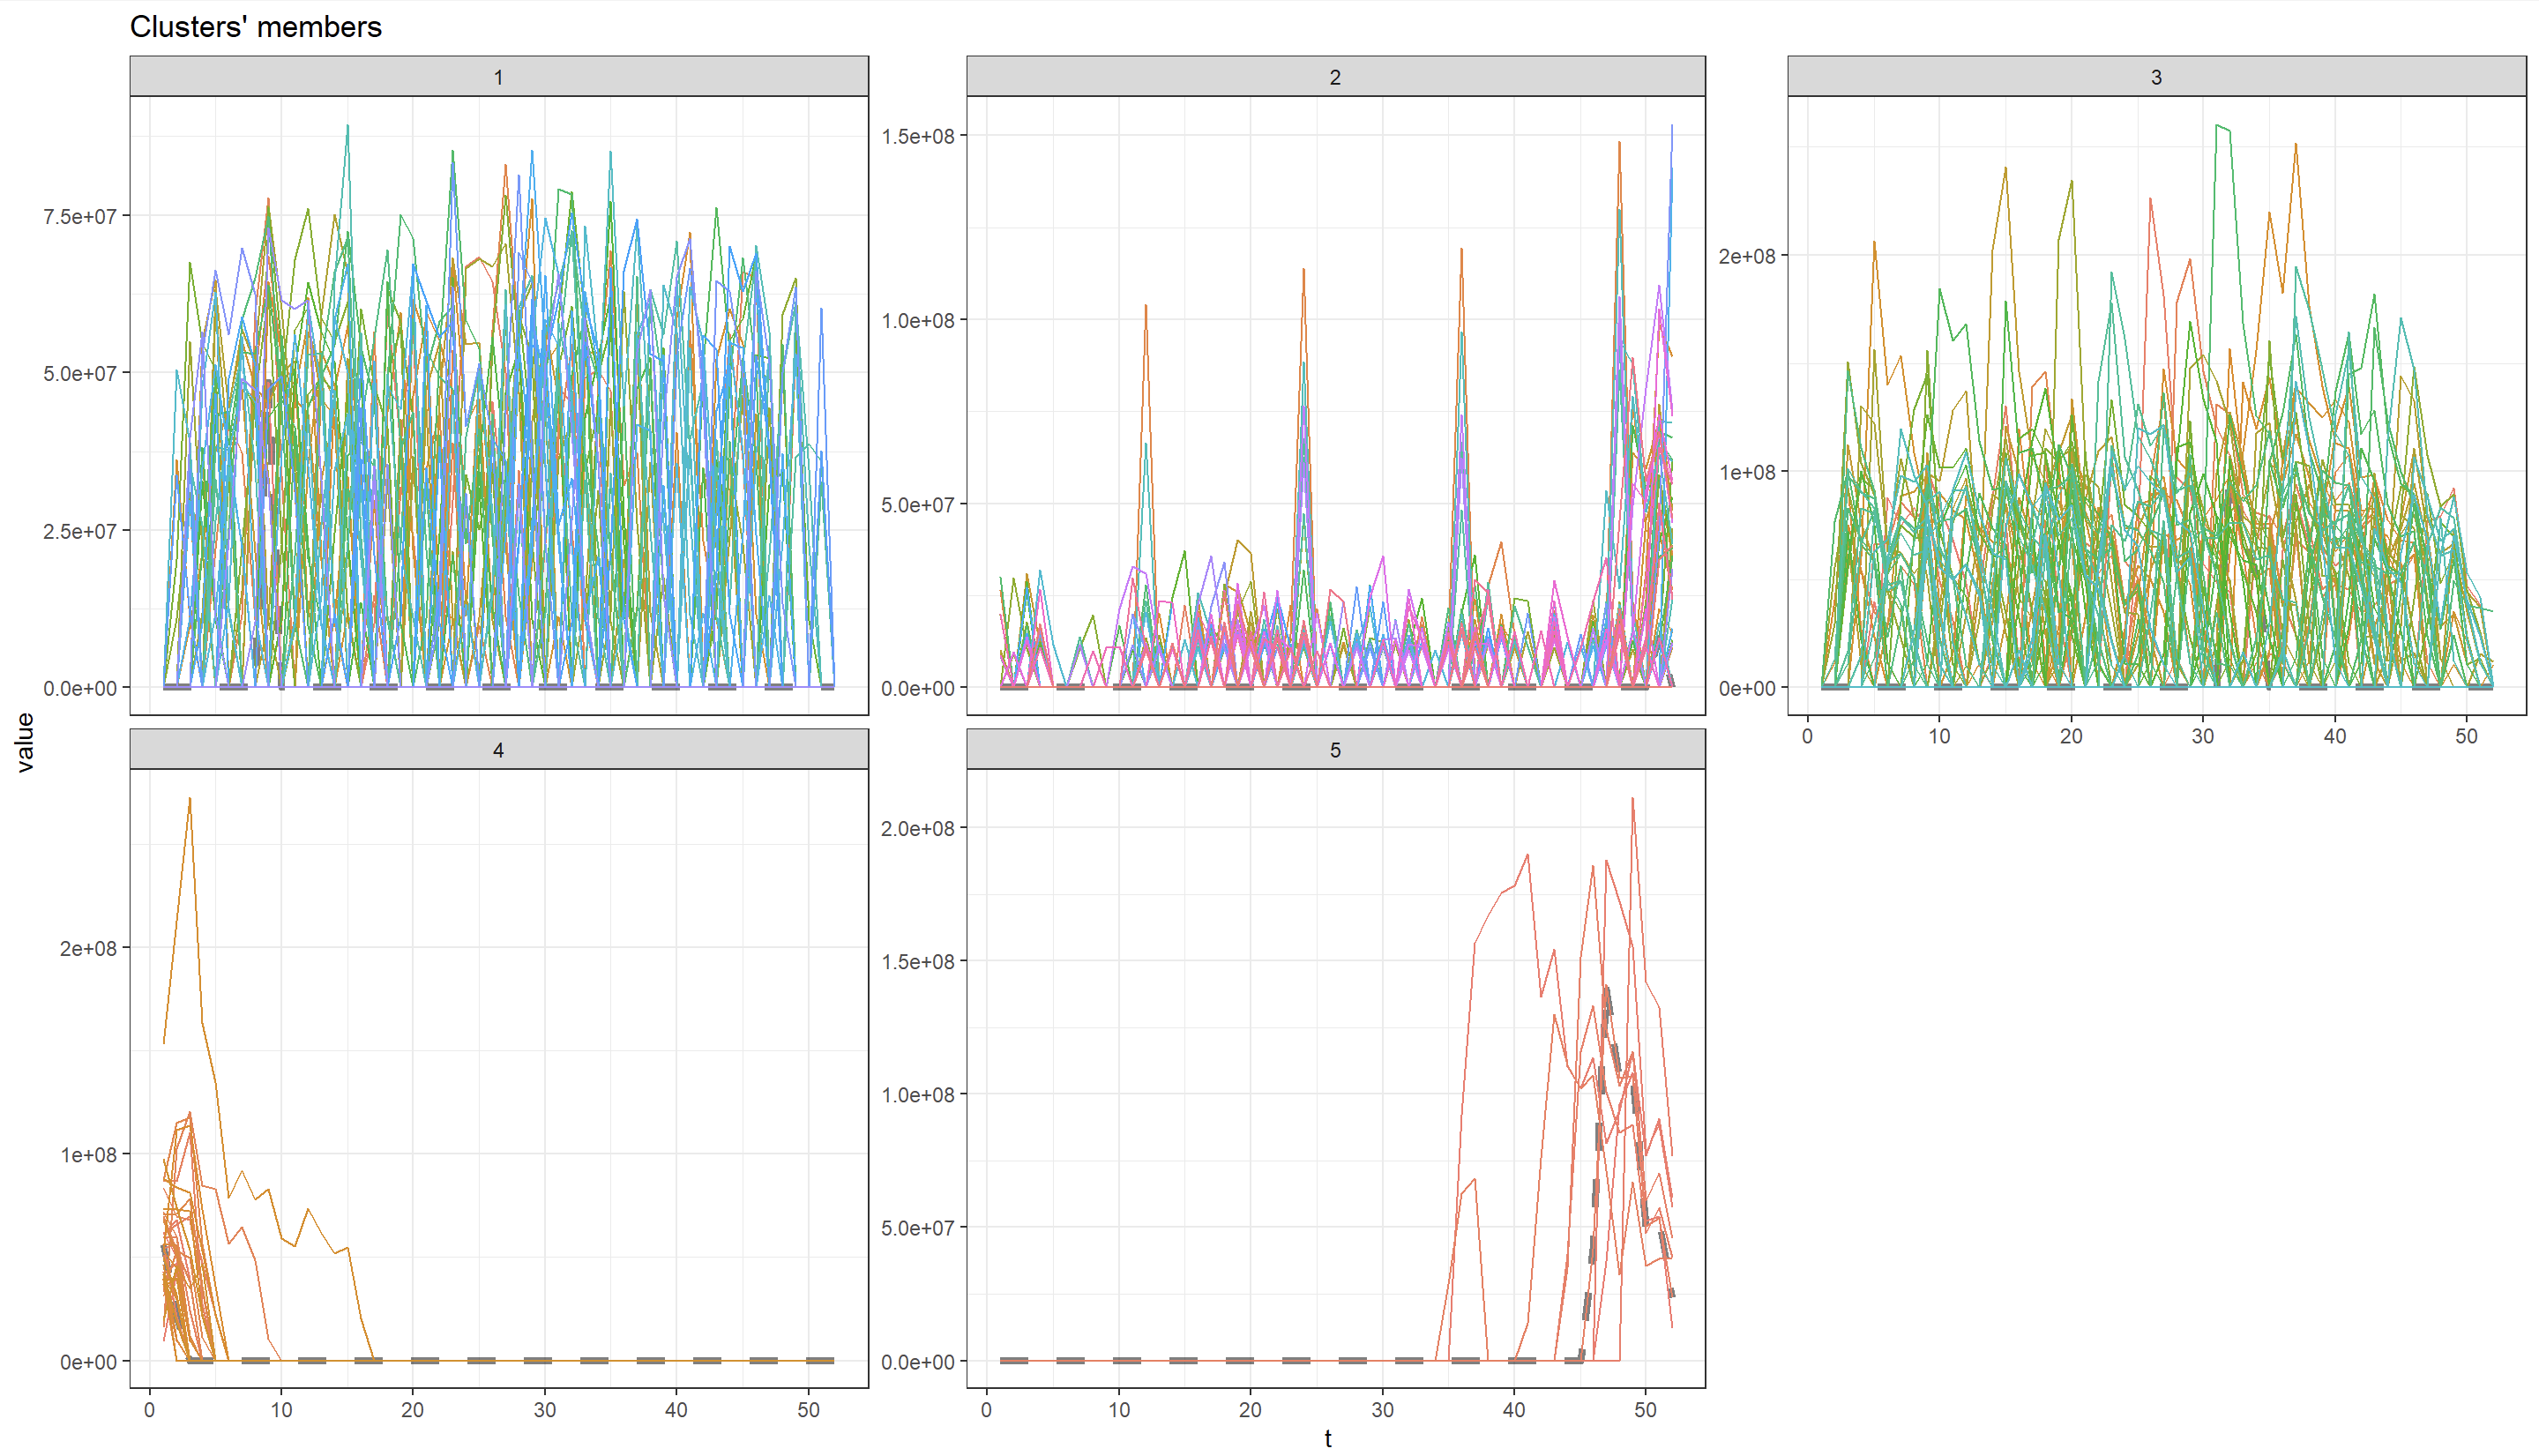
\includegraphics[width=0.8\textwidth]{Images/4_clustering/time_series/tsclust_sc.png}
    \caption{Gràfics de \textit{tsclust} amb l'evolució de streams per cada clúster}
    \label{fig:TS_tsclust_sc}
\end{figure}


Per poder acabar de visualitzar millor les conclusions anteriors s'ha creat un \textit{plot} per a cada classe representant l'evolució dels streams mensuals per cançó. Com podem veure en la figura \ref{fig:ts_clust_streams_month_cluster}, és molt similar a l'anterior però ens permet entendre millor les distribucions de les sèries. 

Tal i com s'ha mencionat, es pot mencionar que la diferència principal entre els clústers 1 i 3 és que aquests últims són bastant més populars alhora que la variància de streams és major entre cançons. També podem confirmar els forts pics espontanis del grup 2 i la major durada i gran popularitat de l'últim clúster (el 5).

A més, es pot veure com el clúster 3 (que conté les cançons que són generalment més populars) té una falta de cançons a l'inici i al final de la línia temporal. Això sembla justificar que el clúster 4 (amb nivells de popularitat semblants al grup 3) és el que conté les primeres cançons que haurien d'anar al clúster 3 (segurament separades pel fet de que han estat ``tallades'' per l'inici de la línia temporal, de manera que la seva sèrie temporal té una forma diferent); mentre que les cançons del clúster 5 semblen ser les cançons populars que haurien de correspondre al clúster 3, i les menys populars semblen haver anat al clúster 2 (degut a l'increment de reproduccions en aquest clúster al final de la seva línia temporal).

\begin{figure}[H]
    \centering
    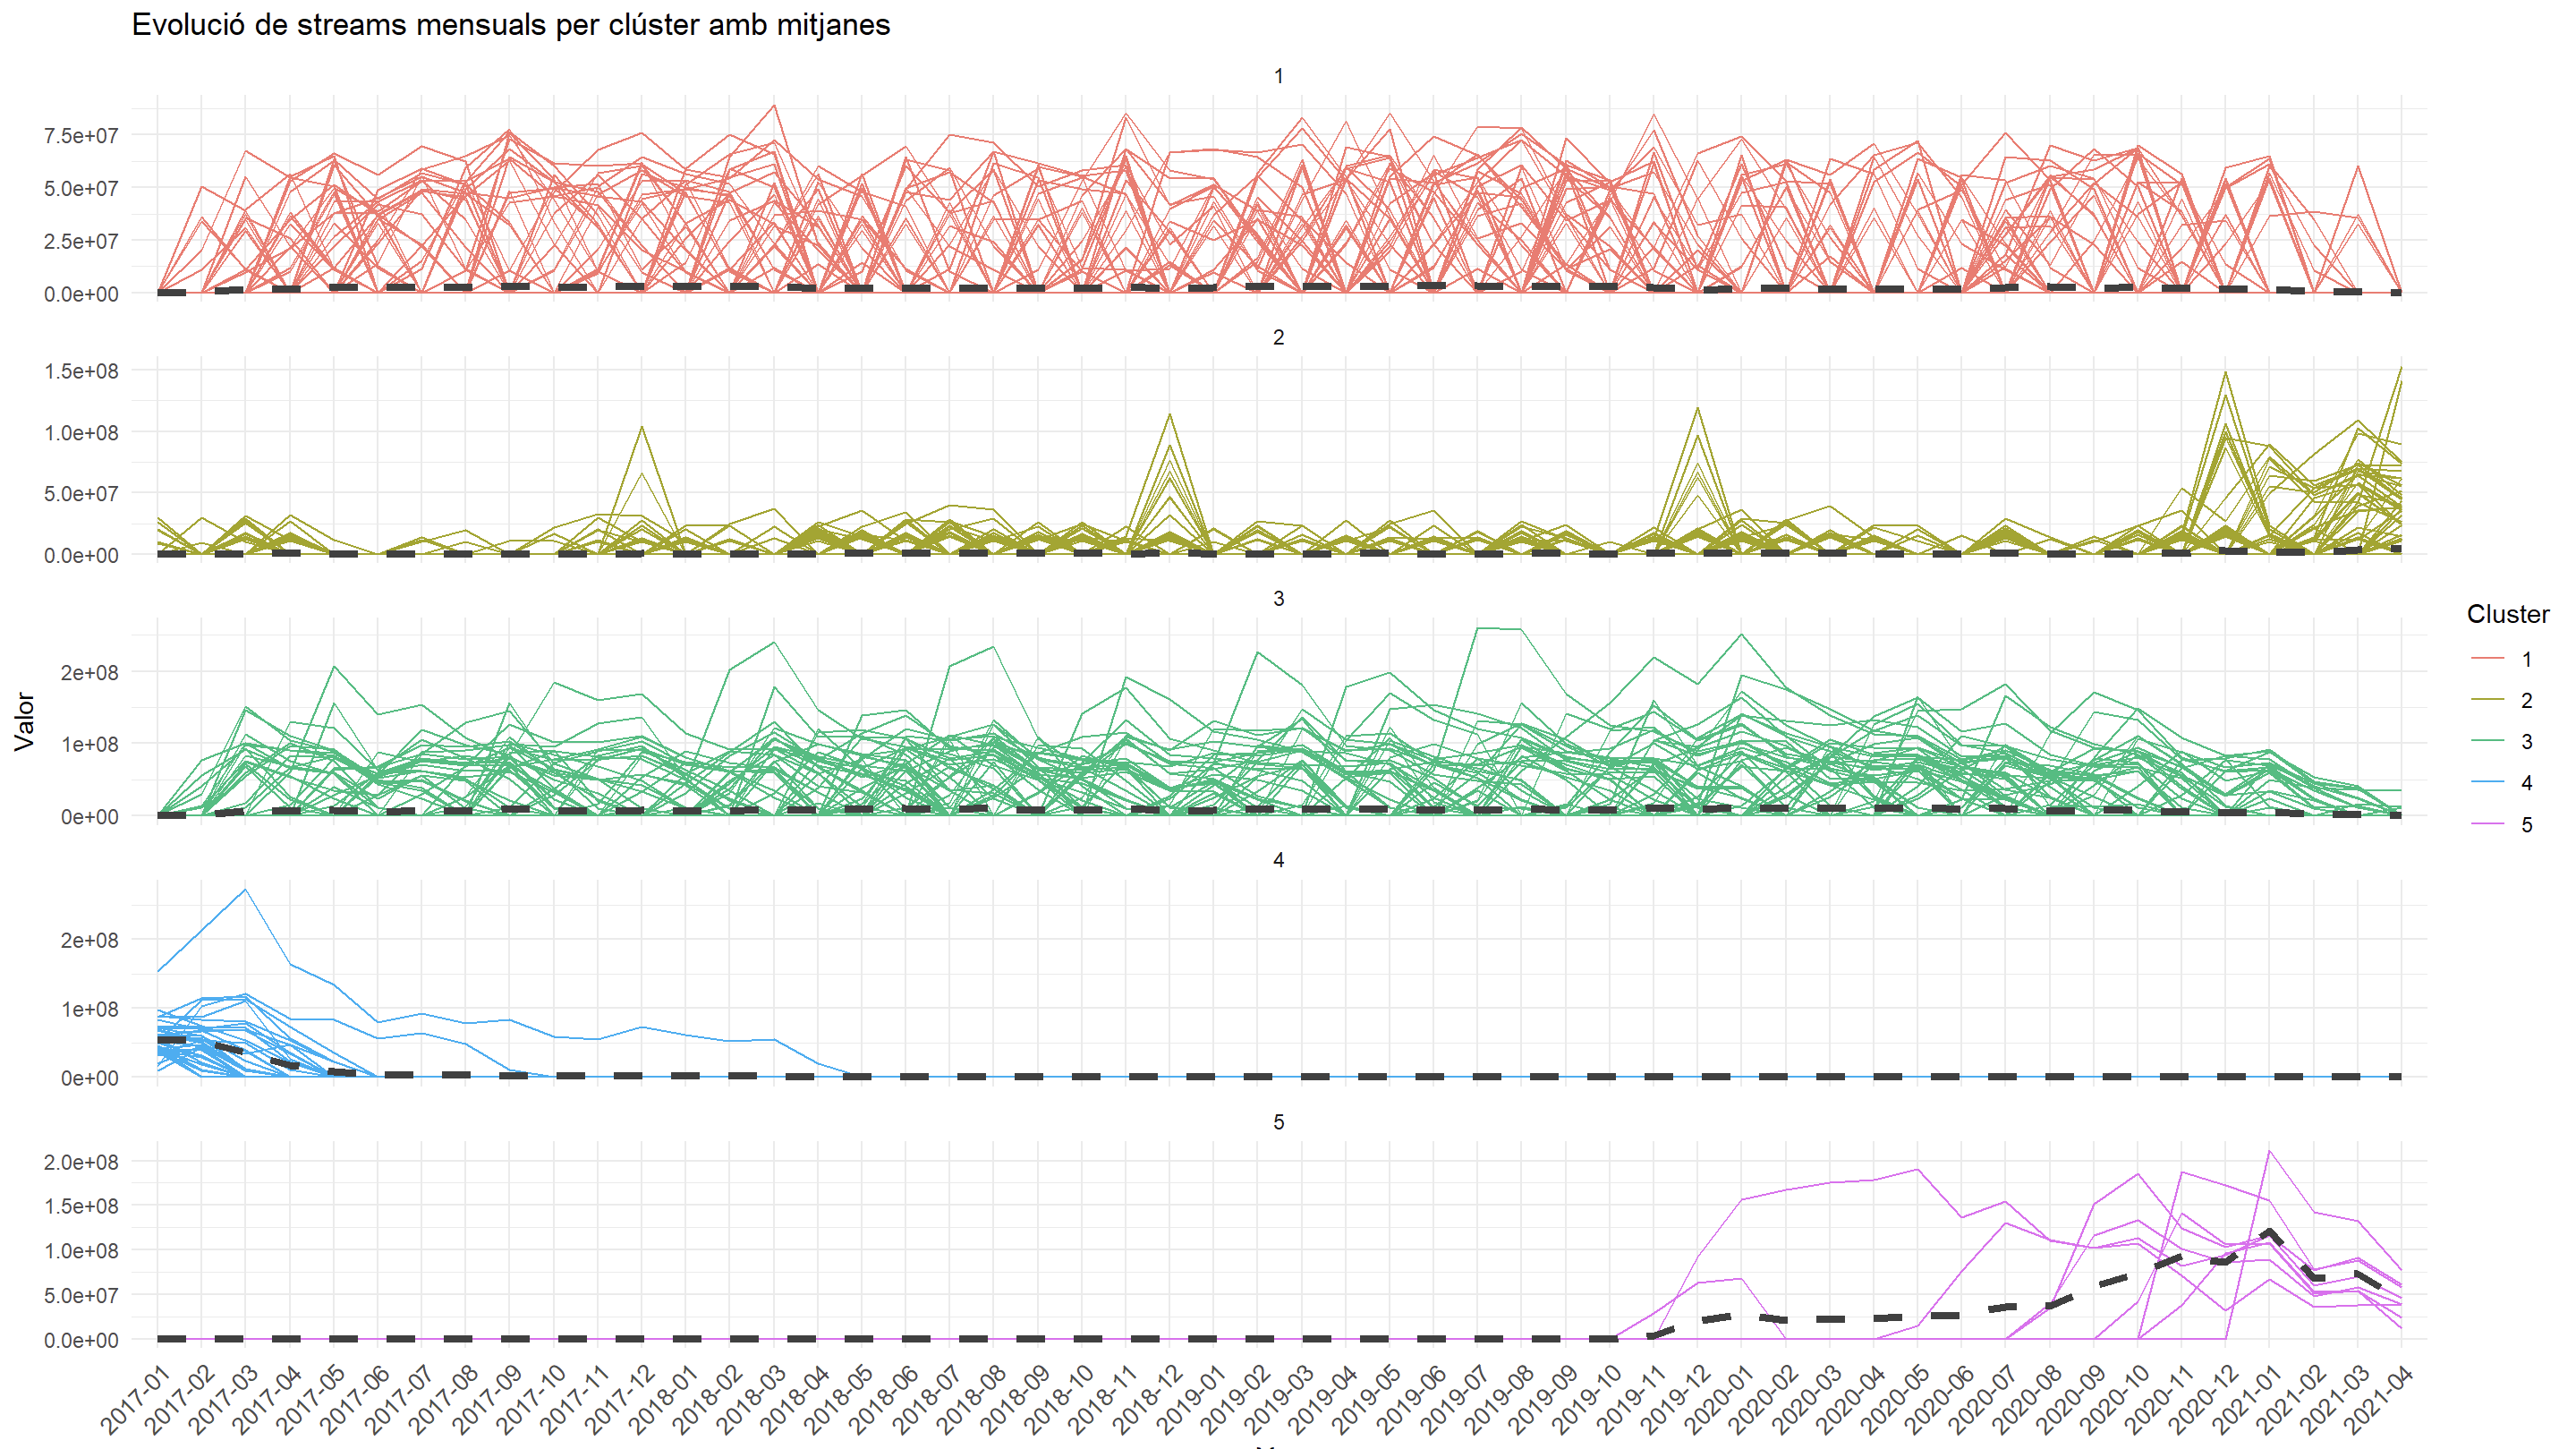
\includegraphics[width=0.8\textwidth]{Images/4_clustering/time_series/streams_cada_mes_per_cluster_amb_mitjana.png}
    \caption{Gràfics de l'evolució de les streams per a cada cançó dins de cada clúster}
    \label{fig:ts_clust_streams_month_cluster}
\end{figure}

Després d'analitzar aquestes sèries s'ha considerat important seguir l'estudi observant la mitjana de mesos actius de les cançons de cada grup indicant-nos així quins clústers contenen els èxits més prolongats i confirmant les conclusions anteriors.

En el primer \textit{barplot} \ref{fig:TS_barplot_mitjanes_mesos_actius} mostra la mitjana de mesos actius per clúster on es pot observar que el clúster 5, que és el més petit, conté les cançons que mantenen la popularitat constant durant el període de temps més llarg. El segon clúster que compleix això és el 3, com ja s'havia observat en l'anàlisi previ. 

Si ens fixem en el \textit{boxplot} \ref{fig:TS_boxplot_mesos_actius} podem observar i confirmar l'espontaneïtat de la classe 2 on pràcticament totes les cançons duren un sol mes en el top, encara s'hi poden observar \textit{outliers}.

\begin{figure}[H]
    \centering
    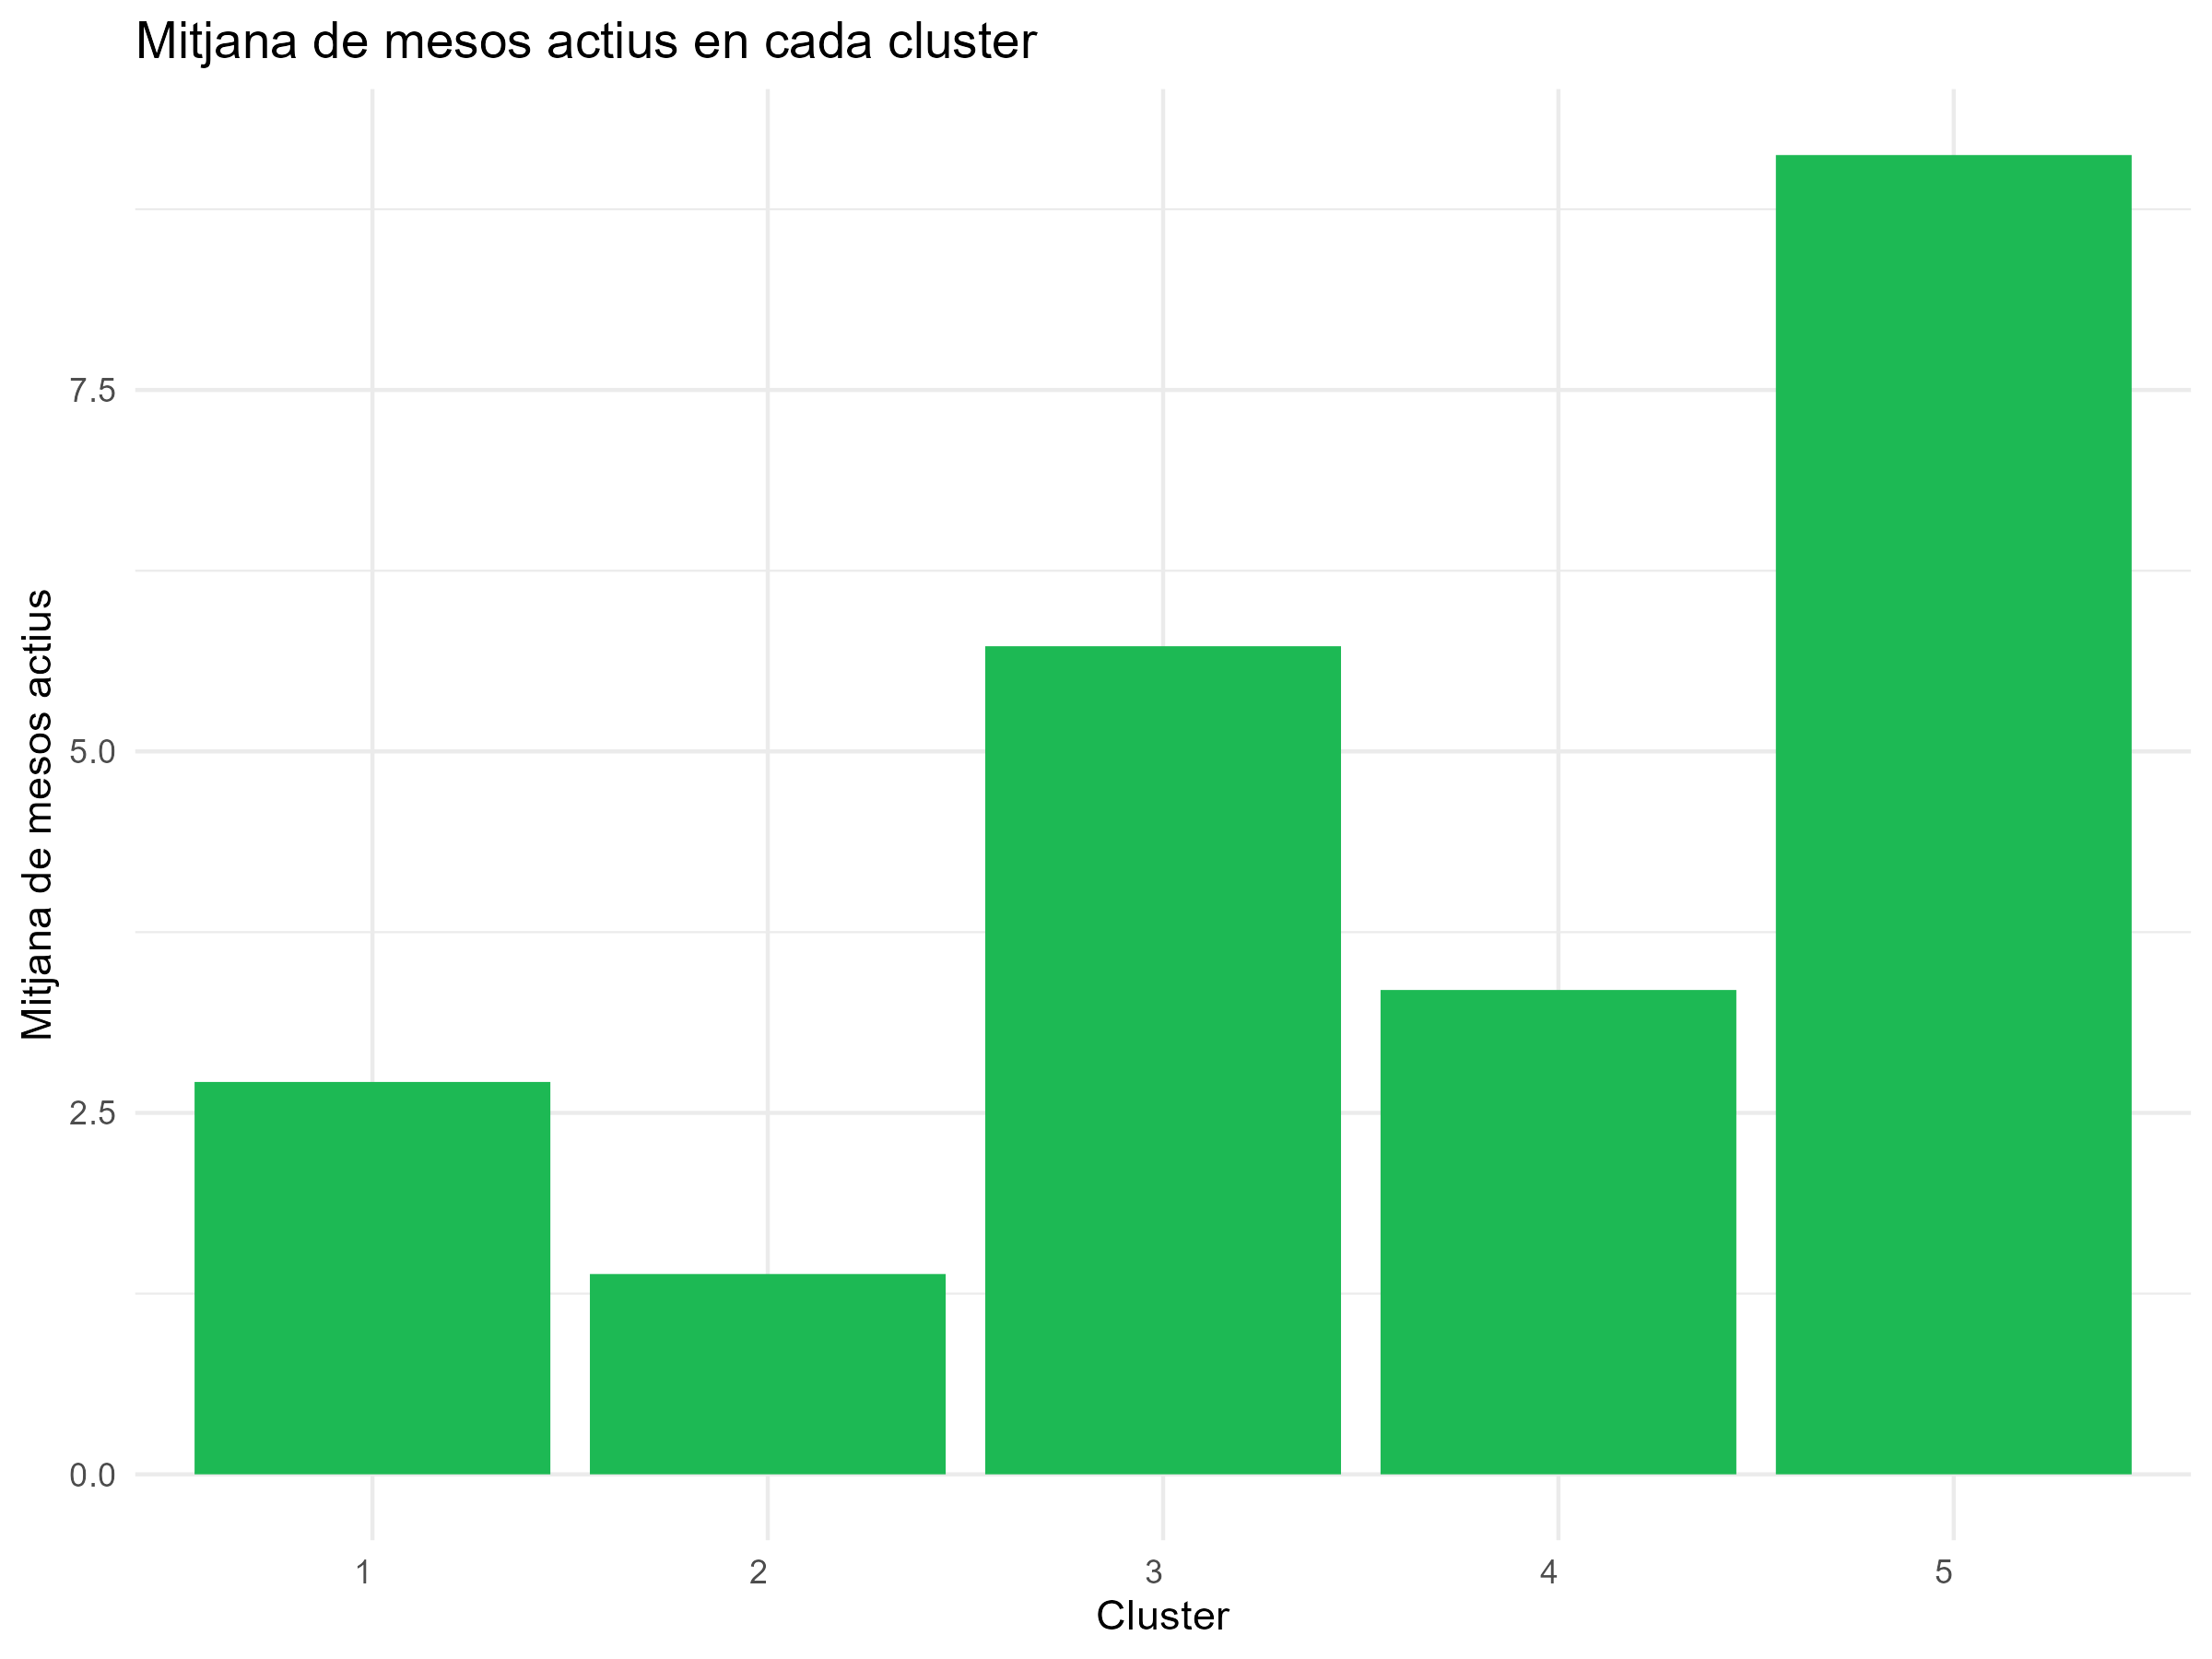
\includegraphics[width=0.8\textwidth]{Images/4_clustering/time_series/barplot_mitjanes_mesos_actius.png}
    \caption{Barplot de la mitjana de mesos actius de les cançons per cada clúster}
    \label{fig:TS_barplot_mitjanes_mesos_actius}
\end{figure}

\begin{figure}[H]
    \centering
    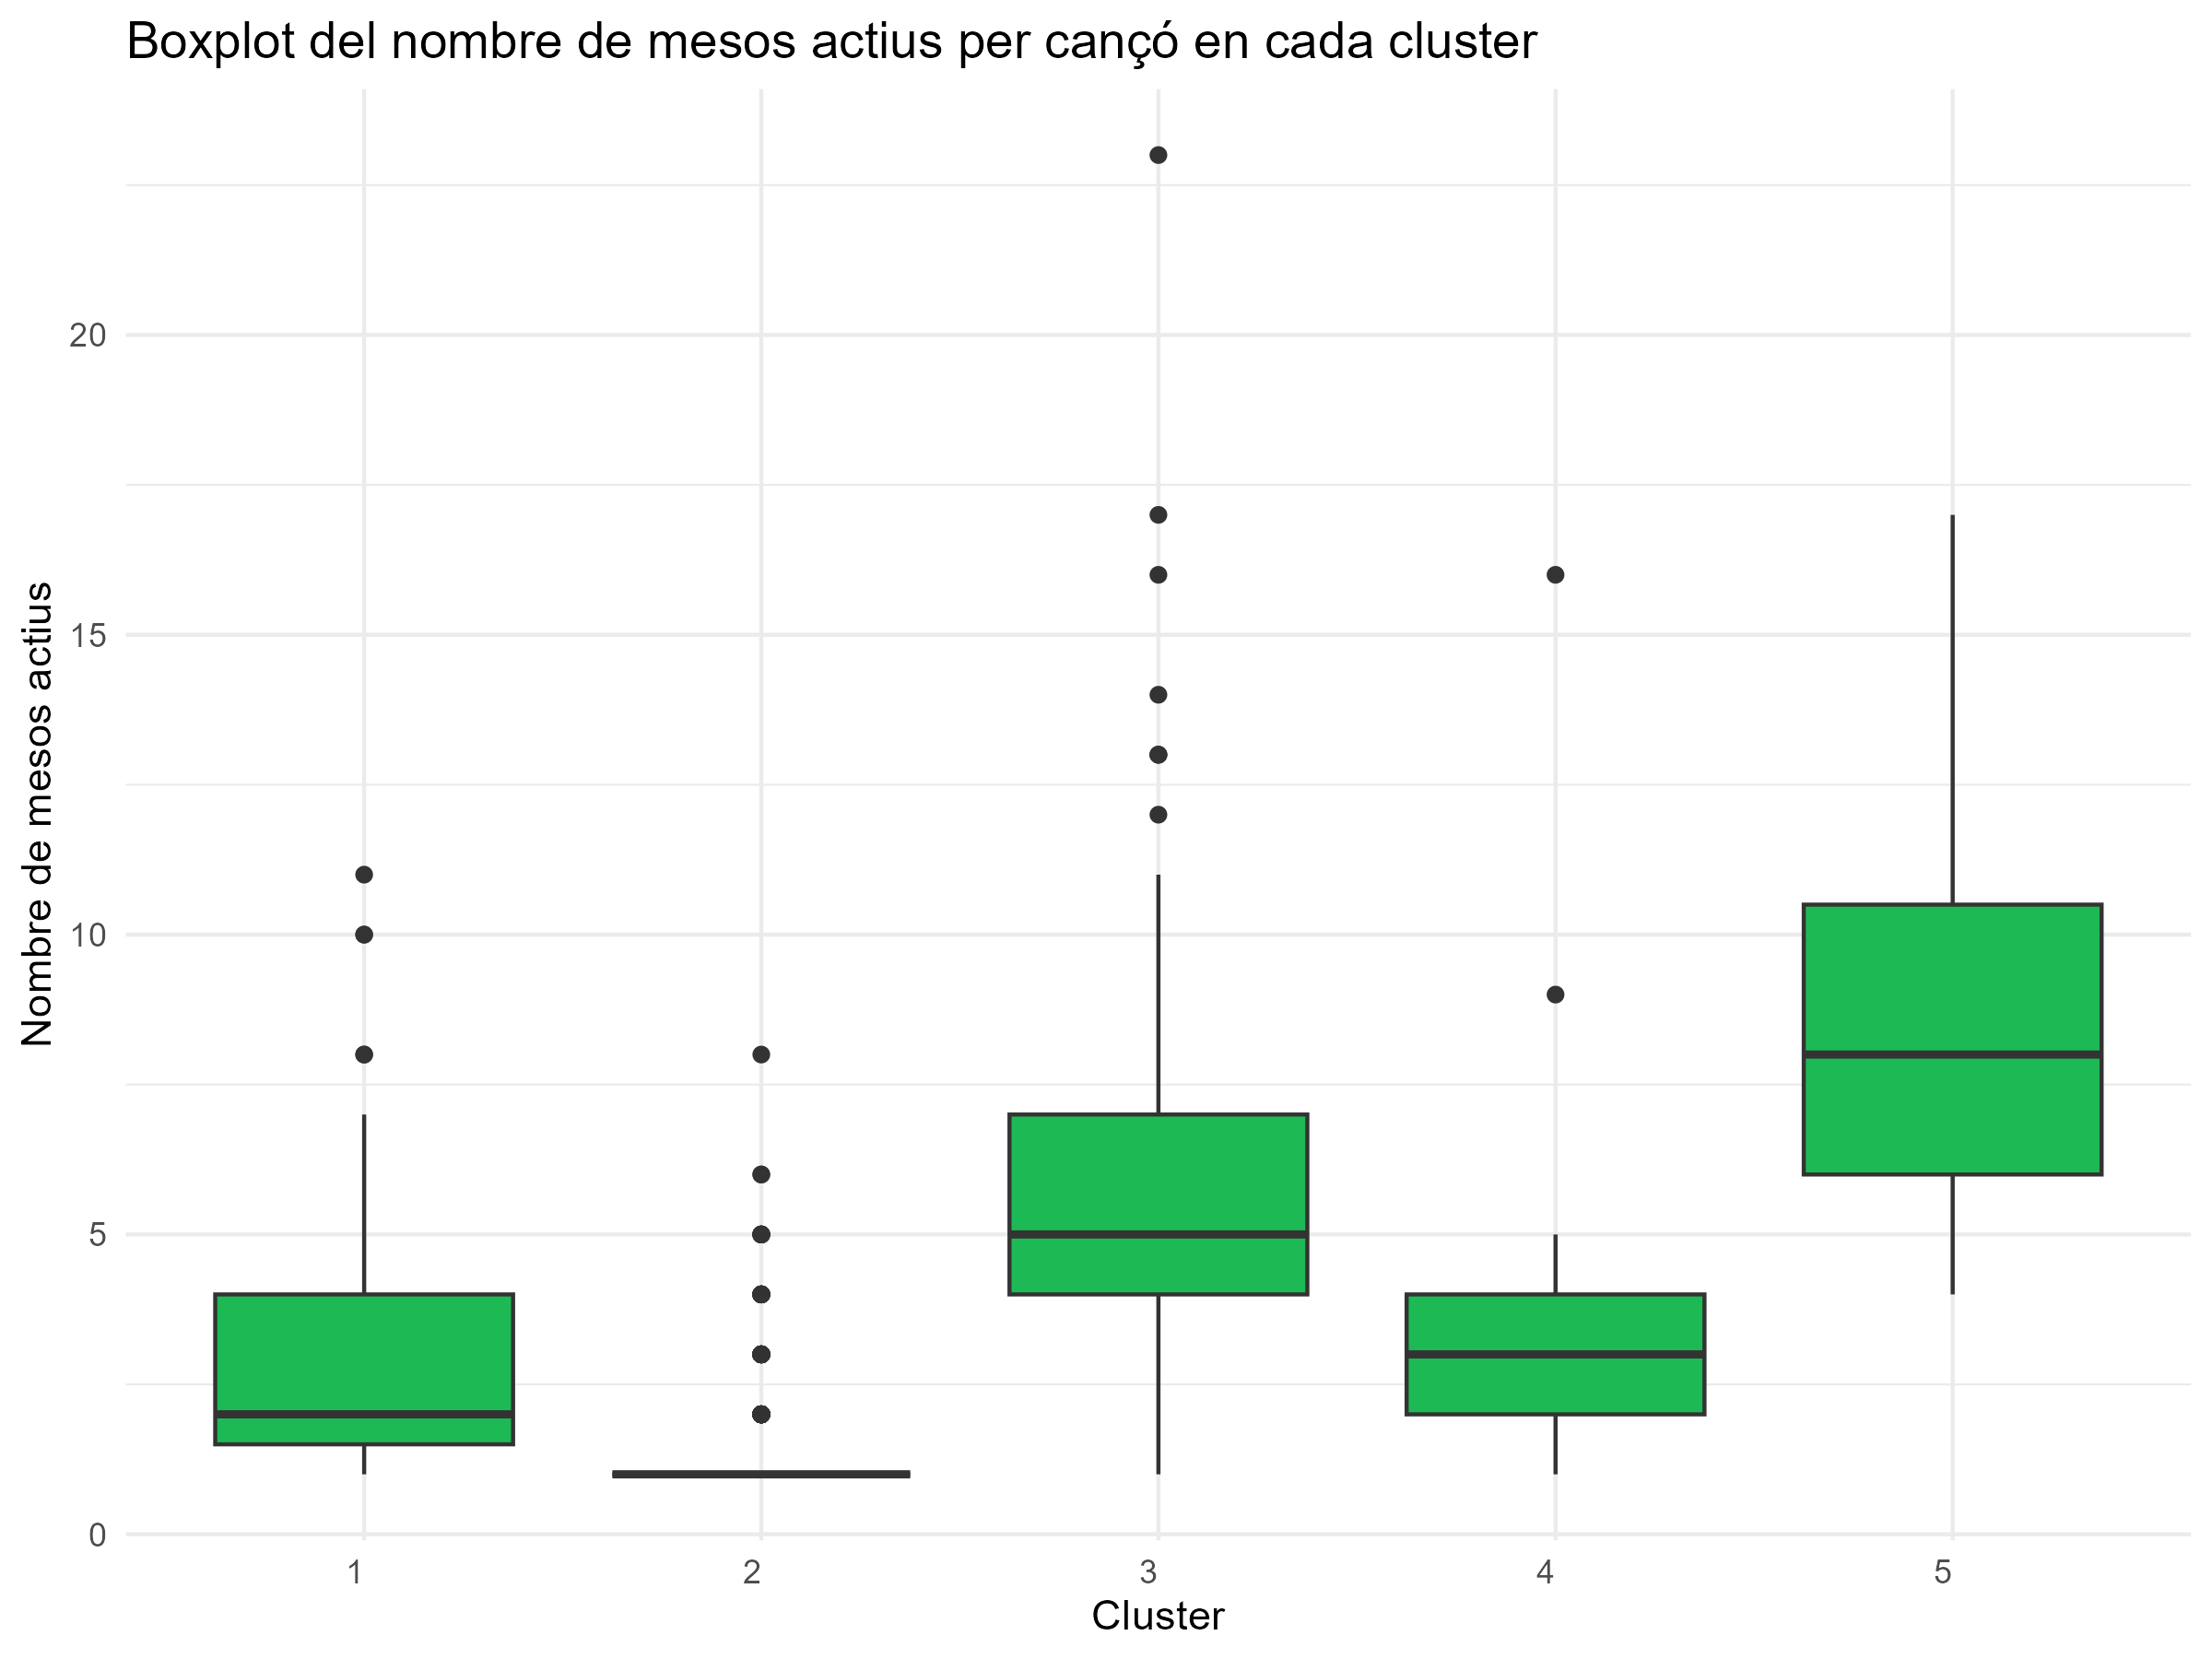
\includegraphics[width=0.8\textwidth]{Images/4_clustering/time_series/boxplot_mesos_actius.png}
    \caption{Boxplot de la distribució de mesos actius de les cançons per cada clúster}
    \label{fig:TS_boxplot_mesos_actius}
\end{figure}

Per poder comprendre millor els clústers, s'ha realitzat un gràfic agrupat per mesos per poder veure si hi ha algun patró estacional ens els diferents clústers. Com es pot veure en la figura \ref{fig:TS_evol_streams_per_mes_i_cluster}, aparentment en els 3 primers clústers no hi ha gaire diferència entre mesos, tan sols es podria comentar un lleuger augment de reproduccions durant els mesos d'estiu.

Pel que fa als clústers 4 i 5, com ja s'ha mencionat prèviament corresponen a les cançons que inicien i acaben els tops en el dataset. Com que els primers valors es van mesurar al gener de 2017, podem veure que en el clúster número 4 (color blau) durant els primers mesos de l'any té moltes streams però a partir del juny ja pràcticament no en té. Per altra banda, el clúster 5, concentra els seus streams durant els mesos d'hivern, ja que és quan hi ha els últims valors mesurats del dataset.

\begin{figure}[H]
    \centering
    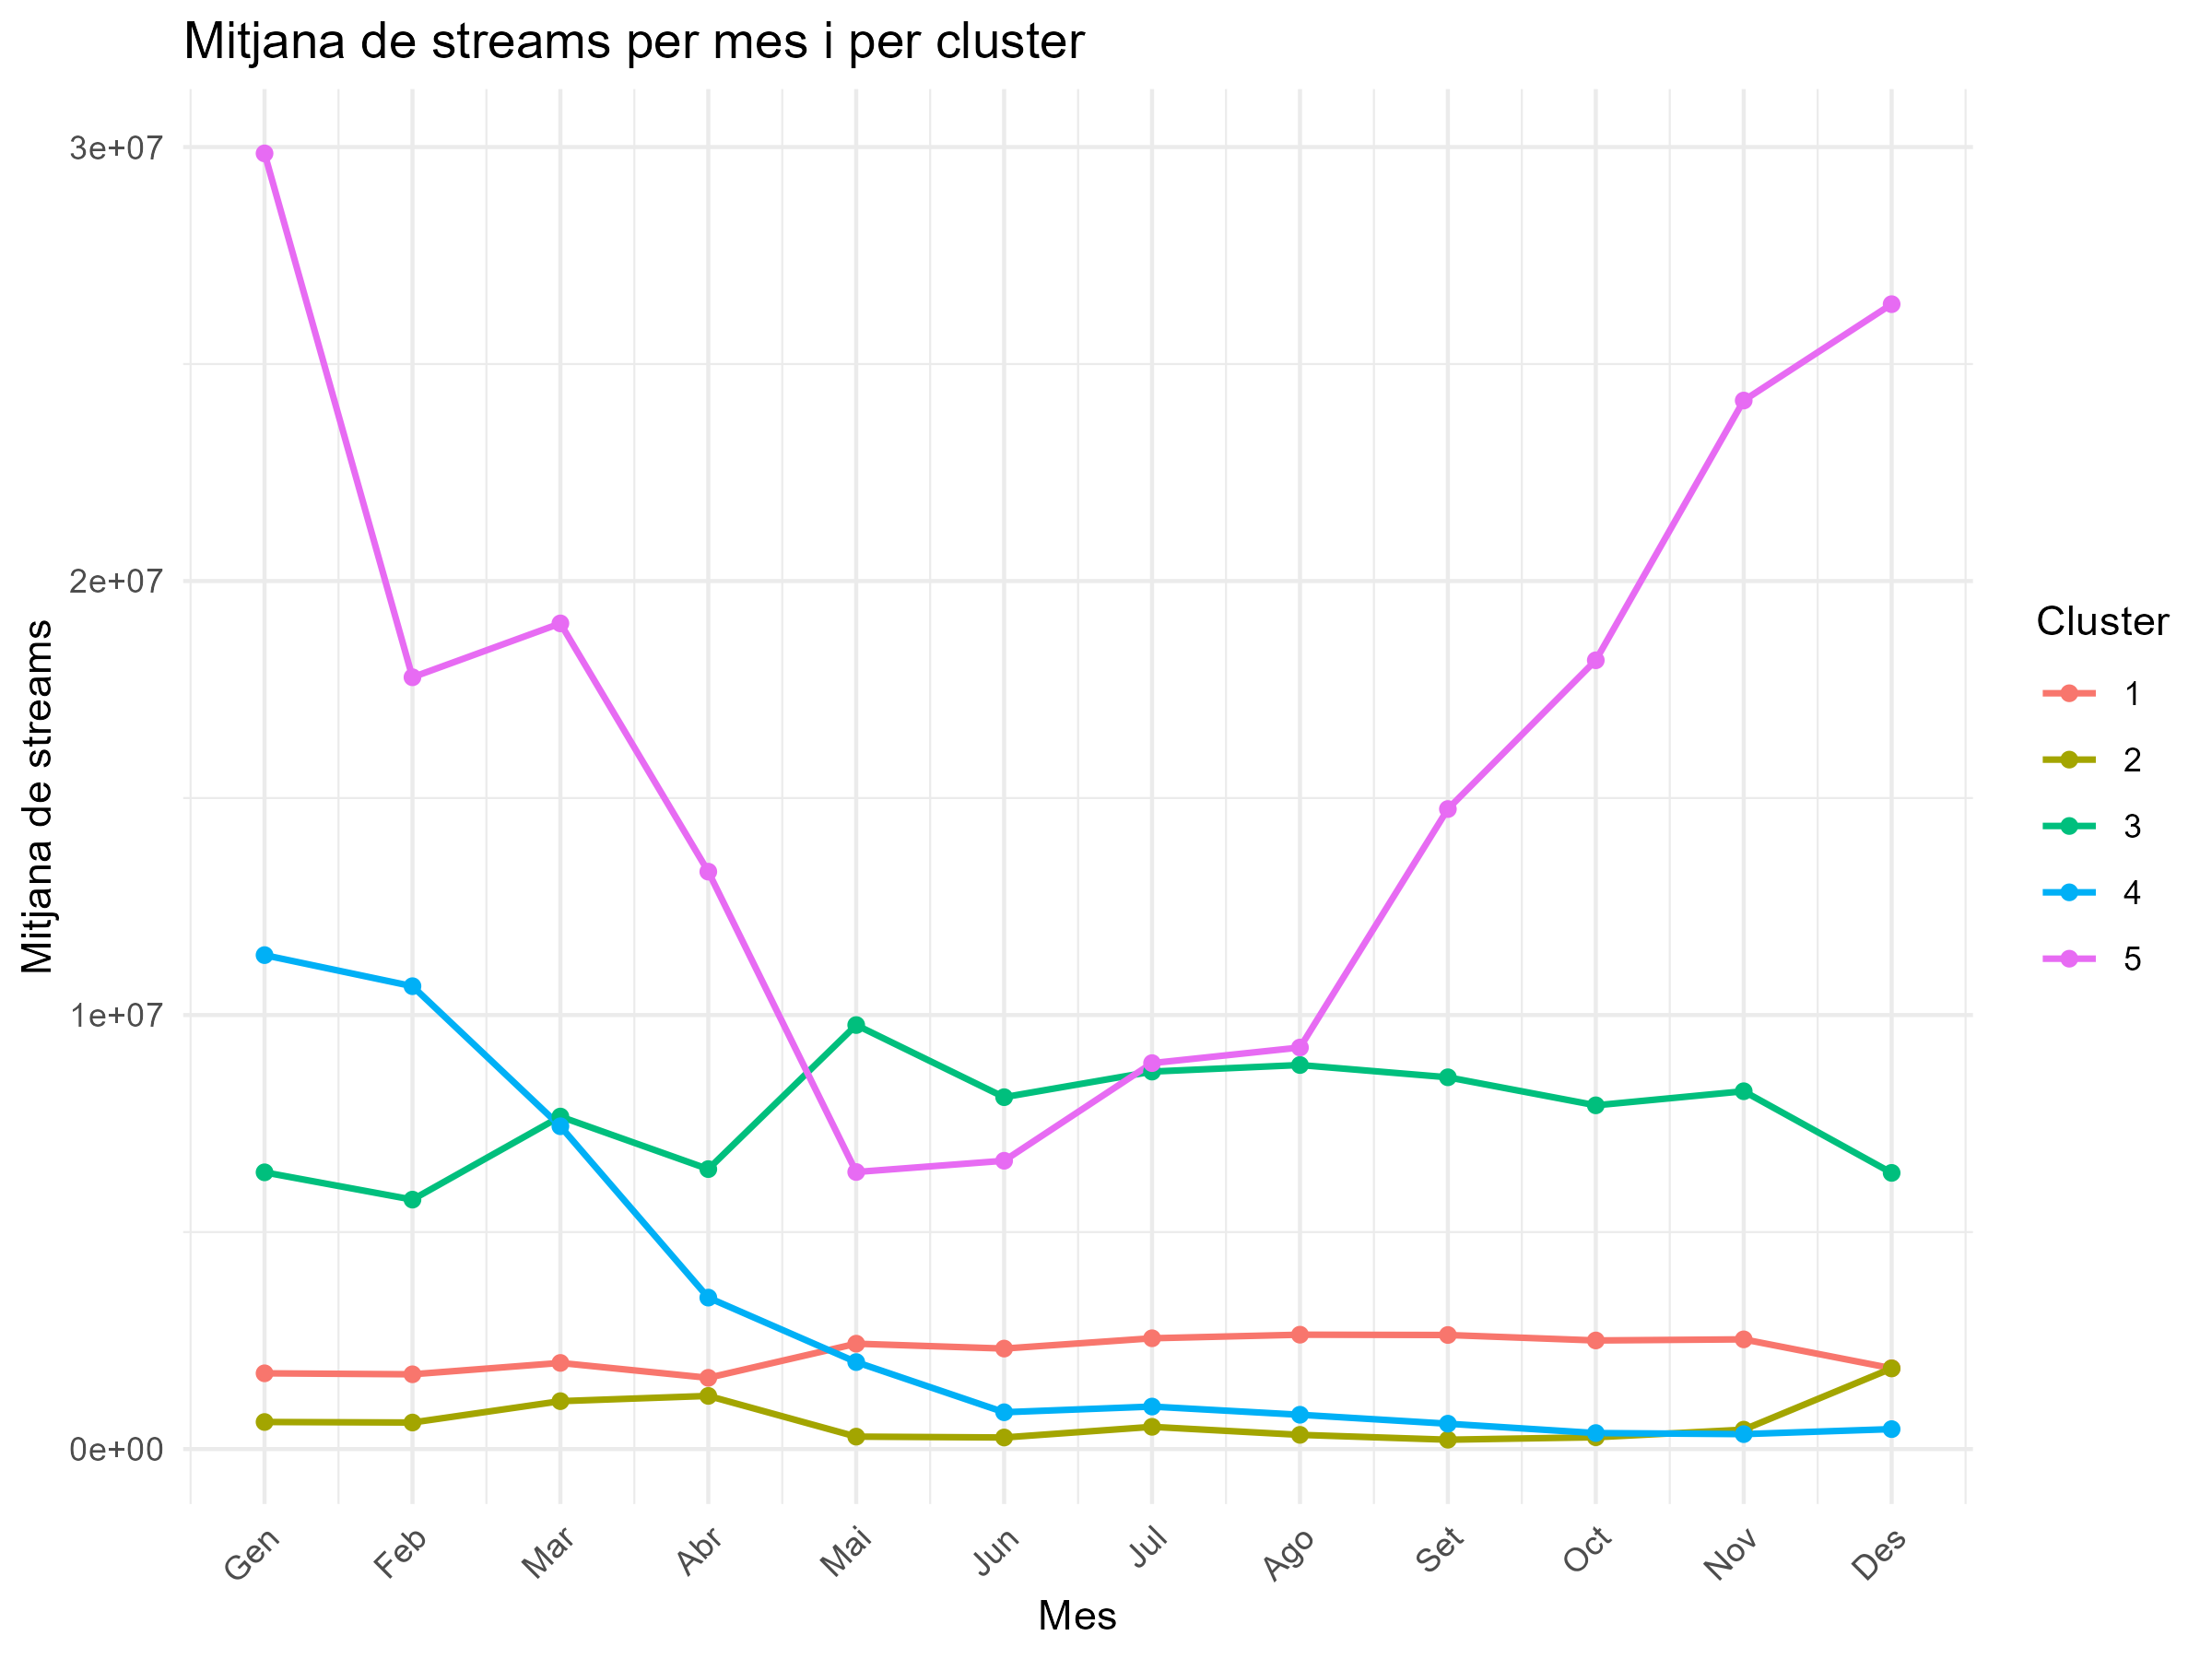
\includegraphics[width=0.8\textwidth]{Images/4_clustering/time_series/evol_streams_per_mes_i_cluster.png}
    \caption{Gràfic amb la mitjana dels streams de cada clúster en funció dels mesos}
    \label{fig:TS_evol_streams_per_mes_i_cluster}
\end{figure}

Com s'ha mencionat prèviament, quan una cançó no apareix en el top 40 durant tot el mes, el seu valor de streams s'ha considerat 0. Això implica que en el gràfic de la figura \ref{fig:TS_evol_streams_per_mes_i_cluster} les mitjanes inclouen molts zeros, de manera que els resultats poden estar condicionats per la quantitat de mesos actius de cada clúster (que ja s'ha vist prèviament). Per tal de veure l'evolució de les mitjanes de streams al llarg dels mesos només tenint en compte quan les cançons estan al top 40 (sense considerar els zeros) s'ha creat el gràfic de la figura \ref{fig:TS_evol_streams_per_mes_i_cluster_no_zeros}. Com es pot veure, el canvi és important, i ara s'aprecia com, per exemple, el clúster 2 té un increment de streams en el mes de desembre (tal i com es veia en els pics mencionats prèviament), però durant tot i així té una mitjana de streams baixa al llarg de tot l'any. Pel que fa al clúster 1, és el més estable de tots i no conté cançons gaire populars. Per altra banda, el clúster 4 té un increment important de streams durant els mesos d'estiu i també al desembre, mantenint en general un nivell mig de popularitat en les seves cançons (tot i que s'ha de tenir en compte que conté cançons només populars al principi del registre, dem manera que en aquest gràfic no s'ha de tenir gaire en compte la seva estacionalitat). Pel que fa al clúster 3, té en general una popularitat alta durant totes les èpoques, sense grans diferències entre elles. Finalment, el clúster oscil·la molt (segurament degut a que només conté 8 cançons) i té una popularitat molt alta en tots els mesos, però especialment durant els primers mesos d'estiu, a la tardor i al gener (tot i que no es pot estudiar gaire la seva estacionalitat degut a que conté cançons només del final del registre).

\begin{figure}[H]
    \centering
    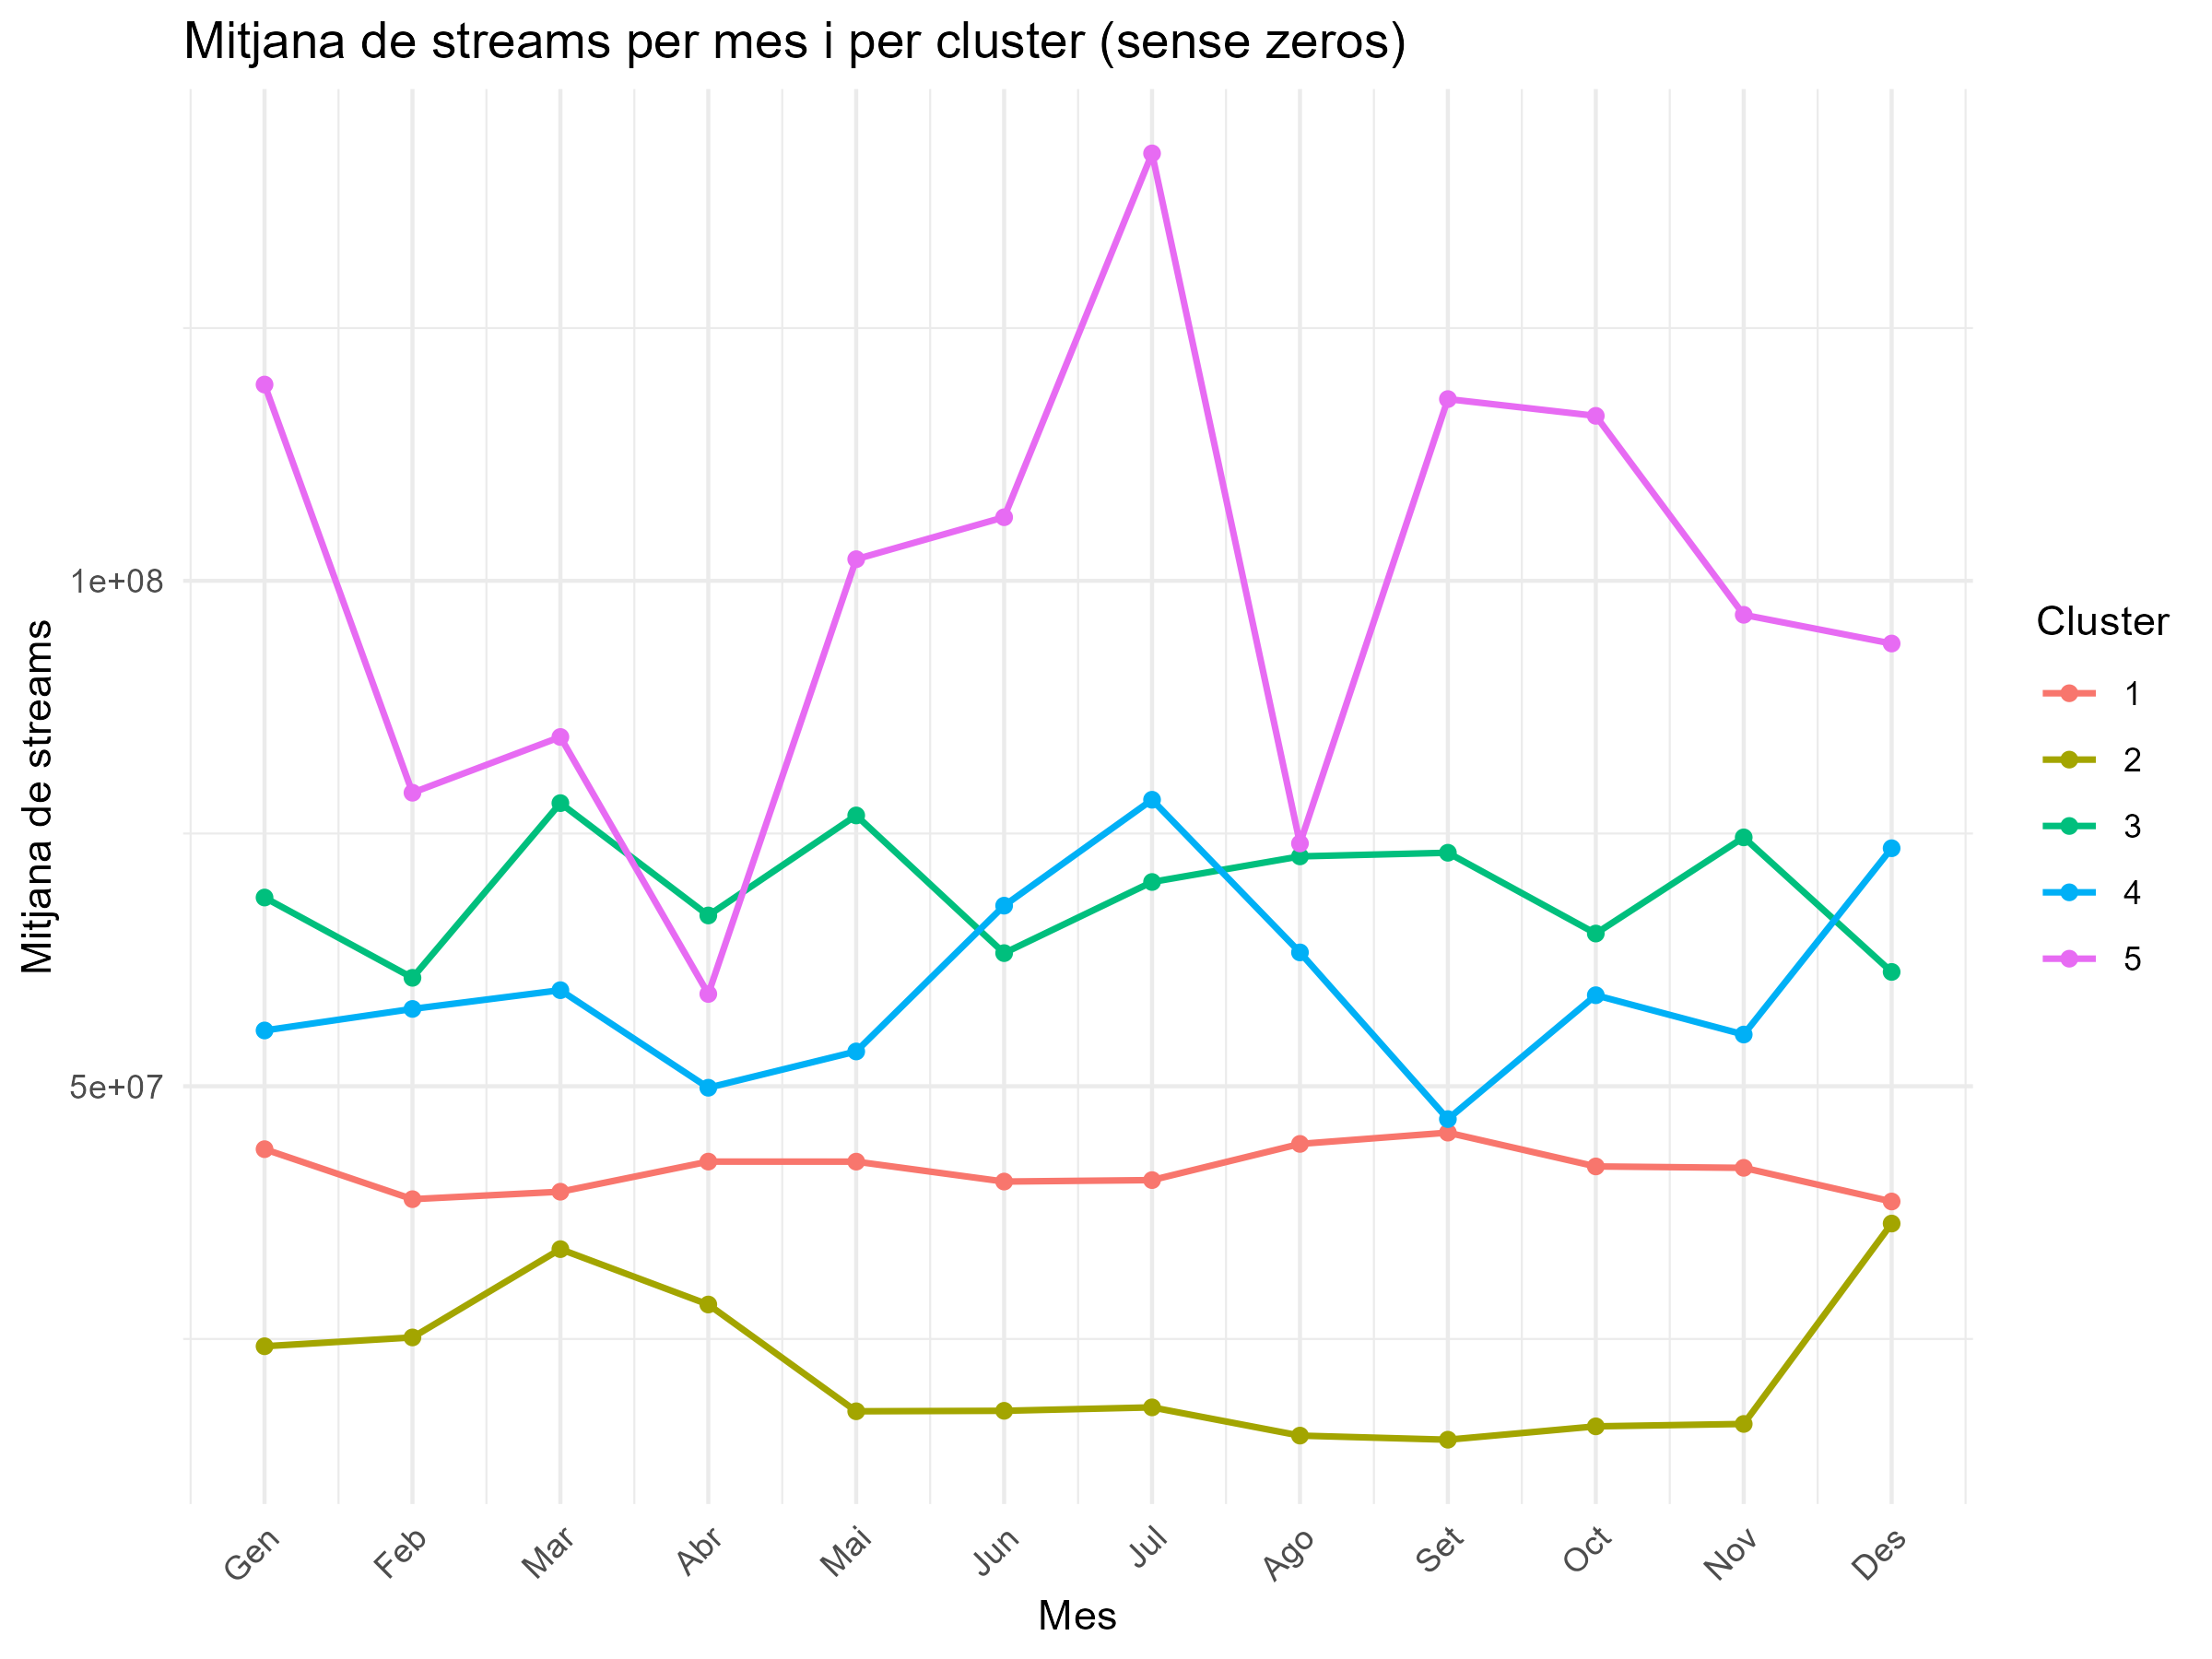
\includegraphics[width=0.8\textwidth]{Images/4_clustering/time_series/evol_streams_per_mes_i_cluster_no_0.png}
    \caption{Gràfic amb l'evolució de la mitjana de streams (sense considerar quan el valor és zero) de cada clúster en funció dels mesos}
    \label{fig:TS_evol_streams_per_mes_i_cluster_no_zeros}
\end{figure}

Amb tot el que s'ha vist, les conclusions són similars a les que s'han mencionat en l'anàlisi inicial. S'ha de tenir en compte que realizar un \textit{profiling} d'aquests clústers no és especialment fàcil, ja que s'han realitzat només tenint en compte el component temporal de streams en la base de dades, ignorant totes les altres variables.

Resumidament, es poden concloure les següents descripcions pels 5 clústers:
\begin{itemize}
    \item \textbf{Clúster 1:} Cançons poc populars i amb una durada no gaire sostinguda al llarg dels mesos.
    
    \item \textbf{Clúster 2:} El grup amb les cançons generalment menys populars i espontànies, tot i que amb alguns hits puntuals al desembre, que s'ha analitzat i, curiosament, no corresponen a cançons de nadal. Sembla contenir les cançons finals no tant populars del clúster 3.
    
    \item \textbf{Clúster 3:} Les cançons generalment més populars, sense ser les més antigues ni les més recents, i bastant sostingudes al llarg dels mesos en el top 40.
    
    \item \textbf{Clúster 4:} Cançons una mica menys populars que en el grup 3 i menys sostingudes, probablement perquè es concentren en els primers anys de la base de dades. Semblen ser les cançons inicials que manquen al clúster 3.
    
    \item \textbf{Clúster 5:} Les cançons més populars, més sostingudes al llarg dels mesos i que encara es trobaven presents al final del registre. Semblen ser les cançons populars finals que manquen al clúster 3.
\end{itemize}

Cal mencionar que l'existència dels clústers 4 i 5 pot ser deguda a que es troben en els inicis/finals dels mesos comptabilitzats a la base de dades, de manera que la seva sèrie temporal probablement té una forma especial (retallada pels extrems) que ha provocat que la distància DTW els separi, resultant en els dos grups amb menys cançons (només 40 i 8).

A més, també es pot afegir que en la figura \ref{fig:TS_dendrograma_colors} es confirma que els clústers 1 i 2 són els més similars, la qual cosa es podia preveure degut a la poca quantitat de streams que comparteixen.


\newpage
\section{Profiling}

Un cop hem utilitzat diferents tècniques de clustering per agrupar les nostres dades, escollint els hiperparàmetres, ara toca fer el profiling. El profiling ens servirà per analitzar els clústers formats durant el clustering jeràrquic i veure com s'han dividit les dades. Per realitzar això, utilitzarem una sèrie de tests d'hipòtesi i gràfiques diverses. També s'intentarà fer una comparació dels clústers que s'han format durant aquest quatrimestre als clústers que van sorgir a ME. Això ens permetrà veure si les noves variables que hem afegit a la base de dades han afectat a l'agrupació o no. 

Primer de tot, trobem interessant veure quantes mostres hi ha a cada un dels clústers. Com veiem a la figura \ref{fig:Cat_BarPlot_cluster_hier}, els 5 clústers escollits no tenen la mateixa mida. Els clústers 1, 2 i 4 tenen mida semblant. No obstant, el tercer clúster té una mida bastant superior als altres i el cinquè clúster no arriba a 1000 instàncies.

\begin{figure}[H] 
    \centering
    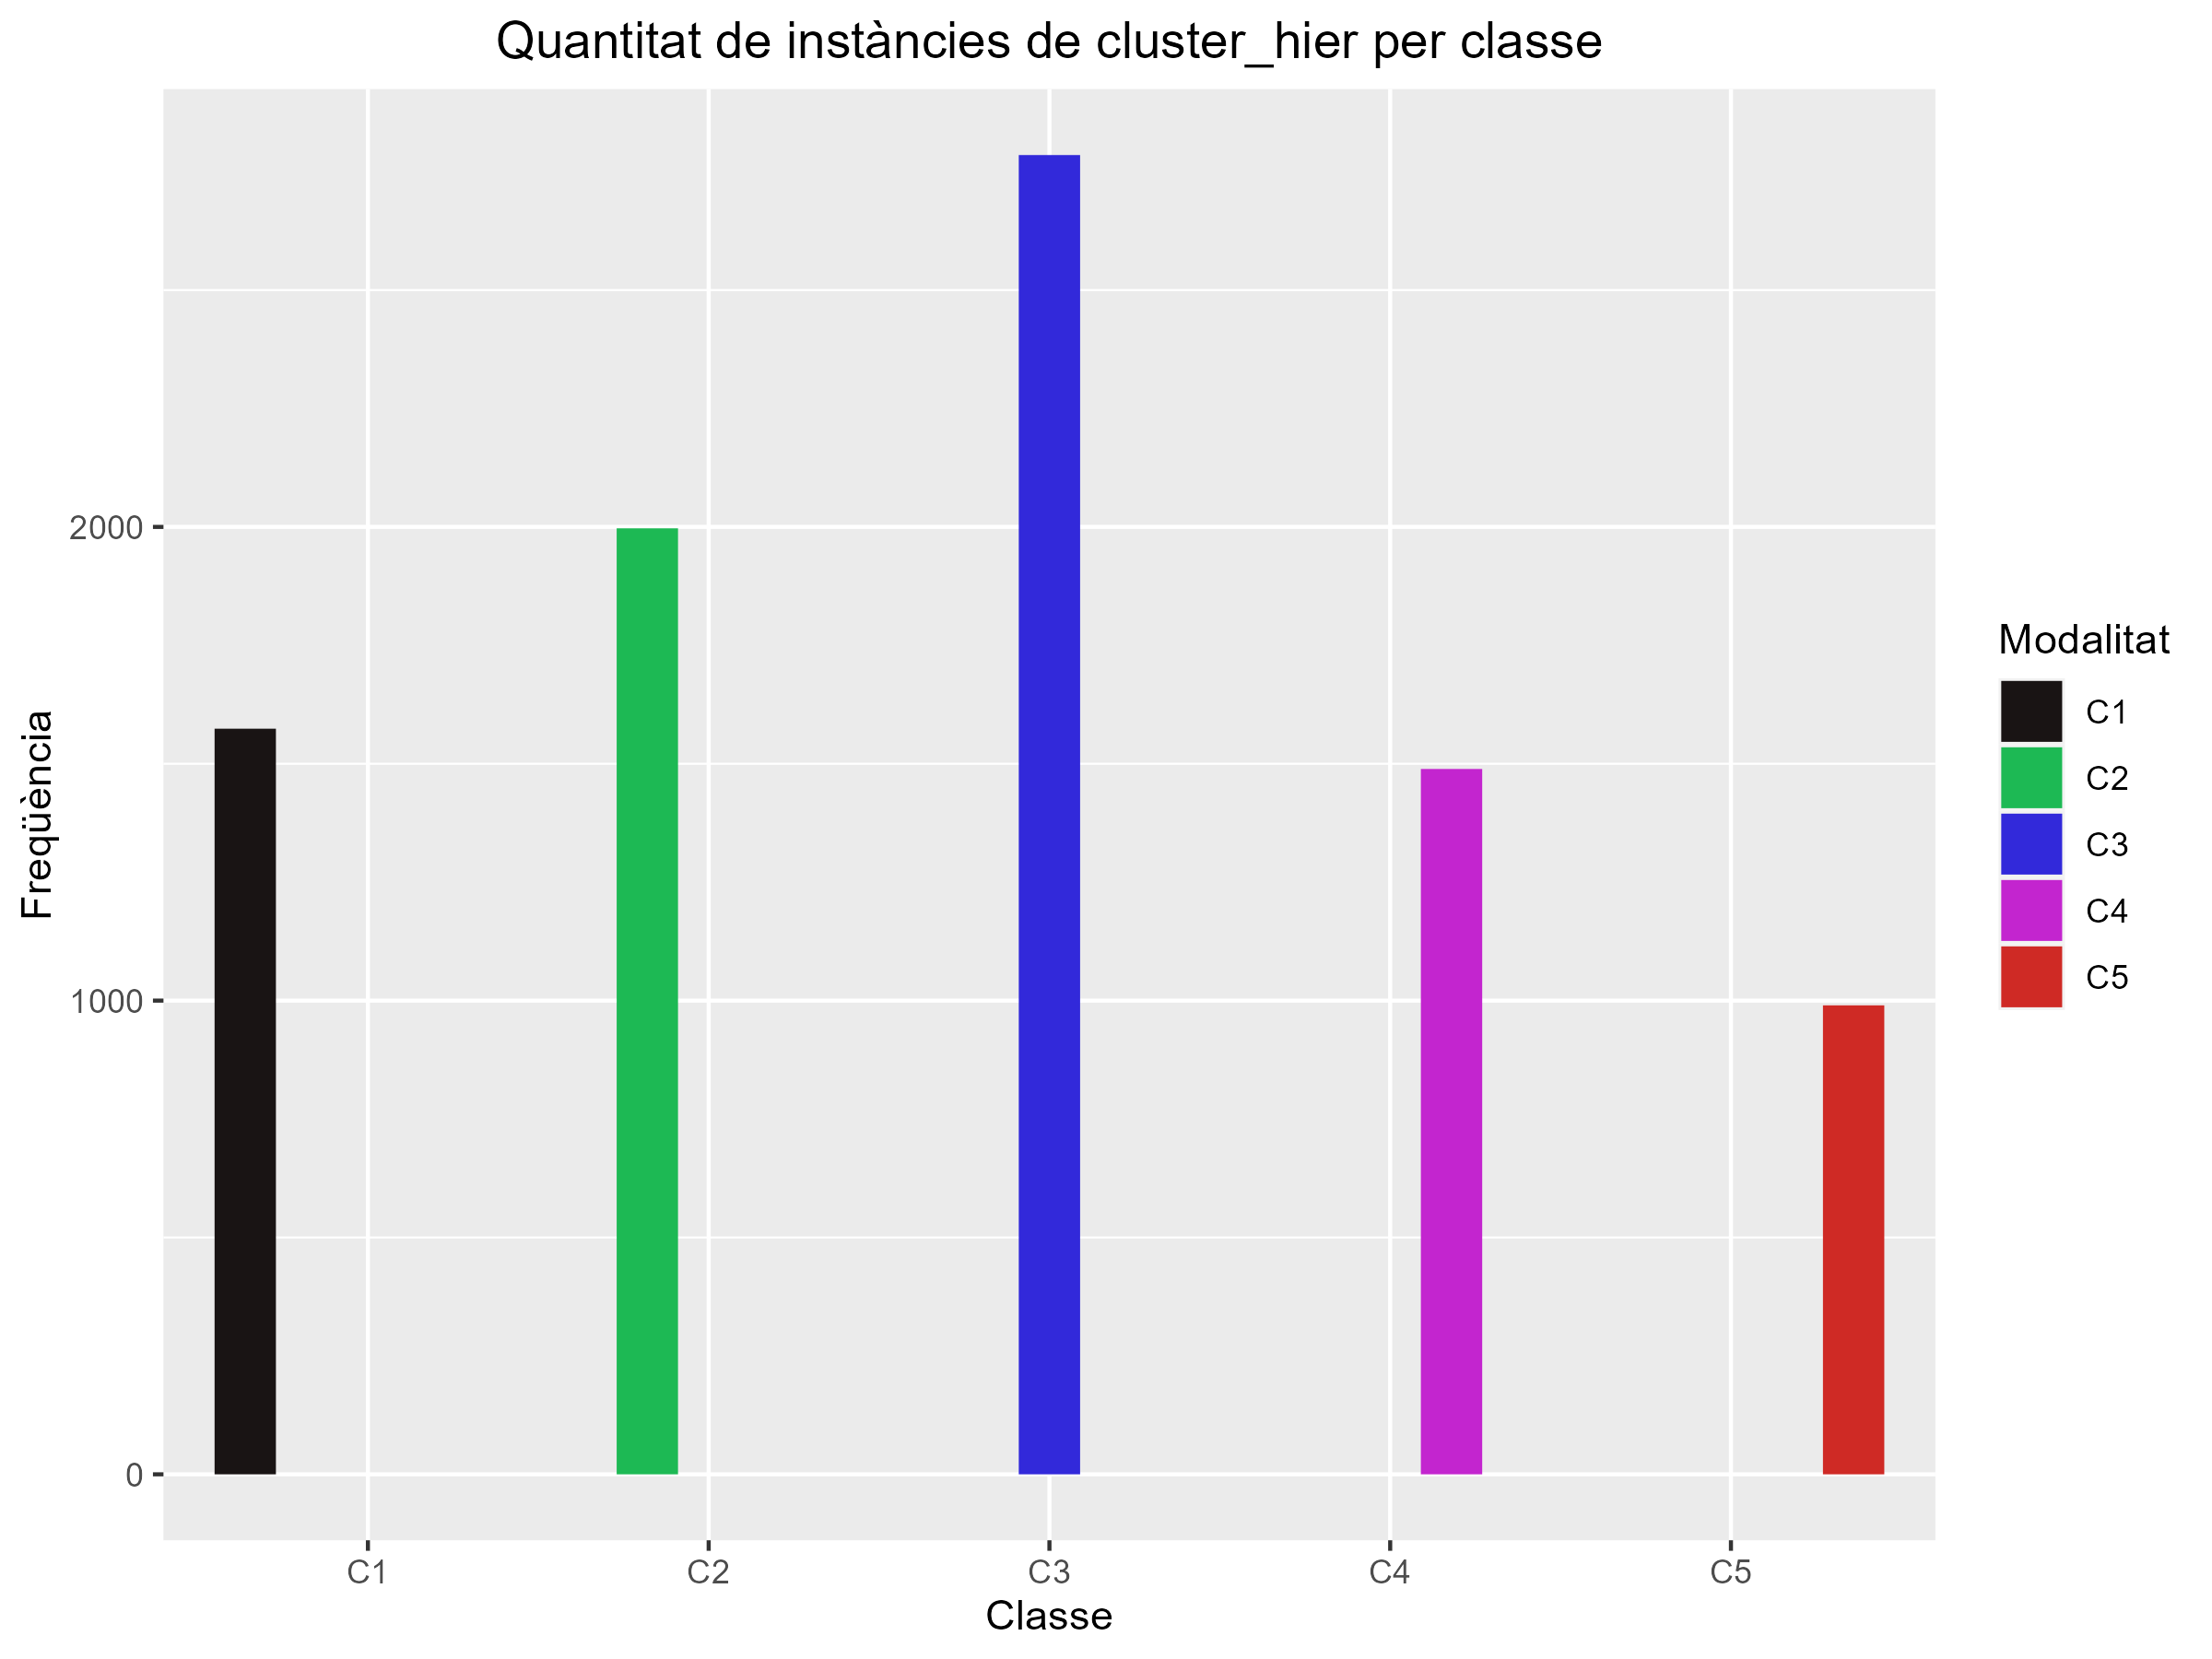
\includegraphics[width=0.7\textwidth]{Images/5_Profiling/categoriques/cat/Cat_BarPlot_cluster_hier.png}
    \caption{Barplot amb la quantitat d'instàncies per clúster}
    \label{fig:Cat_BarPlot_cluster_hier}
\end{figure}

És important, a l'hora de la visualització, tenir en compte que els gràfics de barres estan desbalancejat i que no afecti a la nostra anàlisi. 

\subsection{Variables numèriques}

En el cas de les numèriques, per veure si cada una de les variables és significativa en els clústers, utilitzarem test d'hipòtesi amb els quals ja estem familiaritzats. Farem servir el ANOVA, el Kruskal-Wallis i el t-test i els acompanyarem amb BarPlots i Boxplots per visualitzar les diferències.

El que fa l'ANOVA és comparar les mitjanes de cada variable numèrica en cada un dels clústers, amb això mira si hi ha una diferència significativa entre les mitjanes. La nostra hipòtesi nul·la és que no hi ha diferències significatives entre les mitjanes a cada classe, i la hipòtesi alternativa serà que almenys alguna de les mitjanes de la nostra variable numèrica és diferent depenent de les clases. 

Ja sabem que el test ANOVA assumeix que les nostres variables segueixen una distribució normal, però com el nostre dataset és superior a 100 mostres, segons el teorema del límit central, assumim que la distribució de les nostres variables s'assemblarà a una distribució normal per poder fer aquests tests. Tot i això, per si a cas, també es fa servir un altre test que en aquest cas no requereix que les seves variables sí que tinguin una distribució normal, que és el Kruskal-Wallis. Aquest test té com a objectiu comparar dues mostres, i saber si pertanyen a la mateixa població amb variàncies similars o les segves variàncies són significativament diferents. 

Finalment, també s'ha fet un t-test, que el que fa és comparar les mitjanes de les distribucions que tindrà cada variable dins de cadascun dels clústers amb la mitjana generat que té la variable. Per aquest test la nostra hipòtesi nul·la serà que les mitjanes de la distribució de la variable dins del clústers comparada amb la distribució de la variable total no són significativament diferents. 

Ara sí, podem començar a mirar variable per variable si aporten significativament al clustering format i si ho fan, en quina de les quatre classes està afectant més. En el cas de les numèriques, no s'han afegit noves variables durant el preprocessing, per tant, es faran els tests per les mateixes variables del quatrimestre passat però més tard ja mirarem si es fan coses similars o la formació dels clústers no té res a veure. 

\begin{figure}[H]
\centering
    \begin{minipage}{.49\textwidth}
        \centering
        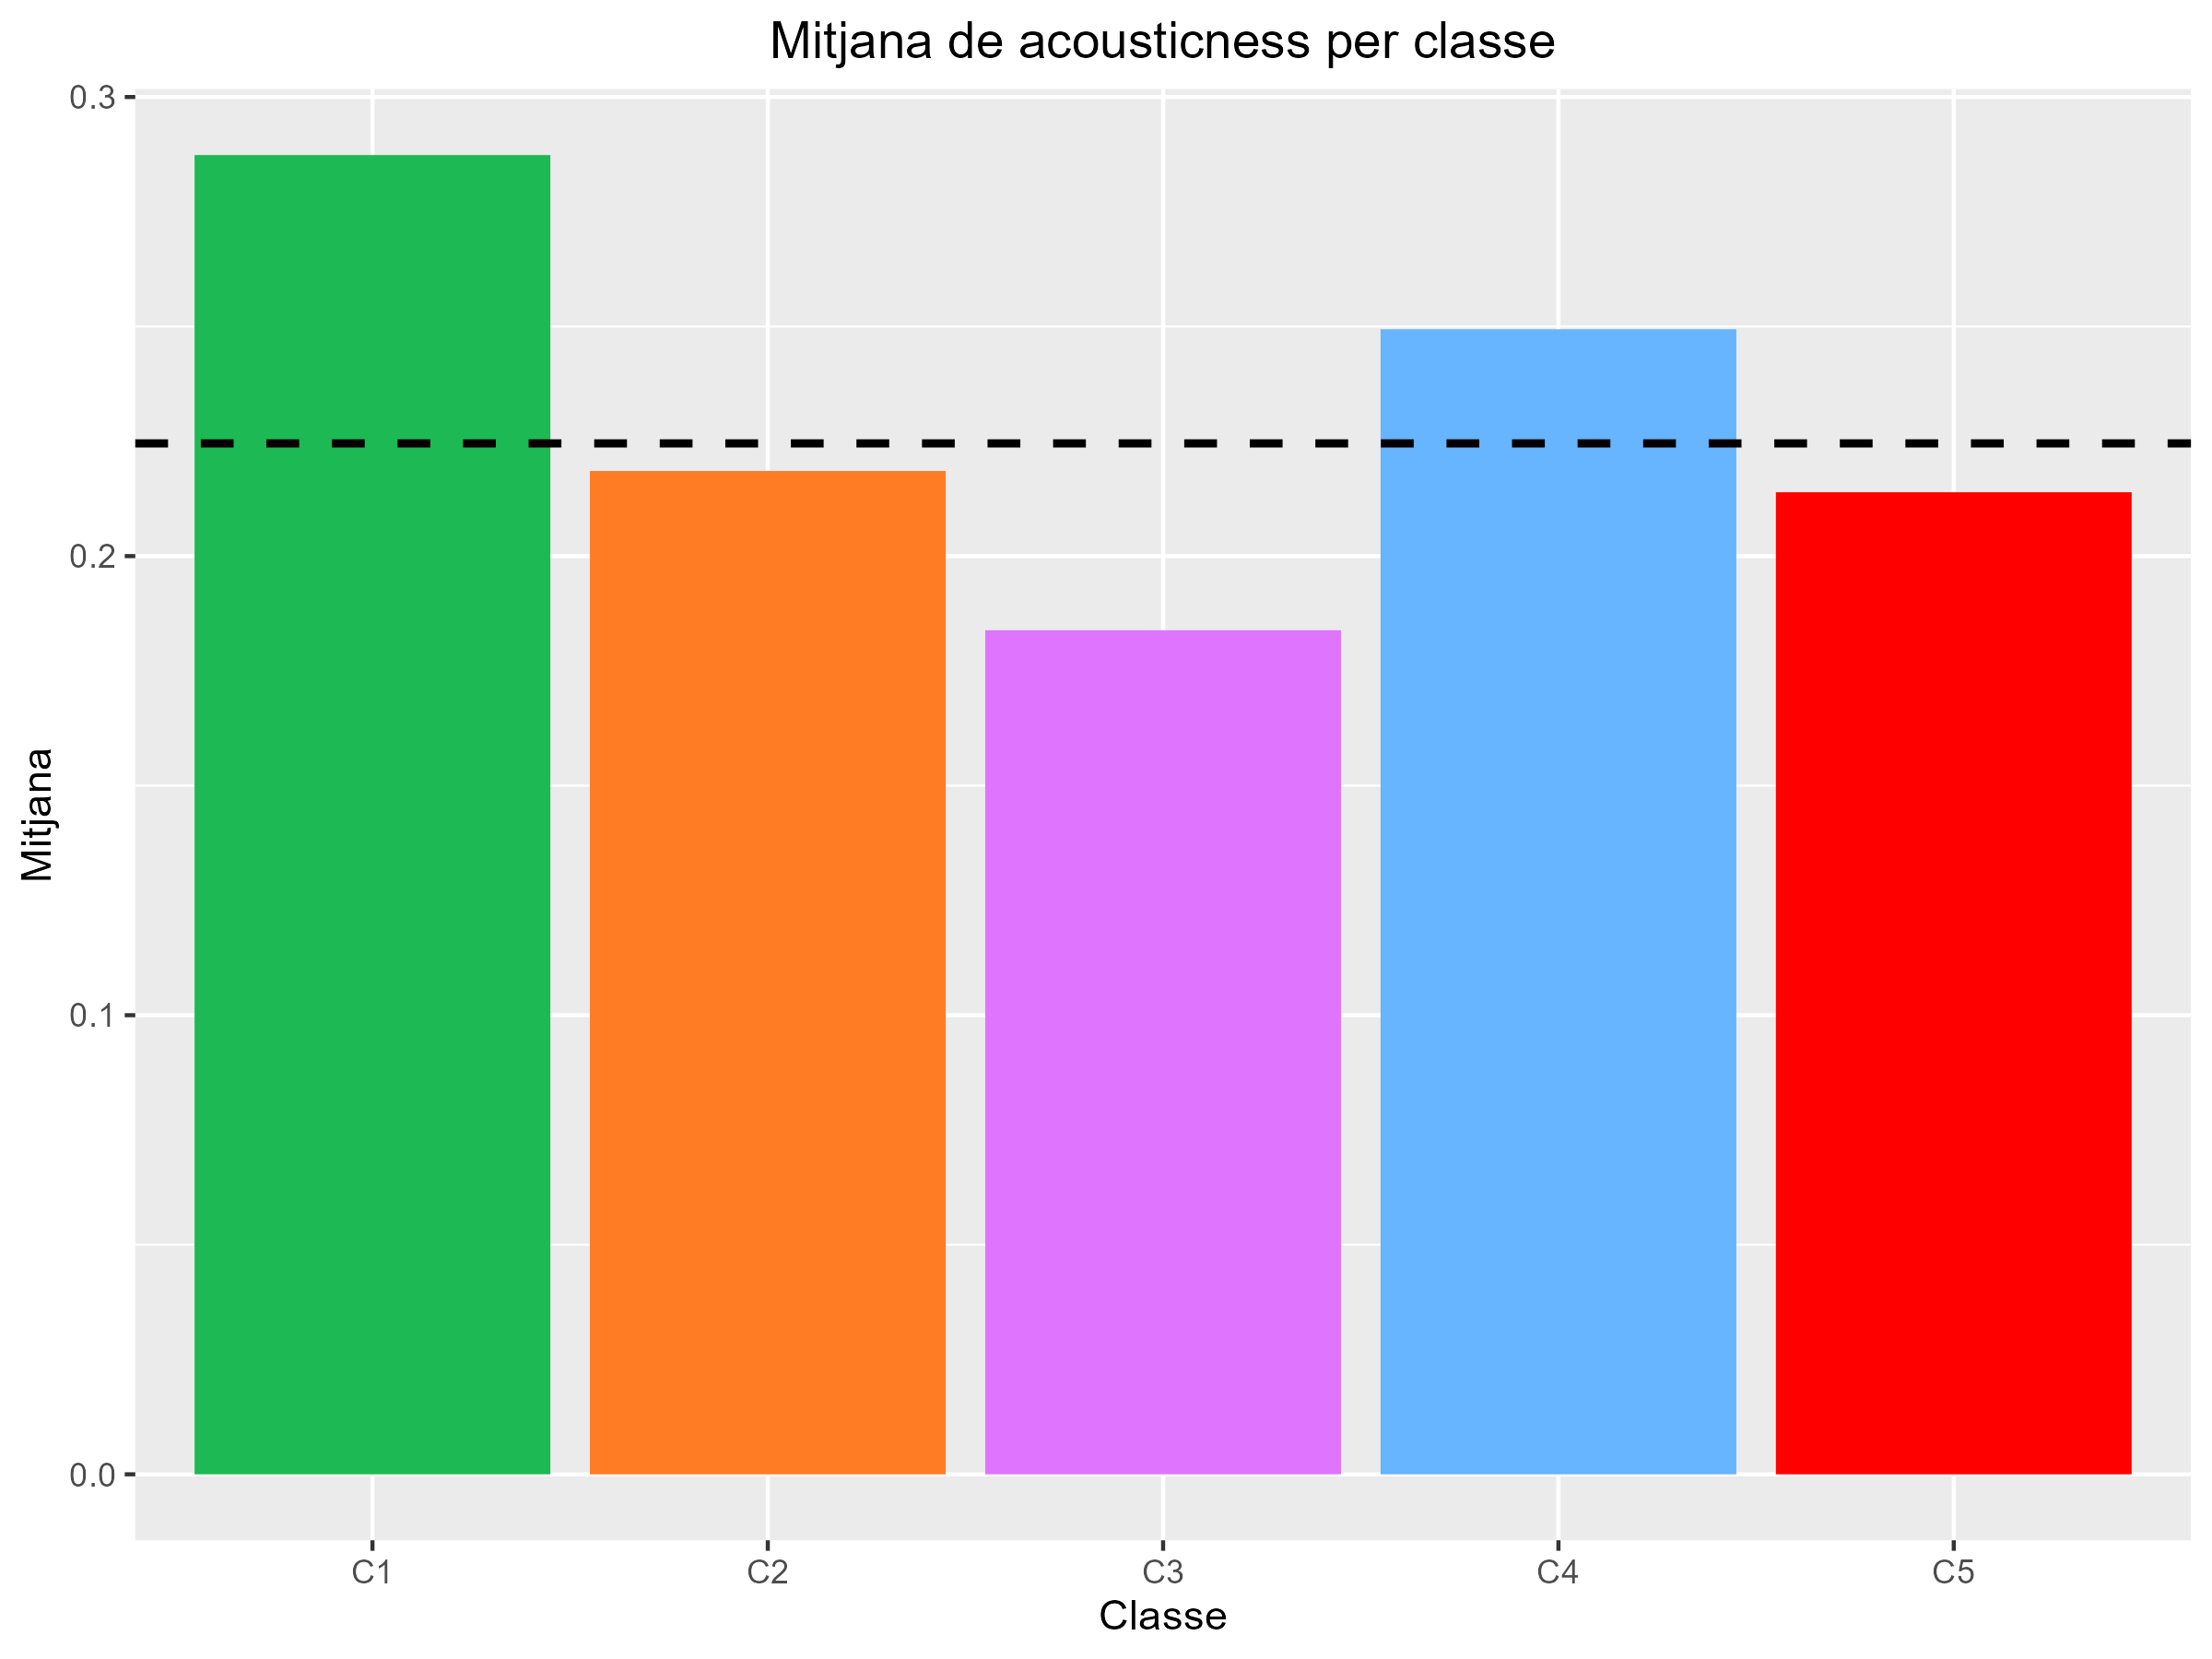
\includegraphics[width=0.95\linewidth]{Images/5_Profiling/numeriques/Num_BarPlot_acousticness.png}
        \caption{Barplot amb les mitjanes \\ d'acousticness per clúster}
        \label{fig:Num_BarPlot_acousticness}
    \end{minipage}%
    \begin{minipage}{.49\textwidth}
        \centering
        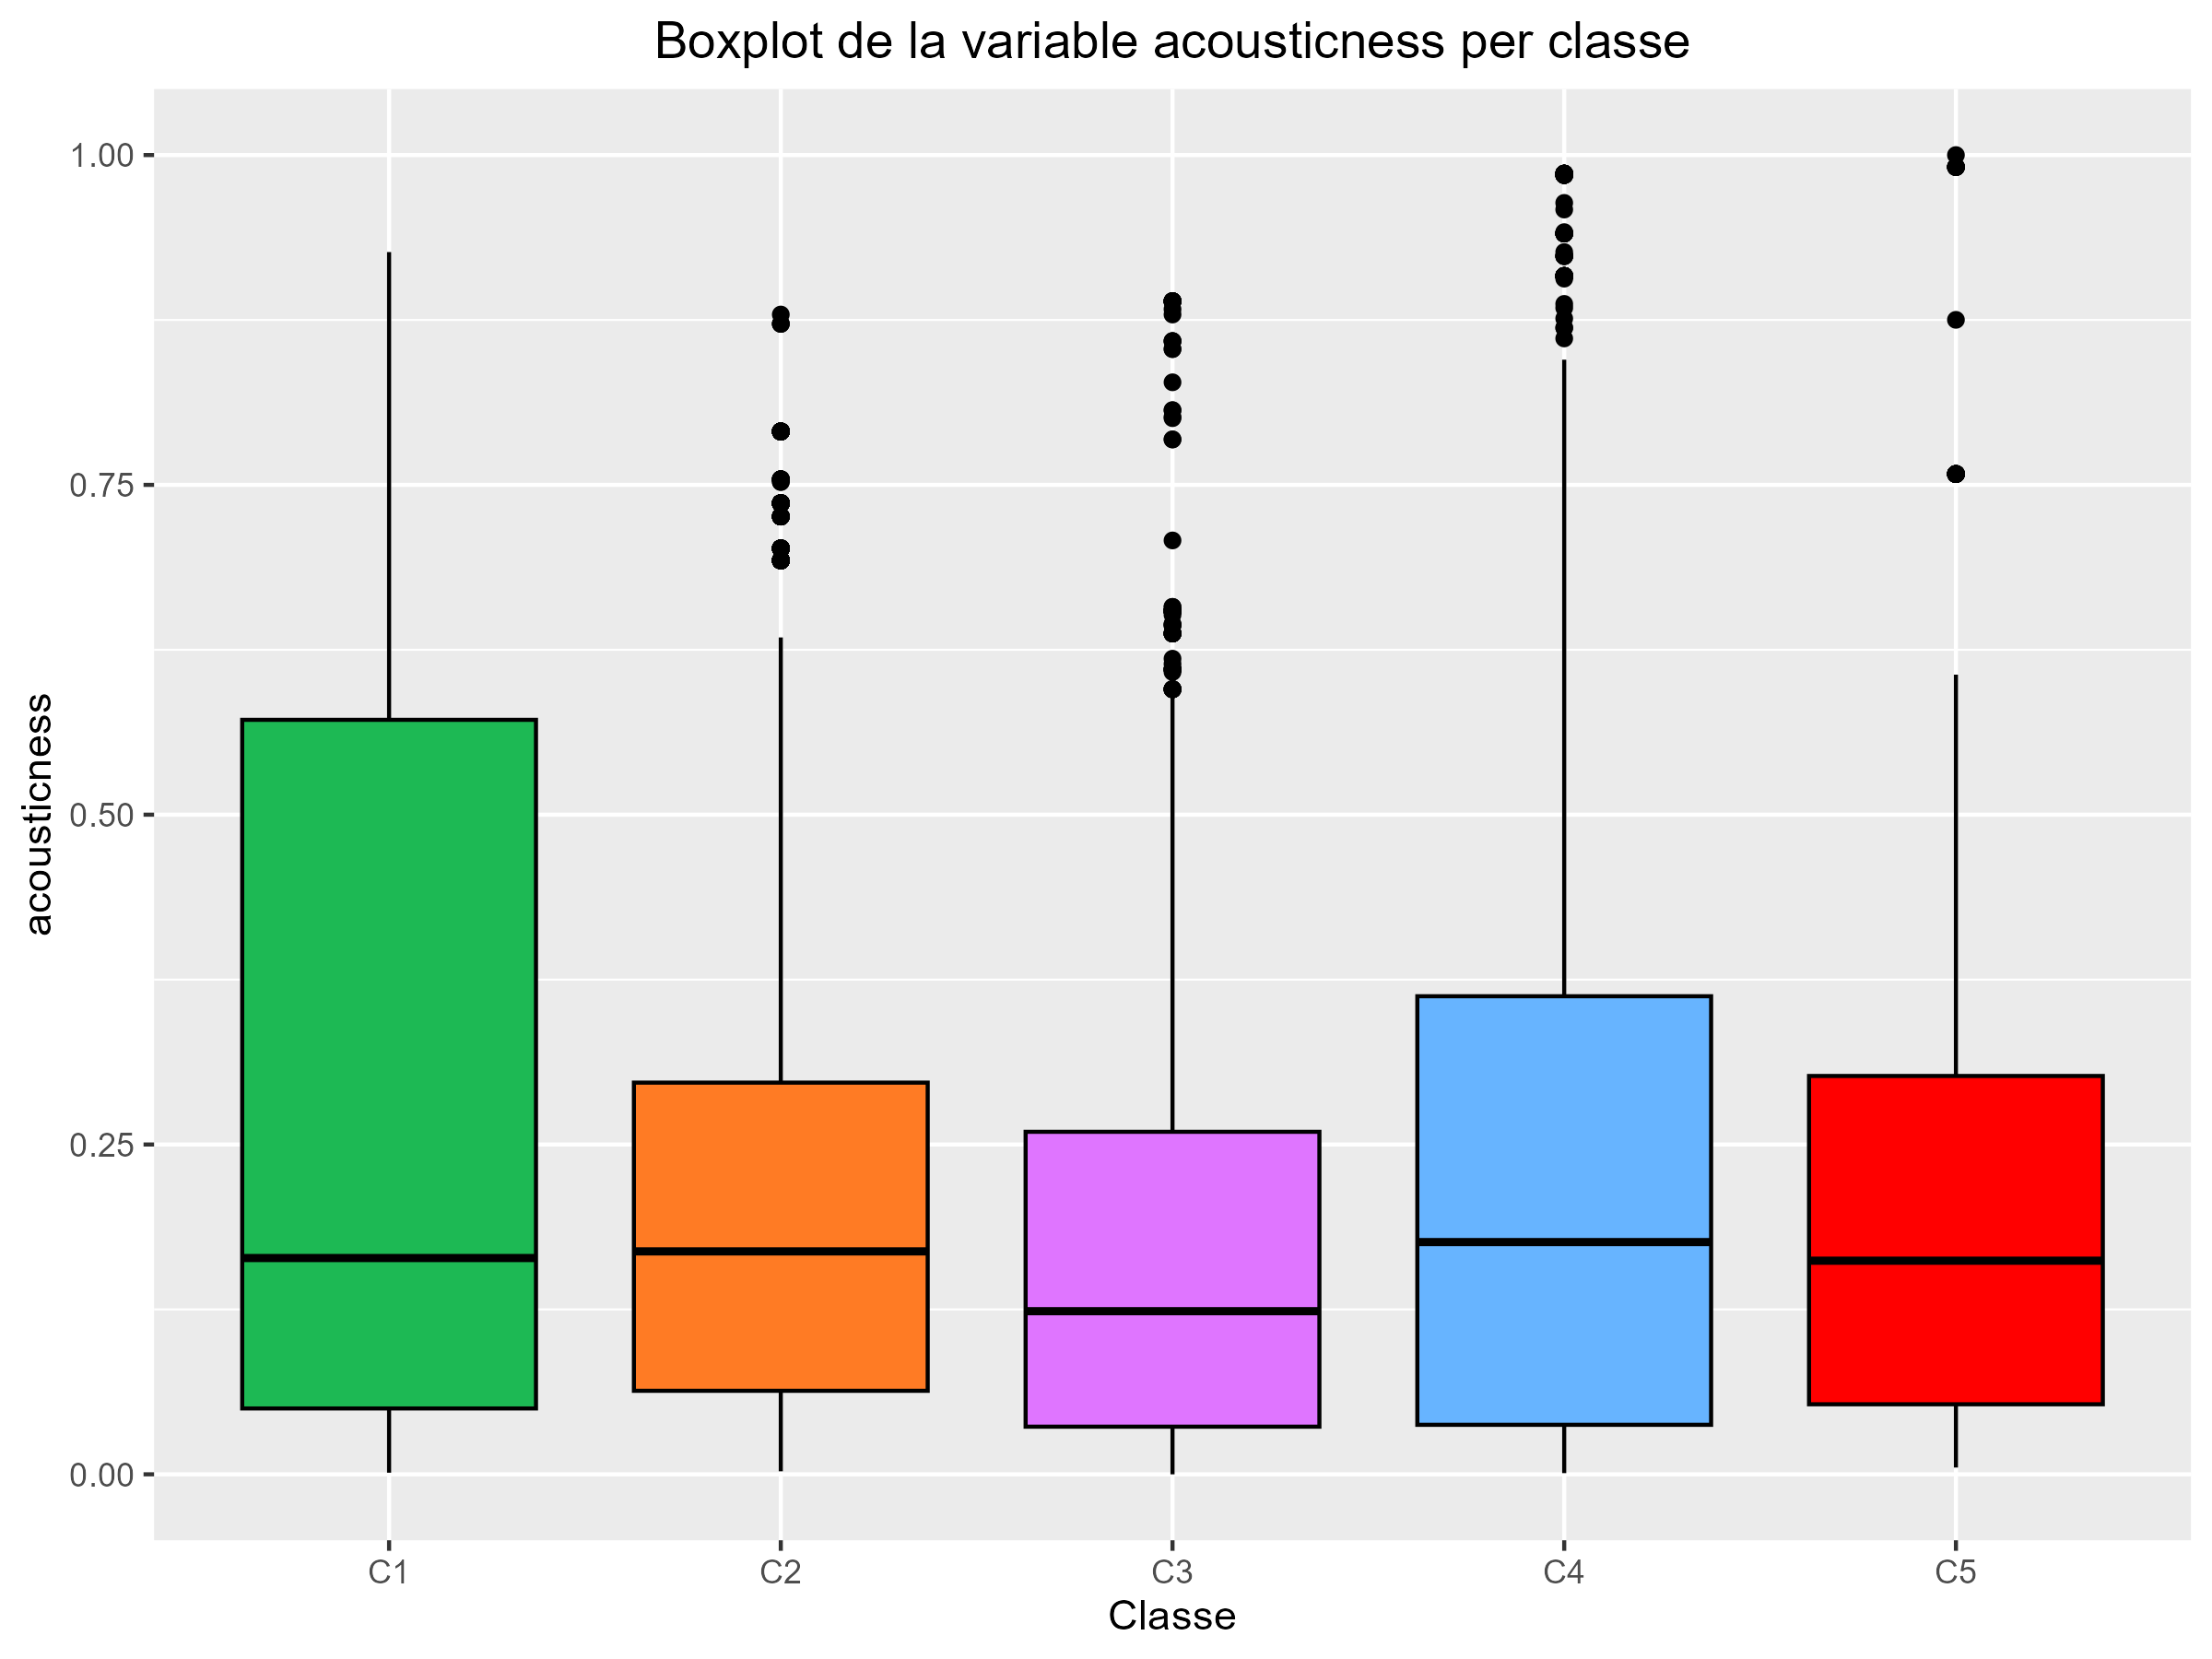
\includegraphics[width=0.95\linewidth]{Images/5_Profiling/numeriques/Num_BoxPlot_acousticness.png}
        \caption{Boxplots d'acousticness per clúster}
        \label{fig:Num_BoxPlot_acousticness}
    \end{minipage}%
\end{figure}

La primera variable en la que ens fixem és l'acousticness. Veiem que la mitjana del primer clúster és molt més alta que la dels altres. Això ens indica que a la primera classe és on hi ha les cançons més aviat acústiques. Les classes dos i cinc tenen la mitjana pràcticament igual que la mitjana total, cosa que vol dir que no els hi afecta lo acústica que és una cançó. Finalment la classe 3 és la que té la mitjana més baixa de la total volent dir que allà hi ha cançons menys acústiques. 

\begin{figure}[H]
\centering
    \begin{minipage}{.49\textwidth}
        \centering
        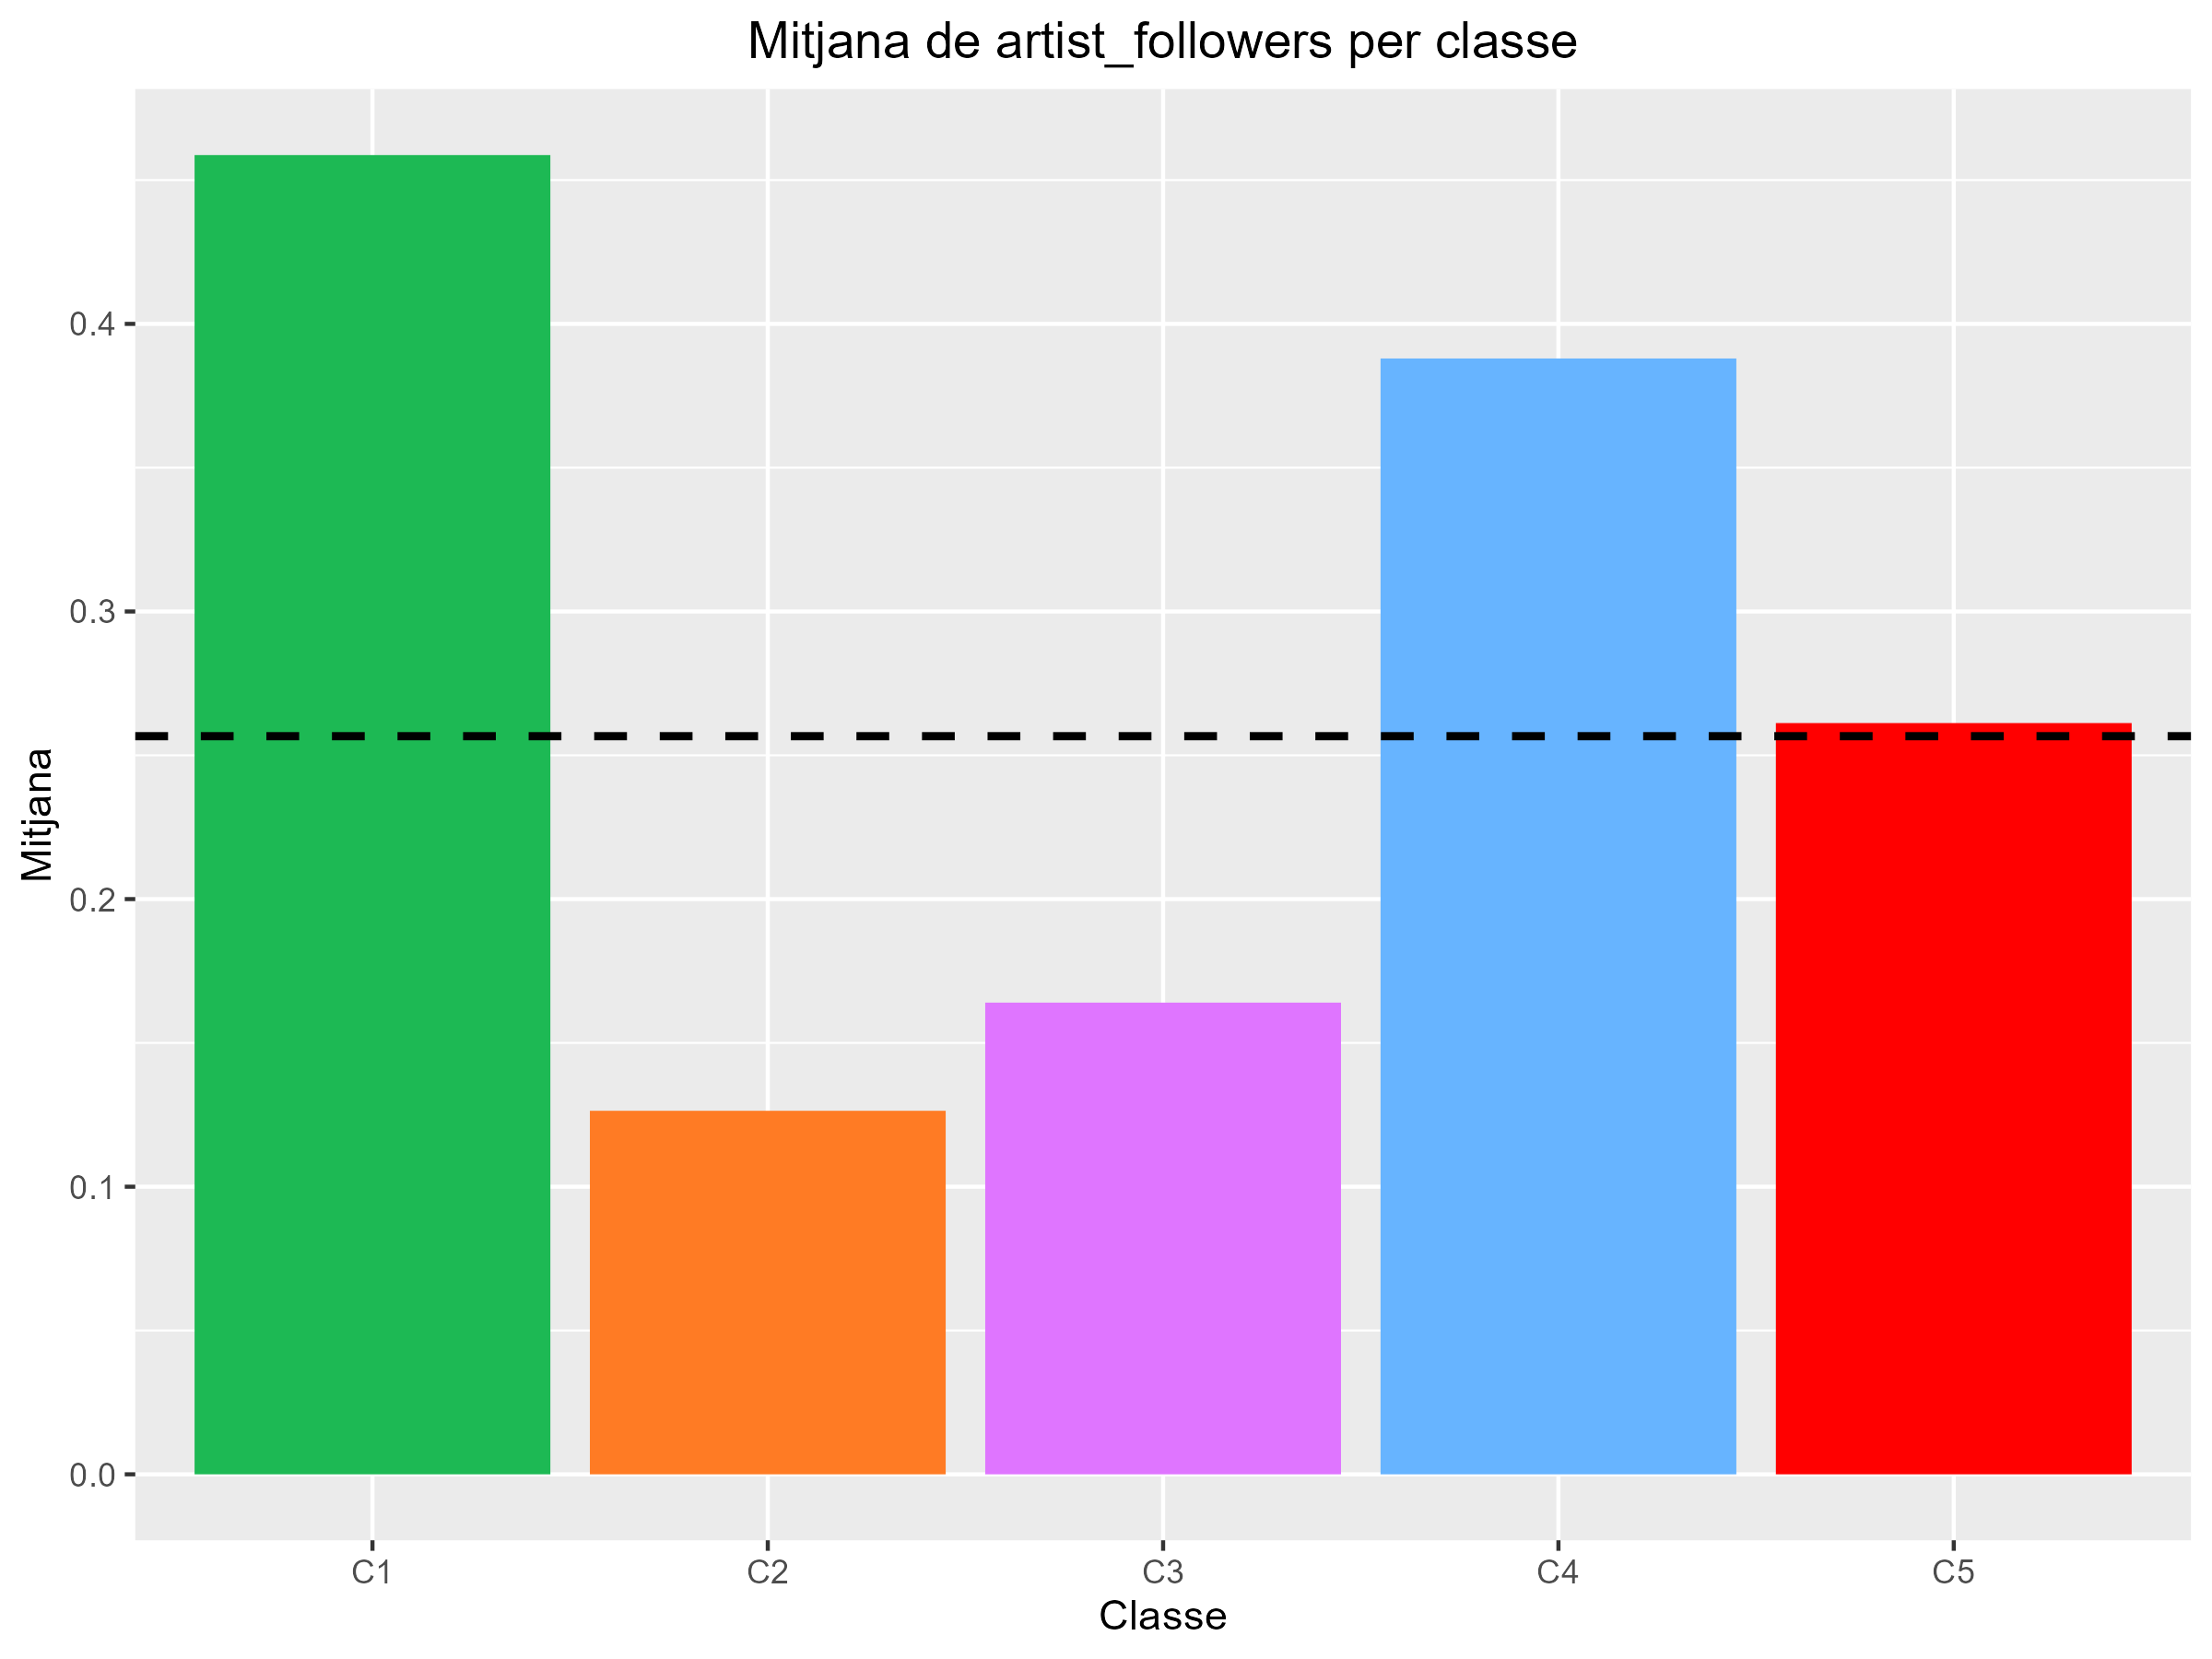
\includegraphics[width=0.95\linewidth]{Images/5_Profiling/numeriques/Num_BarPlot_artist_followers.png}
        \caption{Barplot amb les mitjanes \\ d'artist\_followers per clúster}
        \label{fig:Num_BarPlot_artist_followers}
    \end{minipage}%
    \begin{minipage}{.49\textwidth}
        \centering
        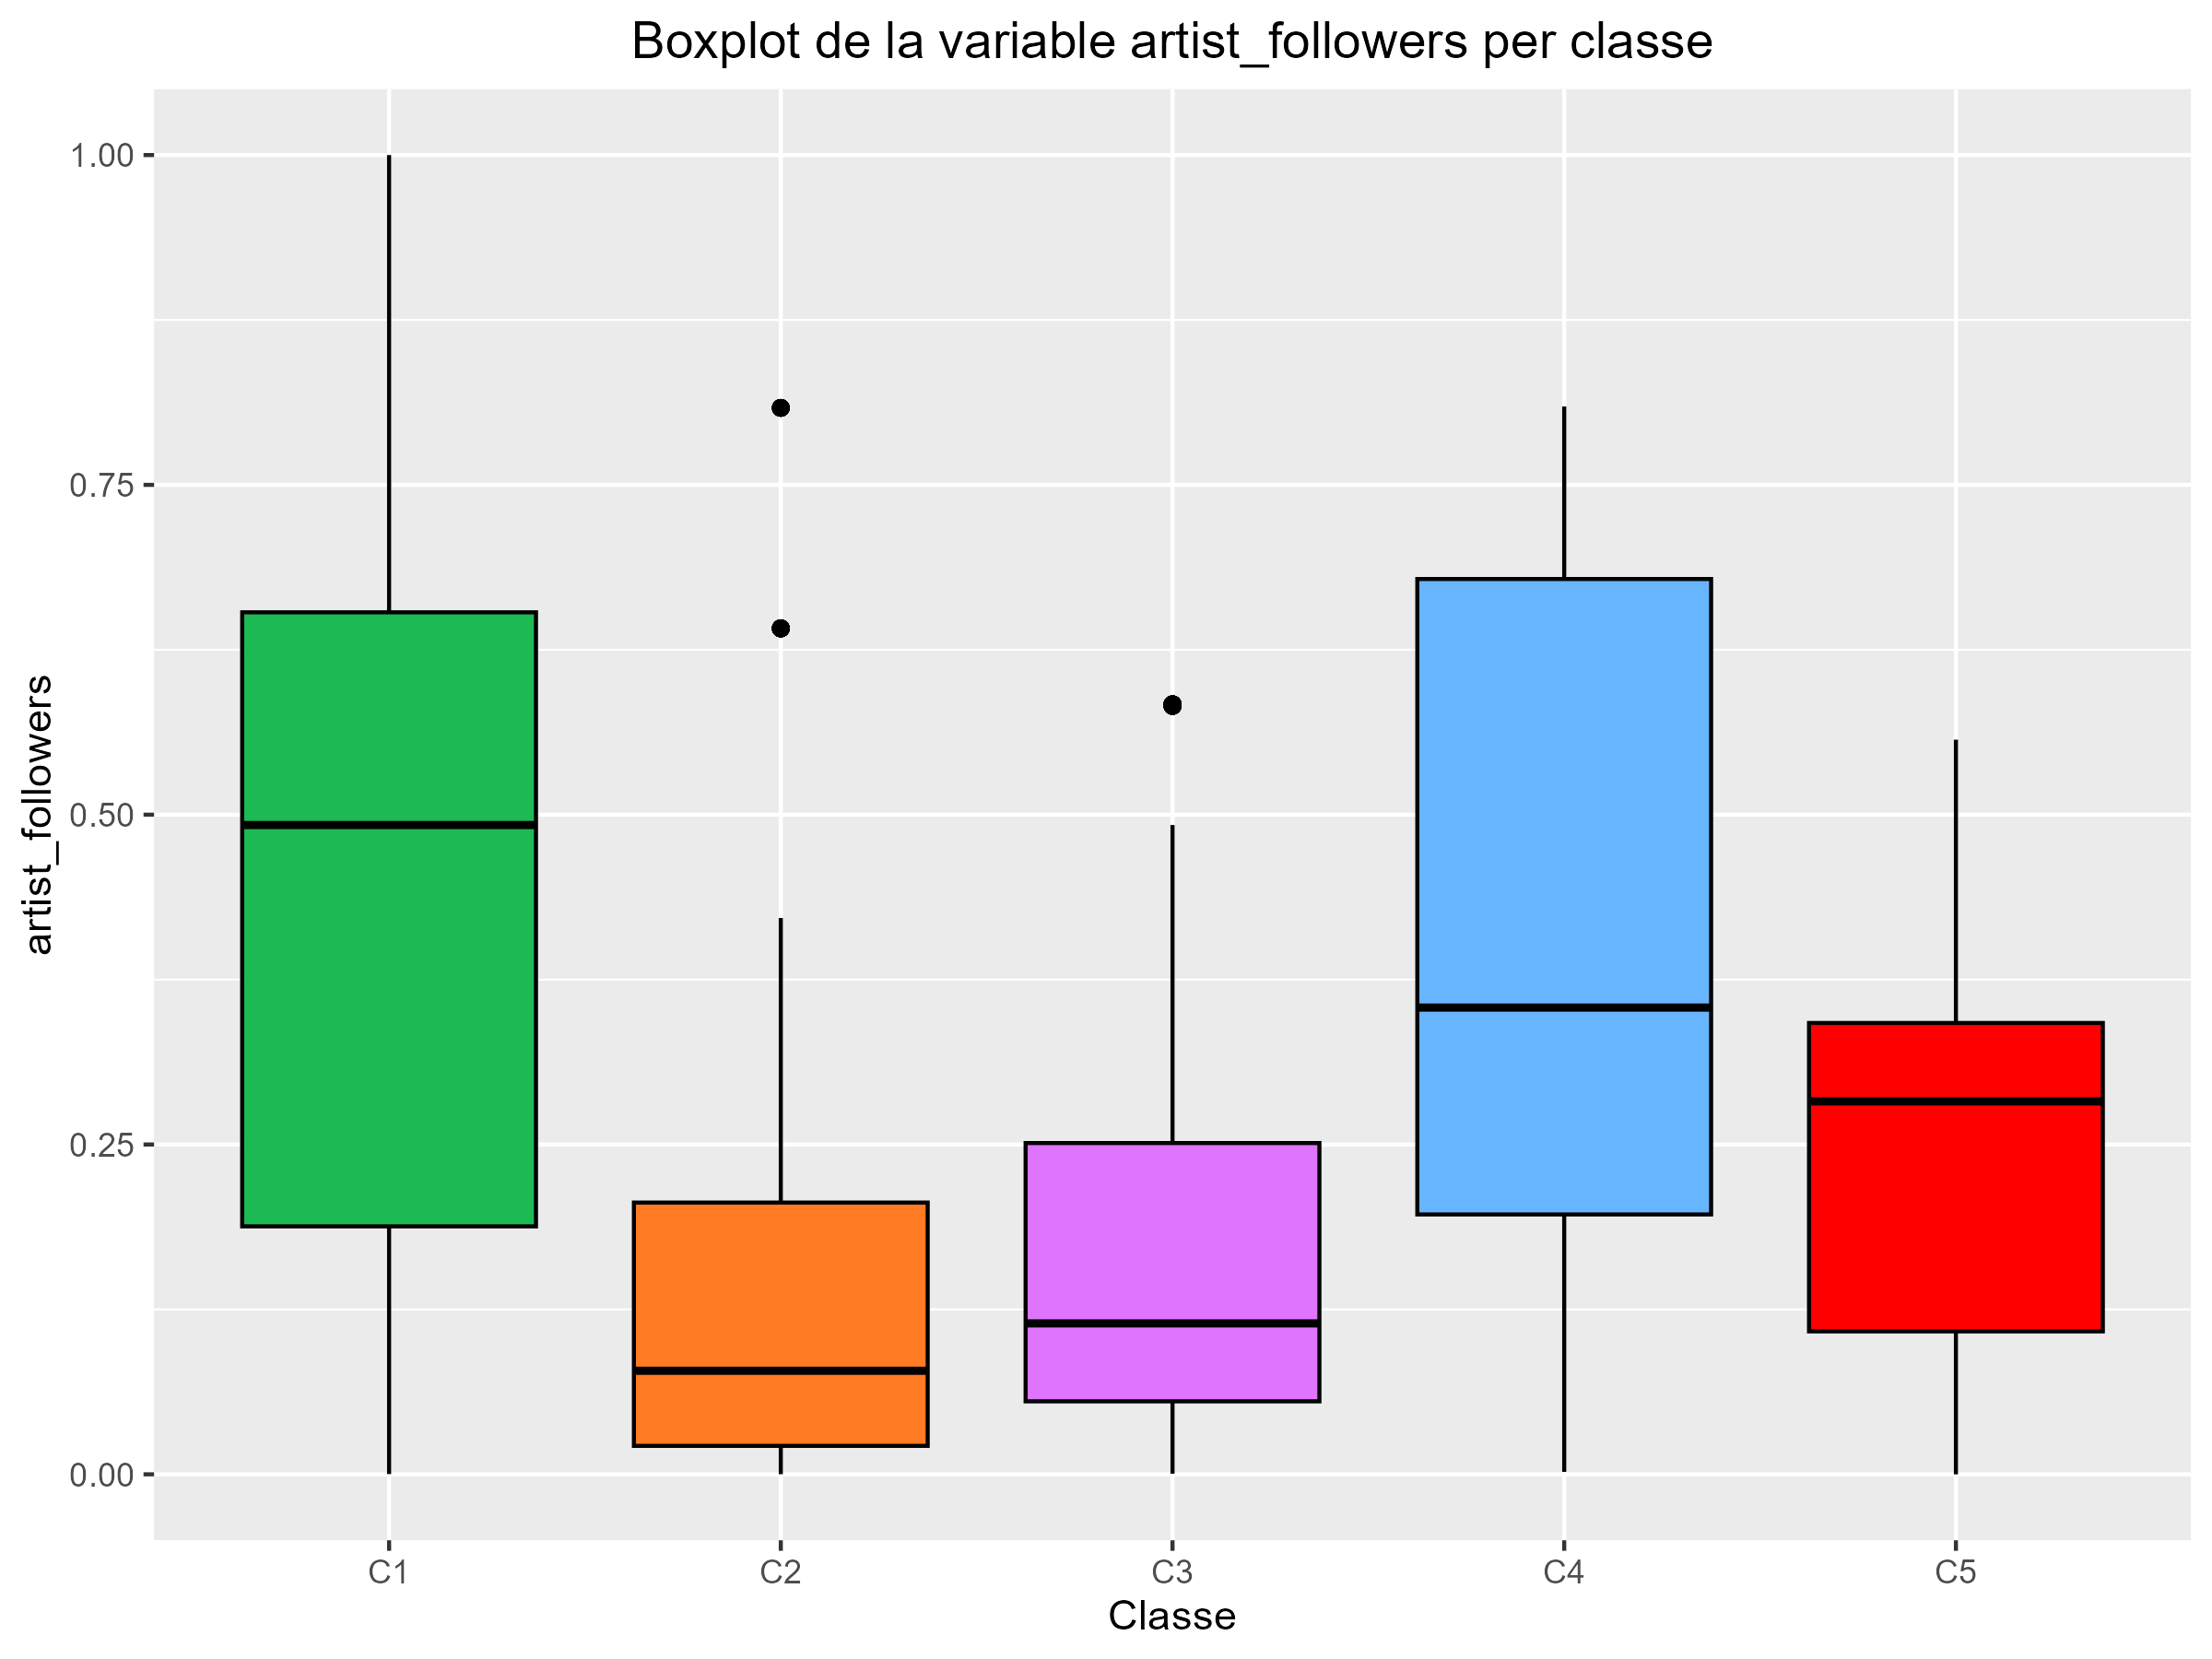
\includegraphics[width=0.95\linewidth]{Images/5_Profiling/numeriques/Num_BoxPlot_artist_followers.png}
        \caption{Boxplots d'artist\_followers per clúster}
        \label{fig:Num_BoxPlot_artist_followers}
    \end{minipage}%
\end{figure}

També es veuen diferències molt significatives entre les mitjanes d'artist\_followers. Veiem que, amb molta diferència, la classe u és on hi ha els artistes amb més followers. La classe quatre també té artistes amb molts seguidors, i hi ha molta diferència amb els clústers 2 i 3 que tenen la mitjana molt baixa i per tant tenen molts menys seguidors. Finalment, la classe 5 té la mateixa mitjana que la total indicant que no li afecten els seguidors de l'artista. 

\begin{figure}[H]
\centering
    \begin{minipage}{.49\textwidth}
        \centering
        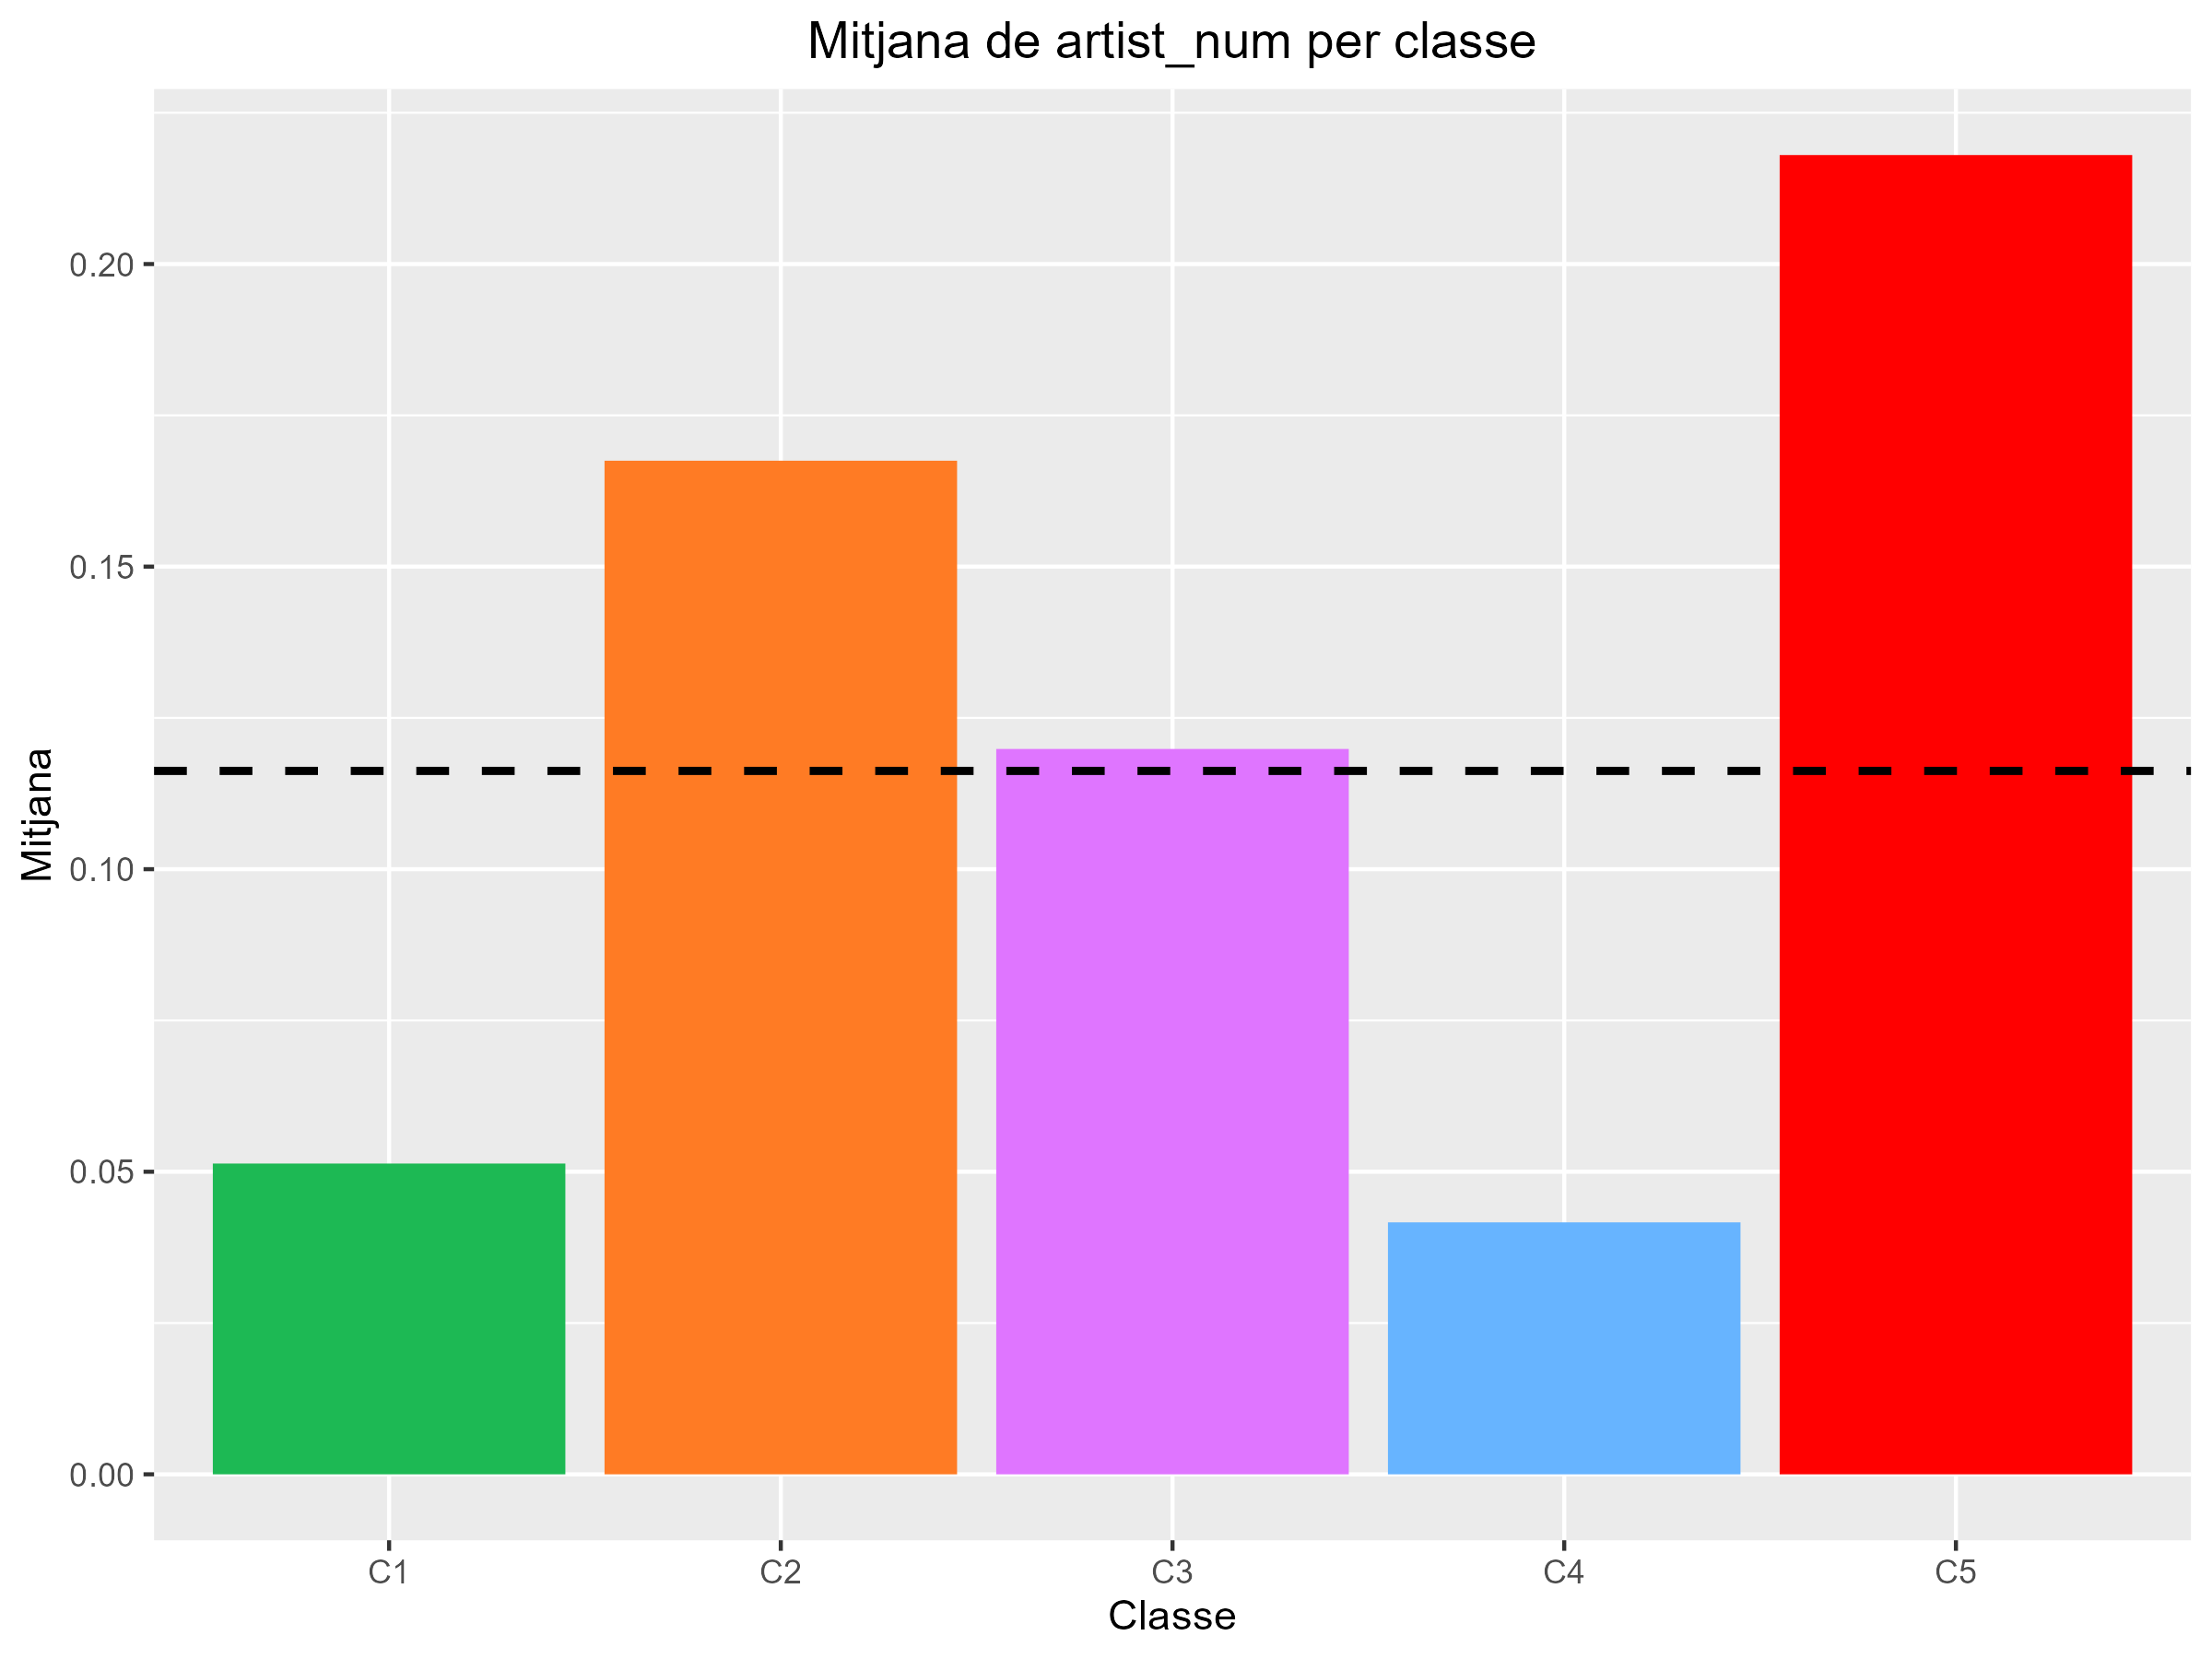
\includegraphics[width=0.95\linewidth]{Images/5_Profiling/numeriques/Num_BarPlot_artist_num.png}
        \caption{Barplot amb les mitjanes \\ d'artist\_num per clúster}
        \label{fig:Num_BarPlot_artist_num}
    \end{minipage}%
    \begin{minipage}{.49\textwidth}
        \centering
        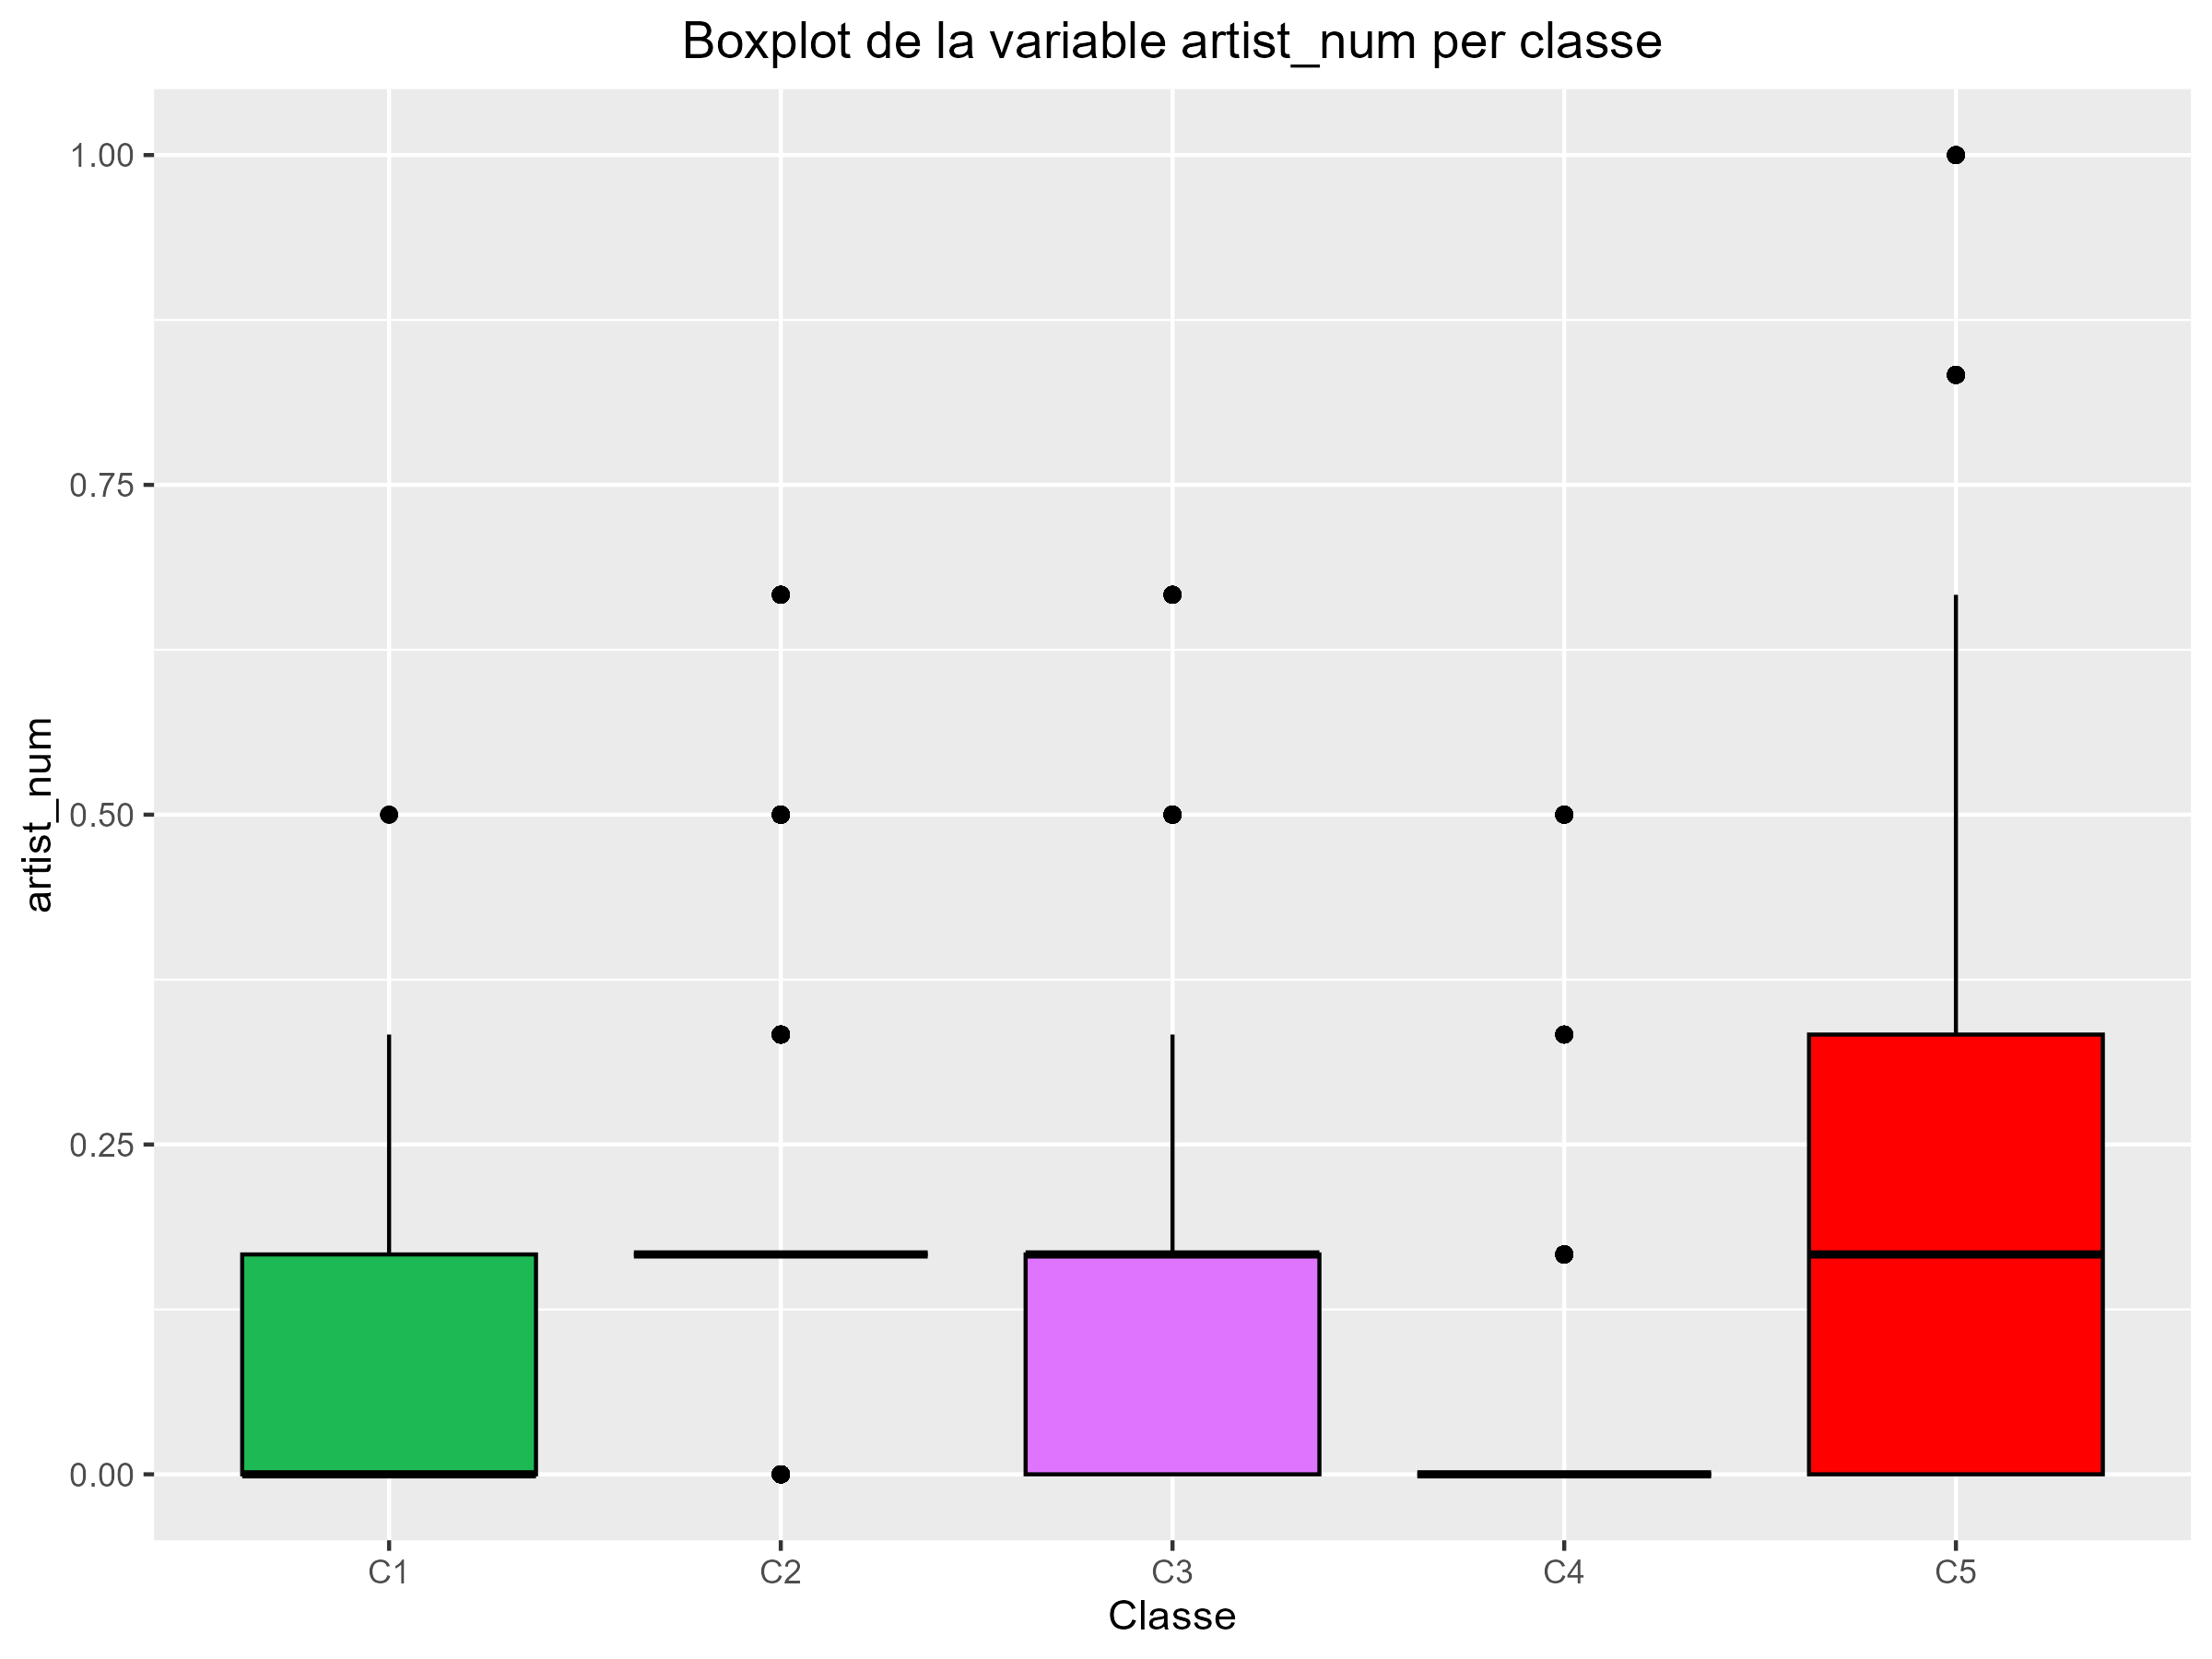
\includegraphics[width=0.95\linewidth]{Images/5_Profiling/numeriques/Num_BoxPlot_artist_num.png}
        \caption{Boxplots d'artist\_num per clúster}
        \label{fig:Num_BoxPlot_artist_num}
    \end{minipage}%
\end{figure}
Artist\_num també veiem que és una variable que està afectant a la creació dels nostres clústers. Veiem que els clústers amb les mitjanes més baixes són el 1 i el 4, i això indica que tenen cançons que involucren a pocs artistes, o menys que la resta. En canvi, els clústers 2 i 5, sobretot el 5, tenen la mitjana molt més alta, i observant el boxplot trobem que allà és on estan les cançons que tenen, en general, molts més artistes colaborant. Hi ha una gran variabilitat en el nombre d'artistes que colaboren en aquest últim clúster. 

\begin{figure}[H]
\centering
    \begin{minipage}{.49\textwidth}
        \centering
        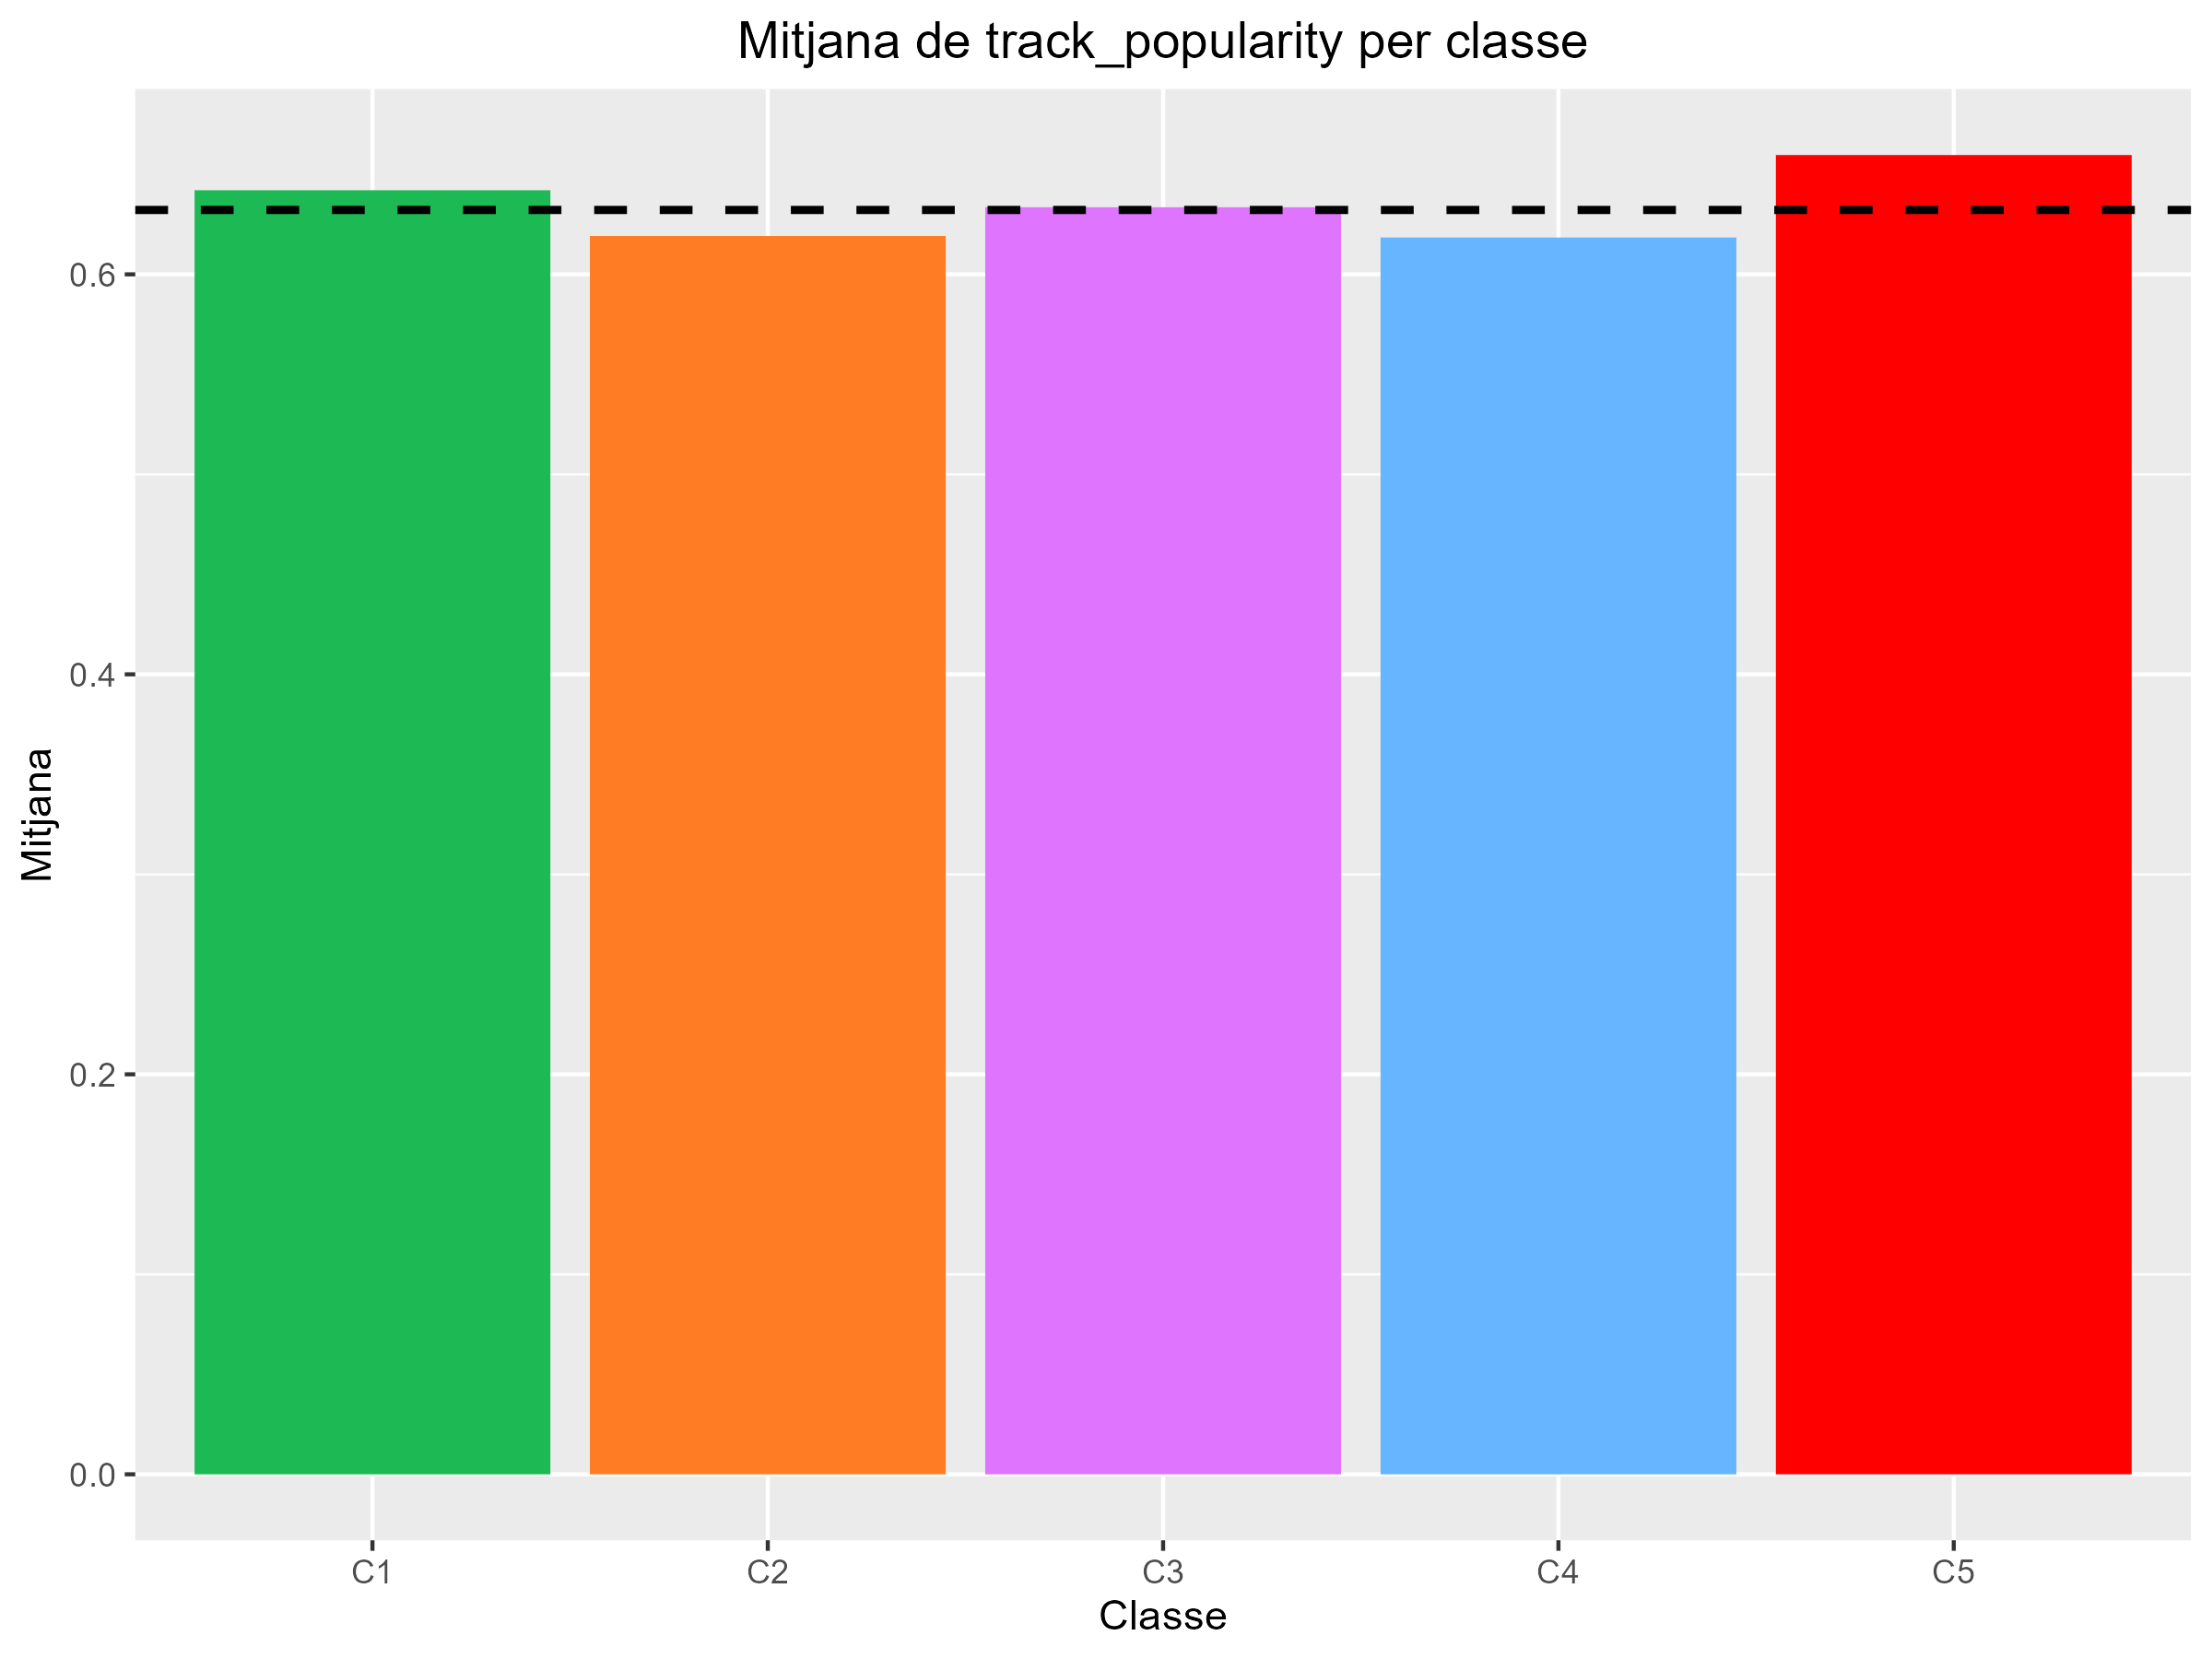
\includegraphics[width=0.95\linewidth]{Images/5_Profiling/numeriques/Num_BarPlot_track_popularity.png}
        \caption{Barplot amb les mitjanes \\ d'track\_popularity per clúster}
        \label{fig:Num_BarPlot_track_popularity}
    \end{minipage}%
    \begin{minipage}{.49\textwidth}
        \centering
        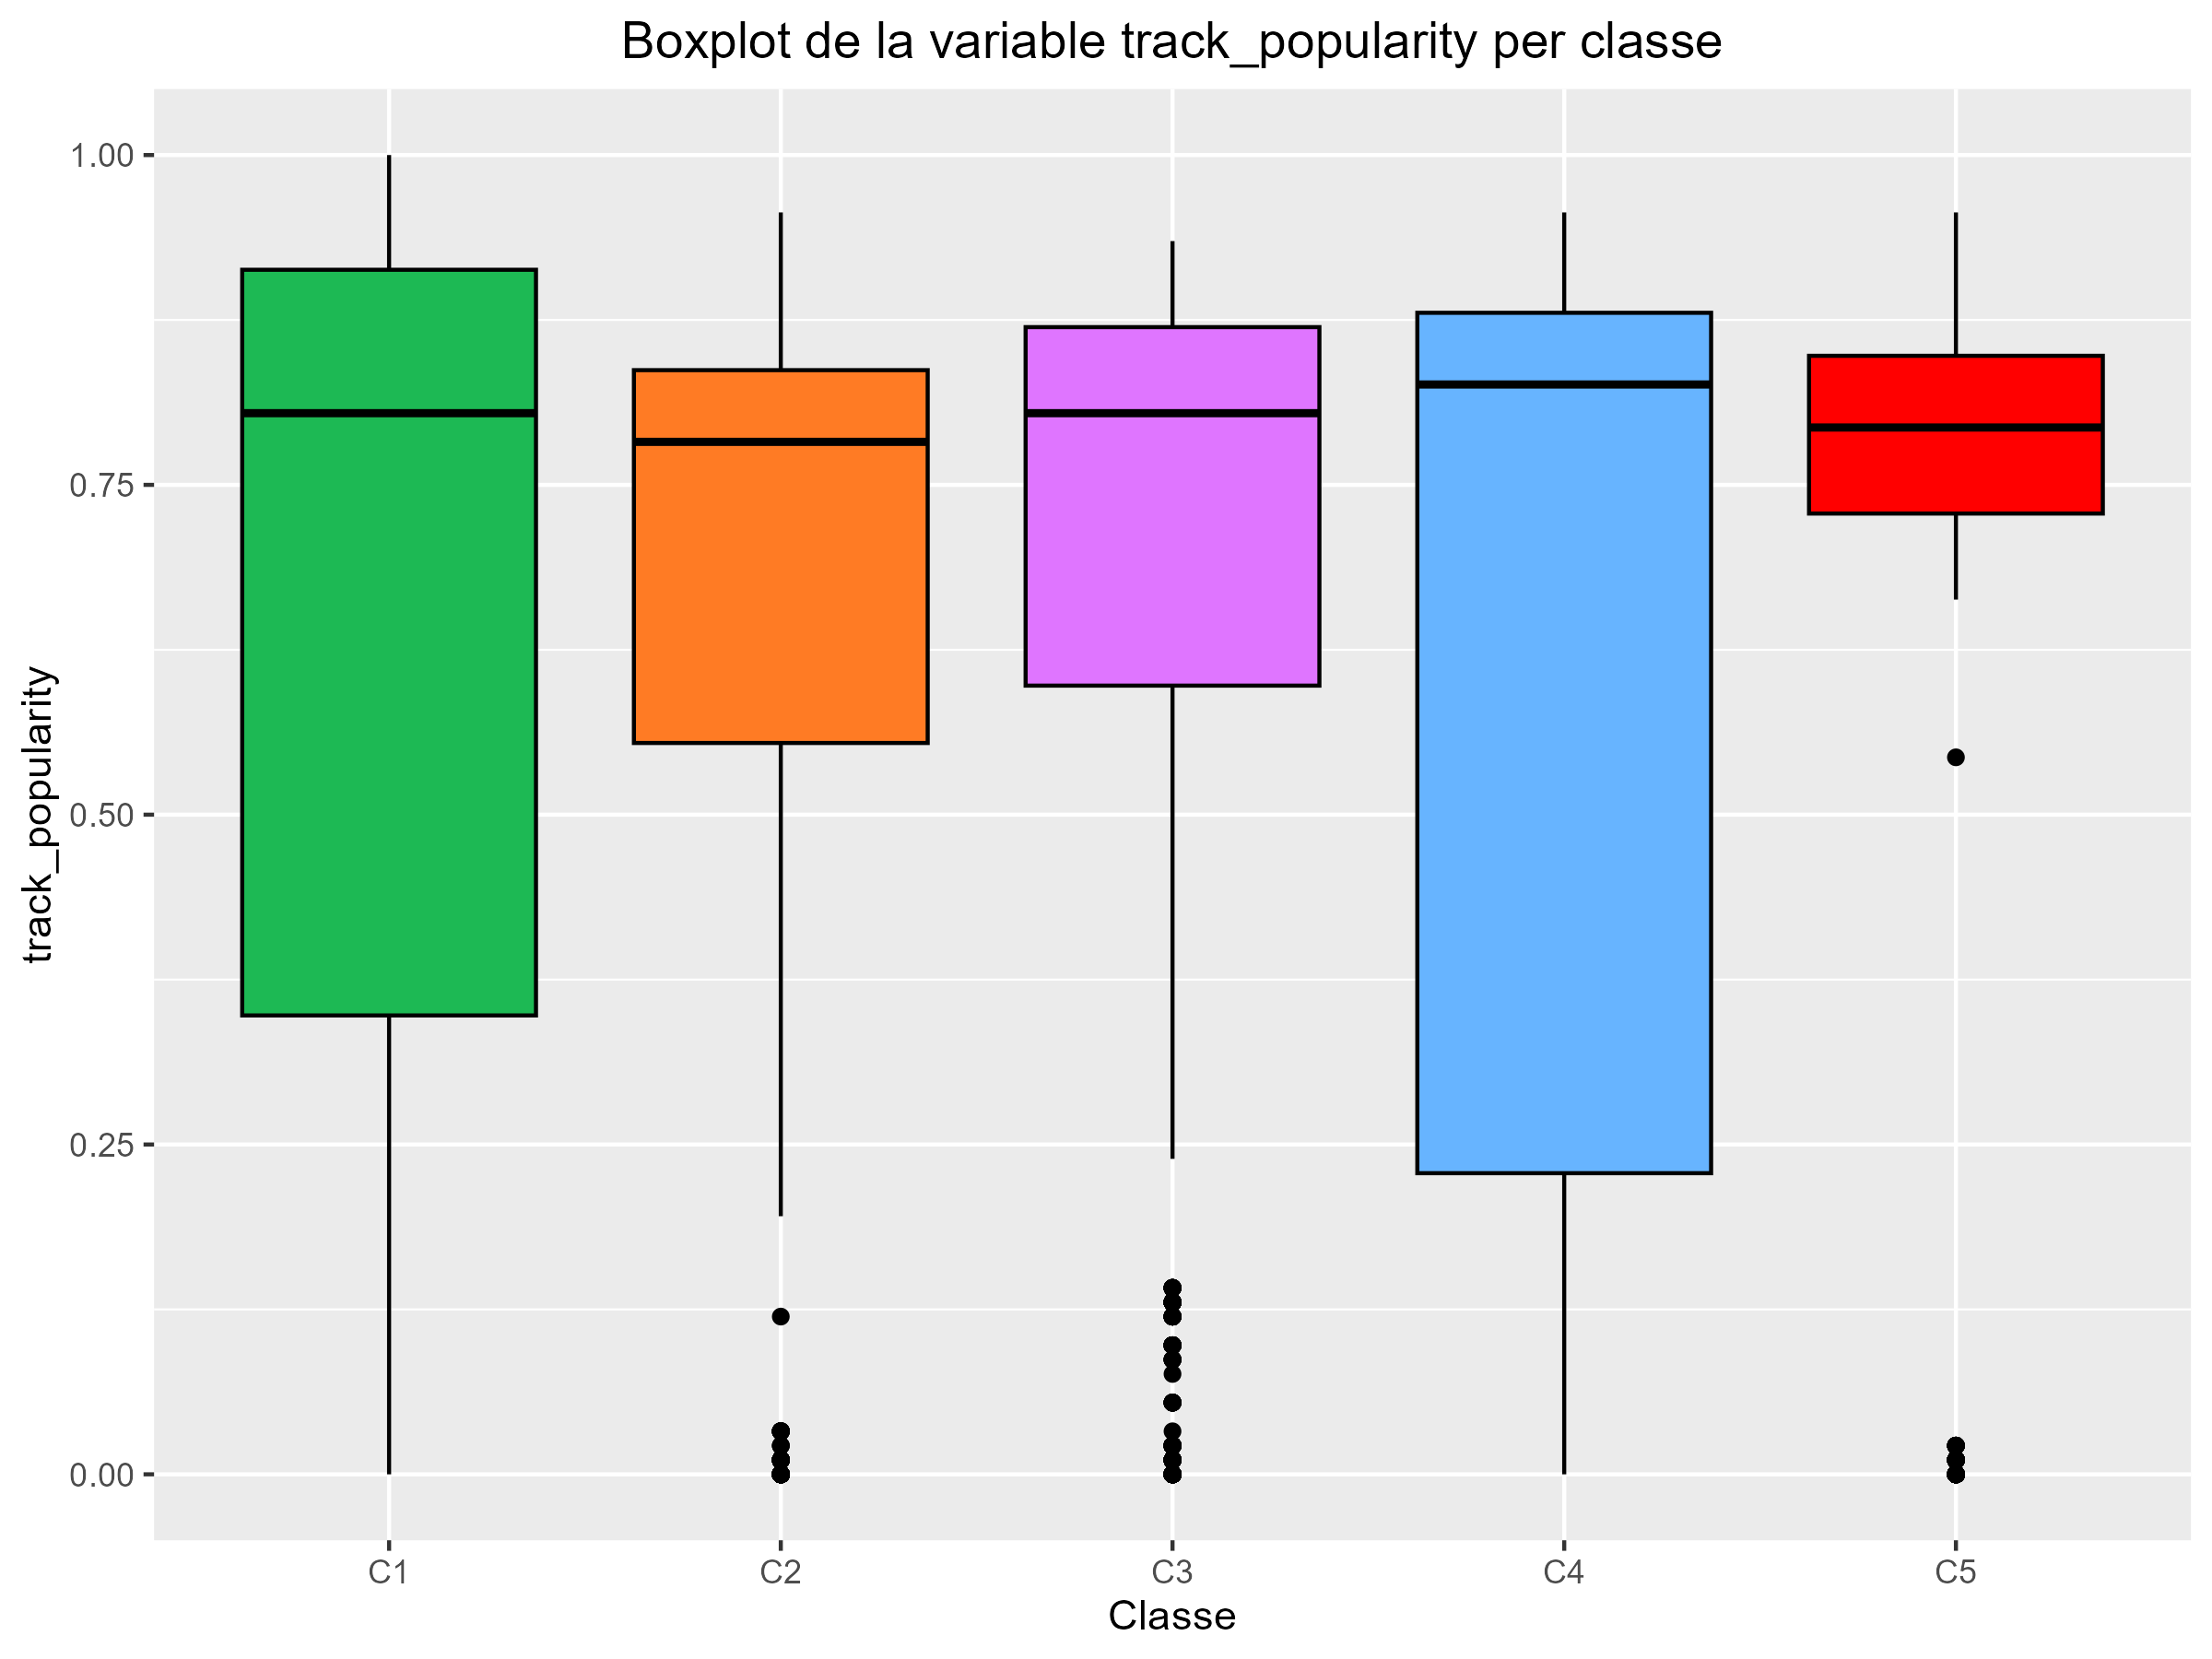
\includegraphics[width=0.95\linewidth]{Images/5_Profiling/numeriques/Num_BoxPlot_track_popularity.png}
        \caption{Boxplots d'track\_popularity per clúster}
        \label{fig:Num_BoxPlot_track_popularity}
    \end{minipage}%
\end{figure}

Una variable que ens ha sorprès molt és la variable track\_popularity, ja que l'any passat, els clústers es van dividir molt segons les popularitats de les cançons i dels albums i aquest any tots tenien mitjanes semblants. Tot i que al Barplot veiem que les mitjanes són totes extremadament semblants a la total, al Boxplot es descobreix que els clústers 1 i 4 tenen més variabilitat de les dades i allà és on es troben les cançons amb una mica menys de popularitat. 

\begin{figure}[H]
\centering
    \begin{minipage}{.49\textwidth}
        \centering
        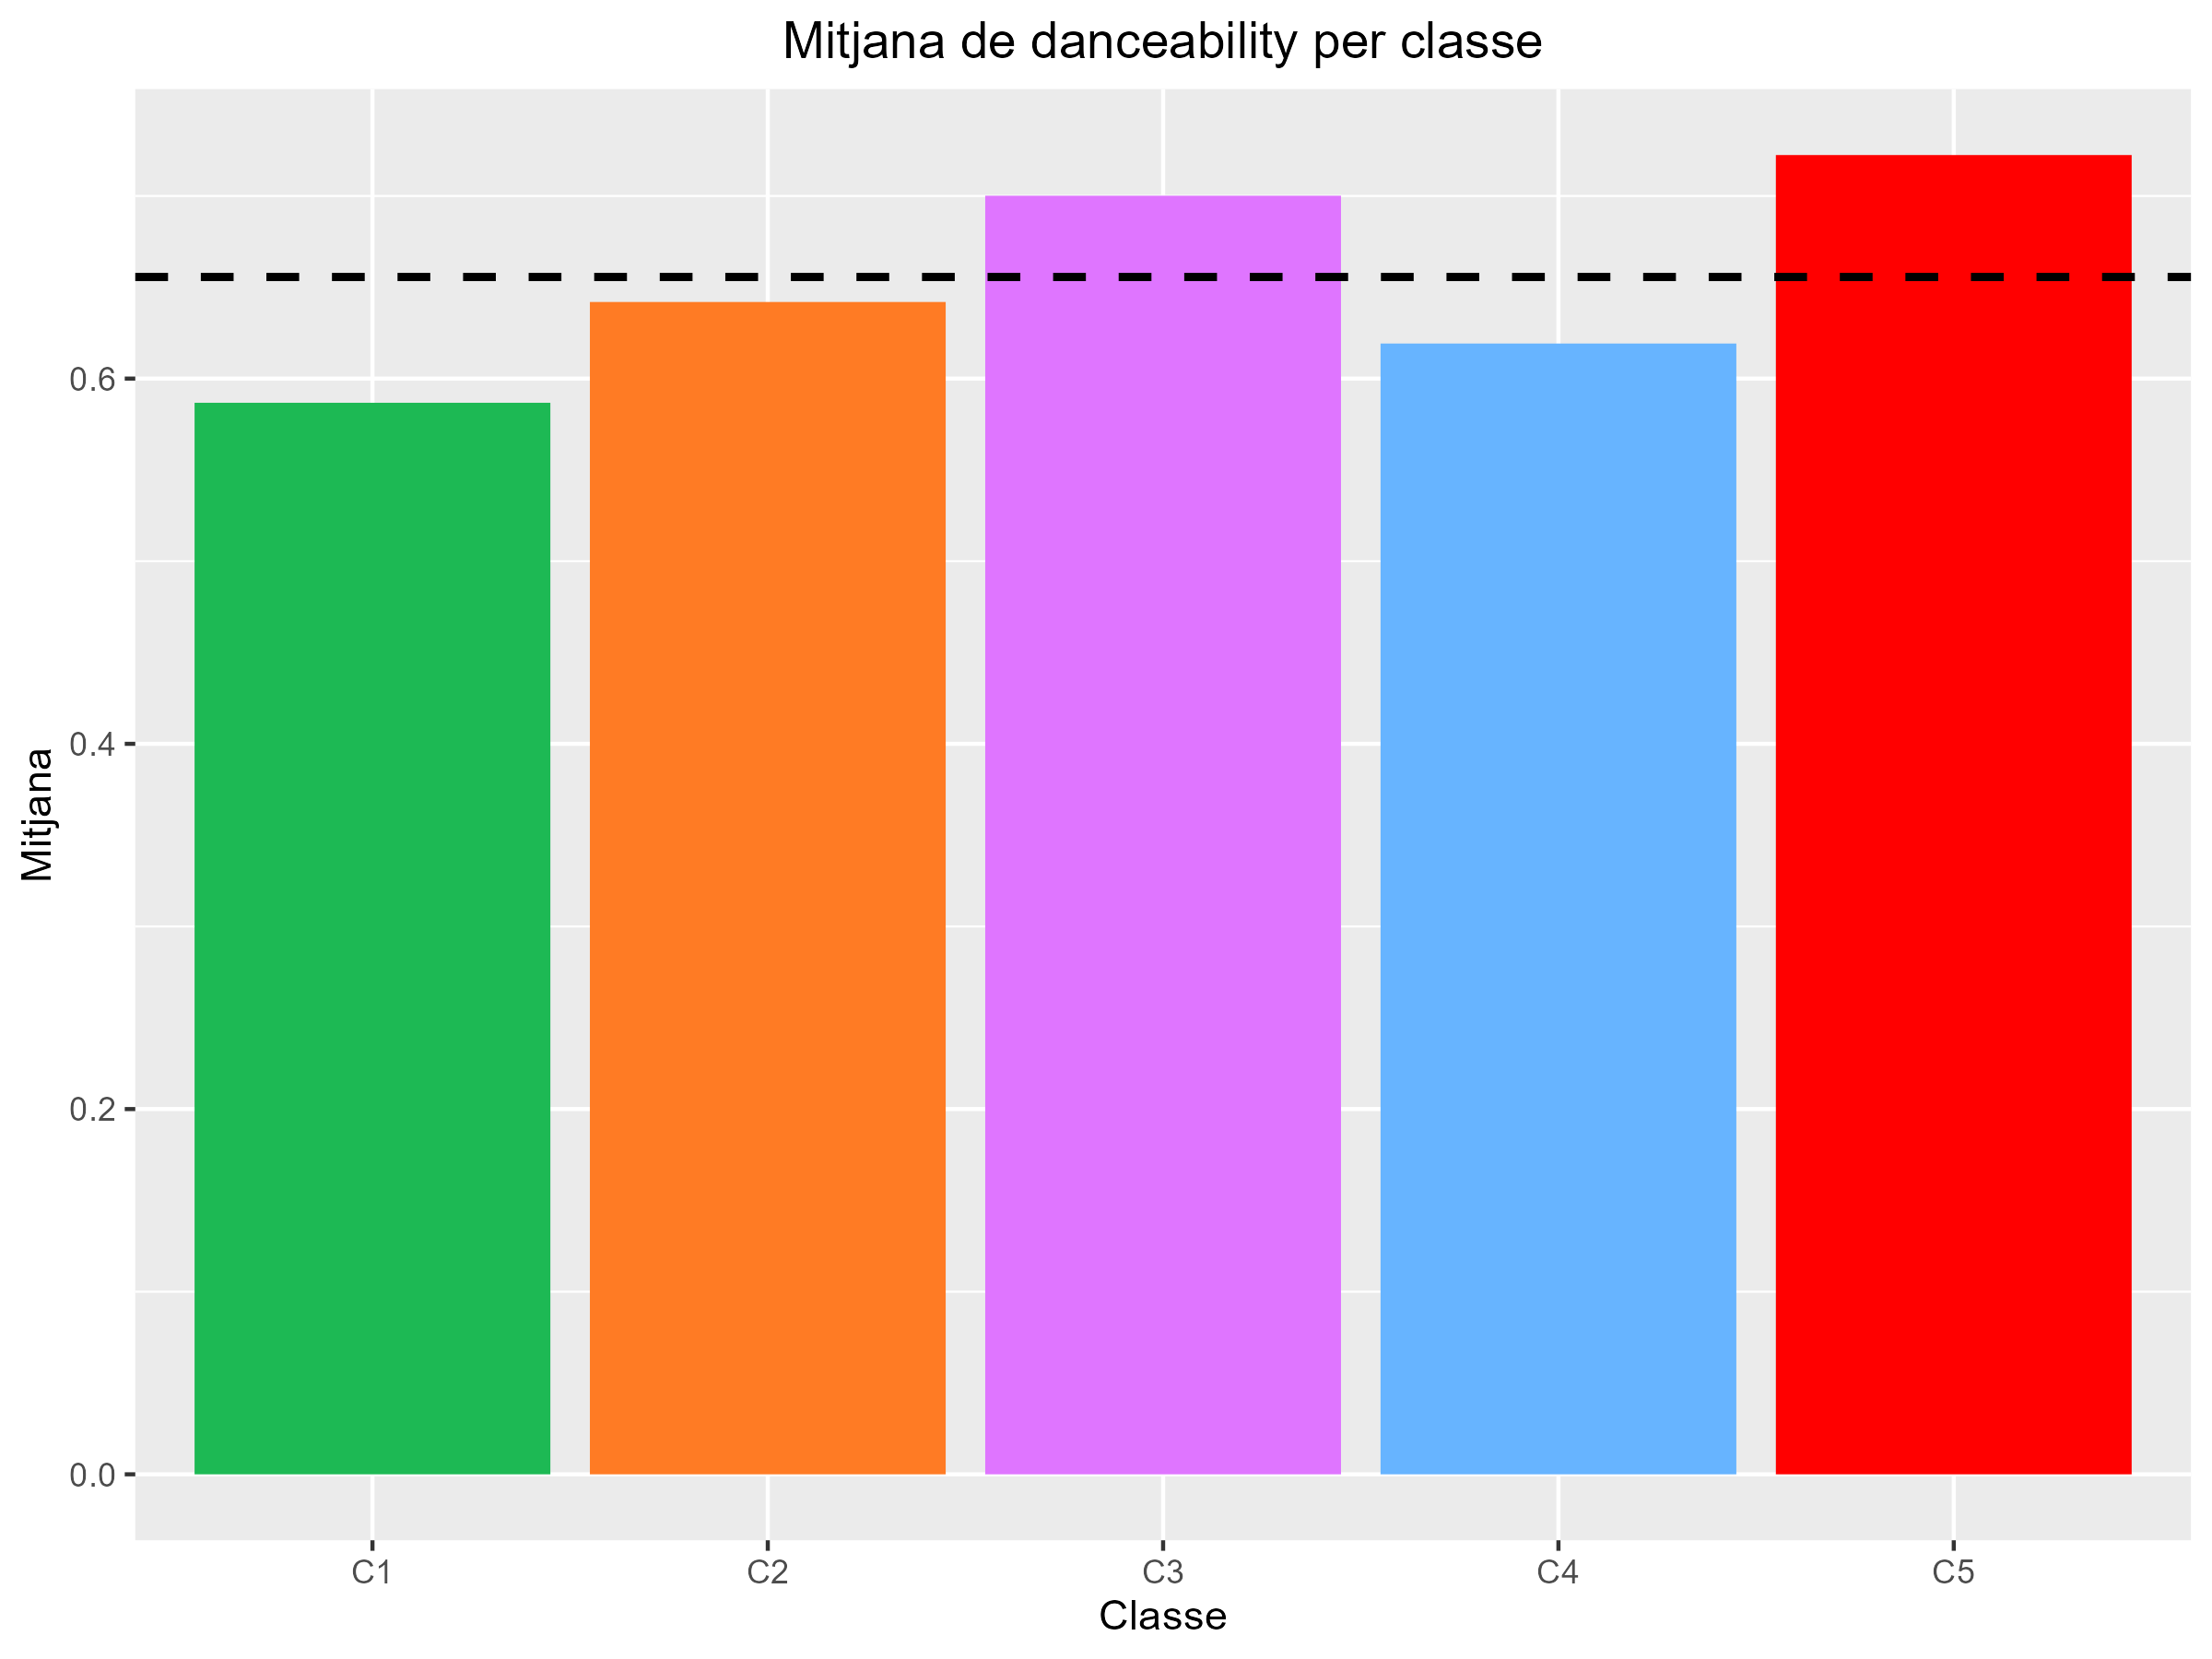
\includegraphics[width=0.95\linewidth]{Images/5_Profiling/numeriques/Num_BarPlot_danceability.png}
        \caption{Barplot amb les mitjanes \\ de danceability per clúster}
        \label{fig:Num_BarPlot_danceability}
    \end{minipage}%
    \begin{minipage}{.49\textwidth}
        \centering
        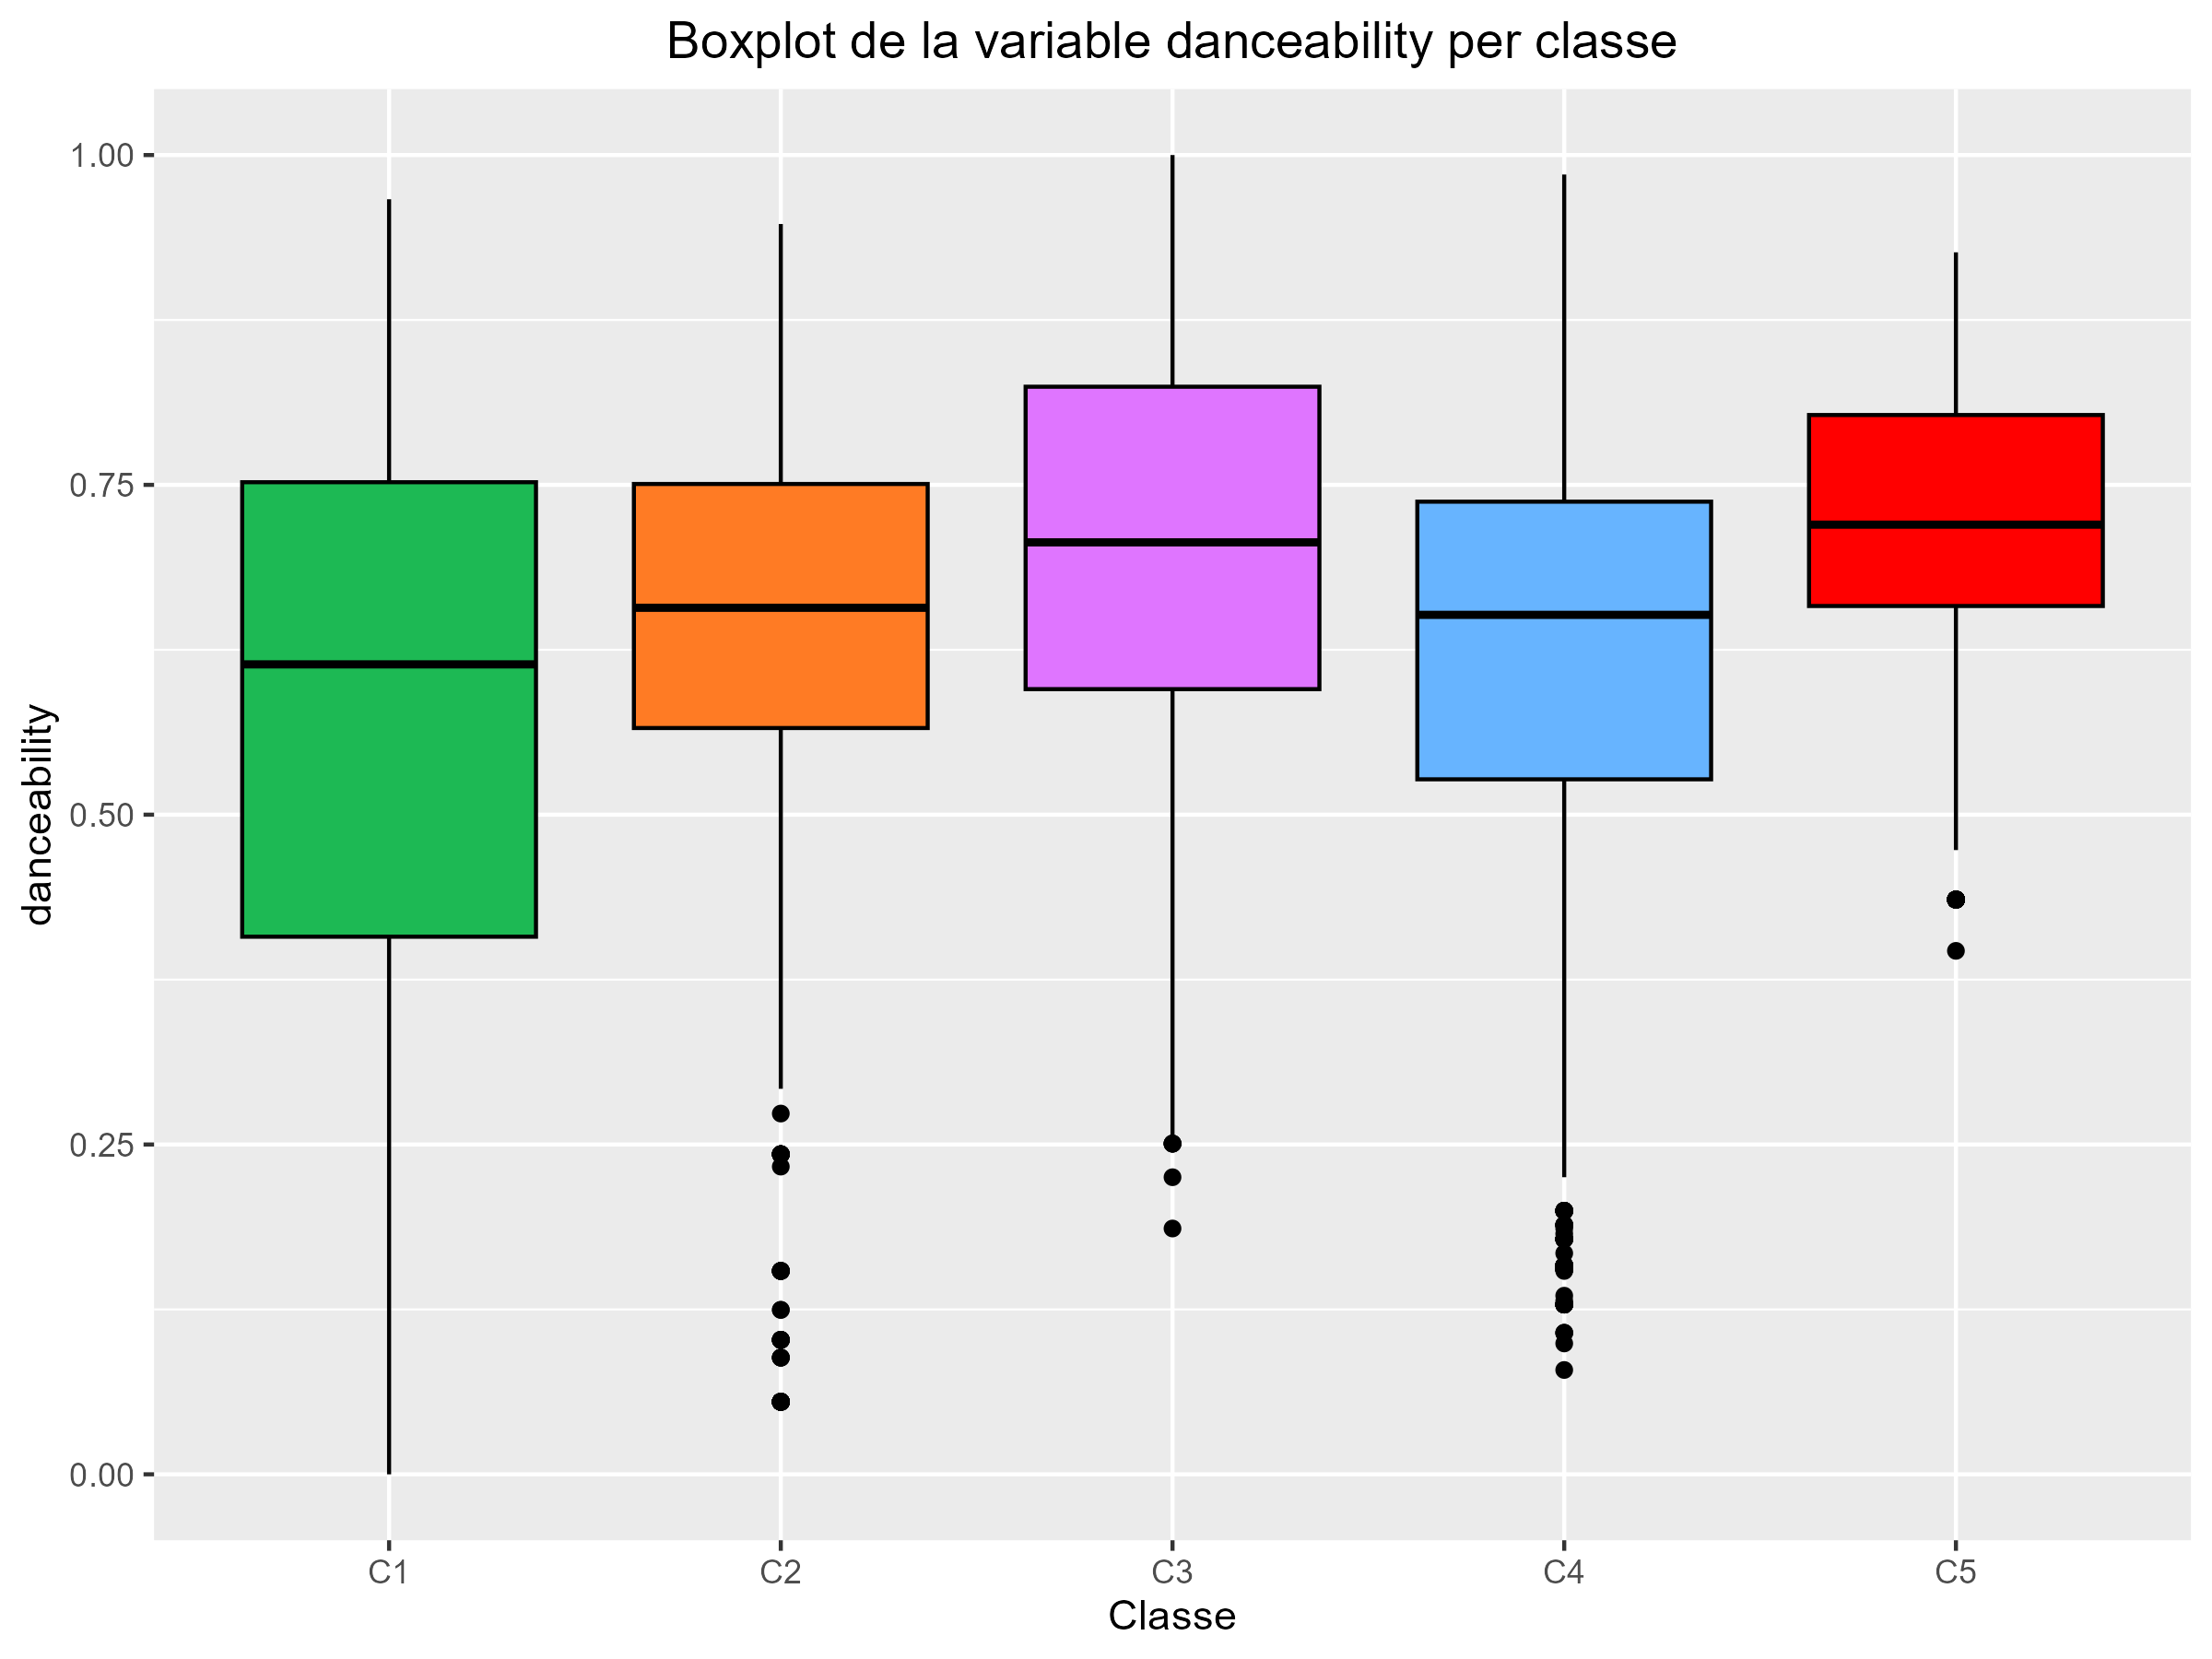
\includegraphics[width=0.95\linewidth]{Images/5_Profiling/numeriques/Num_BoxPlot_danceability.png}
        \caption{Boxplots de danceability per clúster}
        \label{fig:Num_BoxPlot_danceability}
    \end{minipage}%
\end{figure}
En el cas de danceability ens trobem que al primer clúster hi ha les cançons menys ballables en general. En canvi, en els clústers 3 i 5 hi ha cançons que són més ballables que la mitjana. 

\begin{figure}[H]
\centering
    \begin{minipage}{.49\textwidth}
        \centering
        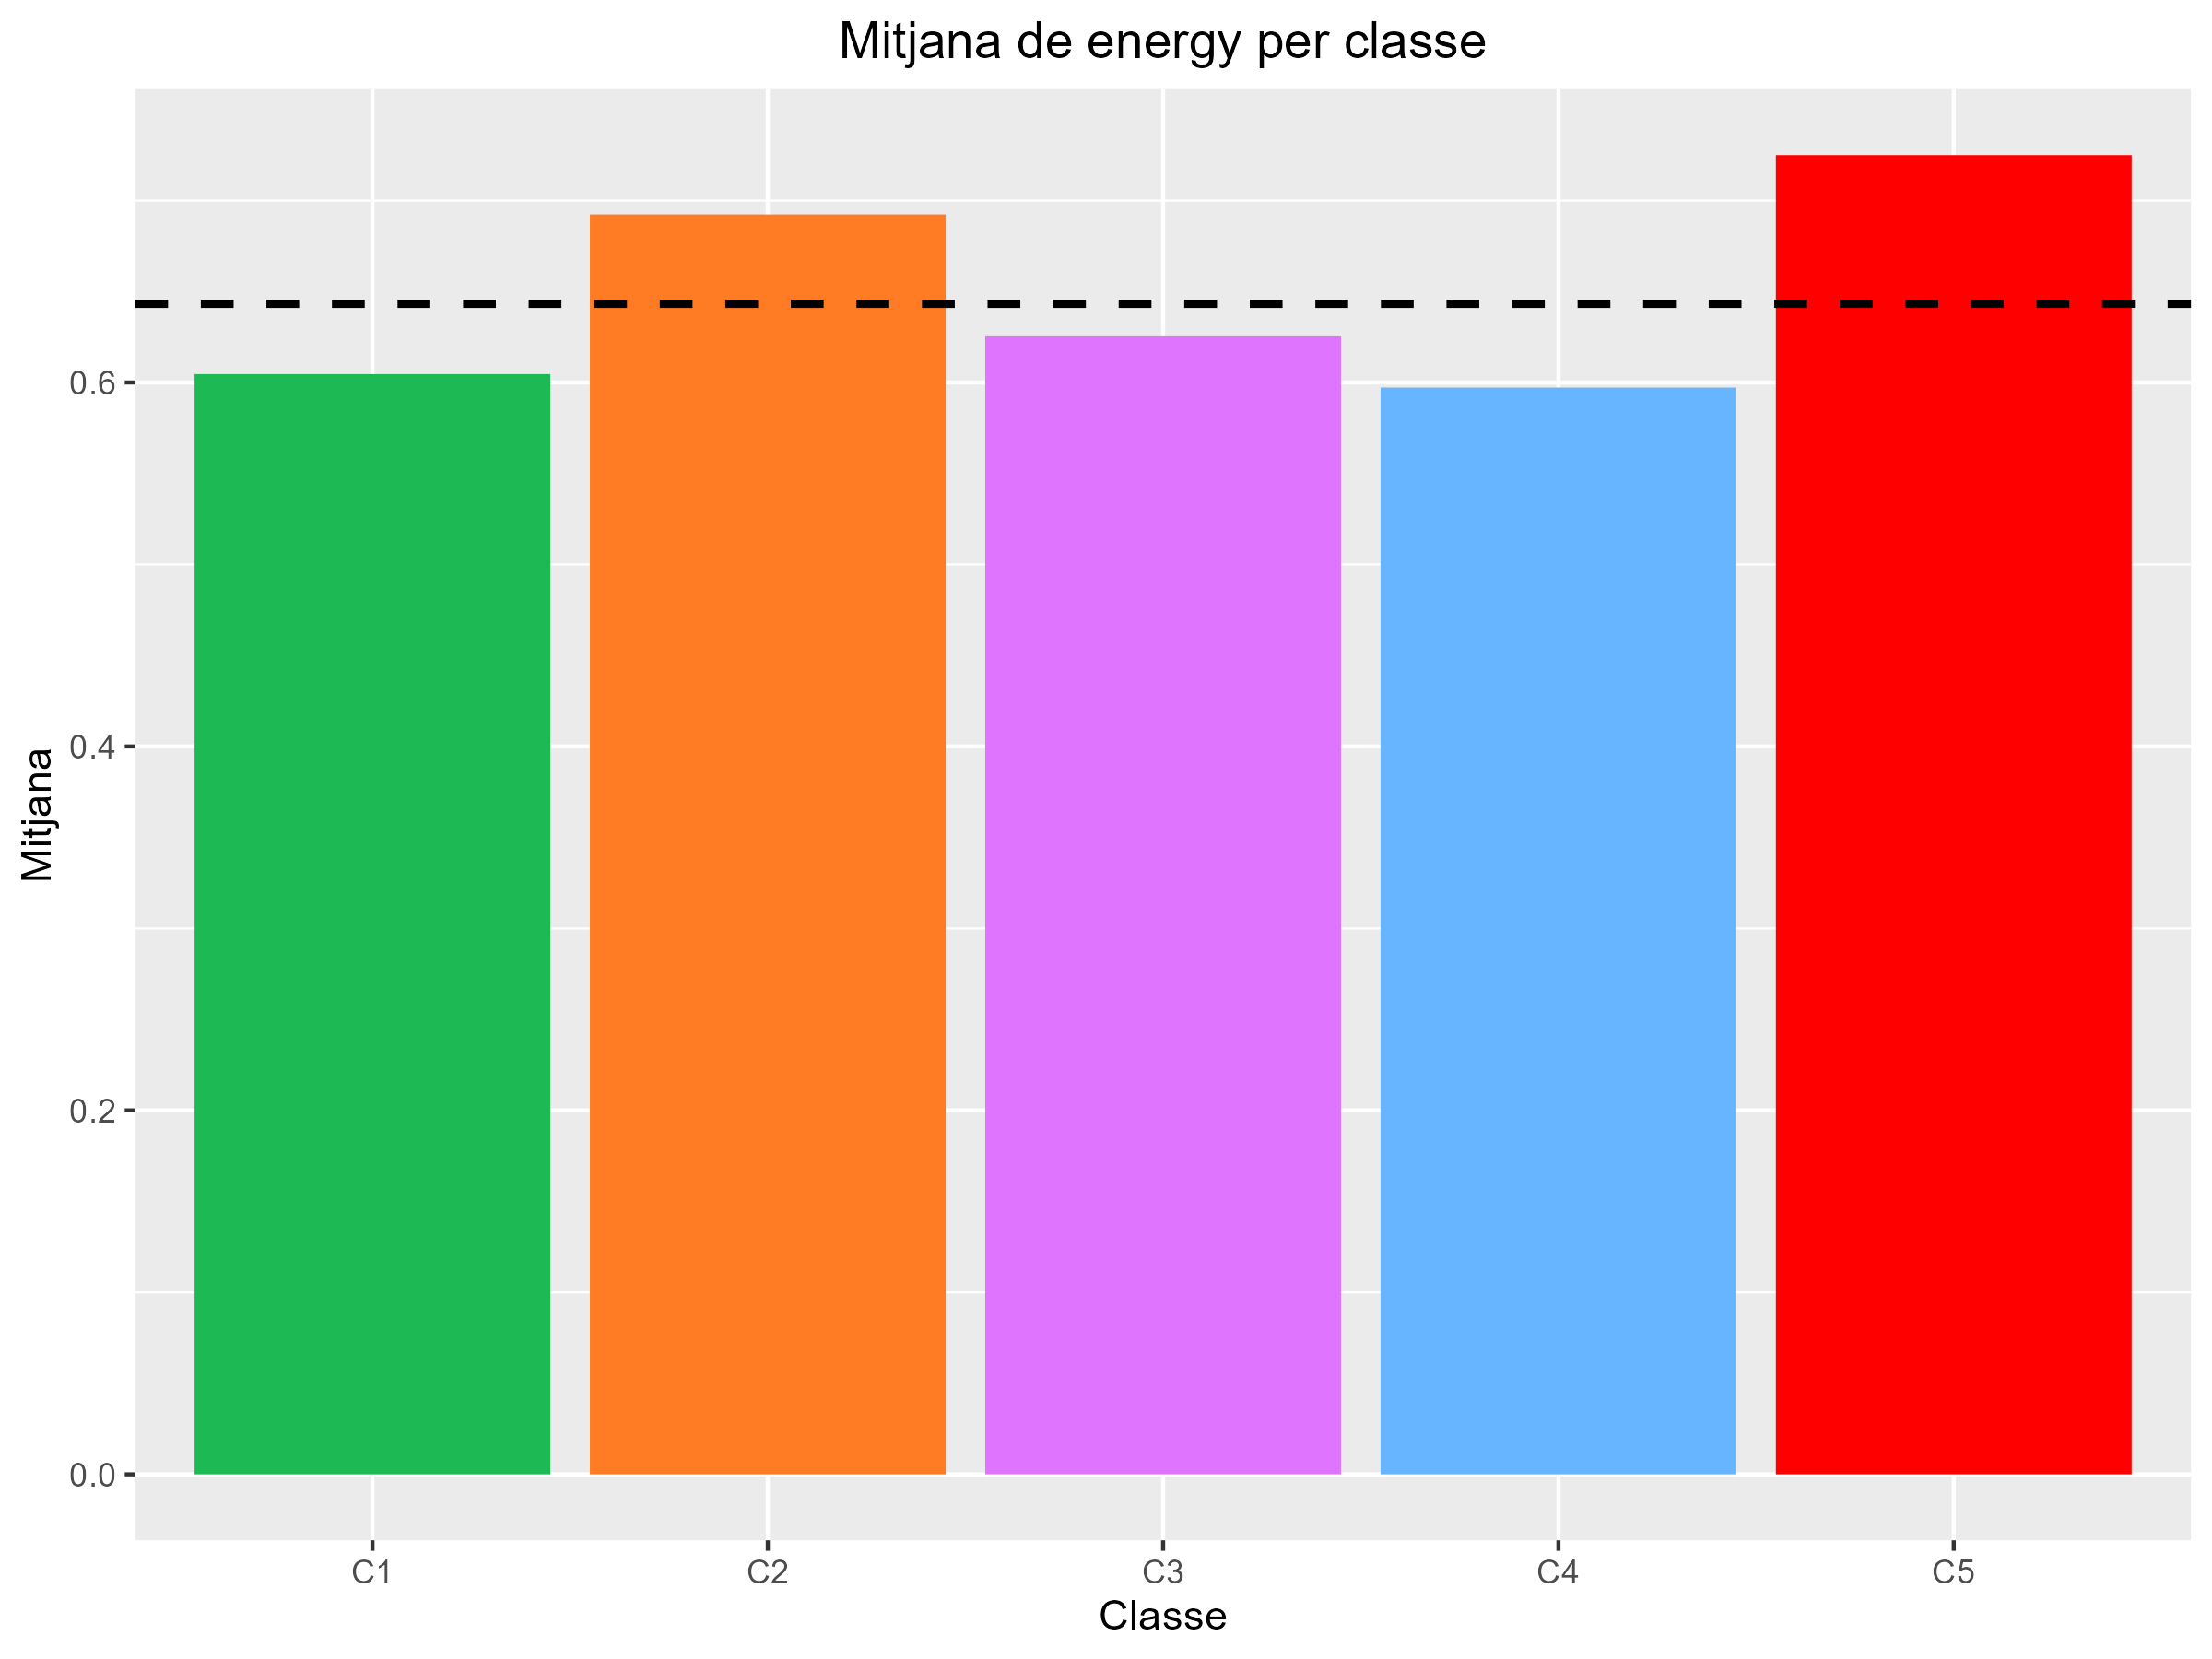
\includegraphics[width=0.95\linewidth]{Images/5_Profiling/numeriques/Num_BarPlot_energy.png}
        \caption{Barplot amb les mitjanes \\ de energy per clúster}
        \label{fig:Num_BarPlot_streams}
    \end{minipage}%
    \begin{minipage}{.49\textwidth}
        \centering
        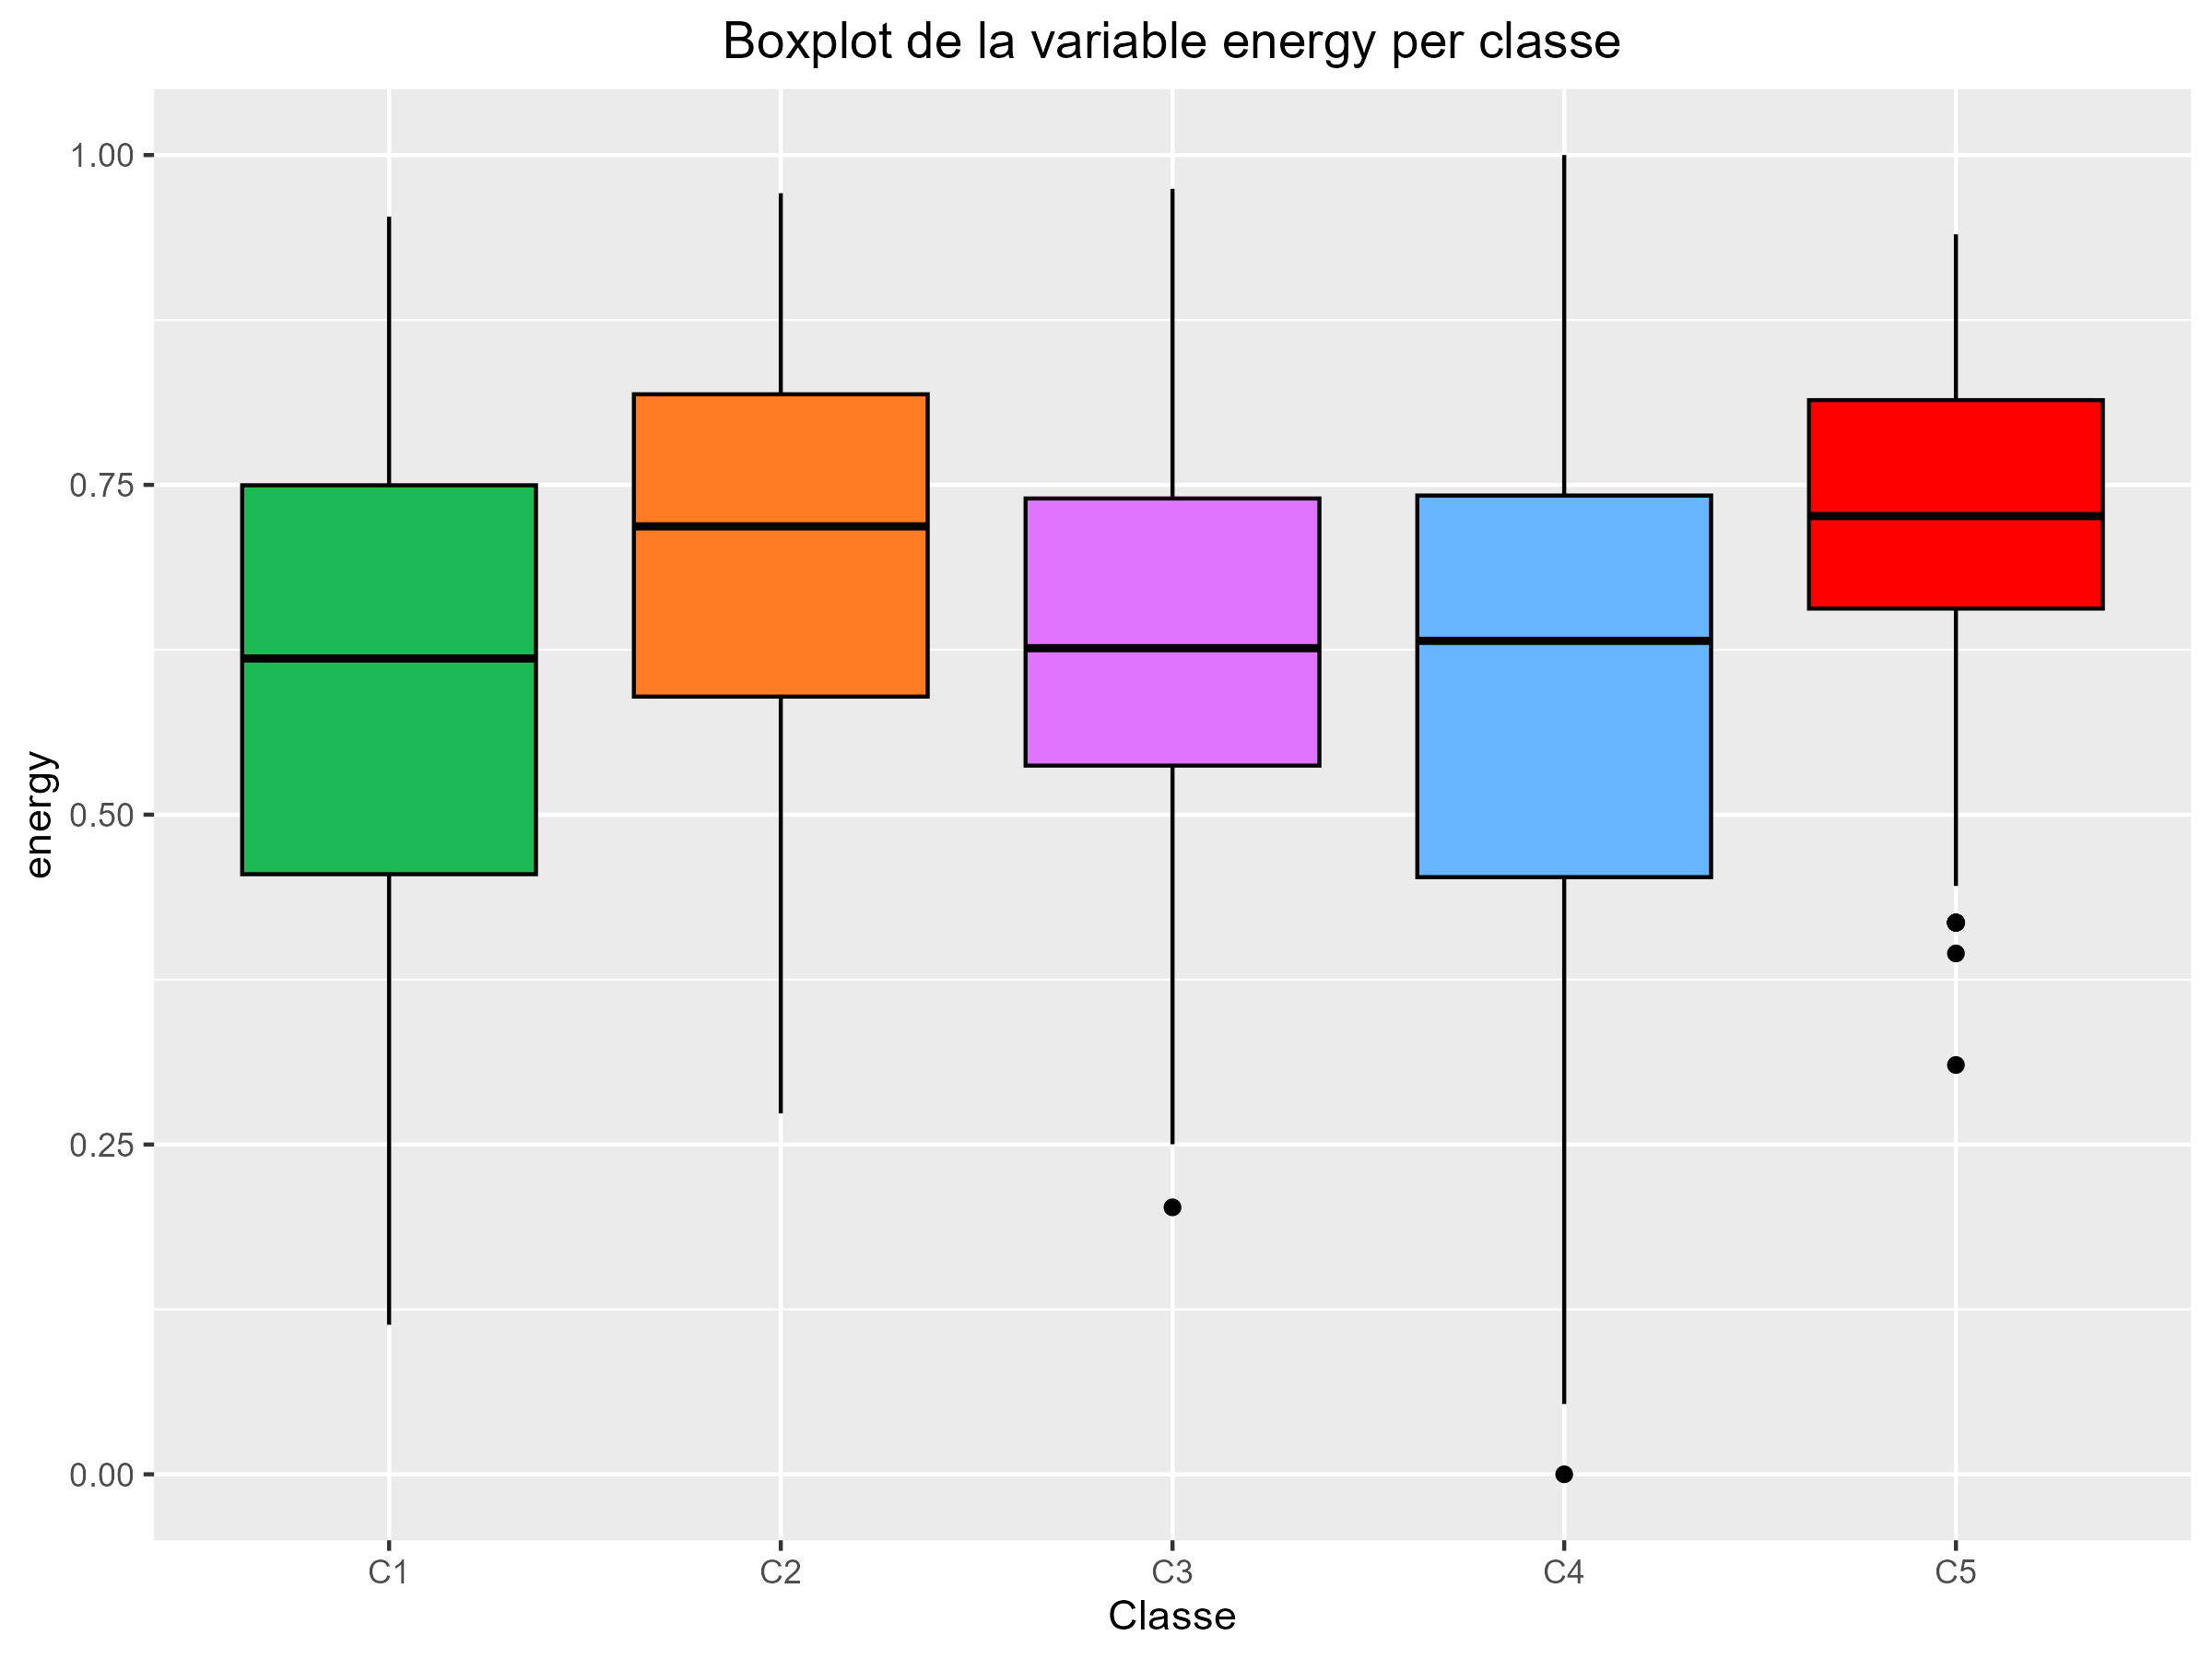
\includegraphics[width=0.95\linewidth]{Images/5_Profiling/numeriques/Num_BoxPlot_energy.png}
        \caption{Boxplots de energy per clúster}
        \label{fig:Num_BoxPlot_streams}
    \end{minipage}%
\end{figure}
En el cas de energy, el clúster 5 conté les cançons que són més energètiques, seguit del 2. Els altres tenen cançons menys energètiques però no molt menys que la mitjana. 
\begin{figure}[H]
\centering
    \begin{minipage}{.49\textwidth}
        \centering
        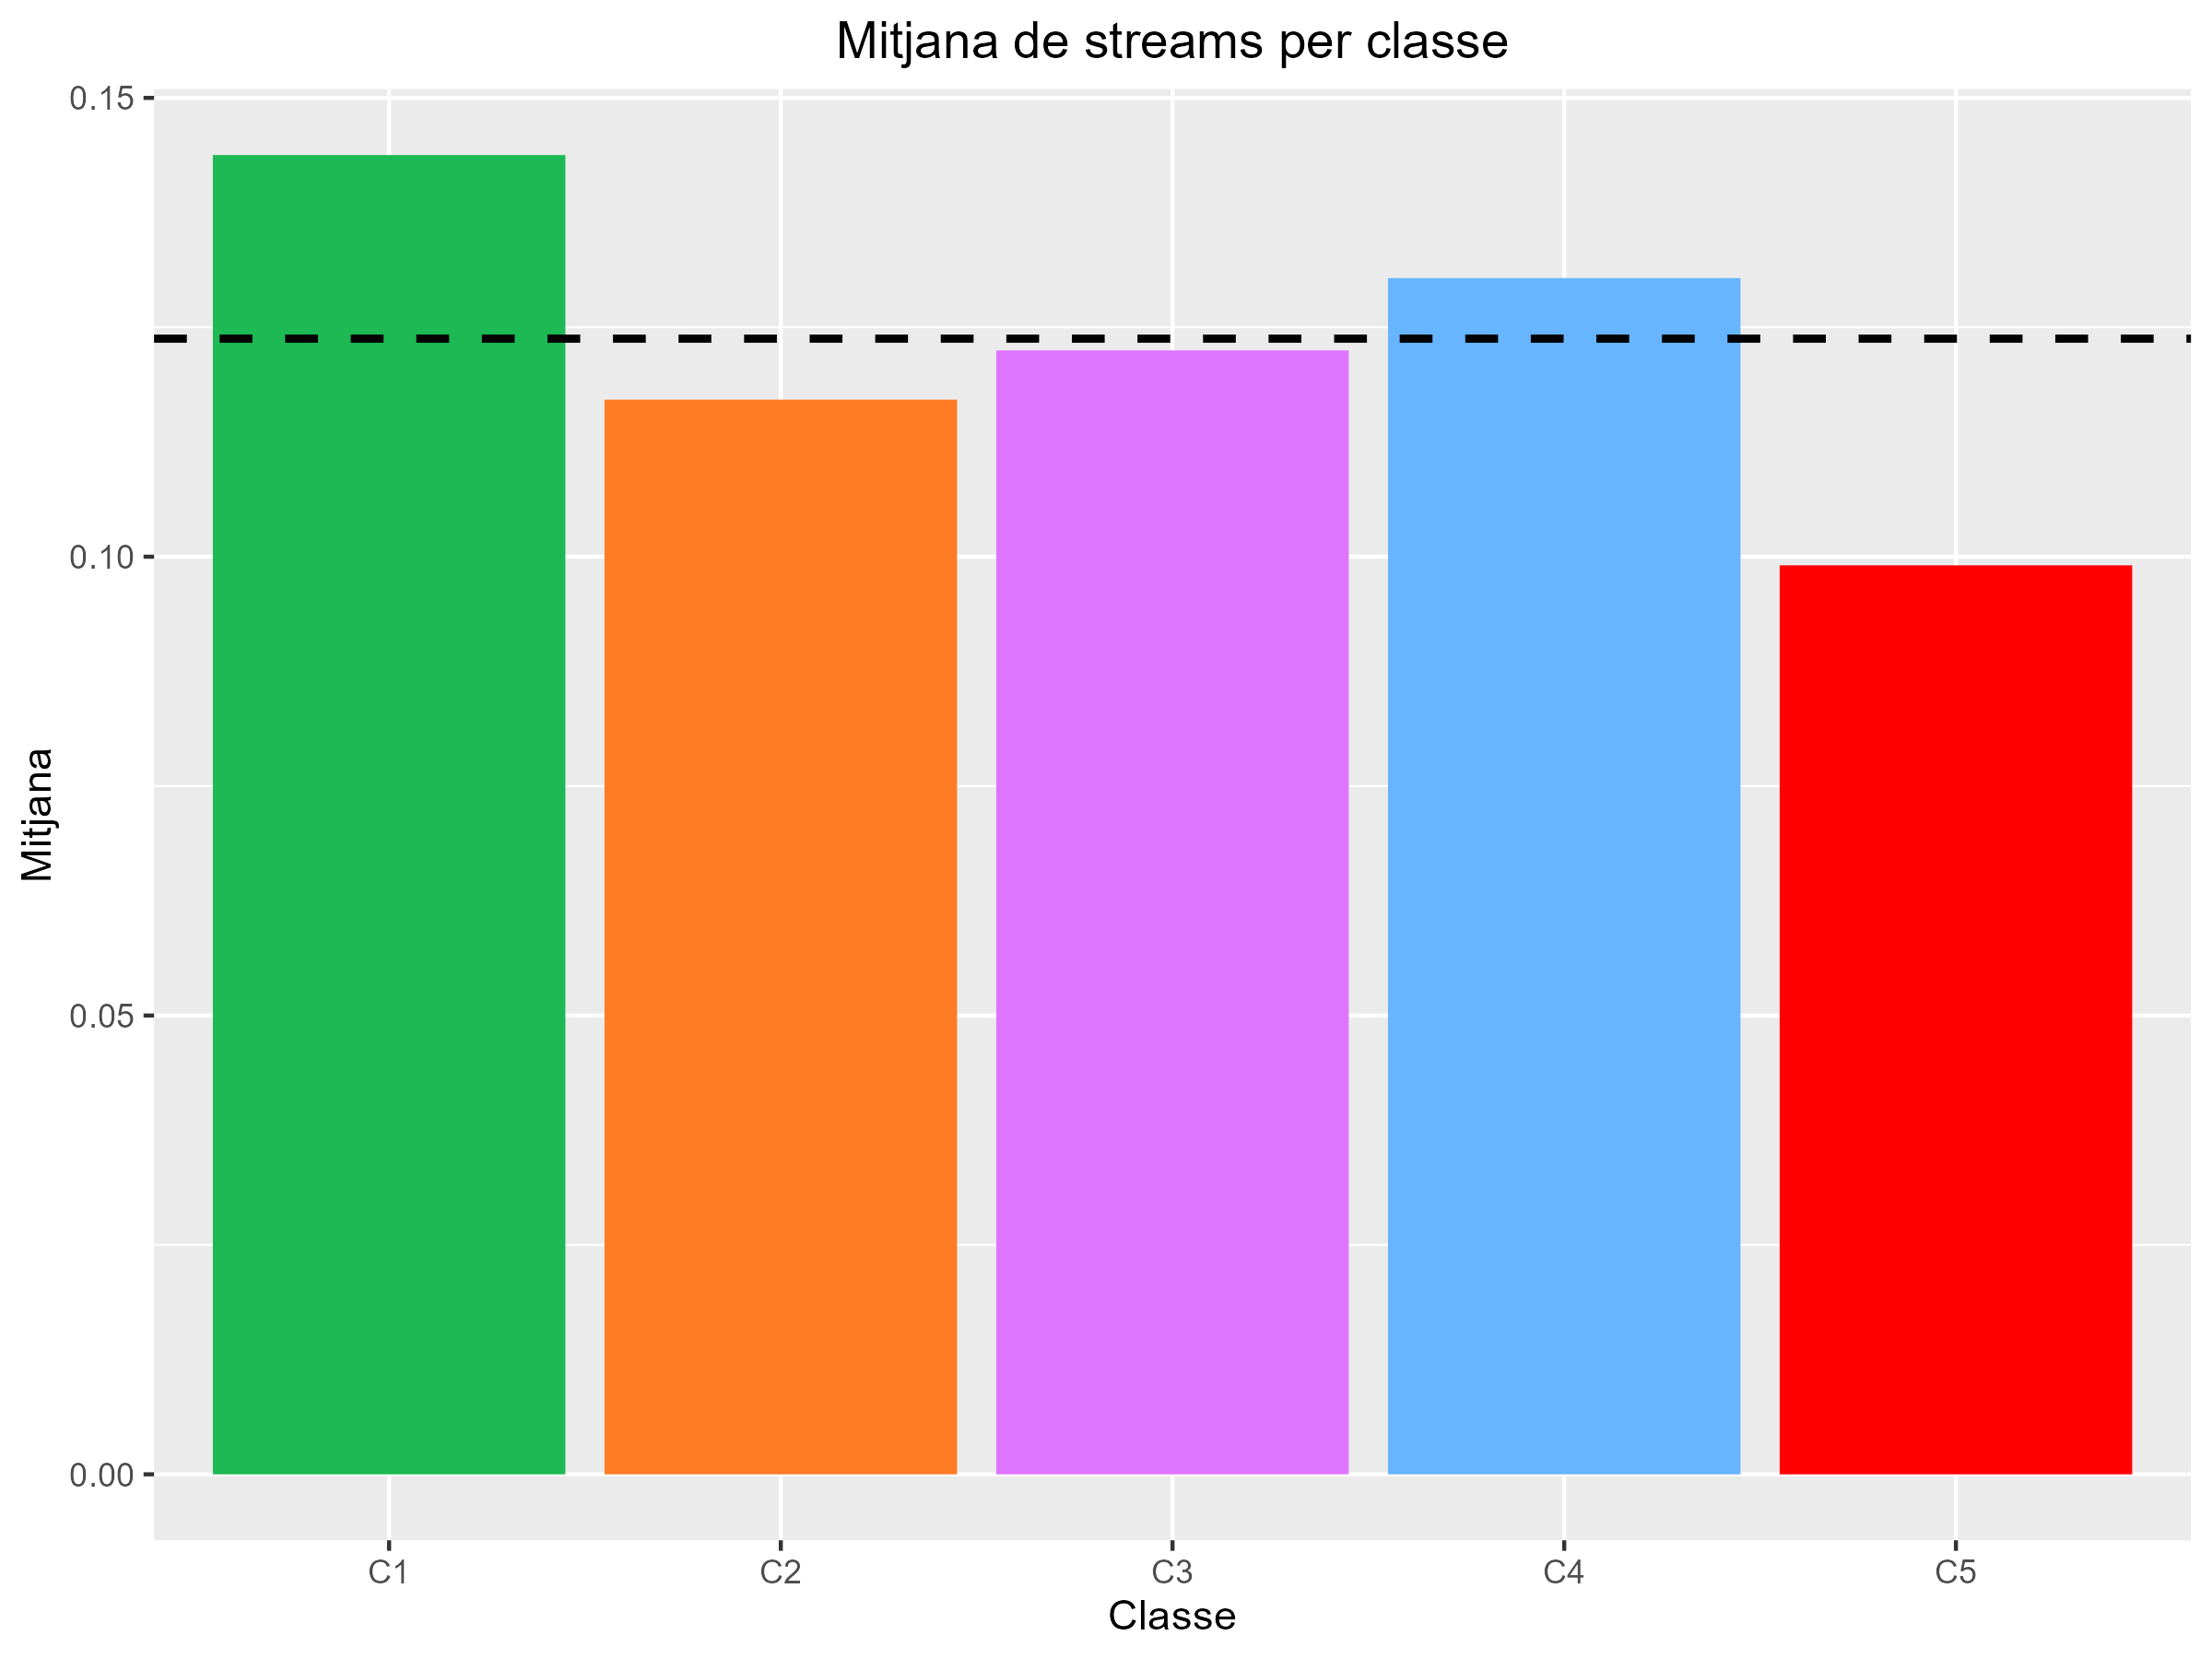
\includegraphics[width=0.95\linewidth]{Images/5_Profiling/numeriques/Num_BarPlot_streams.png}
        \caption{Barplot amb les mitjanes \\ de streams per clúster}
        \label{fig:Num_BarPlot_streams}
    \end{minipage}%
    \begin{minipage}{.49\textwidth}
        \centering
        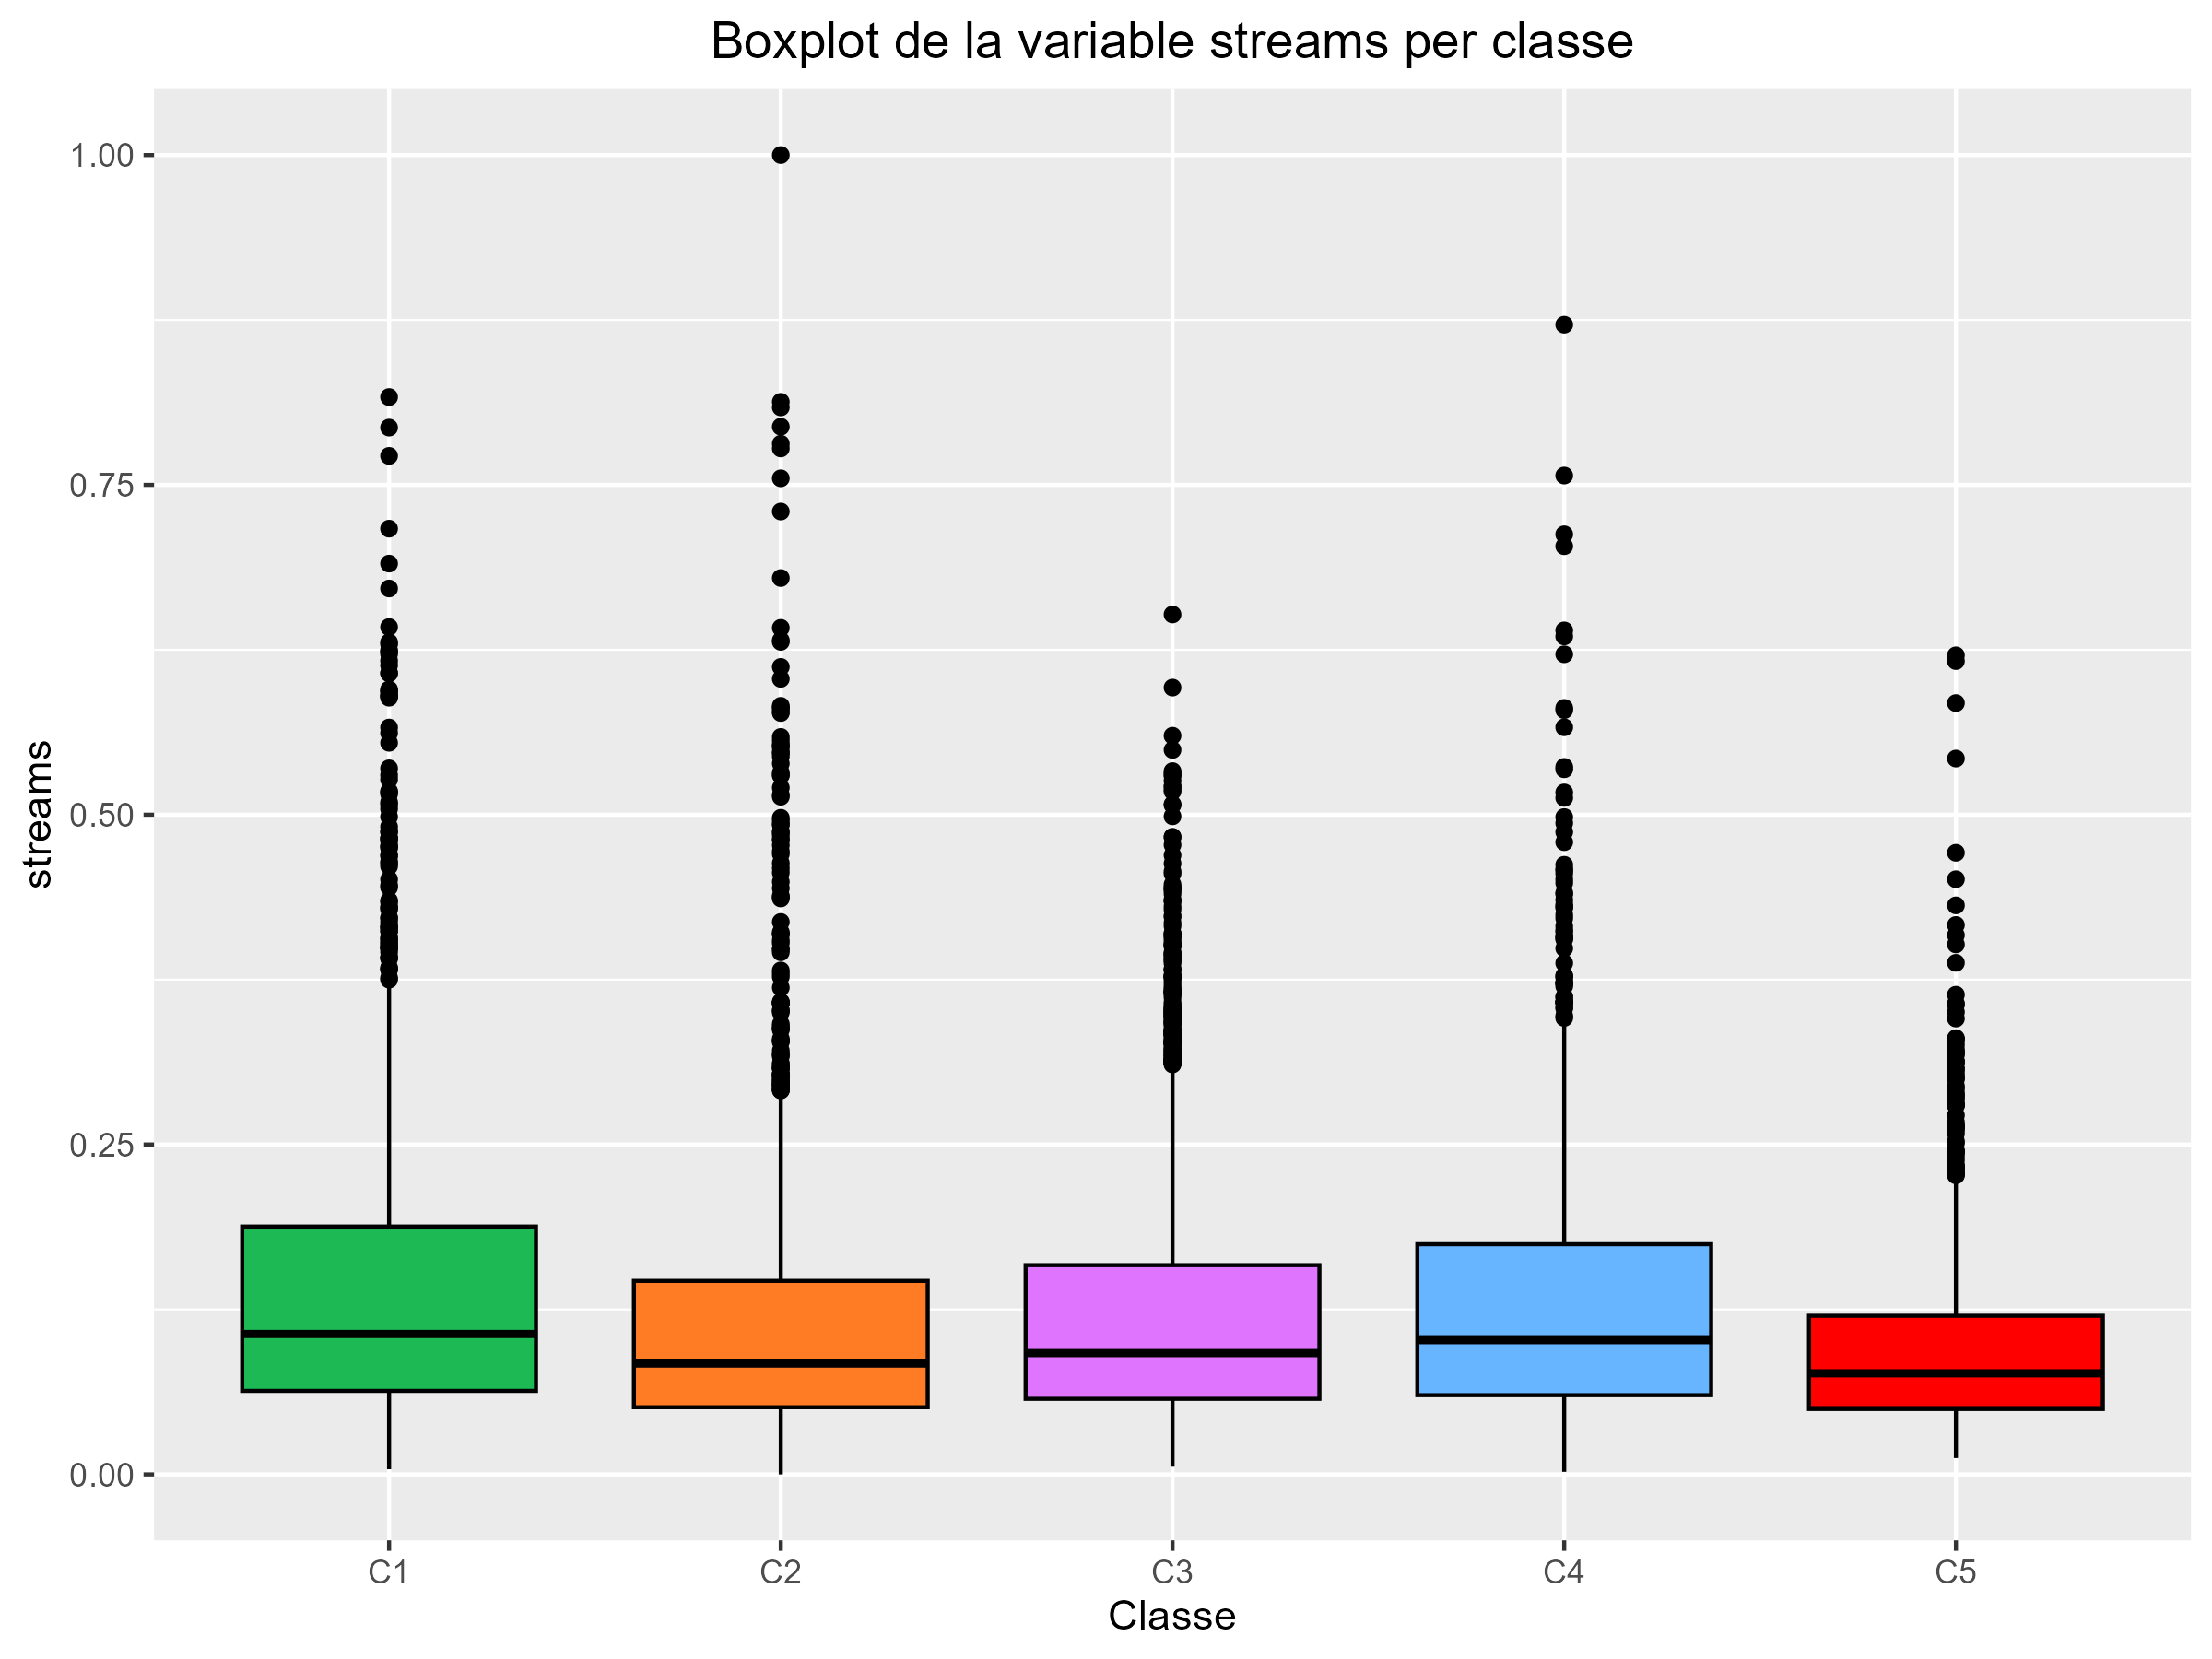
\includegraphics[width=0.95\linewidth]{Images/5_Profiling/numeriques/Num_BoxPlot_streams.png}
        \caption{Boxplots de streams per clúster}
        \label{fig:Num_BoxPlot_streams}
    \end{minipage}%
\end{figure}

A la variable streams ens trobem que la classe 1 té una mitjana relativament alta de streams. També veiem que el cinquè clúster és on hi ha les cançons amb una mitjana més baixa de reproduccions. Tot i això, ja veiem als boxplots que aquestes diferència no són extremadament significatives. 

\begin{figure}[H]
\centering
    \begin{minipage}{.49\textwidth}
        \centering
        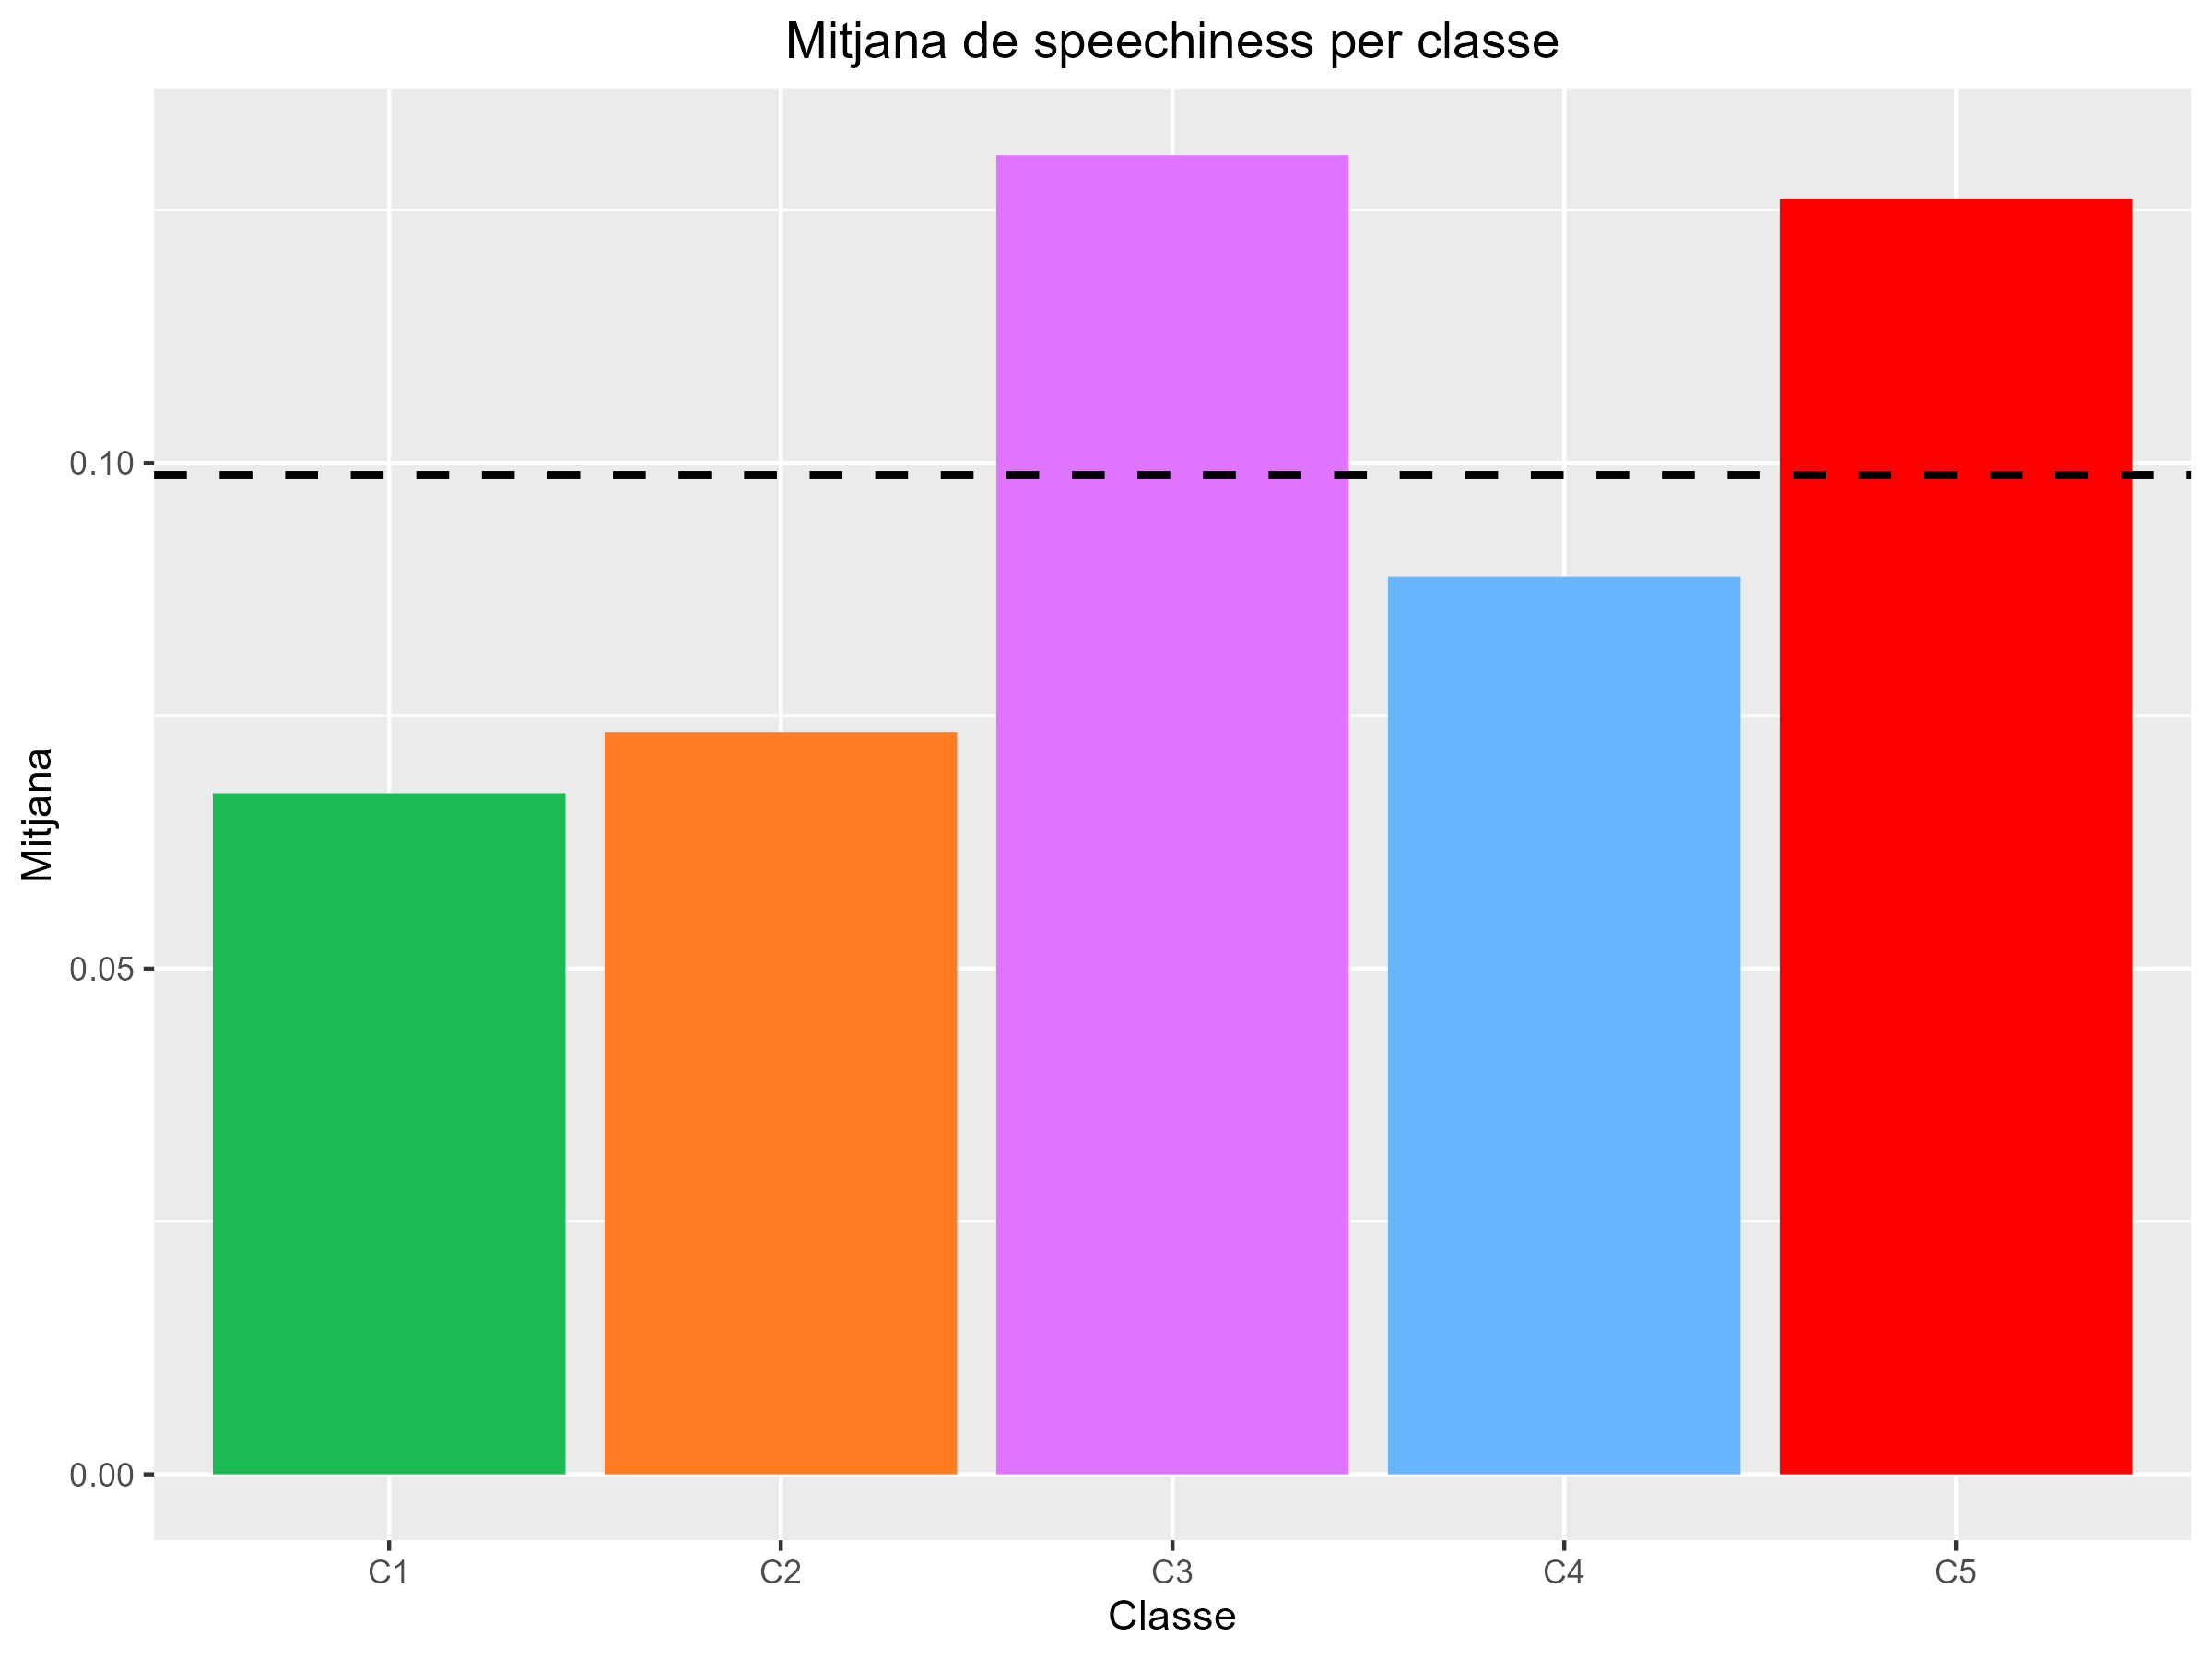
\includegraphics[width=0.95\linewidth]{Images/5_Profiling/numeriques/Num_BarPlot_speechiness.png}
        \caption{Barplot amb les mitjanes \\ de speechiness per clúster}
        \label{fig:Num_BarPlot_speechiness}
    \end{minipage}%
    \begin{minipage}{.49\textwidth}
        \centering
        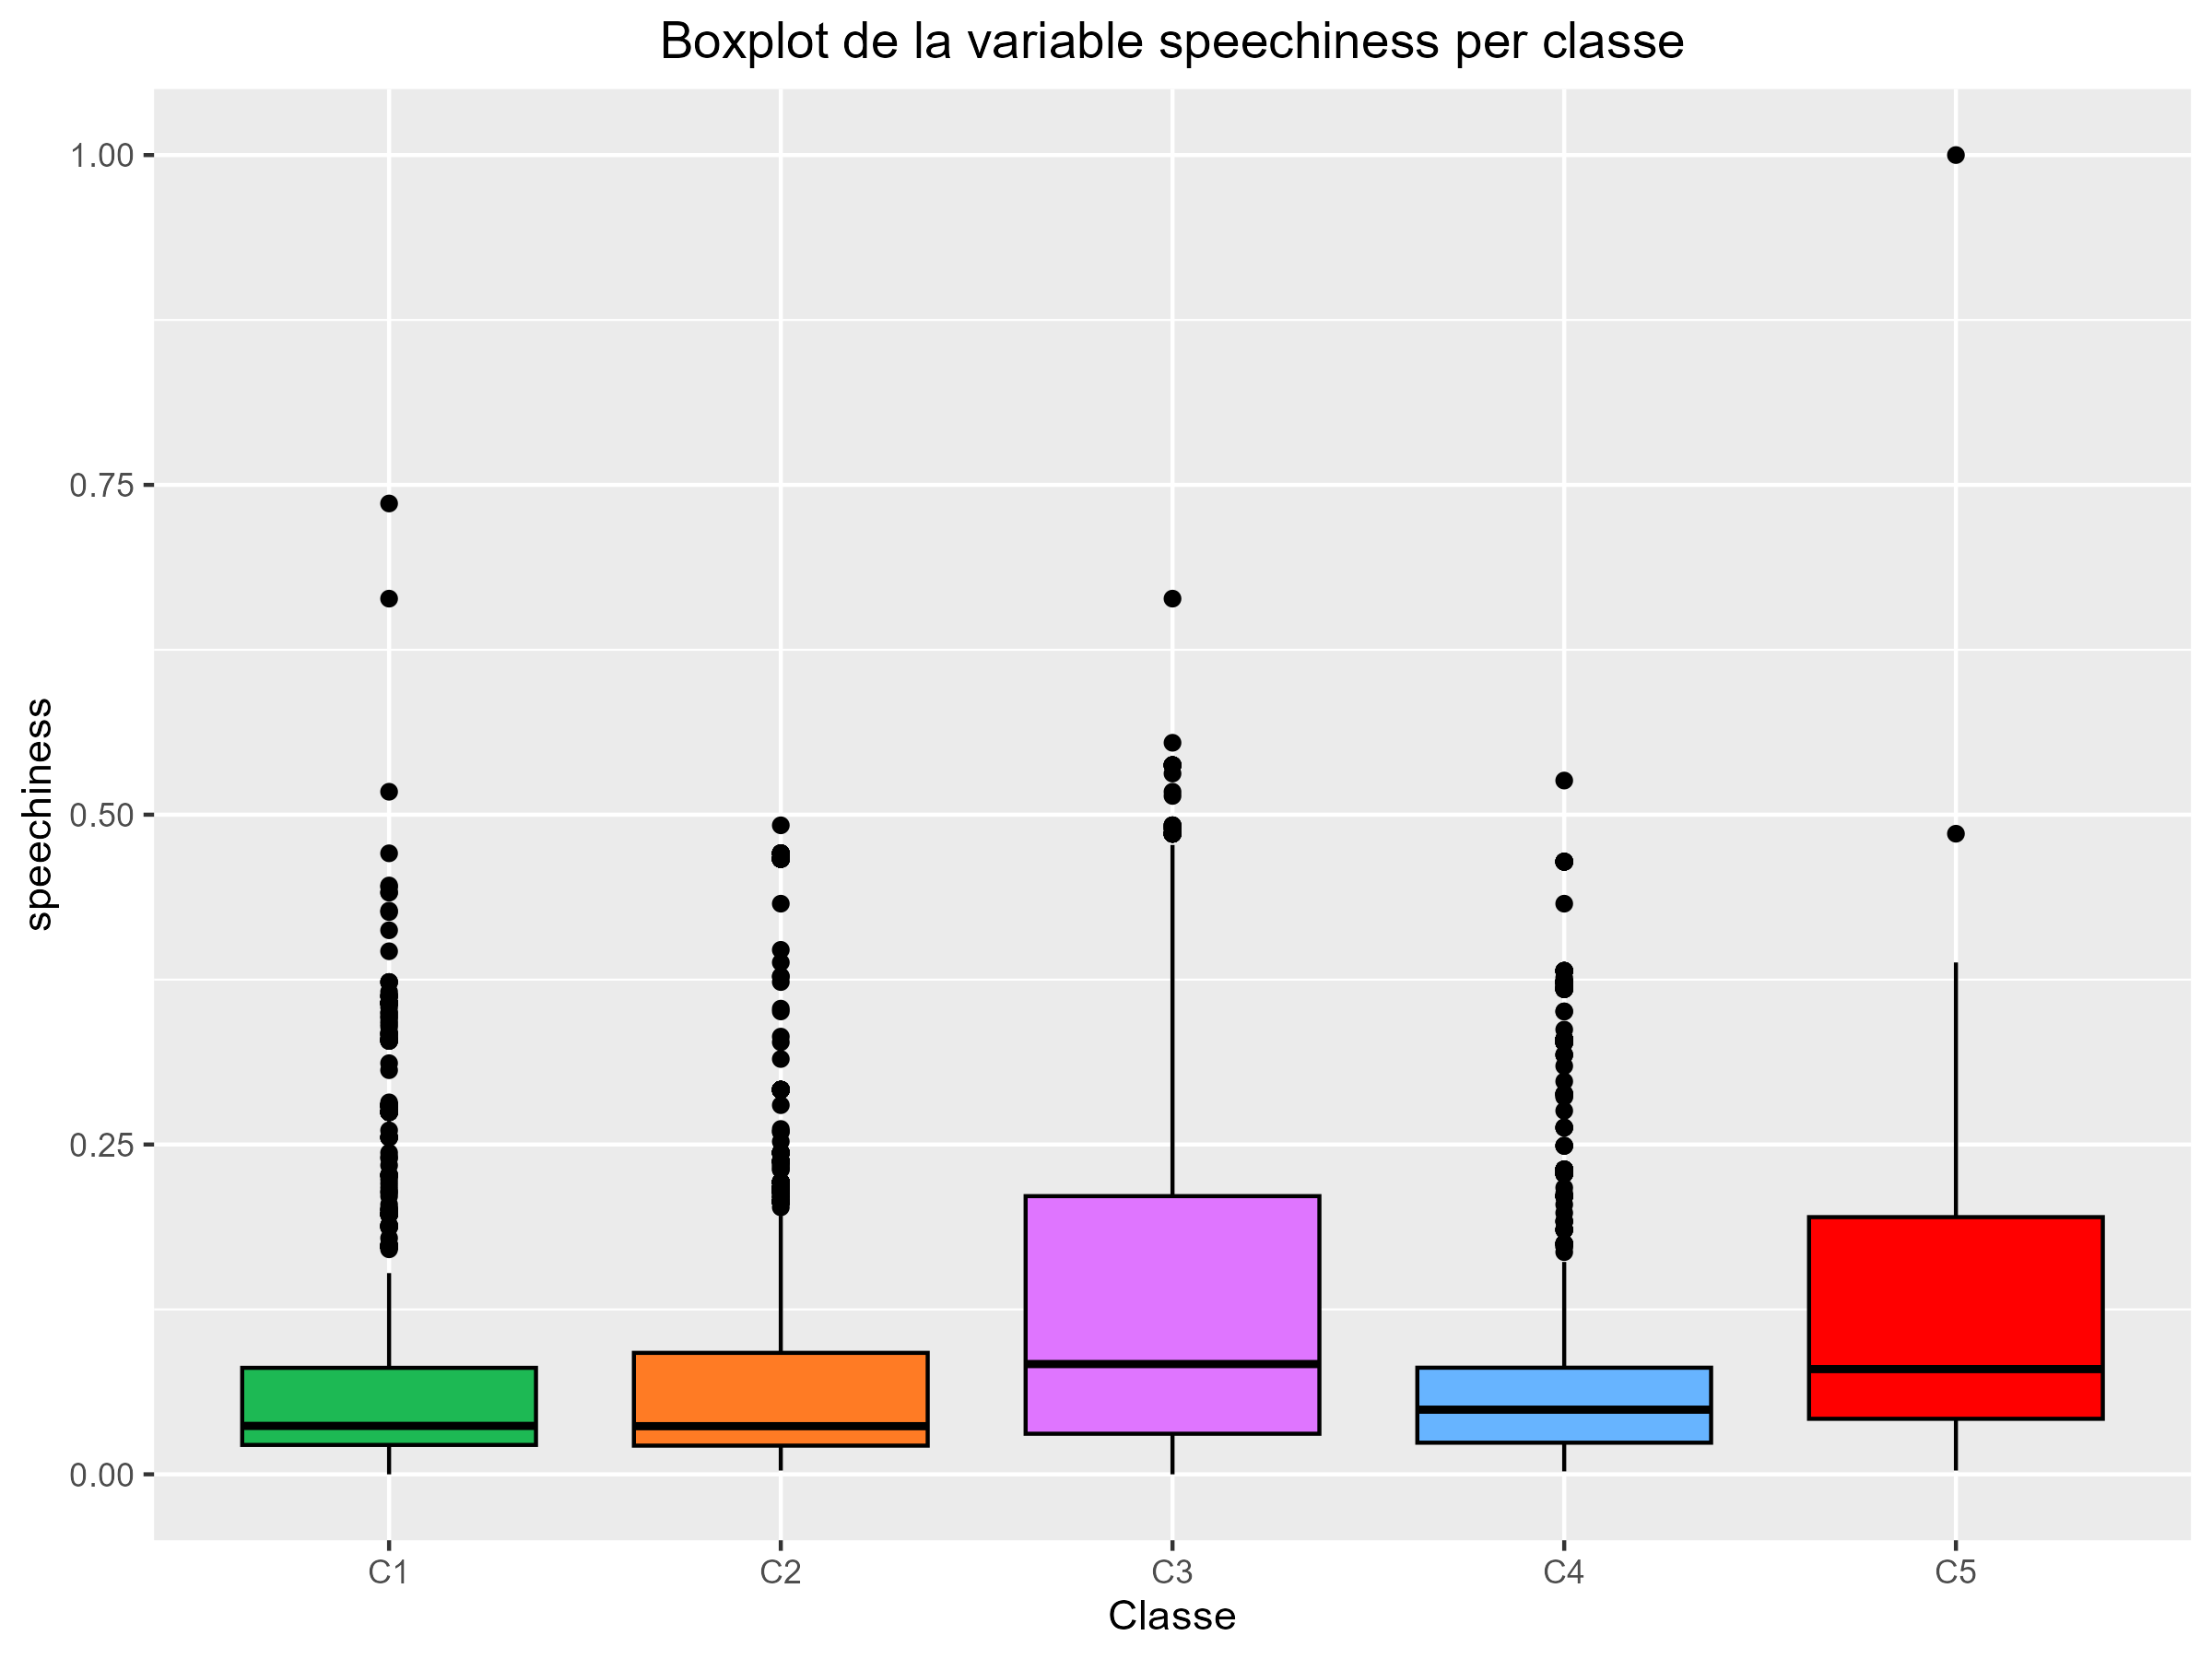
\includegraphics[width=0.95\linewidth]{Images/5_Profiling/numeriques/Num_BoxPlot_speechiness.png}
        \caption{Boxplots de speechiness per clúster}
        \label{fig:Num_BoxPlot_speechiness}
    \end{minipage}%
\end{figure}

Finalment, trobem que la variable speechiness ha influenciat de manera significativa als clústers formats. Amb molta diferència, les mitjanes de les classes 3 i 5 són molt més altes que la mitjana total, i això vol dir que allà es troben les cançons en les que predomina molt més la veu dels artistes. En canvi en els altres clústers, sobretot al primer i al segon, la mitjana és molt més baixa, indicant que allà estan les cançons en les que no hi ha tanta veu. 



\subsection{Variables categòriques}

En quant a les variables categòriques, farem per cada variable el test de chi-quadrat, que compara les distribucions de la variable categòrica amb la columna contenint els valors dels clústers (cada fila de la nostra base de dades a quin clúster pertany). S'avalua si hi ha un associació significativa entre la variable categòrica i els grups dels clústers proporcionant un p-valor.

Comencem a veure les variables que s'han utilitzat pel clustering.

\begin{figure}[H]
\centering
    \begin{minipage}{.49\textwidth}
        \centering
        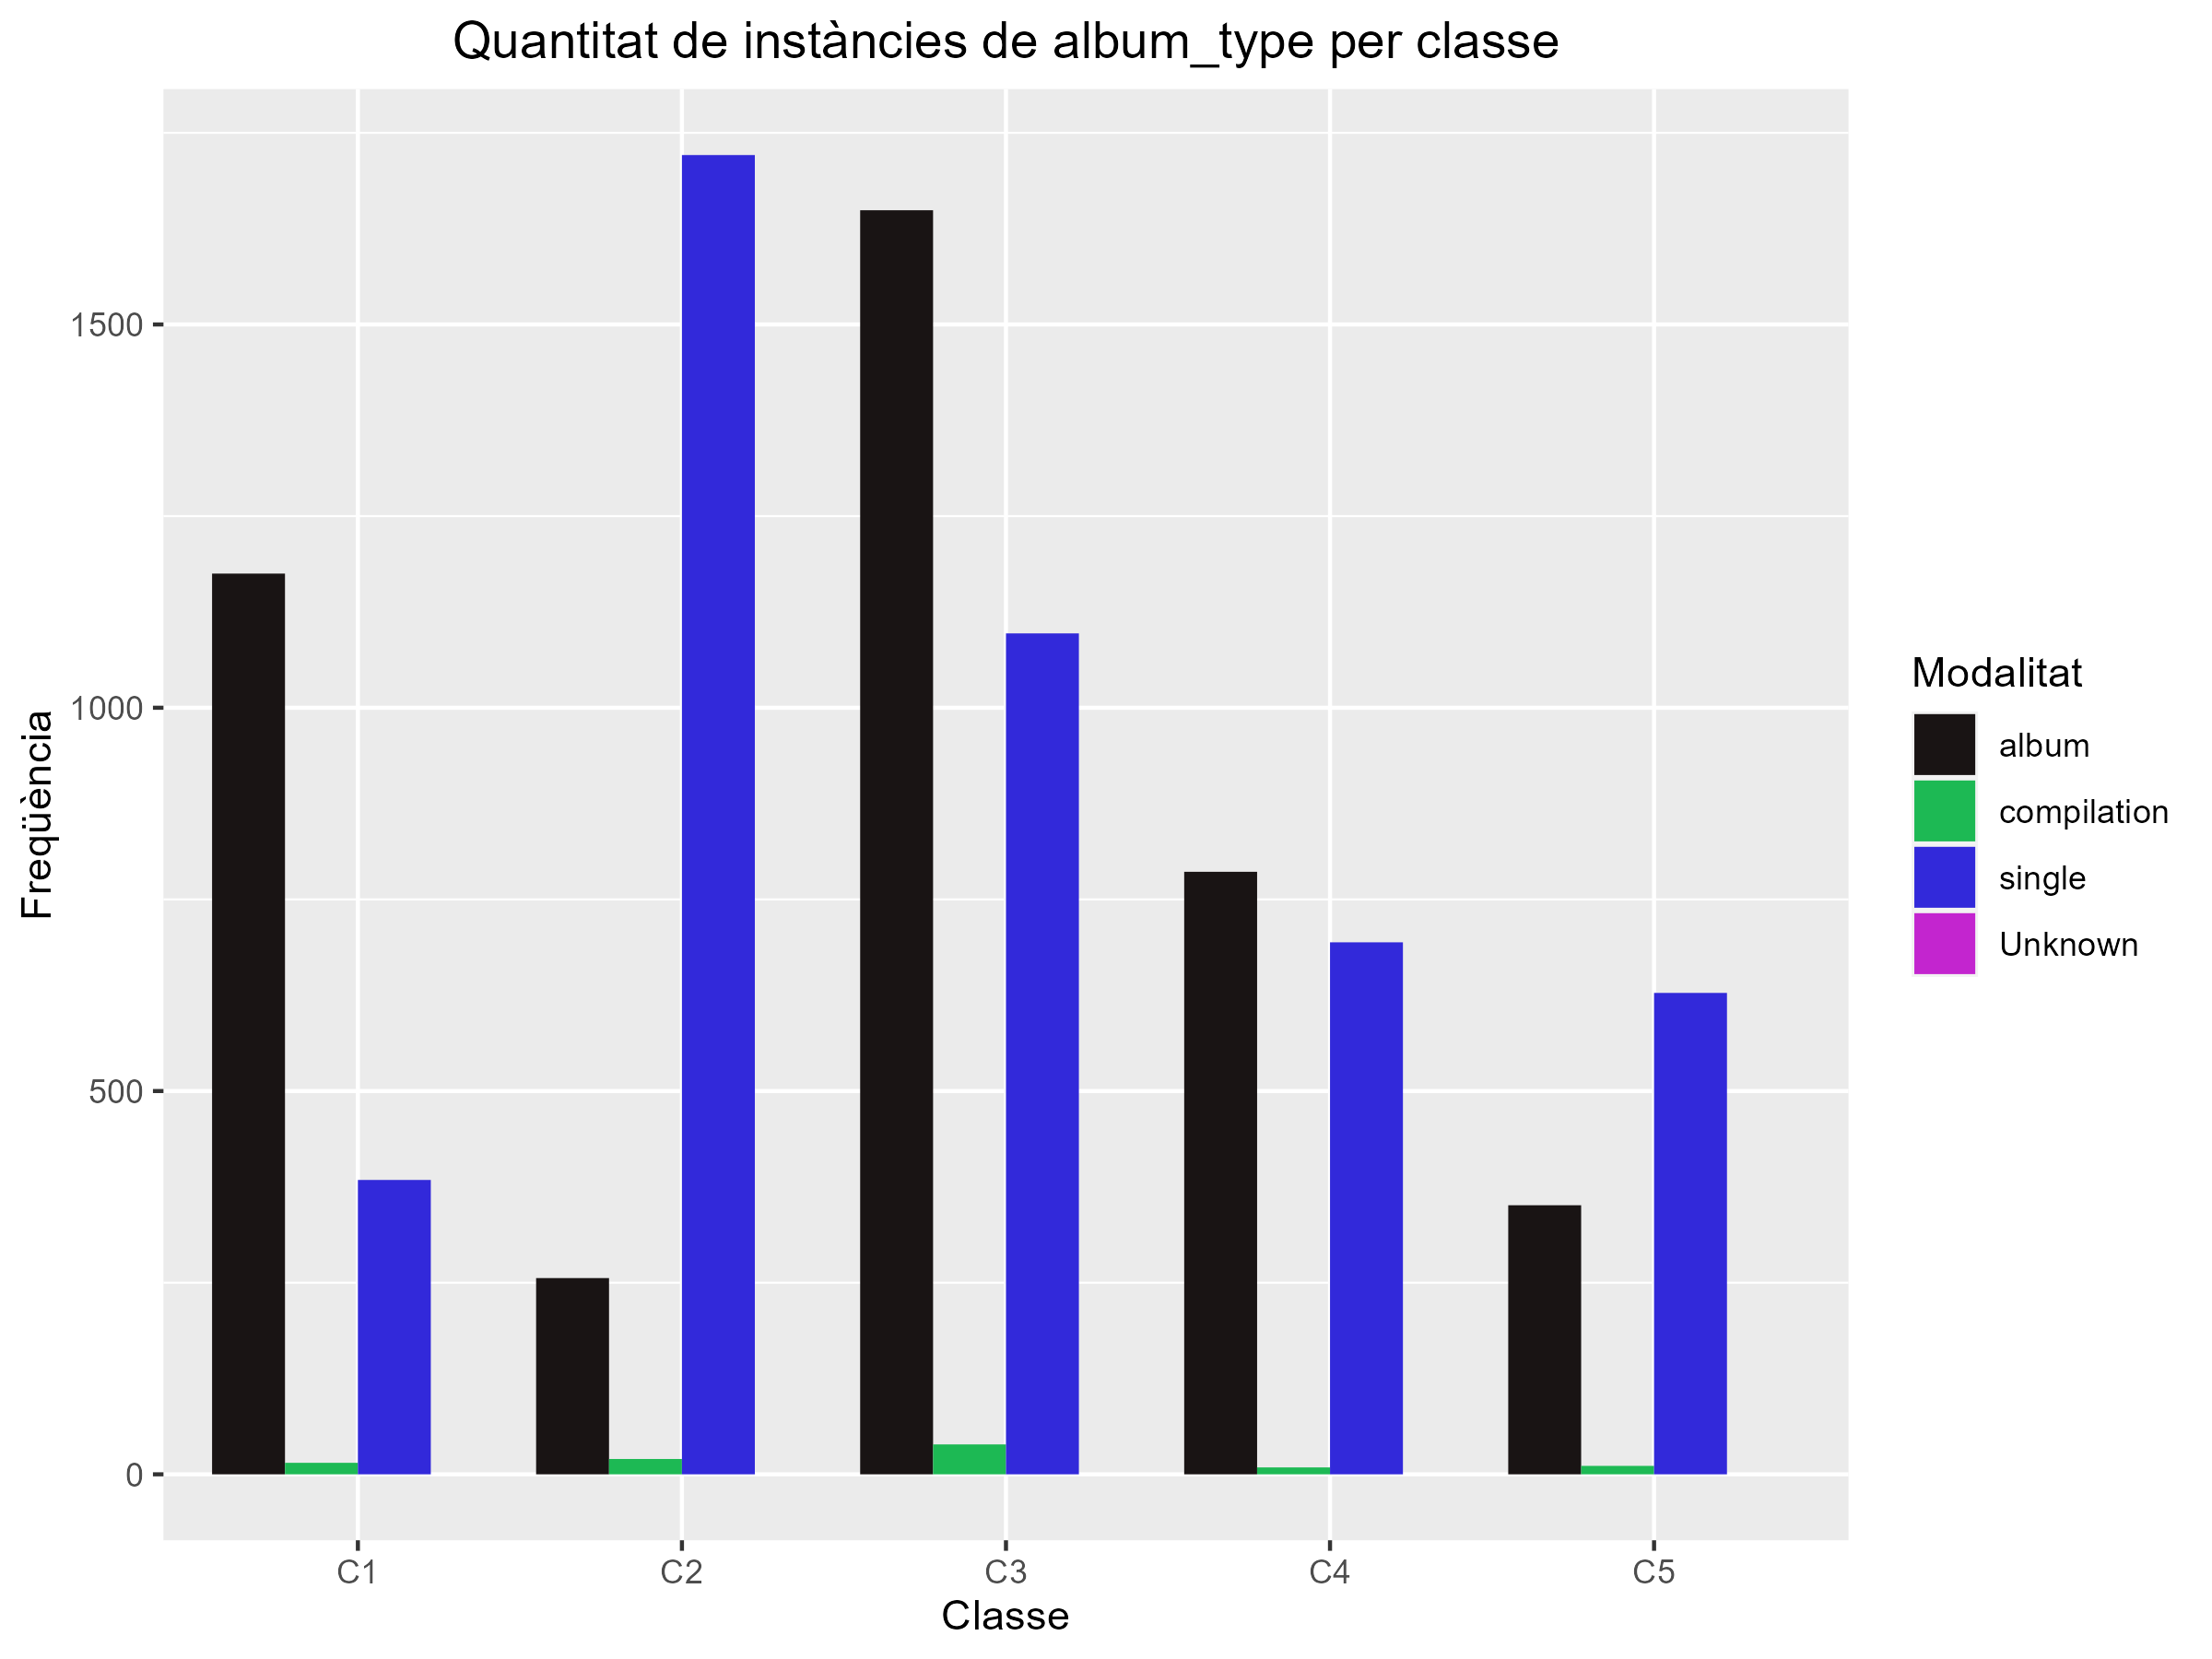
\includegraphics[width=0.95\linewidth]{Images/5_Profiling/categoriques/cat/Cat_BarPlot_album_type.png}
        \caption{Barplot amb els recomptes \\ d'album\_type per clúster}
        \label{fig:Cat_BarPlot_album_type}
    \end{minipage}%
    \begin{minipage}{.49\textwidth}
        \centering
        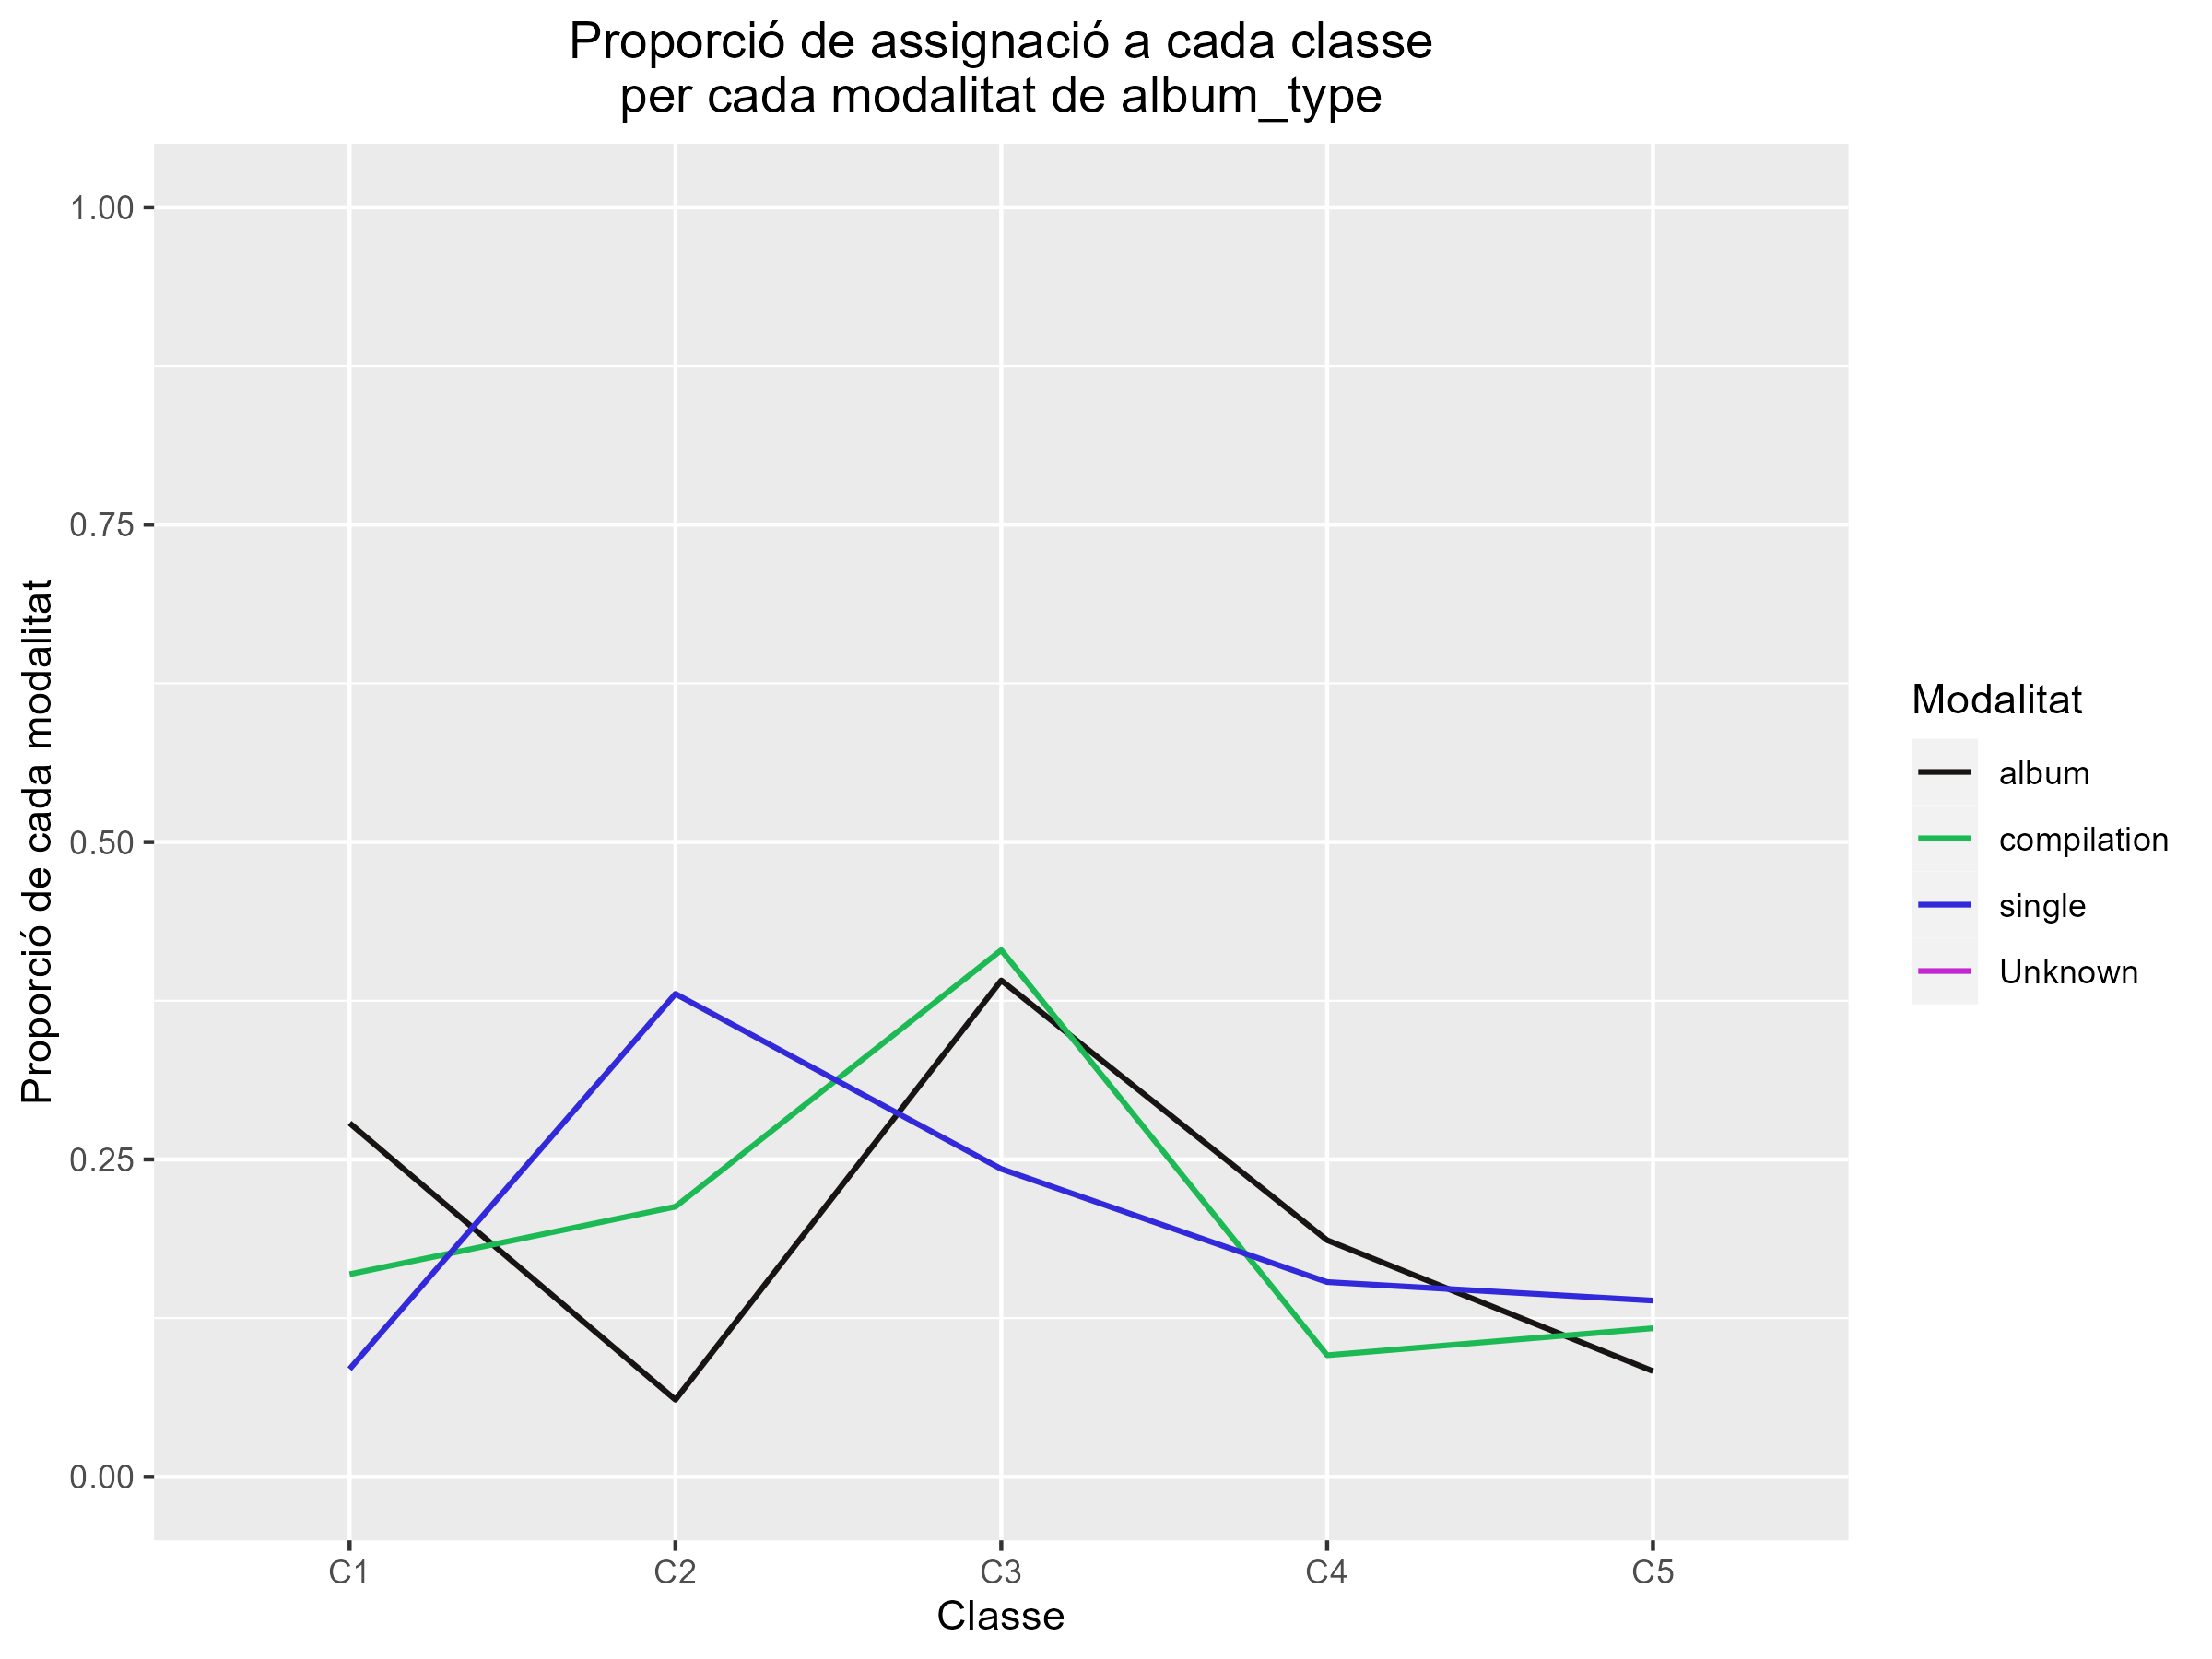
\includegraphics[width=0.95\linewidth]{Images/5_Profiling/categoriques/cat/Cat_SnakePlot_album_type.png}
        \caption{SnakePlot d'album\_type per clúster}
        \label{fig:Cat_SnakePlot_album_type}
    \end{minipage}%
\end{figure}

Com es pot veure als barplots, s'han posat la gran majoria de compilacions i albums a la classe tres. En canvi, al clúster 2 predominen amb molta diferència als singles. A les classes 4 i 5 veiem una proporció semblant de les diferents categories de la variable album\_type. Al clúster 1 també trobem un alt nombre d'instàncies d'album comparades amb les instàncies de single i compilation. Podriem dir que el clúster 3 amb la majoria d'instàncies d'album, podria tenir els valors d'album\_popularity més grans, la qual cosa caldrà seguir comprovant amb més variables. 

\begin{figure}[H]
\centering
    \begin{minipage}{.49\textwidth}
        \centering
        \includegraphics[width=0.95\linewidth]{Images/5_Profiling/categoriques/cat/Cat_BarPlot_christmas.png}
        \caption{Barplot amb els recomptes \\ de christmas per clúster}
        \label{fig:Cat_BarPlot_christmas}
    \end{minipage}%
    \begin{minipage}{.49\textwidth}
        \centering
        \includegraphics[width=0.95\linewidth]{Images/5_Profiling/categoriques/cat/Cat_SnakePlot_christmas.png}
        \caption{SnakePlot de christmas per clúster}
        \label{fig:Cat_SnakePlot_christmas}
    \end{minipage}%
\end{figure}

A la variable christmas, es pot veure que la majoria de les cançons nadalenques es troben al primer clúster. Tot i així també s'observen algunes instàncies al segon clúster. Cal destacar que en el dataset hi ha molt poques instàncies de cançons del gènere christmas, però el fet de que la majoria es concentrin en el clúster 1 ens dona una bona informació sobre aquell clúster. 

%cinema no aporta info

\begin{figure}[H]
\centering
    \begin{minipage}{.49\textwidth}
        \centering
        \includegraphics[width=0.95\linewidth]{Images/5_Profiling/categoriques/cat/Cat_BarPlot_collab.png}
        \caption{Barplot amb els recomptes \\ de collab per clúster}
        \label{fig:Cat_BarPlot_collab}
    \end{minipage}%
    \begin{minipage}{.49\textwidth}
        \centering
        \includegraphics[width=0.95\linewidth]{Images/5_Profiling/categoriques/cat/Cat_SnakePlot_collab.png}
        \caption{SnakePlot de collab per clúster}
        \label{fig:Cat_SnakePlot_collab}
    \end{minipage}%
\end{figure}

A la variable collab, podem obervar que en tots els clústers trobem instàncies tant de cançons amb colaboració com sense. Es pot destacar que als clúster 2 i 5, la majoria d'instàncies són cançons amb colaboració, en canvi els clústers 1 i 4, la majoria de cançons no tenen colaboració. Tot i així, al clúster 3 trobem pràcticament el mateix nombre de cançons amb colaboració i sense.

\begin{figure}[H]
\centering
    \begin{minipage}{.49\textwidth}
        \centering
        \includegraphics[width=0.95\linewidth]{Images/5_Profiling/categoriques/cat/Cat_BarPlot_electro.png}
        \caption{Barplot amb els recomptes \\ de electro per clúster}
        \label{fig:Cat_BarPlot_electro}
    \end{minipage}%
    \begin{minipage}{.49\textwidth}
        \centering
        \includegraphics[width=0.95\linewidth]{Images/5_Profiling/categoriques/cat/Cat_SnakePlot_electro.png}
        \caption{SnakePlot de electro per clúster}
        \label{fig:Cat_SnakePlot_electro}
wa    \end{minipage}%
\end{figure}

A la variable electro, es pot observar que la majoria d'instàncies de les cançons del gènere electro es troben en els clústers 2 i 4. En canvi, els clústers 1 i 3 no contenen pràcticament instàncies d'aquest gènere, a més, el clúster 5 no conté cap instància del gènere electro.

\begin{figure}[H]
\centering
    \begin{minipage}{.49\textwidth}
        \centering
        \includegraphics[width=0.95\linewidth]{Images/5_Profiling/categoriques/cat/Cat_BarPlot_explicit.png}
        \caption{Barplot amb els recomptes \\ de explicit per clúster}
        \label{fig:Cat_BarPlot_explicit}
    \end{minipage}%
    \begin{minipage}{.49\textwidth}
        \centering
        \includegraphics[width=0.95\linewidth]{Images/5_Profiling/categoriques/cat/Cat_SnakePlot_explicit.png}
        \caption{SnakePlot de explicit per clúster}
        \label{fig:Cat_SnakePlot_explicit}
    \end{minipage}%
\end{figure}

A la variable explicit, trobem que la gran majoria de cançons explícites es troben al tercer clúster. Tot i així, els altres clústers també tenen instàncies de cançons explícites, encara que contenen moltes més instàncies de cançons no explícites que d'explícites.

\begin{figure}[H]
\centering
    \begin{minipage}{.49\textwidth}
        \centering
        \includegraphics[width=0.95\linewidth]{Images/5_Profiling/categoriques/cat/Cat_BarPlot_hip_hop.png}
        \caption{Barplot amb els recomptes \\ de hip-hop per clúster}
        \label{fig:Cat_BarPlot_hip_hop}
    \end{minipage}%
    \begin{minipage}{.49\textwidth}
        \centering
        \includegraphics[width=0.95\linewidth]{Images/5_Profiling/categoriques/cat/Cat_SnakePlot_hip_hop.png}
        \caption{SnakePlot de hip-hop per clúster}
        \label{fig:Cat_SnakePlot_hip_hop}
    \end{minipage}%
\end{figure}

A la variable hip\_hop trobem que la majoria d'instàncies es troben en el tercer clúster, tot i així, al cinquè clúster també trobem gran part d'aquestes. En canvi, als altres clústers pràcticament no trobem cap cançó del gènere hip hop.

\begin{figure}[H]
\centering
    \begin{minipage}{.49\textwidth}
        \centering
        \includegraphics[width=0.95\linewidth]{Images/5_Profiling/categoriques/cat/Cat_BarPlot_latino.png}
        \caption{Barplot amb els recomptes \\ de latino per clúster}
        \label{fig:Cat_BarPlot_latino}
    \end{minipage}%
    \begin{minipage}{.49\textwidth}
        \centering
        \includegraphics[width=0.95\linewidth]{Images/5_Profiling/categoriques/cat/Cat_SnakePlot_latino.png}
        \caption{SnakePlot de latino per clúster}
        \label{fig:Cat_SnakePlot_latino}
    \end{minipage}%
\end{figure}

A la variable latino, es pot observar que pràcticament el 90\% de les cançons de gènere latino es troben en el cinquè clúster. Mentre que a la resta de clústers no trobem pràcticament cançons d'aquest gènere.

\begin{figure}[H]
\centering
    \begin{minipage}{.49\textwidth}
        \centering
        \includegraphics[width=0.95\linewidth]{Images/5_Profiling/categoriques/cat/Cat_BarPlot_rock.png}
        \caption{Barplot amb els recomptes \\ de rock per clúster}
        \label{fig:Cat_BarPlot_rock}
    \end{minipage}%
    \begin{minipage}{.49\textwidth}
        \centering
        \includegraphics[width=0.95\linewidth]{Images/5_Profiling/categoriques/cat/Cat_SnakePlot_rock.png}
        \caption{SnakePlot de rock per clúster}
        \label{fig:Cat_SnakePlot_rock}
    \end{minipage}%
\end{figure}

A la variable rock, es pot observar que més del 90\% de les cançons de gènere rock es troben en el primer clúster. Mentre que a la resta de clústers no trobem pràcticament cançons d'aquest gènere. Com es va veure anteriorment, el gènere rock està molt relacionat amb christmas. I com s'ha observat abans, la majoria de cançons christmas es troben en el primer clúster.

\begin{figure}[H]
\centering
    \begin{minipage}{.49\textwidth}
        \centering
        \includegraphics[width=0.95\linewidth]{Images/5_Profiling/categoriques/cat/Cat_BarPlot_time_signature.png}
        \caption{Barplot amb els recomptes \\ de time\_signature per clúster}
        \label{fig:Cat_BarPlot_time_signature}
    \end{minipage}%
    \begin{minipage}{.49\textwidth}
        \centering
        \includegraphics[width=0.95\linewidth]{Images/5_Profiling/categoriques/cat/Cat_SnakePlot_time_signature.png}
        \caption{SnakePlot de time\_signature per clúster}
        \label{fig:Cat_SnakePlot_time_signature}
    \end{minipage}%
\end{figure}

A la variable time\_signature relacionada amb el compàs d'una cançó, es pot observar que la gran majoria de cançons tenen el compàs 6/4. Tot i així, es pot observar que la majoria de cançons amb compàs 5/4 es troben al clúster 1. Al clúster 3 es troben la majoria de cançons amb compàs 7/4 i 3/4.

Finalment, mirarem la influència de les variables noves creades aquest quatrimestre i veurem com han influenciat als clústers. 

\begin{figure}[H]
\centering
    \begin{minipage}{.49\textwidth}
        \centering
        \includegraphics[width=0.95\linewidth]{Images/5_Profiling/categoriques/cat/Cat_BarPlot_is_group.png}
        \caption{Barplot amb els recomptes \\ de is\_group per clúster}
        \label{fig:Cat_BarPlot_is_group}
    \end{minipage}%
    \begin{minipage}{.49\textwidth}
        \centering
        \includegraphics[width=0.95\linewidth]{Images/5_Profiling/categoriques/cat/Cat_SnakePlot_is_group.png}
        \caption{SnakePlot de is\_group per clúster}
        \label{fig:Cat_SnakePlot_is_group}
    \end{minipage}%
\end{figure}

A la variable is\_group, es pot observar que en tots els clústers la majoria d'instàncies són cançons sense grup, això és degut a que molt poques cançons son cantades per grup. Tot i així, la majoria d'instàncies de cançons amb grup es troben als dos primers clústers mostrant un p-valor menor a 0.05, per tant podem afirmar que aquesta categoria és significant en aquest clúster. Aquelles instàncies que no se sap si és un grup o no es troben al tercer clúster.

\begin{figure}[H]
\centering
    \begin{minipage}{.49\textwidth}
        \centering
        \includegraphics[width=0.95\linewidth]{Images/5_Profiling/categoriques/cat/Cat_BarPlot_gender.png}
        \caption{Barplot amb els recomptes \\ de gender per clúster}
        \label{fig:Cat_BarPlot_gender}
    \end{minipage}%
    \begin{minipage}{.49\textwidth}
        \centering
        \includegraphics[width=0.95\linewidth]{Images/5_Profiling/categoriques/cat/Cat_SnakePlot_gender.png}
        \caption{SnakePlot de gender per clúster}
        \label{fig:Cat_SnakePlot_gender}
    \end{minipage}%
\end{figure}

A la variable gender, cal destacar que la majoria d'instàncies són homes, per tant, trobem moltes més instàncies d'aquest tipus en els clústers en comparació a altres categories. Tot i així, podem dir que la majoria de cançons cantades per homes es troben en els clústers 1,2,3 i 5. La majoria de cançons cantades per dones i persones no-binàries es troben en el clúster 4, mostrant una importància de la categoria en el clúster amb uns p-valors menors a 0.05. Les cançons les quals no se sap el gènere de l'artista (unknown) es troben en el segon clúster. Per últim, la majoria de les cançons cantades per grups o duos que tenen diversos gèneres, es troben en els dos primers clústers. 

Per últim, la variable nationality, com té moltes categories, al realitzar el plot no es detecta bé quins són els països amb més instàncies, per tant, s'ha decidit fer una taula on apareguin les categories del clúster que apareixen més de 400 cops. 

\begin{table}[H]
\centering
\begin{tabular}{|c|c|c|c|c|}
\hline
\textbf{C1}          & \textbf{C2}          & \textbf{C3}         & \textbf{C4}         & \textbf{C5}        \\ \hline
Canadá               & United Kingdom       & United States       & United States       & Puerto Rico        \\ 
United Kingdom       & United States        &                     &                     &                    \\ 
United States        &                      &                     &                     &                    \\ \hline
\end{tabular}
\caption{Resultado del clustering jerárquico}
\label{tab:clustering_results}
\end{table}

\subsection{Conclusions}

Un cop s'han analitzat les variable individuals respecte cada clúster podem extreure conclusions i podem dir com s'han dividit els cinc clústers. 

\textbf{CLÚSTER 1:} Cançons més acústiques, amb cançons que tenen bastanta popularitat i streams. Té una baixa speechiness, i presencia de pocs artistes col·laboradors. Composat majoritàriament de cançons rock, de nadal i pop. La majoria de cançons es troben en àlbums i formades per grups de gèneres barrejats i d'homes però sense colaboracions. Trobem que la majoria de cançons tenen un compàs 5/4 generalment trobat a les cançons pop i rock.  

% Acústiques, bastanta popularitat i streams, baixa speechiness, pocs artistes, ROCK, NADAL, POp, grups de genere barrejats i sense colabs

\textbf{CLÚSTER 2:} Tenen més quantitat de col·laboracions i per tant, també trobem que el número d'artistes és més gran que els altres clústers i hi predominen els singles. Trobem cançons amb molta energia, loudness i  valence i veiem que predomina el gènere electro, amb cançons poc parlades. Tendeixen a ser cantades per homes. Es podria dir que en aquest clúster es troben les cançons menys populars.

% Moltes colabs, número d'artistes és més gran, i singles. Cançons amb energia, loudness i valence. Genere electro amb cançons poc parlades i per homes. 

\textbf{CLÚSTER 3:} Té en general cançons menys acústiques i amb més speechiness. Hi ha molts àlbums i compilacions, i hi ha moltes cançons explícites i del gènere hip\_hop. La majoria d'aquestes cançons són ballables, amb molta energia i amb un ritme alt.

% menys acustiques i amb més speechiness. Albums i compilacions explícites del gènere hip-hop, que són ballables, amb energia i ritme alt. 

\textbf{CLÚSTER 4:} Són cançons sobretot cantades per dones i persones no binàries, només trobem cançons del gènere electro i pop. Aquestes cançons tenen un alt nombre de seguidors dels artistes i amb moltes reproduccions. No trobem pràcticament cap col·laboració.  

% Per dones i no binaries, de electro i pop. Amb molts seguidors i reproducció, sense colaboració. 

\textbf{CLÚSTER 5:} Hi ha moltes col·laboracions, el que comporta que hi hagi cançons amb múltiples artistes, i en general és el clúster amb les cançons que tenen menys streams. Hi trobem la gran majoria de cançons llatines, amb molta energia, ballables, amb molt volum i alt ritme i molt parlades, majoritàriament cantades per homes. A comparació amb el segon clúster, les cançons del cinquè clúster tenen una mitjana de popularitat d'àlbum i d'artista i de seguidors de l'artista més alta.

% Moltes colabs, molts artistes, amb menys streams que els altres. Llatines amb energia, ballables i amb molt volum , alt ritme i molt parlades per homes.  

Una vegada hem descrit i explicat cada un dels clústers, hem plantejat dues aplicacions pràctiques en què les nostres conclusions poden ser útils per a certs clients. Aquestes conclusions són semblants sinò pràcticament iguals a les de l'any passat, però afegint les nostres variables noves. 

\textbf{Possible cas pràctic 1}: Les plataformes de streaming busquen sempre augmentar la retenció dels usuaris ofering contingut que s'ajusti als gustos de cada persones. El clustering fet pot ajudar a fer-ho ja que, per exemple, a una persona que gaudeix més d'escoltar veus femenines de pop, se li afegiran cançons a les playlists del clúster 1 o del 4. Dividir i agrupar les dades ajudarà a millorar l'experiència de cada usuari. 

També pot ajudar a la promoció de nous artistes. Per tenir molts streams, podem imitar les característiques del clúster 1.

\textbf{Possible cas pràctic 2}: Aquest clustering ens servirà també per artistes que vulguin assegurar-se entrar a la llista d'èxits. Inspirant-nos en els clústers 2 i 5, els artistes haurien de treure singles amb molta energía, loudness i valence i de gèneres. També amb el clúster 3, pels artístes que es dediquen al hiphop, haurien de treure singles ballables i amb molt speechiness per tenir més atenció del públic. Les compilacions i àlbums explícits en ajuden a tenir més atenció de l'audiència dins del hip\_hop. 

En conclusió, hem vist que la majoria de clústers es diferencien especialment pels gèneres de les cançons. Això ho valorem positivament, ja que ens permet veure les característiques de cada gènere i quines condicions han de complir les cançons de cada gènere per poder arribar als top 40 cançons de Spotify. A més, també es poden distingir els clústers per la popularitat de les seves cançons, àlbums o artistes. També s'ha de destacar que les noves variables han influenciat al clustering suficient com per alterar el nombre de classes que s'han fet. En general, creiem que els clústers generats són relativament fàcils d'interpretar i els resultats són coherents amb tot el que s'ha anat veient al llarg de projecte, de manera que podem concloure que el nostre hierarchical clustering ha estat realitzat correctament i la informació que ens ha proporcionat pot ser de gran utilitat en diversos exemples pràctics.



% key, major_mode, month_week, month_release, pop, rank_group, weekday_release, year_week no diu res important

% nationality???

% PB: No sé dónde colocar lo de los termómetros y el TLP, de momento hago otra sección, porque habrá que explicar un pelín cómo los hemos utilizado, pero luego referenciaré mucho profiling para analizar los resultados, porque es prácticamente lo mismo.

\documentclass{article}
\usepackage[utf8]{inputenc}
\usepackage{csquotes}
\usepackage[catalan]{babel}
\usepackage{amssymb} %Para usar símbolos matemáticos
%\usepackage{amsmath} %Para usar entornos matemáticos
\usepackage{float}
\usepackage{amsmath}
\usepackage{fancyhdr} % Required for making headers and footers

%Composición
\usepackage[
  top=2cm,
  bottom=2cm,
  left=3.25cm,
  right=3.25cm,
  headheight=50pt, % as per the warning by fancyhdr
  includehead,includefoot,
  heightrounded, % to avoid spurious underfull messages
]{geometry}
\usepackage{setspace}
\renewcommand{\baselinestretch}{1.4}
\setlength{\parindent}{0pt} % Change the identation in new paragraphs (default = 20pt)
\setlength{\parskip}{1.5em} % Change added space in new paragraph (default = 0em)

%Paquet per afegir codi maco
\usepackage{caption}
\DeclareCaptionFont{orange}{\color{orange}}
\captionsetup{labelfont=orange} 

\usepackage[usenames,dvipsnames,table,xcdraw]{xcolor}
\usepackage{listings}
\lstdefinestyle{sql}{
        basicstyle=\ttfamily,
        keywordstyle=\color{red},
        stringstyle=\color{Mahogany},
        commentstyle=\color{PineGreen},
        breaklines=true,
        showstringspaces=false,
        numbers=left,
        backgroundcolor=\color{gray!20},
        numberstyle=\tiny\color{gray},
        stepnumber=1,
        numbersep=10pt}
\lstset{language=R,
        basicstyle=\ttfamily,
        keywordstyle=\color{blue},
        stringstyle=\color{Mahogany},
        commentstyle=\color{PineGreen},
        breaklines=true,
        showstringspaces=false,
        numbers=left,
        backgroundcolor=\color{gray!20},
        numberstyle=\tiny\color{gray},
        stepnumber=1,
        numbersep=10pt}
        \usepackage[usenames,dvipsnames]{xcolor}

%Citas y referencias
\usepackage{hyperref}
\hypersetup{urlcolor=cyan}

\usepackage[style=numeric]{biblatex}
\addbibresource{references.bib}

%comentaris multilinea
\usepackage{comment}

%Imágenes
\usepackage{graphicx}
\graphicspath{ {./} }
\usepackage[justification=centering]{caption}

%Cabeceras
\usepackage{fancyhdr}
\fancypagestyle{logos}
{
    \fancyhf{}
    \fancyhead[L]{\includegraphics[scale=0.04]{Images/upc.png}}    
    \fancyhead[R]{\includegraphics[scale=0.04]{Images/fib.png}}
}

%Inicio del documento


\begin{document}

\section{Traffic Light Panel }

Un cop analitzats els resultats del profiling clàssic, hem aprofitat la interpretabilitat dels \textit{Traffic Light Panel}s (TLPs), amb tal de poder mostrar les importpàncies i els papers que juguen les variables en cadescuna de les diferents 5 clases generades al clustering jeràrquic (tal i com s'ha explicat a la secció \ref{section:clustering_jerarquic3}) a una persona que no estigui familiaritzada amb el àmbit de la estadística, com podria ser la persona que ens hagi encarregat aquesta tasca. A més, aquesta facil interpretabilitat també ens podria aportar alguna que altre conclusió que s'ens hagi pogut escapar al profiling clàsic.

\subsection{Class Panel Graph}

Amb tal de construir aquesta gràfica, el primer pas és construir un \textit{Class Panel Graph} (CPG), en el que podrem apreciar les diferents distribucions per cada variable dins dels diferents clusters. Degut a la gran quantitat de variables dins del nostre dataset (46 en total), com a la seva naturaleza, no té sentit incloure totes elles dins del CLP, ja que ens quedaría un CLP gigant i amb variables com \textit{artist\_name} (variable amb 301 modalitats diferents), fent així que el CLP perdi la seva gran fortaleza: la interpretabilitat.

Així doncs, vam decidir deixar fora les següents variables categòriques:

\begin{itemize}
    \item Les variables que simbolitzin el temps, degut tant a la gran quantitat de modalitats que porten, com al fet que hi han 6 variables temporals, complicant encara més la interpretabilitat del CPG. Dins d'aquesta categoria entran: \textit{year\_release}, \textit{month\_release}, \textit{day\_release}, \textit{weekday\_release}, \textit{year\_week}, \textit{month\_week} i \textit{week\_index}.
    
    \item Totes aquelles variables categòriques que representin id's o noms, ja que dificularíen la interpretabilitat del CPG i no aportaríen quasi informació util, creuant 5 classes amb més de 5 modalitats. Aquest grup inclou \textit{track\_id}, \textit{track\_name},\textit{ album\_name}, \textit{albumm\_label} i \textit{artist\_name}.

    \item Les variables de geolocalització, ja que no porem classificarles amb 3 colors al TLP: \textit{nationality} i\textit{city}

    \item La variable \textit{key}, per el gran numero de modalitats que té i la dificultat de classificarla amb 3 colors al TLP.
\end{itemize}

Finalment, ens quedarien totes les variables numériques junt amb les variables que indican el genre d'una canço, \textit{ablum\_type}, \textit{collab}, \textit{explicit}, \textit{major\_mode}, \textit{rank\_group}, \textit{gender} i \textit{is\_group}. 

La grafica de la figura \ref{} es el CPG amb les variables ja explicades. Com es pot comprovar, en el que a les variables numèriques respecta, artist\_followers, artist\_popularity i artist\_num tenen una clara diferència entre les clases. Energy també sembla que jugui un paper important, a pesar de no haver sigut de gran importancia mirant els boxplots al profiling clasic.  Valence també sembla tindre una variancia significant en el cinqué cluster respecte a la resta, indicant que les cançons dins d'aaquest grup tindran una major mesura de ``felicitat''. Finalment, indicar que tempo també té una distribució diferent al 5é cluster, poseent una distribució binomial, molt diferent a la resta de distribucions de la resta de clusters. En les variables streams i speechiness, a diferencia de lo comentat en les seccions anteriores, sembla que no hagi tantes diferencies.

Per un altre banda, en les variables categòriques si es veuen diferencies mes aparents. En quant als generes, els clusters 1, 2 i 4 son clarament cançons de \textit{pop}, mentres que els 3 i 5 son predominantment de hip\_hop. També trobem que el genere latino es concentra clarament al 5é grup, i que les cançons explícites venen a agruparse al cluster 3.
 
\subsection{Termòmetre}

Un cop analitzat per sobre el CPG i amb ajuda de les descripcions univariants de les diferents variables (la seva mitjana, moda i els quartils), començem a crear els termometres que ens ajudaràn a crear un TLP facilment interpretalble per qualsevol persona. Tot i que els termometres haurian de crearse amb ajuda d'un expert en el camp de la base de dades, al no compter amb dit expert, vam escollirlos apojannos en tant el 1er i 3er quartil, com en la forma de la distribució de les variables.

Per crear aquests termòmetres, hem separat les variables escollides en el anterior apartat entre aquelles numèriques i categòriques; ja que els termòmetres de les numèriques i categòriques tenen estructures diferentes. 

Un cop separades, per a cada variable numèrica s'han apuntat en una taula d'excel el seu valor màxim i mínim, i els seus dos limits: que separan el color vert del groc (\textbf{b}), i el groc del vermell (\textbf{a}). El color verd s'assignat al conjunt de valors agrupat entre el valor màxim de la variable i la $b$, el vermell al conjunt de dades amb valors de la variable que es trobin entre el mínim i la $a$, i el groc s'assignat a les dades amb valors entre la $a$ i la $b$. En la majoría dels casos, degut a la distribució de les variables, hem apropat molt la $a$ i la $b$ al primer i tercer quartil. 

% PB: FOTOS DE LOS TERMÓMETROS i FOTO DEL TERMÓMETRO DE EJEMPLO CON A i B

En el que a les variables categóriques respecta, hem classificat cadescuna de les seves modalitats amb el color vert o vermell, fent que aquelles no clasificades siguin el color groc. En una altre taula d'excel s'han apuntat les diferentes modalitats que pertanyen al color vert separades per un espai en la columna \textit{green\_vector}, i s'ha fet el mateix per les modalitats vermelles.

Per les variables binàries (els generes de les cançons), hem decidit que el valor \textit{TRUE} sigui el relacionat amb el color verd, i el valor \textit{FALSE} amb el vermell. La variable rank\_group era també sencilla de classificar: de vert la modalitat 1-10 (ja que lo millor per un artista es tindre la seva cançó amunt dels rànkins) i de vermell 30-40, que seguiría el pitjor puesto que es pot tindre a la nostre base de dades. La variable \textit{gender} vam escollir el genre femení com a color vert i el masculí com a vermell, en \textit{album\_type} single va ser la modalitat verde i album la vermella.

Com es pot comprovar, per molt que l'objectiu del termòmetre sigui representar un conjunt de valors de una variable com a ``dolents'' i  un altre com a ``millor'', en la nostre base de dades això no té molt de sentit, ja que que una cançó sigui o no del genre hip\_hop, per exemple, no implica cap sentit de millor o pitjor. Si bé potser coincideix que en variables com \textit{streams} o \textit{popularity}, els valors alts si van relacionats amb la idea de que una canço tindra més exit (que no vol dir que sigui millor, evidentment això es subjectiu), en la majoria de elles, no té sentit relacionar el vert amb bo i el vermell amb dolent; si no que seràn colors que facilitaràn la interpretació, i en la majoría dels casos, el vert representarà valors alts de la variable (numèriques) o valors \textit{TRUE} (categòriques), el vermell el contrari, i el groc un punt mig. 

%PB: FOTO DEL EXCEL CON LAS CATEGÓRICAS

A continuació, hem creat un petit script de python que llegirà aquestes taulas d'excel i les traduirà a una serie de llistas de R, escrivintlas dins del script que utilitzarem per crear un pseudo-TLP.


\subsection{pseudo-TLP a partir de termòmetre}

Tenint ja preparats els valors $a$ i $b$ que delimitaràn la region verde de la groga i la groga de la vermella en les variables numériques, i els colors asignats a cada modalitat en les variables categòriques, hem creat un pseudo-TLP. Aquest pseudo-TLP es un CPG on pintem del seu color corresponent cada subplot per cada variable en cada cluster.

En el cas de les variables numèriques, hem escollit el color corresponent de cada subplot utilitzant la mediana. És a dir, calculem la mediana de cada variable dins del primer, segon, tercer, quart i quint cluster. A continuació, mirem on quedaría aquest valor dins del termometre, i s'escull aquest color pel subplot de aquesta variable amb el cluster corresponent. Aquesta técnica es bastant robusta a distribucions amb cuas molt largas o amb outliers molt distants, degut a que aquests fenomens faran que la mitjana no caigui en la zona on més valors tindrem, mentres que la mediana, en canvi, caurà on estiguin la majoria de valors, com es pot veure en la figura \ref{}. Tot i així, aquesta mesura fallarà en cas de aplicarla amb distribucions bimodals, algo que s'hauria de tindre en compte.

Per una altre banda, les variables categòriques han sigut clasificades mitjaçant l'us de la moda. Així doncs, en cas d'una variable binomial com \textit{pop}, al haver'hi més valors \textit{TRUE} que \textit{FALSE} en el cluster 1, el color assignat a aquest cluster amb la variable \textit{pop} serà verd.

Tot i així, aprofitant que en les variables binomials no s'està utilitzant el color groc, hem decidit crear una petita variació del termòmetre explicat a classe, basat en el següent pensament: el fet que hagi més instàncies d'una modalitat que de l'altre, no vol dir que aquesta sigui predominant del tot dins de la clase, ja que es pot donar el cas que hagin 300 \textit{TRUE}s i 289 \textit{FALSE}s, implicant que, realment, no n'hi ha una gran diferència dins d'aquesta variable. Així doncs, hem escollit un umbral, tal que si la diferencia de instancias entre les dues modalitats predominants (les més freqüents) de una variable es menor qu'aquest umbral, el color de la variable en aquest cluster sigui groc. En cas de variables amb més de dos modalitats, no lo hem implementat a tot i que sabem que ara el color groc podra tindre dos significats: o bé pertanyerà a una classe groga o les seves dos modalitats principals es reparteixen de manera prou uniforme.

Havent aplicat ja aquestes regles amb tal d'escollir els diferents colors, ens ha quedat el següent pseudo-TLP: figura \ref{}. Tal i com es pot apreciar, en les variables numèriques tenim certes diferències tant en artist\_num com en artist\_followers, tal i com s'ha vist al profiling clasic. Tot i així, a diferència de lo conluït al profiling anterior, artist\_popularity també té una moda i distribució diferent a aquelles dels clusters 1, 3, 4 i 5 al cluster número 2, implicant artistes una mica menys populars dins d'aquest clusters. Loudness té una petita diferència de moda, ja que la distribució del cluster 5 té una cua esquerra menys corta que la resta de distribucions a les altres clases, implicant cançons una mica més sorolloses. La variable valence també una moda diferent, tot i que la distribució no canvia tant, degut principalment a que la moda es troba just al limit entre els colors verd i groc del seu semàfor (el limit siguint 0.6 i la moda 0.656). Finalment, la resta de variables no tenen cap diferència significant en el que a la moda o distribució respecta. Cal comentar que la variable tempo no té cap diferència de color degut, probablement, a la distribució binomial que té.

Per una altre banda, mirant les variables categòriques, trobem les mateixes conclusions en la variable album\_type, amb més albums als clusters 1 i 3, més singles als clusters 2 i 5, i casi cap diferencia al 4. En el que als genres musicals respecta, pop es concentra en les clases 1, 2 i 4, mentres que hip\_hop es concentra en les clases oposades. Electro coincideix als clusters 2 i 4 amb pop i latino es troba al cluster 5. Rock, christmas i cinema no són predominants en cap cluster, troban-se així, totes de color vermell. La variable collab es concentra en els clusters 2 i 5, mentres que en el 3 existeix un repart proporcional d'ambdues modalitats. Explicit es concentra al cluster 3, major\_mode al 1 i 4 però amb un repart bastant equitatiu, i rank\_group es divideix de manera molt uniforme. Finalment, destacar que les artistes de gener femení es troben al cluster 4 i que is\_grooup es sempre majoritariament \textit{FALSE}.

\subsection{TLP final}

Un cop analitzats els resultats del pseudo-TLP complet i apojan-nos en el treball fet al profiling clasic, tal i com s'explica al article on s'explica detalladament el TLP, s'haurien de treure les variables que no aportin cap informació a les clases en un TLP final, amb tal de fer-lo encara més interpretable del que ja és. Així doncs, hem decidit treure les variables que ni al pseudo-TLP previ (figura \ref{}) ni al profiling clàsic han aportat cap mena de variancia. Aquestes serían: track\_popularity, album\_popularity, liveness, tempo, duration, cinema, rock i cinema.

\subsection{Anàlisi de resultasts}
- Analitzar resultats de colors
- Explicar la seva utilitat (entenibilitat per algú que no sigui estadistic)
- Comparar amb Profiling

\end{document}

\newpage
\printbibliography

\newpage

\end{document}